%!TEX encoding = UTF-8 Unicode

%% Thesis main document

% Remove 'coverdepname' parameter to remove department name from cover pages
% Add 'final' parameter to remove "DOCUMENTO PROVISÓRIO" from cover page
\documentclass[11pt,a4paper,twoside, final]{memoir}

%%% This file is a template for the cover of your
%%%  thesis.
%%% Lines like this one, starting with %%% , are
%%%  instructions. Search them to know where and
%%%  how to edit this file. After editing the
%%%  document you can delete them.
%%% Items marked with OPTIONAL can be removed.
%%% Most of the lines you will have to change
%%%  already have examples to help you understand.
%%% The complete list of options and commands can
%%%  be found in uaThesisTemplate.sty

%%% Select your area of study and department from
%%%  the following lists and replace them in the
%%%  \usepackage declaration ([area,department]).
%%%
%%% | area        |   | department |
%%% ---------------   --------------
%%% | arts        |   | dao        |
%%% | sciences    |   | dbio       |
%%% | education   |   | dcspt      |
%%% | economy     |   | deca       |
%%% | engineering |   | degeit     |
%%% | humanities  |   | de         |
%%% | health      |   | deti       |
%%% |             |   | demac      |
%%% |             |   | decivil    |
%%% |             |   | dem        |
%%% |             |   | dfis        |
%%% |             |   | dlc        |
%%% |             |   | dmat       |
%%% |             |   | dq         |
%%% |             |   | dcm        |
%%% |             |   | dgeo        |
%%% ---------------   --------------
%% Import the UA thesis template
\usepackage[engineering,deti]{uaThesisTemplate}

%% Optional packages for utf8 encoding and T1 fonts
\usepackage[utf8]{inputenc}

\usepackage{palatino}       % Loads Palatino as the serif (roman) font
\usepackage{mathpazo}  % math & text
\renewcommand\familydefault{\rmdefault} % Use serif font (Palatino) as default
\usepackage[T1]{fontenc}

%% We will use english and portuguese
\usepackage[english,portuguese]{babel}

\usepackage{xspace}% used by \sigla

%%%%%%%%%%%%%%%%%%%%%%%%%%%%%%%%%%%%%%%%%%%%%%%%%%
%%       DEFINE THESIS COVER FIELDS
%%                  START
%%%%%%%%%%%%%%%%%%%%%%%%%%%%%%%%%%%%%%%%%%%%%%%%%%

%%% Edit thesis year
%% Thesis Year
\ThesisYear{\the\year}


%%% Uncomment one of the following options:
%\DocumentTypeThesis
%\DocumentTypeThesisProposal
%\DocumentTypeProgressReport
\DocumentTypeDissertation

%%% Uncomment if you are a student of a MAP Doctoral program 
%%% http://www.map.edu.pt/
%%% | area                | identifier |
%%% | Biology of Plants   | bioplant   |
%%% | Computer Science    | i          |
%%% | Physics             | fis        |
%%% | Telecommunications  | tele       |

%\MAPProgram{i}

%%% Edit author's name
%% Author's full name
\Author{Miguel}{Figueiredo}

%%% Edit thesis title in Portuguese
%% Thesis Mandatory Title in Portuguese
\TitlePT{Testbed para Teste de Interfaces de Exposição de Rede}

%%% OPTIONAL: you can write your thesis title in
%%%  other languages. You can repeat the following
%%%  line as many times as you want, or remove it
%%%  if you only want the portuguese title.
%% Optional Titles in additional languages.
\TitleEN{Testbed for Testing Network Exposure Interfaces}

%%% Edit your supervisor's information.
%%%
%%% Use this command for male supervisor
%%% \Supervisor{name}{category}
%%%
%%% Or this command for female supervisor
%%% \Supervisora{name}{category}
%%%
%%% name   : Supervisor's name
%%% categoy: One of the following list
%%%
%%% | category                  |
%%% -----------------------------
%%% | catedrático/a             |
%%% | catedrático/a convidado/a |
%%% | associado/a c/ agregação  |
%%% | associado/a               |
%%% | auxiliar                  |
%%% | auxiliar convidado        |
%%% -----------------------------
%%%
%%% In case your supervisor is not a professor, you can use the following format:
%%%
%%% \Supervisor[title]{name}{category}
%%%
%%% This works on the male and female supervisor commands. 
%%% You should use this format if your supervisor is a researcher, engineer, or any other professional that is not a professor.

%% Supervisor information
\Supervisor{Diogo Nuno Pereira Gomes}{associado}

%%% OPTIONAL: you can add a second supervisor.
%%%
%%% Use this command for male supervisor
%%% \SupervisorMember{name}{category}
%%% 
%%% Or this command for female supervisor
%%% \SupervisoraMember{name}{category}
%%%  {[preposition: (at, in, no, da)] department}
%%%  {[preposition: (at, in, do, na)] school}
%%%  {[preposition: (and, e)] }
%%%
%%% name      : See above.
%%% category  : See above.
%%% department: Can be a department, faculty or
%%%             other; Choose the preposition
%%%             accordingly.
%%% school    : University/School name; Choose the
%%%             preposition accordingly.
%%% last      : Write {e } (Portuguese) or {and } (English)
%%%             for the last enumerated Supervisor; Or
%%%             nothing {} for all other supervisors 
%% Optional SecondSupervisor information
\SupervisorMember{Rui Luís Andrade Aguiar}{Catedrático}{do Departamento de Eletrónica, Telecomunicações e Informática}{da Universidade de Aveiro}{}

%%% Repeat the above declaration for additional
%%%  Supervisor members as many times as necessary.
%% Additional Supervisor members
%\SupervisoraMember{(co-orientadora)}{associada c/ agregação}{do Departamento de Biologia}{da Universidade de Aveiro}{}
%\SupervisorMember{(co-orientador)}{auxiliar convidado}{do Departamento de Física}{da Universidade de Aveiro}{e }

%%% Edit your degree information.
%%%
%%% \Degree{title}{name}
%%%
%%% title: Degree title (Mestre or Doutor)
%%% name : Degree name
%% Degree title and name
\Degree{Mestre}{Engenharia Informática}

%%% OPTIONAL: edit grant support texts where
%%%  appropriate. Maximum two.
%%%
%%% \GrantText{grant1}{grant2}
%% Optional Grant support texts
%\GrantText{Texto Apoio financeiro do POCTI no âmbito do III Quadro Comunitário de Apoio.\\
%          \newline
%          (if applicable- Portuguese mandatory)}
%          {Texto Apoio financeiro da FCT e do FSE no âmbito do III Quadro Comunitário de Apoio.\\
%          \newline
%          (if applicable- Portuguese mandatory)}

%%% Edit the Jury President information.
%% First Member will be the President of the Jury
\JuriMember{Prof. X}{professor associado da Universidade de Aveiro}

%%% Repeat the above declaration for additional
%%%  members of the jury as many times as necessary.
%% Additional members of the Jury
\JuriMember{Prof. X}{professor associado da Universidade de Aveiro}
\JuriMember{Prof. X}{professor associado da Universidade de Aveiro}
\JuriMember{Prof. X}{professor associado da Universidade de Aveiro}
\JuriMember{Prof. X}{professor associado da Universidade de Aveiro}
\JuriMember{Prof. X}{professor associado da Universidade de Aveiro}

%%% OPTIONAL: Add an acknowledgement text
%% Optional Acknowledgement text
\Acknowledgements{Em primeiro lugar, gostaria de agradecer aos meus pais por todo o apoio que me deram ao longo deste percurso, pelo que continuam a fazer por mim e por estarem sempre presentes em cada etapa da minha vida. Ao meu pai, por me ouvir falar e tentar perceber os detalhes da minha dissertação, quando às vezes é só música. À minha mãe, por todo o carinho e amor. Obrigado por estarem sempre ao meu lado e acreditarem sempre em mim.\\De seguida, gostaria de agradecer aos meus orientadores, em especial ao Professor Doutor Diogo Gomes, pela orientação científica prestada, e pela oportunidade de poder estar presente no Instituto de Telecomunicações. Gostaria também de agradecer aos restantes membros do grupo ATNoG, nomeadamente os que partilharam a sala comigo e fizeram com que este percurso se tornasse um bocadinho menos solitário.\\Quero deixar um agradecimento muito especial ao Rafael Direito, pela disponibilidade, pela ajuda e pela orientação que me deu, tanto a nível pessoal como académico. Agradeço-lhe também as conversas enriquecedoras, e por todos os conselhos, independente do tema.\\Aos meus tios, e às minhas primas, deixo também uma palavra de agradecimento, por tentarem sempre distrair-me e fazer-me desligar um pouco das coisas. À Mariana, e ao Jorge, pelas partidas de Catan, que marcaram os meus poucos momentos de lazer, e à minha priminha Carolina, por ir aparecendo de vez em quando para saber como as coisas estavam.\\Não poderia deixar de agradecer aos meus amigos e a todos aqueles que estiveram comigo desde a licenciatura, nomeadamente ao Diogo Silva, Miguel Cruzeiro, João Dourado e Rafael Vilaça, pela amizade e pelos momentos vividos. Por último, resta-me agradecer ao Gonçalo Santiago, pelo apoio durante esta fase final da dissertação.\\A todos vós, o meu mais sincero obrigado.}

%%% Edit the keywords and abstract in Portuguese
%%% Don't forget to remove the \blindtext[3]
%%%  declaration.
%%% Don't remove the \selectlanguage statement or you will end with incorrect hyphenation
%%% Don't use commands in the Abstract. Only the \selectlanguage{}, \texttt{}, and \\ commands were configured to be supported. You can configure additional commands in \pdfstringdefDisableCommands
%% Mandatory Keywords and Abstract in Portuguese
\Abstract{palavras-chave}{Testbed, 5G, setores verticais, experimentação, exposição de rede, network slicing, observabilidade, interfaces, automação, orquestração.}
         {resumo}{\selectlanguage{portuguese}O surgimento das redes 5G e \textit{Beyond} 5G proporciona a indústrias verticais maiores níveis de programabilidade, permitindo concretizar casos de uso inovadores através da implementação de aplicações de rede. No entanto, a concretização destes casos de uso exige uma integração entre estas aplicações verticais e a rede móvel, através de interfaces de exposição de rede cuja implementação e validação em ambientes 5G reais continuam a representar um desafio significativo.\\Esta dissertação propõe e implementa uma plataforma de experimentação 5G aberta, i.e. uma testbed, para o teste de interfaces de exposição de rede, permitindo que setores verticais configurem autonomamente ambientes de rede adaptados às suas necessidades, para desenvolver, executar e validar aplicações de rede em condições realistas. A testbed recorre a \textit{network slicing} para suportar diferentes requisitos de Qualidade de Serviço e disponibiliza mecanismos de monitorização passiva e ativa, oferecendo visibilidade sobre o estado da rede. A interação segura com o sistema 5G é assegurada por interfaces definidas por importantes iniciativas de normalização, nomeadamente a Network Exposure Function e a Common API Framework especificadas pelo 3GPP, complementadas pelas APIs CAMARA, concebidas para facilitar a utilização por parte de programadores com falta de conhecimentos de telecomunicações. Seguindo os princípios da Open Digital Architecture do TeleManagement Forum, todas as funcionalidades são disponibilizadas sob a forma de serviços, permitindo aos setores verticais configurar experiências de rede através de um único ponto de acesso normalizado, sem necessidade de interagir diretamente com a infraestrutura subjacente. Uma vez que os serviços seguem especificações amplamente adotadas, podem também ser facilmente transportados para outros ambientes.\\Para demonstrar a aplicabilidade do testbed em diferentes domínios verticais, foi implementada, orquestrada e testada uma aplicação de rede que abrange os setores da Proteção Pública e Assistência em Caso de Catástrofes, e Automóvel. Em suma, este trabalho constitui uma referência prática para a construção de ambientes de experimentação abertos e interoperáveis, capazes de suportar novas aplicações verticais através da exposição e orquestração normalizadas das capacidades da rede.}

%%% OPTIONAL: you can write the keywords and
%%%  abstract in other languages. You can repeat
%%%  the following lines as many times as you want
%%%  or remove them if you only want portuguese.
%%% Don't remove the \selectlanguage statement or you will end with incorrect hyphenation.
%%% Don't use commands in the Abstract. Only the \selectlanguage{}, \texttt{}, and \\ commands were configured to be supported. You can configure additional commands in \pdfstringdefDisableCommands
%%% You can modify the language to any other supported by Latex
%% Optional Keywords and Abstract in additional languages.
\Abstract{keywords}{Testbed, 5G, vertical industries, experimentation, network exposure, network slicing, monitoring, interfaces, automation, orchestration.}
         {abstract}{\selectlanguage{english}The advent of 5G and Beyond 5G networks provides vertical industries with enhanced levels of programmability, allowing them to fulfill innovative use cases through the implementation of network applications. Nonetheless, realizing these use cases requires close integration between vertical applications and the mobile network, which is offered through network exposure interfaces whose practical deployment and validation in real 5G environments remains a significant challenge.\\This dissertation proposes and implements an open 5G experimentation testbed for testing network exposure interfaces, in which verticals can autonomously provision tailored network environments to develop, operate and validate network applications under realistic conditions. The testbed relies on network slicing to support heterogeneous Quality of Service requirements, and offers passive and active monitoring for visibility into network conditions. Secure interaction with the 5G system is provided through exposure interfaces defined by key standardization initiatives, namely the 3GPP Network Exposure Function and Common API Framework, complemented by the more developer-friendly CAMARA APIs. Following the TeleManagement Forum's Open Digital Architecture, all capabilities are managed as services, allowing verticals to provision network experiments through a single standardized entrypoint, without interacting with the underlying infrastructure. As the services follow widely adopted specifications, they can also be easily ported to other environments.\\To demonstrate the testbed's applicability across multiple vertical domains, a Network Application covering the Public Protection and Disaster Relief and Automotive Vertical Sectors was implemented, orchestrated and tested. In conclusion, this work provides a practical blueprint for building open, interoperable future network testbeds that support novel vertical applications through standardized exposure and orchestration of network capabilities.}


%%% OPTIONAL: Acknowledge the use of AI Tools
\AIUse{I acknowledge the use of Google's \textit{NotebookLM (Google, https://notebooklm.google.com/)} to summarise and navigate large documents, of \textit{ChatGPT (Open AI, https://chat.openai.com)} to summarise notes and proofread the draft, and \textit{ResearchRabbit (https://app.researchrabbit.ai/)} for identifying relevant references and citations from selected papers, as well of \textit{Claude Code (Anthropic, https://claude.ai)} for development purposes.
%\newline\newline
%Example 1: I acknowledge the use of ChatGPT 3.5 (Open AI, https://chat.openai.com) to summarise the initial notes and to proofread the final draft and the use of Office365 (Microsoft, https://www.office.com) for text writing and productivity.
%\newline\newline
%Example 2: No content generated by AI technologies has been used in this Thesis.
}
%Reconheço o uso de [inserir sistema(s) de IA e respetiva hiperligação] para [indicar utilização específica de IA ou outras tarefas]. Reconheço a utilização de [indicar software, código ou plataforma] para [indicar utilização específica de software, código ou platafoma ou para outras tarefas].
%Exemplo 1: Reconheço a utilização do ChatGPT 3.5 (Open AI, https://chat.openai.com) para resumir as notas iniciais e para rever o rascunho final, a utilização do Office365 (Microsoft, https://www.office.com) para a escrita do texto.
%Exemplo 2: Não foram utilizados no presente trabalho quaisquer conteúdos gerados por tecnologias de IA.

%%%%%%%%%%%%%%%%%%%%%%%%%%%%%%%%%%%%%%%%%%%%%%%%%%
%%       DEFINE THESIS COVER FIELDS
%%                  END
%%%%%%%%%%%%%%%%%%%%%%%%%%%%%%%%%%%%%%%%%%%%%%%%%%


%%%%%%%%%%%%%%%%%%%%%%%%%%%%%%%%%%%%%%%%%%%%%%%%%%
%%       BEGIN DOCUMENT PACKAGES
%%%%%%%%%%%%%%%%%%%%%%%%%%%%%%%%%%%%%%%%%%%%%%%%%%
% Enable for for Overleaf support
%\usepackage{lmodern}

\usepackage{ifthen}
\def\useoverleaf{1}  % change to non-zero (for instance, 1) to enable it

\pdfpxdimen=\dimexpr 1in/300\relax % Set DPI to 300 for better quality

\usepackage{morewrites}  % Allow the use of a larger number of packages


% For English and Portuguese languages
% Portuguese will be the default.
% Uncomment \setlanguage below to change it
\usepackage[english,portuguese]{babel}

\usepackage{microtype}  % Make pdf look better

% Side by side figures
% Eg. Fig 1a, Fig 1b
\usepackage[hang,small,bf]{caption}
\usepackage{subcaption}

% Configure Hyperlink color
% As a matter or style, you may use this to enable/disable color boxes on links
%\usepackage[breaklinks=true,colorlinks=false,linkcolor=blue]{hyperref}
% Or use the default values provided by the hyperref package
\usepackage[hidelinks]{hyperref}

% Disable commands not supported as PDF string
\pdfstringdefDisableCommands{%
  \def\\{ }%
  \def\texttt#1{#1}%
  \def\selectlanguage#1{}%
}

% Configure pdf information dictionary
\hypersetup{
  pdfauthor={{\ciAuthorFirst} {\ciAuthorLast}},
  pdftitle={\ciTitlePT},
  pdfkeywords={\ciKeywords},
  pdfsubject={\ciAbstractText}
}

% Redefine code boxes
\usepackage{minted}
\makeatletter
\newcommand{\currentfontsize}{\fontsize{\f@size}{\f@baselineskip}\selectfont}
\makeatother

\setminted{fontsize=\footnotesize}
\setmintedinline{fontsize=\currentfontsize}

\addto\captionsportuguese{%
  \renewcommand\listingscaption{Code Block}
}
\fvset{fontsize=\footnotesize} % Make Code blocks smaller than text
\usepackage{csquotes}

\usepackage{comment} % Add support for PDF Comments
\ifthenelse{\equal{\useoverleaf}{0}}
{\usepackage{pdfcomment}}{}

\usepackage{bookmark} % New Bookmarks
\usepackage{multicol} % For Multiple columns in Glossary
\usepackage{amsmath} % Add support for Math symbols
\usepackage{amssymb} % Add support for Math symbols
\usepackage{eurosym} % Add support for the Euro symbol
\usepackage{todonotes} % Add support for missingfigure and todo

% Setup bibliography with Biber using IEEE style for proper UTF-8 support
\usepackage[backend=biber, style=ieee, sorting=none, natbib=true, mincitenames=1, maxcitenames=2]{biblatex}
\bibliography{bib/references.bib}

\usepackage[printonlyused]{acronym} % For acronyms
\usepackage{indentfirst}            % Indenting the first paragraph after section start
\usepackage{xparse}                 % For fixing listoflistings with memoir
\usepackage[detect-weight=true, binary-units=true]{siunitx} % Package to master SI units
\usepackage{verbatim}               % For inline TT text (e.g. code snippets)

% For custom config by Miguel Figueiredo
\usepackage{miguelf}

%Keep floats inside section!
\usepackage[section]{placeins}
\let \oldsubsubsection \subsubsection
\renewcommand{\subsubsection}[2][]{
  \FloatBarrier
  \oldsubsubsection#1{#2}
}
\let \oldsubsection \subsection
\renewcommand{\subsection}[2][]{
  \FloatBarrier
  \oldsubsection#1{#2}
}
\let \oldsection \section
\renewcommand{\section}[2][]{
  \FloatBarrier
  \oldsection#1{#2}
}
\let \oldchapter \chapter
\renewcommand{\chapter}[2][]{
  \FloatBarrier
  \oldchapter#1{#2}
}

% extra index for first lines
\makeindex[lines]

\newcommand\mainmatterWithoutReset{
{\edef\temppagenumber{\arabic{page}}%
  \mainmatter
  \setcounter{page}{\temppagenumber + 1}%
}
}

%%%%%%%%%%%%%%%%%%%%%%%%%%%%%%%%%%%%%%%%%%%%%%%%%%
%%       BEGIN DOCUMENT
%%%%%%%%%%%%%%%%%%%%%%%%%%%%%%%%%%%%%%%%%%%%%%%%%%
% Adjust margins according to the Standards for the presentation of the Master Dissertation
%
\settypeblocksize{245mm}{155mm}{*}
\setulmargins{3cm}{*}{*}
\setheadfoot{\onelineskip}{2\onelineskip}
\setlrmarginsandblock{3cm}{2.5cm}{*}
\checkandfixthelayout

% Texts
\newenvironment{introduction}
{%
  \begin{minipage}{\textwidth-2em}%
   \itshape%
}
{%
  \end{minipage}%
  \par\addvspace{2\baselineskip plus 0.2\baselineskip minus 0.2\baselineskip}%
}

\begin{document}

%%% By default we consider portuguese to be the
%%%  main language (the last one in the usepackage
%%%  declaration). If you're writing your thesis
%%%  in english uncomment the following line.
%%% Set the proper language or you will end with incorrect hyphenation!
\selectlanguage{english}


%% COVER PAGES
% Comment this line to disable cover pages and speed up compilation during editing
\MakeCover

% Redefine section names according to your preference
%\def\sectionautorefname{Section}
%\def\chapterautorefname{Chapter}
%\def\figureautorefname{Figure}
%\def\listingautorefname{Listing}
%\def\tableautorefname{Table}

% Front matter
\frontmatter

%Exclude sub figures from List of Figures
%\captionsetup[subfloat]{list=no}

% Set chapter style for TOC, LOF, LOT
\pagestyle{plain}
\chapterstyle{veelo}


% Adjust spacing in TOC
\setlength{\cftbeforechapterskip}{0.25em}
\setlength{\cftbeforesectionskip}{0em}
\setlength{\cftbeforesubsectionskip}{0em}
\setlength{\cftbeforesubsubsectionskip}{0em}

\renewcommand\contentsname{Index}
\small
\SingleSpacing
\tableofcontents
\clearpage
\listoftables
\clearpage
\listoffigures
\clearpage

%\renewcommand{\listingscaption}{Código}
%\renewcommand{\listoflistingscaption}{Lista de Excertos de Código}
%\listoflistings
%\clearpage

% Print Acronyms
\clearpage
\chapter{Acronyms}

\footnotesize
\SingleSpacing

\begin{multicols}{2}
\begin{acronym}[AAAAAAAAA] % The longest acronym length should match the number of A's

	% \ac{label}   - First use: Long (Short); After: hort
	% \acf{label}  - Force everything: Long (Short).
	% \acs{label}  - Force short name.
	% \acl{label}  - Force long name.
	% \acs{label}  - Force short name (plural).
	% \acp{label}  - Short Plural form. WRONG
	% \aclp{label} - long + plural
	% \acfp{label}

	\acro{3GPP}[3GPP]{3rd Generation Partnership Project}
	\acro{4G}[4G]{4th Generation Mobile Network}
	\acro{5G}[5G]{5th Generation Mobile Network}
	\acro{5GC}[5GC]{5G Core}
	\acro{5G SA}[5G SA]{\acs{5G} Standalone} 
	\acro{5G-VN}[5G-VN]{\acs{5G} Virtual network}
	\acro{5QI}[5QI]{\acs{5G} \acs{QoS} Identifier}
	\acro{6G}[6G]{6th Generation Mobile Network}
	\acro{AC}[AC]{Application Client}
	\acro{AF}[AF]{Application Function}
	\acro{AI}[AI]{Artificial Intelligence}
    \acro{AMBR}[AMBR]{Aggregate Maximum Bit Rate}
	\acro{AMF}[AMF]{Access and Mobility Management Function}
    \acro{AN}[AN]{Access Network}
	\acro{API}[API]{Application Programming Interface}
	\acro{AR}[AR]{Augmented Reality}
	\acro{AS}[AS]{Application Server}
	\acro{ATNoG}[ATNoG]{Aveiro Telecommunications and Networking Group}
	\acro{AUSF}[AUSF]{Authentication Server Function}
	\acro{B2B}[B2B]{Business-to-Business}
	\acro{B2C}[B2C]{Business-to-Consumer}
	\acro{B5G}[B5G]{Beyond 5G}
	\acro{BSS}[BSS]{Business Support System}
	\acro{BSS}[BSS]{Business Support System}
	\acro{CAMARAaaS}[CAMARAaaS]{CAMARA as a Service}
    \acro{CA}[CA]{Certificate Authority}
	\acro{CAM}[CAM]{Connected and Automated Mobility} 
	\acro{CAPEX}[CAPEX]{Capital Expenditure}
	\acro{CAPIFAEF}[AEF]{API Exposing Function}
	\acro{CAPIFAMF}[AMF]{API Management Function}
	\acro{CAPIFAPF}[APF]{API Publishing Function}
	\acro{CAPIF}[CAPIF]{Common API Framework}
	\acro{CBR}[CBR]{Constant Bit Rate}
	\acro{CCF}[CCF]{CAPIF Core Function}
	\acro{CDN}[CDN]{Content Delivery Network}
	\acro{CFS}[CFS]{Customer Facing Service}
	\acro{CI}[CI]{Continuous Integration}
	\acro{CLI}[CLI]{Command Line Interface}
	\acro{CN}[CN]{Core Network}
	\acro{CNF}[CNF]{Cloud-Native Network Function}
	\acro{CNI}[CNI]{Cloud-Native Infrastructure}
	\acro{CP}[CP]{Control Plane}
	\acro{CPU}[CPU]{Central Processing Unit}
	\acro{CQI}[CQI]{Channel Quality Indicator}
	\acro{CRC}[CRC]{Cyclic Redundancy Check}
	\acro{CRM}[CRM]{Customer Relationship Management}
	\acro{CRUD}[CRUD]{Create, Read, Update and Delete}
    \acro{CSMF}[CSMF]{Communication Service Management Function}
	\acro{CSP}[CSP]{Communication Service Provider}
	\acro{CT}[CT]{Continuous Testing}
	\acro{DDoS}[DDoS]{Distributed Denial of Service}
    \acro{DENM}[DENM]{Decentralized Environmental Notification Message}
	\acro{DL}[DL]{Downlink}
	\acro{DN}[DN]{Data Network}
	\acro{DNN}[DNN]{Data Network Name}
	\acro{DoS}[DoS]{Denial of Service}
	\acro{E2E}[E2E]{End-to-End}
	\acro{EASDF}[EASDF]{entry}
	\acro{EAS}[EAS]{Edge Application Server}
	\acro{ECSP}[ECSP]{Edge Computing Service Provider}
	\acro{EDN}[EDN]{Edge Data Network}
	\acro{EEC}[EEC]{Edge Enabler Client}
	\acro{EEL}[EEL]{Edge Enabler Layer}
	\acro{eMBB}[eMBB]{enhanced Mobile Broadband}
	\acro{EMS}[EMS]{Element Management System}
	\acro{EMS}[EMS]{Element Management System}
	\acro{ETSI}[ETSI]{European Telecommunications Standards Institute}
	\acro{ETSI}[ETSI]{European Telecommunications Standards Institute}
	\acro{FF}[FF]{Factories of the Future}
	\acro{FIDEGAD}[FIDEGAD]{Fire Detection and Ground Assistance Using Drones}
	\acro{FPS}[FPS]{Frames Per Second}
	\acro{gNB}[gNB]{gNodeB}
    \acro{GBR}[GBR]{Guaranteed Bit Rate}
    \acro{GPSI}[GPSI]{Generic Public Subscription Identifier}
	\acro{GPU}[GPU]{Graphics Processing Unit}
	\acro{GSMA}[GSMA]{Global System for Mobile Communications Association}
	\acro{GST}[GST]{Generic Slice Template}
	\acro{GUI}[GUI]{Graphical User Interface}
    \acro{HaaS}[HaaS]{Helm as a Service}
	\acro{HD}[HD]{High Definition}
	\acro{HDLLC}[HDLLC]{High Data-rate and Low-Latency Communications}
	\acro{HMTC}[HMTC]{High-performance Machine-Type Communications}
	\acro{HTML}[HTML]{HyperText Markup Language}
	\acro{HTTP}[HTTP]{Hypertext Transfer Protocol}
    \acro{HTTPS}[HTTPS]{Hypertext Transfer Protocol Secure}
	\acro{HW}[HW]{Hardware}
    \acro{IaC}[IaC]{Infrastructure as Code}
    \acro{IMSI}[IMSI]{International Mobile Subscriber Identity}
	\acro{IOPS}[IOPS]{Isolated Operation for Public Safety}
	\acro{IoT}[IoT]{Internet of Things}
	\acro{IP}[IP]{Internet Protocol}
	\acro{ITAv}[ITAv]{Instituto de Telecomunicações de Aveiro}
	\acro{IT}[IT]{Information Technology}
	\acro{JSON}[JSON]{JavaScript Object Notation}
	\acro{JWT}[JWT]{\ac{JSON} Web Token}
	\acro{KNF}[KNF]{Kubernetes Network Function}
	\acro{KPI}[KPI]{Key Performance Indicator}
    \acro{LCM}[LCM]{Life Cycle Management}
	\acro{LEI}[LEI]{Licenciatura em Engenharia Informática}
	\acro{LMF}[LMF]{Location Management Function}
    \acro{MAC}[MAC]{Media Access Control}
	\acro{MANO}[MANO]{Management And Orchestration}
	\acro{MCS}[MCS]{Modulation and Coding Scheme}
	\acro{MEC}[MEC]{Multi-access Edge Computing}
	\acro{MIoT}[MIoT]{Massive Internet of Things}
	\acro{ML}[ML]{Machine Learning}
	\acro{mMTC}[mMTC]{massive Machine Type Communication}
    \acro{MQTT}[MQTT]{Message Queuing Telemetry Transport}
	\acro{MNO}[MNO]{Mobile Network Operator}
    \acro{MSISDN}[MSISDN]{Mobile Station International Subscriber Directory Number}
    \acro{mTLS}[mTLS]{mutual Transport Layer Security}
	\acro{N3IWF}[N3IWF]{Non-3GPP InterWorking Function}
	\acro{NaaS}[NaaS]{Network as a Service}
	\acro{NaC}[NaC]{Network as Code}
	\acro{NBI}[NBI]{North Bound Interface}
	\acro{NDT}[NDT]{Network Digital Twin}
	\acro{NEF}[NEF]{Network Exposure Function}
	\acro{NEM}[NEM]{Network Element Manager}
	\acro{NEST}[NEST]{NEtwork Slice Type}
	\acro{NF}[NF]{Network Function}
	\acro{NFVI}[NFVI]{Network Functions Virtualization Infrastructure}
	\acro{NFV-MANO}[NFV-MANO]{\acs{NFV} Management and Orchestration}
	\acro{NFV}[NFV]{Network Function Virtualization}
	\acro{NFVO}[NFVO]{\acs{NFV} Orchestrator}
	\acro{NGAP}[NGAP]{Next Generation Application Protocol}
	\acro{NG-RAN}[NG-RAN]{Next Generation Radio Access Network} 
	\acro{NMS}[NMS]{Network Management System}
	\acro{NRF}[NRF]{Network Repository Function}
	\acro{NSACCF}[NSACCF]{Network Slice Admission Control Function}
	\acro{NS}[NS]{Network Service}
	\acro{NSC}[NSC]{Network Slice Customer}
	\acro{NSD}[NSD]{Network Service Descriptor}
	\acro{NSI}[NSI]{Network Slice Instance}
    \acro{NSMF}[NSMF]{Network Slice Management Function}
	\acro{NSP}[NSP]{Network Slice Provider}
    \acro{NSaaS}[NSaaS]{Network Slice as a Service}
    \acro{NSS}[NSS]{Network Slice Subnet}
	\acro{NSSAAF}[NSSAAF]{Network Slice-specific and \ac{SNPN} Authentication and Authorization Function}
	\acro{NSSAI}[NSSAI]{Network Slice Selection Assistance Information} 
	\acro{NSSF}[NSSF]{Network Slice Selection Function}
    \acro{NSSI}[NSSI]{Network Slice Subnet Instance}
    \acro{NSSMF}[NSSMF]{Network Slice Subnet Management Function}
    \acro{NTP}[NTP]{Network Time Protocol}
	\acro{NWDAF}[NWDAF]{Network Data Analytics Function}
	\acro{OAI}[OAI]{OpenAirInterface} 
	\acro{OAM}[OAM]{Operations, Administration, and Maintenance}
	\acro{OBU}[OBU]{On-Board Unit} 	
	\acro{ODA}[ODA]{Open Digital Architecture}
	\acro{OPEX}[OPEX]{Operation Expenditure}
	\acro{OSL}[OSL]{OpenSlice}
	\acro{OSM}[OSM]{Open Source MANO}
	\acro{OSS}[OSS]{Operations Support System}
	\acro{OTP}[OTP]{One-Time Password}
	\acro{PaaS}[PaaS]{Platform as a Service}
	\acro{PCF}[PCF]{Policy Control Function}
	\acro{PDCP}[PDCP]{Packet Data Convergence Protocol}
	\acro{PDU}[PDU]{Protocol Data Unit}
	\acro{PLMN}[PLMN]{Public Land Mobile Network}
	\acro{PNF}[PNF]{Physical Network Function}
	\acro{PoC}[PoC]{Proof of Concept}
	\acro{PPDR}[PPDR]{Public Protection and Disaster Relief}
    \acro{QCI}[QCI]{\acs{QoS} Class Identifier}
	\acro{QoD}[QoD]{Quality-On-Demand}
	\acro{QoE}[QoE]{Quality of Experience}
	\acro{QoS}[QoS]{Quality of Service}
	\acro{RAM}[RAM]{Random Access Memory}
	\acro{RAN}[RAN]{Radio Access Network}
	\acro{REST}[REST]{Representational State Transfer} 
	\acro{RF}[RF]{Radio Frequency}
	\acro{RFS}[RFS]{Resource Facing Service}
	\acro{RIC}[RIC]{RAN Intelligent Controller}
	\acro{RLS}[RLS]{Radio Link Simulation}
	\acro{RNAA}[RNAA]{Resource owner-aware Northbound API Access}
	\acro{RRC}[RRC]{Radio Resource Control}
	\acro{RRH}[RRH]{Remote Radio Head}
	\acro{RTT}[RTT]{Round Trip Time}
	\acro{SA}[SA]{Standalone} 
	\acro{SBA}[SBA]{Service-Based Architecture}
	\acro{SBI}[SBI]{South-bound Interface}
	\acro{SBI}[SBI]{South Bound Interface}
	\acro{SCEF}[SCEF]{Service Capabilities Exposure Function}
	\acro{SCP}[SCP]{Service Communication Proxy}
    \acro{SD}[SD]{Slice Differentiator}
	\acro{SDG}[SDG]{Software Development Group}
	\acro{SDK}[SDK]{Software Development Kit}
	\acro{SDN}[SDN]{Software Defined Networking}
	\acro{SDO}[SDO]{Standards Development Organization}
	\acro{SDR}[SDR]{Software-Defined Radio}
	\acro{SDU}[SDU]{Service Data Unit}
	\acro{SEAL}[SEAL]{Service Enabler Architecture Layer}
	\acro{SID}[SID]{Shared Information/Data model framework}
	\acro{SLA}[SLA]{Service Level Agreement}
	\acro{SME}[SME]{Small and Medium enterprises}
	\acro{SMF}[SMF]{Session Management Function}
	\acro{SM}[SM]{Session Management}
	\acro{SMS}[SMS]{Short Message Service}
	\acro{SNPN}[SNPN]{Standalone Non-Public Network}
	\acro{S-NSSAI}[S-NSSAI]{Single Network Slice Selection Assistance Information} 
	\acro{SOL}[SOL]{Specification of the Orchestration Layer}
	\acro{SoR}[SoR]{Steering of Roaming}
	\acro{SP}[SP]{Service Provider}
	\acro{SST}[SST]{Slice/Service Type}
    \acro{SUPI}[SUPI]{Subscription Permanent Identifier}
	\acro{SW}[SW]{Software}
	\acro{TCP}[TCP]{Transmission Control Protocol}
	\acro{TEA}[TEA]{Testing Execution Agent}
	\acro{TL}[T\&L]{Transport and Logistics}
	\acro{TMF}[TMF]{TeleManagement Forum}
    \acro{TN}[TN]{Transport Network}
	\acro{TNGF}[TNGF]{Trusted Non-3GPP Gateway Function}
	\acro{TRL}[TRL]{Technology Readiness Level}
    \acro{TSDB}[TSDB]{Time-Series Database}
	\acro{UAS}[UAS]{Unmanned Aircraft Systems}
	\acro{UA}[UA]{Universidade de Aveiro}
	\acro{UC}[UC]{Use Case}
	\acro{UDM}[UDM]{Unified Data Management}
	\acro{UDP}[UDP]{User Datagram Protocol}
	\acro{UDR}[UDR]{Unified Data Repository}
	\acro{UE}[UE]{User Equipment}
	\acro{UL}[UL]{Uplink}
	\acro{UPF}[UPF]{User Plane Function}
	\acro{UP}[UP]{User Plane}
    \acro{URI}[URI]{Uniform Resource Identifier}
    \acro{URL}[URL]{Uniform Resource Locator}
	\acro{URLLC}[URLLC]{Ultra Reliable Low Latency Communications}
	\acro{USRP}[USRP]{Universal Software Radio Peripheral}
    \acro{UUID}[UUID]{Universally Unique Identifie}
	\acro{V2X}[V2X]{Vehicle-to-Everything}
	\acro{VAE}[VAE]{V2X Application Enabler}
	\acro{VBR}[VBR]{Variable Bit Rate}
	\acro{VIM}[VIM]{Virtualized Infrastructure Manager}
	\acro{VL}[VL]{Virtual Link}
	\acro{VM}[VM]{Virtual Machine}
	\acro{VNF}[VNF]{Virtualized Network Function}
	\acro{VNFM}[VNFM]{\ac{VNF} Manager}
	\acro{VRUP}[VRUP]{Vulnerable Road User Protection}
	\acro{VR}[VR]{Virtual Reality}
	\acro{W-AGF}[W-AGF]{Wireline Access Gateway Function}
	\acro{WAN}[WAN]{Wide Area Network}
	\acro{WG}[WG]{Working Group}
	\acro{WIM}[WIM]{\ac{WAN} Infrastructure Management}
	\acro{WIMNFV}[WIM]{\ac{WAN} Infrastructure Manager}
    \acro{WLAN}[WLAN]{Wireless Local Area Network}
	\acro{XR}[XR]{Extended Reality}
	\acro{YAML}[YAML]{YAML Ain't Markup Language}
	
\end{acronym}
\end{multicols}




%%%%%%%%%%%%%%%%%%%%%%%%%%%%%%%%%%%%%%%%%%%%%%%%%%%%%%%
% Main document starts here
%%%%%%%%%%%%%%%%%%%%%%%%%%%%%%%%%%%%%%%%%%%%%%%%%%%%%%%

\mainmatter
\normalsize

\maxtocdepth{subsection} %subsections are added to the TOC
\setsecnumdepth{subsubsection} %subsubsections are numbered

\RenewDocumentCommand \chapter { s O{#3} m }{%
  \FloatBarrier
  \IfValueTF{#1}  % if optional star is seen
    {\oldchapter*{#2}}
    {\oldchapter#1{#2}}
}

% Reset Chapters
\renewcommand{\chapter}[2][]{
  \FloatBarrier
  \oldchapter#1{#2}
}

% Select chapter style from existing or select custom
%\chapterstyle{thesis} % Others: dowding, demo2, dash, chappell, brotherton, bianchi, ger, madsen, tatcher, veelo,indexes)
% Check: https://tug.ctan.org/info/MemoirChapStyles/MemoirChapStyles.pdf

% Default is madsen chapter style


% Set custom section styles
%\setsecheadstyle{\Large\lsstyle\bfseries}
%\setsubsecheadstyle{\large\lsstyle\bfseries}
%\setsubsubsecheadstyle{\normalsize\lsstyle\bfseries}

% Line spacing: 1.5 pt
\OnehalfSpacing

% If you feel adventurous you can also define all aspects of your theme
% Use either this input or the chapterstyle before
% \input{custom-theme.tex}

%% CHAPTERS
\chapter{Introduction}
\label{chap:introduction}

\section{Context}
\label{chap:introduction:context}

The advent of \acs{5G} and \ac{B5G} networks represents an important milestone in telecommunications, introducing new wireless technologies and services that exploit the capabilities of these networks to deliver new functionalities and accomodate growing user demand~\cite{electronics12102200}. These technologies are designed to deliver (i) enhanced capacity, (ii) reduced latency, and (iii) unique levels of programmability, all of which essential to support the needs of different industry verticals~\cite{SensorsPaper}: specific sectors/domains with specific service requirements that are satisfied via tailored \acs{5G}/\acs{B5G} solutions, such as healthcare, automotive and transports~\cite{disruptive5G}. Such services can be offered through Network Applications, software solutions that interact directly with the control planes of \acs{5G}/\acs{B5G} to enable dynamic and network-aware functionalities. This opens the possiblity for \acfp{MNO} to capitalize on new revenue streams by addressing the demands of different verticals~\cite{SEAL5GVerticals}.

Nevertheless, for verticals to fully capitalize on these opportunities, they need to overcome the challenge of integrating their unique requirements with the networks' control and management capabilities, leveraging the programmability and flexibility offered by \acs{5G} networks. Therefore, \acs{3GPP} is heavily invested on the definition of standardized interfaces~\cite{INTR_ETSI_TS_126_531_V18_2_0}. In this context, the \acf{NEF} plays a crucial role, providing secure exposure of network capabilities to third parties, allowing them to interact with the network through standardized interfaces.

However, the \acs{NEF} does not fully address the challenge of integrating network applications with the network's control and management functions, often proving too complex to interact with for vertical developers with no telco expertise. In result, several key standardization initiatives have emerged to address such challenges, including the CAMARA Project, \acs{GSMA} Open Gateway, \acs{CAPIF} and \acs{TMF} to promote interoperability, security, and controlled exposure of network capabilities and resources.

Despite the promising potential of these standardization initiatives and exposure mechanisms, their practical deployment and validation in real-world \acs{5G} environments remains a significant challenge. Consequently, establishing a testbed environment that supports these network exposure interfaces is essential not only to validate their technical feasibility but also to provide a practical platform where vertical developers can experiment with and leverage these capabilities. This dissertation addresses this limitation by implementing, integrating and validating these standardization initiatives and exposure interfaces within the 5GAIner testbed at \acf{ITAv}, culminating with the developement of a Network Application that demonstrates their practical application.


% \section{Motivation}
\label{chap:introduction:motivation}

Motivation
\section{Objectives}
\label{chap:introduction:objectives}

As previously mentioned, the main goal of this dissertation is the development of network exposure interfaces, alongside the aforementioned telecom initiatives, to enable the development, operation and validation of network applications, capable of interacting with the network, within the 5GAIner testbed. To this end, the following objectives have been outlined:

\begin{enumerate}
    \item Development and integration of network exposure interfaces with the \acs{5G} system, using the \acs{5G} \acs{NEF};
    \item Design and implementation of CAMARA and \acs{GSMA} Open Gateway \acsp{API} integrated with the exposure mechanisms provided by the \acs{5G} System (i.e. \acs{NEF});
    \item Establishment of secure \acs{API} access mechanisms through \acs{3GPP}'s \acs{CAPIF};
    \item Development of mechanisms to expose the newly implemented \acs{5G} operations and resources via \acs{TMF} \acs{ODA} and \acs{TMF} Open \acsp{API}, on \acs{ITAv}'s testbed;
    \item Development of monitoring capabilities for the \acs{5G} network, enabling the exposure of the collected data through well-defined interfaces;
    \item Design, implementation and validation of a \acs{5G} Network Application that leverages the implemented interfaces, demonstrating their correct operation and practical use for application developers.
\end{enumerate}
\section{Dissertation Structure}
\label{chap:introduction:structure}

The dissertation document is organized as follows. Chapter~\ref{chap:SOTA} presents the State of the Art covering aspects related to the \acs{5G} ecosystem, network slicing, \acs{NFV}, the \acs{5G} \acs{SBA} and exposure capabilities, network applications,  key telecom standardization initiatives, Management and Support Systems, as well as testbed implementations and testing \& validation procedures. Subsequently, Chapter~\ref{chap:proposal} outlines the dissertation's proposal, defining the testbed architecture, the capabilities it should provide for vertical experimentation, and a multi-vertical use case and validation methodology to evaluate the testbed. Chapter~\ref{chap:implementation} then describes the implementation of the proposed testbed and of the network application supporting the envisioned use case. Chapter~\ref{chap:results} presents the results of the validation, assessing the testbed and its exposure interfaces through the operation of the network application and its service delivery workflow. Finally, Chapter~\ref{chap:conclusions} summarizes the contributions of this dissertation and identifies directions for future work.


\chapter{State of the Art}
\label{chap:SOTA}

This chapter examines the State of the Art, in the context of this dissertation. Section \ref{sota:5gecosystem} begins by performing an overview of the current state of the \acs{5G} ecosystem, introducing foundational concepts such as network slicing, virtualization, and the integration of \acs{SDN} and \acs{NFV}. Section \ref{sota:slicing} discusses network slicing, further detailing its concept and the lifecycle management of a network slice instance. It also presents two network slice managers and its capabilities: (i) the Katana Slice Manager~\cite{KatanaSliceManagerWiki} and (ii) \acs{ITAv}'s Slice Manager~\cite{ITAvSliceManager}. Then, Section \ref{sota:nfv} describes the concept of \acf{NFV} and the \acf{NFV-MANO} framework.

Afterwards, Section \ref{sota:sba} describes the \acs{5G} \acf{SBA} and its constituent network functions. The network exposure capabilities specified by \acs{3GPP} are also discussed, along with an analysis of the various available \acf{NEF} implementations used throughout the literature. Section \ref{sota:networkapplications} defines the concept of network applications, focusing on services and use cases that benefit from \acs{5G} capabilities. These applications rely on key telco standardization initiatives, highlighted in Section \ref{sota:telcoinitiatives}.

Subsequently, Section \ref{sota:bss-oss-mano} addresses the supporting and management systems that allow efficient operations and orchestration of modern networks, covering \acfp{BSS}, \acfp{OSS} and the benefits of integrating them with \acs{NFV-MANO} systems. Then, testbed implementations reported in the literature are analyzed, presenting the various components of the testbeds at the level of the \acs{5G} Core, \acs{5G} \acs{RAN} and network exposure interfaces, as discussed in Section \ref{sec:testbeds:main}.

Lastly, Section \ref{sec:testingandvalidation} focuses on the testing and validation procedures implemented to evaluate network-aware applications and scenarios, emphasizing the various methodologies, metrics and pipelines used to verify compliance with functional and non-functional requirements. 


\section{The 5G Ecosystem} \label{sota:5gecosystem}

% verify rough cites
% should I cite multiple here? because roadTowards6G cites imtVision5G but the definitios are more defined on the imtVision2015
The introduction of the \acf{5G}, marks a paradigm shift in mobile communications, establishing a ubiquitous connectivity platform~\cite{tech-leadership-and-5g-patent-portfolios} and contributing to the promise of a fully connected society. \acs{5G} represents more than just an incremental performance improvement over its predecessors with increased speeds and lower latencies in data transmissions, connecting people, machines and objects and accelerating digitalization in a variety of sectors. In fact, the success of \ac{IoT} and its wide variety of services and applications is supported, in part, by the development and deployment of \acs{5G}, and eventually of \acs{6G}~\cite{future-of-5g-beyond}. In order to encompass this diverse set of usage scenarios and applications, \acs{5G} was designed to support three classes of services~\citep{imtVision2015, roadTowards6G}:
\begin{itemize}
    \item \textbf{\ac{eMBB}:} addresses human-centric use cases for access to multi-media content, services and data. This usage scenario requires delivering enhanced data rates within high user density hostspot environments, where high traffic capacity is needed, and wide-area coverage scenarios that demand seamless coverage and high mobility. Compliance with these requirements fosters new applications over smart devices (smartphones, tablets, and wearable electronics), such as high-definition video streaming in densely populated urban hotspots, as well as \ac{AR} scenarios;
    \item \textbf{\ac{URLLC}:} caters safety and mission-critical services with stringent requirements on reliability, latency and availability. This includes applications such as autonomous vehicles, Smart Energy Grids and Industry 4.0;
    \item \textbf{\ac{mMTC}:} supports dense connectivity of a very large number of low-cost, long-battery-life \ac{IoT} devices typically transmitting a relatively low volume of non-delay-sensitive data at low data rates, for example, sensors.
\end{itemize}

Given this wide diversity of traffic profiles, each demanding distinct performance characteristics, network slicing is introduced to cator to the heterogeneous \ac{QoS} requirements across the different service classes. Network slicing allows the physical network to be partitioned (sliced) into multiple isolated logical networks, each tailored to different types of services with distinct characteristics and requirements. This approach enables the provision of customized reliable services using limited network resources, thereby reducing the \ac{CAPEX} and \ac{OPEX} of \ac{5G} networks~\cite{networkSlicingBased5GFutureMobileNetworks}. By leveraging network slicing, operators can create different levels of services, allowing customized operations for different industry verticals~\cite{NetworkSlicingUseCasesGSMA}. Enterprise verticals operate within distinct vertical domains, defined as specific industries, sectors or groups of enterprises in which similar products or services are developed, produced and provided through applications, commonly referred to as vertical applications~\cite{SEAL5GVerticals}.

The implementation of network slicing is supported by virtualization technologies, which abstract software functions from the physical hardware, eliminating the need for dedicated equipment. This abstraction contrasts with the traditional approach of monolithic and proprietary hardware appliances based on specific implementations that would require significant modifications and an increased cost to introduce new network services and accommodate new service requirements~\cite{networkSlicingOverview}.

More specifically, one of the key enabling technologies of \ac{5G} network slicing is \ac{NFV}. \ac{NFV} addresses the virtualization of network functions, such as firewalls, as \acp{VNF}, on top of commodity hardware devices, breaking the traditional vendor approach of tightly coupled software and hardware offerings. By decoupling the software from the hardware platform both can evolve independently from each other, providing a greater flexibility to deploy new innovative software services (network functions) using the same hardware platform~\cite{slicingUsingSdnNfvTaxonomy}. 

With software-based \ac{NFV} solutions, some of the \acp{NF} can be placed at the \ac{SP}'s shared infrastructure. Therefore, modifying functions for all or a subset of customers becomes much more manageable since changes can be performed centrally at the \ac{SP}'s infrastructure rather than at the customer premises. Additionally, \ac{NFV} offers \acp{SP} the ability to (i) dynamically scale and provision tailored network services based on customer demand, (ii) reduce both \ac{CAPEX} and \ac{OPEX} on network infrastructure and (iii) shorten the time-to-market for new network services~\cite{slicingUsingSdnNfvTaxonomy}.

% this is achieved through a centralized component -> can I infer this from the image?
\ac{SDN} plays a complementary role in network slicing, operating alongside \ac{NFV} to achieve softwarization and virtualization of the network infrastructure and resources, respectively. \ac{SDN} simplifies network management, introducing network programmability and open network access by decoupling the control plane from the data plane and logically centralizing network intelligence~\cite{NetworkSlicingSoftwarizationSurvey}. This is achieved through a centralized \ac{SDN} controller over a virtualized control plane that intelligently manages network functions, bridging the gap between service provisioning and network management. In the context of network slicing, the \ac{SDN} controller dynamically manages slices, enforcing network slice policies and resource orchestration. Combined with \acs{NFV}, both provide programmable control and management of network resources, enabling efficient network slicing~\cite{slicingUsingSdnNfvTaxonomy}


\hide{

3-how-disruptive-is-5g -> introduction of verticals and use cases

lacks citing all features from the sensors paper 

SAY THIS SOMEWHERE

- Providing a virtualized end-to-
end environment that can be opened to third
parties is one of the key features that differentiates
network slicing from network sharing.

- Network Slicing as a service (5g-network-slicing-using-SDN-and-NFV)

\later{check citations of systematic reviews and see if they are from the systematic review or from a specific source mentioned in the systematic review}

\later{ONF for network slicing}

\later{This way, the network control becomes directly programmable using standardized \aclp{SBI}  ~\cite{slicingUsingSdnNfvTaxonomy} defining communication between forwarding devices in the data plane and the control plane.}

- Supported by network slicing, network resources can be dynamically and efficiently allocated to logical network slices according to the corresponding QoS demands.

}




\section{Network Slicing} \label{sota:slicing}

\acs{5G} networks have been regarded by the industry and academia as a critical advancement in the support of next generation vertical applications, tailored to different service requirements and characteristics. This capability is accomplished through network slicing, which allows the creation of \acs{E2E} logical networks (network slices) on a common underlying infrastructure. Network slices are  self-contained, mutually isolated, independently managed and controllable to support programmable multi-service and multi-tenancy environments on a shared infrastructure~\cite{slicingUsingSdnNfvTaxonomy}.

Network Slices support a variety of services, expanding the traditional \acs{5G} service types introduced earlier (\acs{eMBB}, \acs{URLLC} and \acs{mMTC}) into a standardized set of \acf{SST} values, with \acs{SST} values 1,2,3,4,5 and 6 corresponding to \acs{eMBB}, \acs{URLLC}, \acs{mMTC}, \acf{V2X}, \acf{HMTC} and \acf{HDLLC}, respectively~\cite{ETSI_TS_123_501_V16_9_0}. 

\subsection{Network Slice Design \& Instance Lifecycle} \label{sec:slice:lifecycle}

The \acf{GST} by \acs{GSMA} provides a standardized list of attributes that characterize the different types of network slices and, consequently, of services. However, it is designed to be generic, not tied to any specific type of network slice or agreement between a \acf{NSC} and a \acf{NSP}. The \acs{GST} serves as the baseline for creating \acfp{NEST}, with specific values being assigned to the \acs{GST} to express a given set of requirements and support a network slice customer use case~\cite{GSMA_GST}. 

\acsp{NSP} can build their network slice product offerings based on \acsp{NEST}, encapsulating the concrete performance characteristics offered to the customer, which facilitates the establishment of \acfp{SLA} between operators and verticals and fosters interoperability. More specifically, \acsp{NEST} are the foundation for the \acs{NSP} deployment of a network slice, representing the initial step in the \acf{NSI} lifecycle, i.e. network slice preparation~\cite{GSMA_GST}.

\begin{figure}[H]
    \centering
    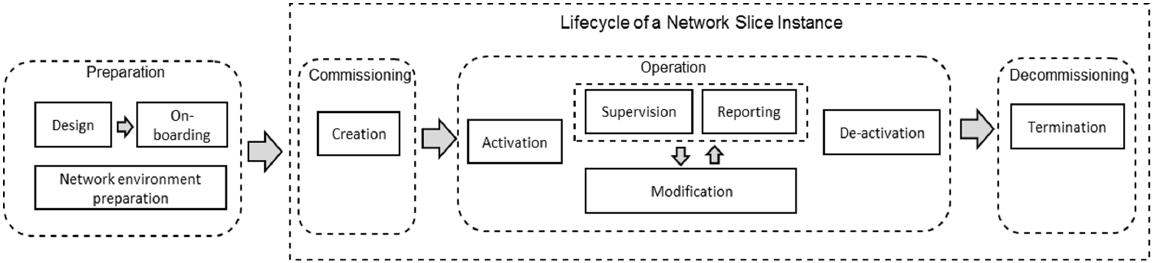
\includegraphics[width=1\linewidth]{figs/NSI_lifecycle.png}
    \caption{\acs{NSI} Lifecycle~\cite{ETSI_MANAGEMENT_ORCHESTRATION_CONCEPTS}}
    \label{fig:slicing:NSI_lifecycle}
\end{figure}

The \acs{NSI} encompasses the full set of Network Function instances and the required resources (e.g. compute, storage and networking resources) of a deployed Network Slice~\cite{ETSI_TS_123_501_V16_9_0} and its corresponding lifecycle is composed by the following phases highlighted in Figure \ref{fig:slicing:NSI_lifecycle}~\cite{ETSI_MANAGEMENT_ORCHESTRATION_PROVISIONING,ETSI_MANAGEMENT_ORCHESTRATION_CONCEPTS}:

\begin{itemize}
    \item \textbf{Preparation:} At this stage, the \acs{NSI} does not yet exist. The \acs{NEST} is created, verified, and onboarded during this phase. It also includes, apart from network slice design, the on-boarding and evaluation of the network functions and all necessary preparations (e.g. network preparations) required before the creation of a \acs{NSI};

    \item \textbf{Commissioning:} The \acs{NSI} is created, which involves allocating and configuring all required resources to satisfy the network slice requirements;
    
    \item \textbf{Operation:} This phase includes the activation, supervision and reporting (related to performance, such as \acs{KPI} monitoring), resource capacity planning, modification and deactivation. The first activates the \acs{NSI}, making it ready to provide communication services, whereas the latter does the opposite. Resource capacity planning involves any actions that calculate resource usage based on \acs{NSI} provisioning and performance monitoring, deriving modification polices as a result of the calculation. \acs{NSI} Modification may be triggered by receiving new network slice requirements or as the result of supervision/reporting and it includes the creation or modification of the \acs{NSI} constituents. Capacity or topology changes correspond to examples of a \acs{NSI} modification;
    
    \item \textbf{Decommissioning:} Encompasses the decomissioning of the required non-shared constituents and the removal of the \acs{NSI} configuration from the shared constituents, after which the \acs{NSI} is terminated and ceases to exist.

\end{itemize}


\subsection{Network Slice Management Functions}

For the purpose of \acs{NSI} management, the concept of a \acf{NSS} is introduced. As outlined in Figure \ref{fig:slicing:class:diagram}, a \acs{NSS} represents a group of network functions (physical and/or virtualized) and their corresponding resources that form part or all of the constituents of a network slice. A \acs{NSS} may be shared between multiple other network slices or subnets and contain instances of \acf{CN} and/or \acf{AN} network functions. Additionally, it may also specify the \acf{TN} requirements necessary to support connectivity between the \acs{CN} and the \acs{AN} network functions within the network slice subnet, covering \acs{TN} topology requirements and individual \acs{TN} links' \acs{QoS} attributes requirements~\cite{ETSI_MANAGEMENT_ORCHESTRATION_CONCEPTS}.

The instantiation of a \acs{NSS} results in a \acf{NSSI}. Similarly, an \acs{NSI} may be composed of one or more \acsp{NSSI} that abide by the same constraints defined for the \acs{NSS} throughout this paragraph. For instance, instantiating an \acs{NSI} with \acs{RAN} and \acs{CN} components may entail defining each domain's component as a separate \acs{NSSI}, potentially shared across multiple \acsp{NSI}~\cite{3GPP-28.801}. Both these constructs must therefore be managed and coordinated correctly to ensure the correct operation of a network slice. 

\begin{figure}[H]
    \centering
    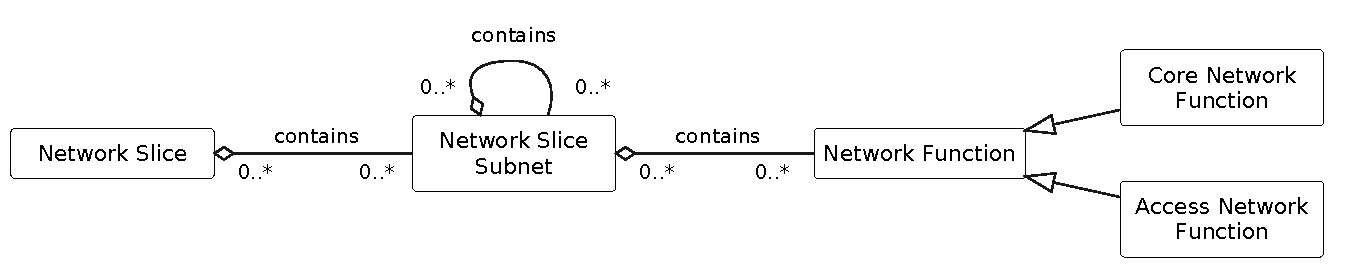
\includegraphics[width=1\linewidth]{figs/plantuml/network-slice-class-diagram.pdf}
    \caption{Network Slice Information Model~\cite{3GPP-28.801}}
    \label{fig:slicing:class:diagram}
\end{figure}

This section identifies three management functions involved in the management and orchestration of network slicing and, consequently, in the support of communication services: the \acf{CSMF}, the \acf{NSMF} and the \acf{NSSMF}. These management functions are organized in a hierarchical structure, where each function delegates part of the related procedures to the next function immediately after it, as showcased in Figure \ref{fig:slicing:management_functions}.

\begin{figure}[H]
    \centering
    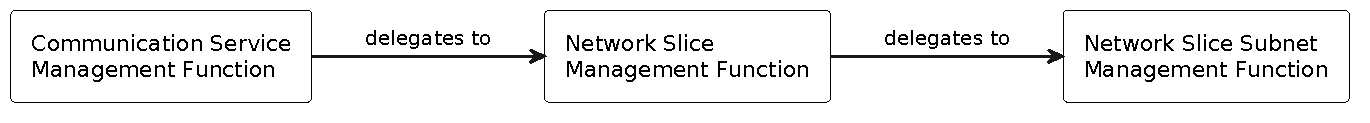
\includegraphics[width=1\linewidth]{figs/plantuml/network-slice-mgmnt-func.pdf}
    \caption{Network Slicing Management Functions~\cite{3GPP-28.801}}
    \label{fig:slicing:management_functions}
\end{figure}

The \acs{CSMF} is responsible for managing the communication services offered by an operator, receiving the requirements requested by end-customers and translating them into concrete network slice requirements, such as network type, network capacity and \acs{QoS} requirements~\cite{3GPP-28.801}. This functionality is closely aligned with that of an \acs{OSS}/\acs{BSS}, which will be further discussed in Section \ref{sota:bss-oss-mano}. These requirements are then forwarded to the \acs{NSMF}, which handles the management of \acsp{NSI} based on the provided requirements. Lastly, the \acs{NSMF} converts the network slice requirements to network slice subnet requirements, which are subsequently delegated to the \acs{NSSMF} for managing and orchestrating \acsp{NSSI}~\cite{3GPP-28.801}.

The management of network slices using these management services must span across the various parts of the network, including both \acs{3GPP} managed network components, such as the \acs{CN} and \acs{AN}, as well as non-\acs{3GPP} components. With this goal, the \acs{3GPP} management system derives each domain's requirements from the customer's service requirements (for a given communication service) and forwards them to the corresponding domain management systems, coordinating the exchange of data between them. For components outside the \acs{3GPP} domain, such as the \acs{TN}, this implies coordinating with the corresponding external management systems to communicate the network slice requirements~\cite{ETSI_MANAGEMENT_ORCHESTRATION_CONCEPTS}.

This is especially relevant, not only in the context of the \acs{TN}, but also considering the inherent virtualization nature of network slicing. When an operator wants to create a network slice, i.e. a \acs{NSI} that includes virtualized network functions, the \acs{NSSMF} should, per request from the \acs{NSMF}, create the needed \acsp{NSSI}, according to the network slice requirements. This involves coordinating with an external management system, namely the \acs{NFV-MANO}, to instantiate and configure all \acsp{VNF} and \acsp{NS}, scaling them as needed for the operations of the \acs{NSI}, while accounting for the fact that these resources may be shared by multiple \acsp{NSSI}. Only after coordinating with the \acs{NFV-MANO}, and performing the necessary application level configurations to the \acsp{NF} allocated to the \acs{NSSI}, the \acs{NSMF} can proceed with the activation of the \acs{NSI}~\cite{3GPP-28.801}.

\subsection{Network Slice Managers}

A Slice Manager is a software system that allows the orchestration and lifecycle management of network slices. The following section presents an overview of two slice managers: the Katana Slice Manager and \acs{ITAv}'s Slice Manager.

\subsubsection{Katana Slice Manager}

Katana is a slice manager solution developed as a part of the 5GENESIS project~\cite{KatanaSliceManagerGenesis}. Through its \acf{NBI}, it receives the \acs{NEST} for creating the network slices, providing an \acs{API} for managing and monitoring them. The \acs{NEST} descriptor, specified in \acs{YAML} or \acs{JSON}, specifies the network slice characteristics and parameters, including \acs{NFV} components, \acs{QoS} monitoring level and Life-Cycle stages. Based on the onboarded \acs{NEST}, the slice manager maps the available data plane resources to the described slice requirements in order to create the requested slice. Additionally, the slice manager communicates with the components from the Management Layer through its \acs{SBI}, including the \acf{VIM}, \acf{NFVO}, \acf{EMS} and \acf{WIM}.

To accommodate multi domain testbed environments, it was developed as a standalone solution that interacts with other components of the \acf{MANO} layer via the defined interfaces (e.g. through SOL005 interface for \acf{OSM} \acf{NFVO}), as to allow the management of the network slice's lifecycle without extended \acs{MANO} functionality~\cite{KatanaSliceManagerGenesis}

\begin{figure}[H]
    \centering
    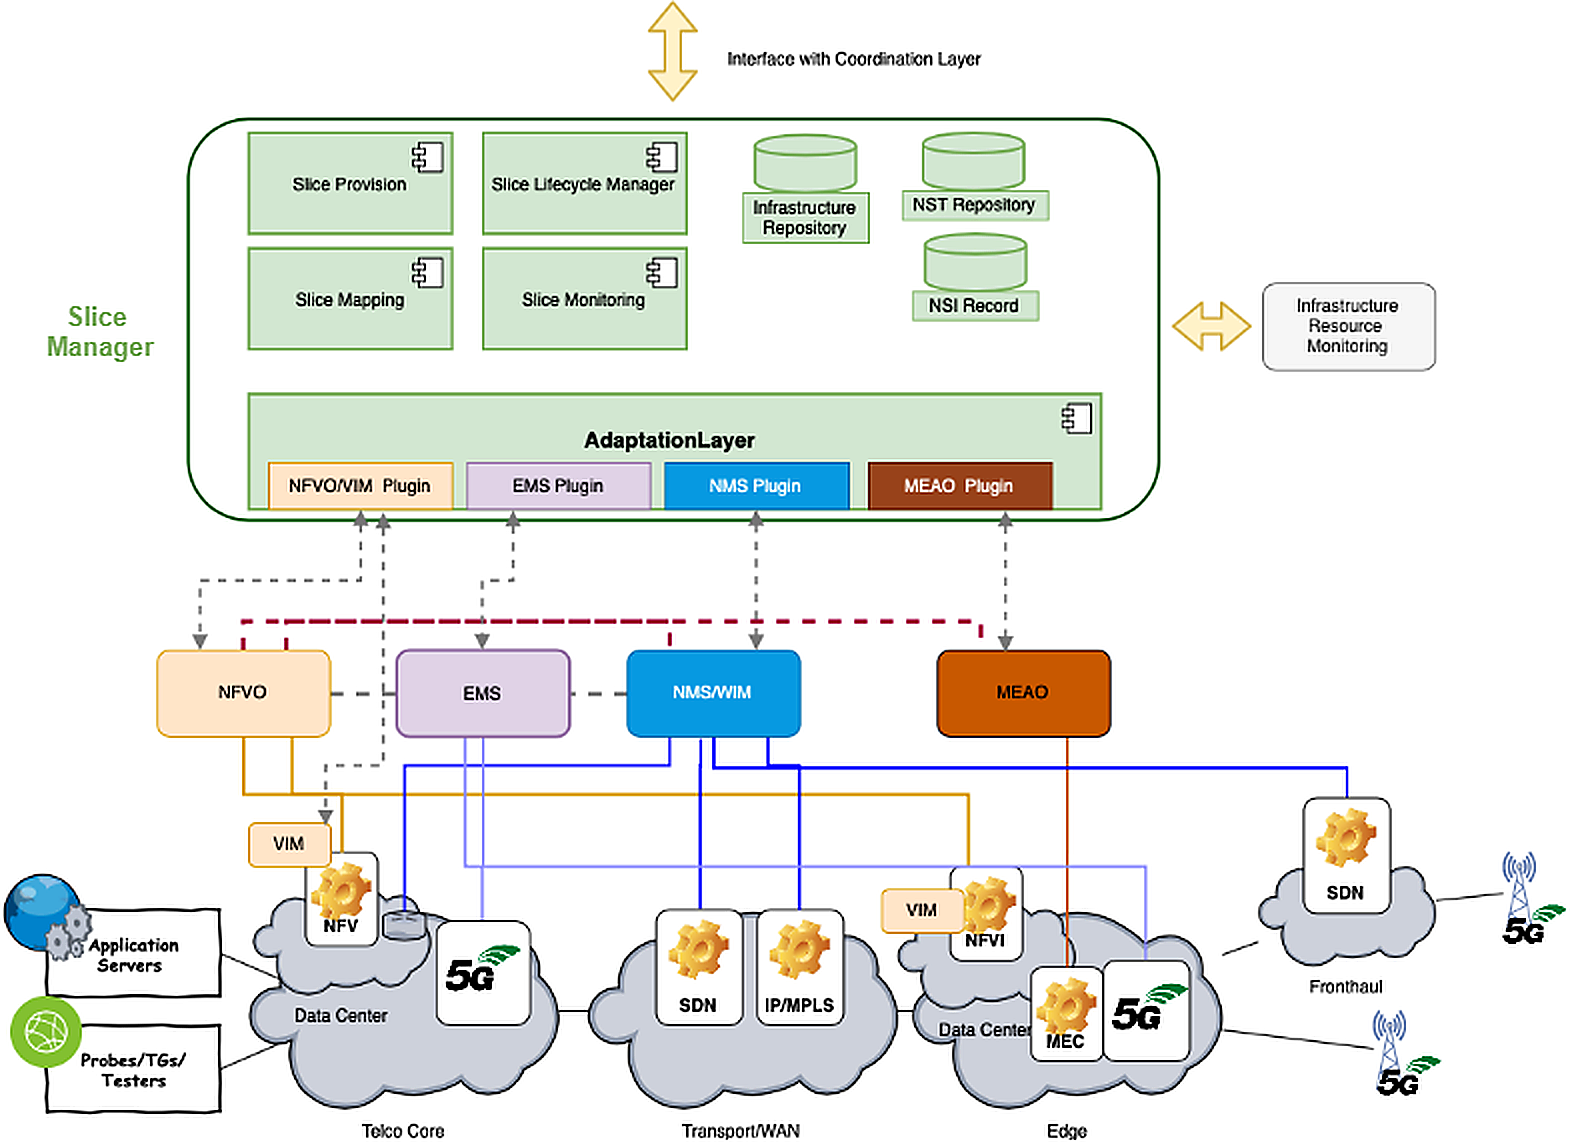
\includegraphics[width=0.95\linewidth]{figs/katana-architecture-upscaled.png}
    \caption{Katana Slice Manager Architecture~\cite{KatanaSliceManagerWiki}}
    \label{fig:katana:architecture}
\end{figure}


The Katana Slice Manager follows a highly modular architecture, implemented as a mesh of independent microservices, each running in a dedicated Docker container. Figure \ref{fig:katana:architecture} illustrates the architecture of the slice manager, highlighting its constituent modules and their interconnections, as described bellow~\cite{KatanaSliceManagerWiki}.

\customparagraph{North Bound Interface API}

The \acf{NBI} provides a set of \acs{REST} \acsp{API}, to be consumed by a component of the coordination layer, such as the Experiment Lifecycle Manager. It includes two submodules that consume these \acs{REST} \acsp{API}, allowing a user or admininstrator to interact with it: (i) a \acf{CLI} for Bash commands interaction via the terminal and a (ii) web \acf{GUI} that interacts with the Slicing Lifecycle Manager and repositories to create new slices. 

\customparagraph{Slicing Lifecycle Manager}

This module serves as the central component of the slice manager, responsible for managing the lifecycle of network slices through \acs{CRUD} operations. It handles requests from the \acs{NBI} \acsp{API} and executes the required actions to activate, modify or deactivate a network slice. Additionally, it receives status updates from the Slice Monitoring module regarding a given slice, coordinating with other components to trigger the appropriate processes in response to these changes. Lastly, it is also tasked with optimally selecting the infrastructure resources to be used for a new slice, according to the available resources and the slice requirements, during the slice creation phase.

\customparagraph{Slice Mapping}

The Slice Mapping component manages the slice mapping process, following the request for a new slice. It maps the \acs{GST} requests with a specific \acs{NEST} that is supported by the infrastructure.

\customparagraph{Slice Provisioning}

Receives requests from the Slicing Lifecycle Manager service to setup, configure or delete \acs{WAN} paths, isolated \acs{NFVI} tenant spaces and the related network services. It also manages the configuration of radio component parameters and the registration of the newly created slice into the Monitoring system. All of the aforementioned functionalities are achieved by utilizing plugins of the Adaptation Layer.

\customparagraph{Slice Monitoring}

This module is responsbile for monitoring the health and the status of every deployed slice. Similarly to the previous service, it relies on Adaptation Layer plugins to send status check messages to the \acs{MANO} components and report status changes to the Slicing Lifecycle Manager.

\customparagraph{Adaptation Layer}

The Adaptation Layer provides an abstraction layer over the underlying technology, allowing the slice manager to operate over any \acs{MANO} layer component without any modifications to its core functionality, given the correct plugin is installed. This module includes plugins for each of the slice manager's \acs{MANO} layer components, which are responsible for receiving and translating requests from the Slicing Lifecycle Manager into the corresponding component \acs{API}, and, consequently, processing the responses.


This architecture provides the baseline for the provisioning and lifecycle management of network slices. However, the Katana open source project has been inactive, with no updates since December 2022, rendering it unusable for this dissertation. It does not support more recent \acs{OSM} versions, with the latest compatible release being \acs{OSM} 8.


\subsubsection{ITAv Slice Manager}

\acf{ITAv} has its own proprietary implementation to automate the deployment and management of network slices in \acs{5G} networks~\cite{ITAvSliceManager}. The \acs{ITAv} Slice Manager is currently deployed on the 5GAIner testbed~\cite{5GAIner}, a commercial-grade \acs{5G SA} infrastructure also available at \acs{ITAv}. The solution enables the programmatic reconfiguration of the \acs{5G} network, provisioning slices tailored to meet the requirements of the three primary \acs{5G} services: \acs{eMBB}, \acs{URLLC} and \acs{mMTC}/\acs{MIoT}. The slices configured by the network slice manager preserve the network \acf{TRL}, being the produced
slices representative of a commercial-graded solution. Moreover, the slice manager also offers dynamic slicing capabilities, supporting the adaptation of the slice performance in real time without communication disruption.

The \acs{ITAv} Slice Manager is designed with a strong focus on adherence to established standards to ensure interoperability and seamless interaction with other software systems, as defined by \acs{3GPP}. In particular, it complies with the following specifications:

\begin{itemize}
    \item 3GPP TS 28.531 version 18.3.0~\cite{ITAv_3gpp_28531_v18_3_0}: outlines the essential Network Functions for a standardized network slice manager;
    
    \item 3GPP TR 28.824 version 18.1.0~\cite{ITAv_3gpp_28824_v18_0_1}: identifies the \acf{TMF} standards required for the Slice Manager, with adherence to TMF622\_ProductOrder~\cite{TMF622UserGuideV5} and TMF641\_ServiceOrder~\cite{TMF641UserGuideV411}, as defined in December 2023;

    \item 3GPP TS 28.541 version 18.4.1~\cite{ITAv_3gpp_28541_v18_4_1}: delineates the profiles associated with network slices (e.g. ServiceProfile, TOPSliceSubnetProfile);

    \item 3GPP TS 28.530 version 17.4.0~\cite{ITAv_3gpp_28530_v17_4_0}: presents the Network Slice Management Lifecycle.
\end{itemize}

According to the original work~\cite{ITAvSliceManager}, the \acs{ITAv} Slice Manager supports an extensive list of Slice Manager requirements identified throughout the literature: \ac{E2E} Slice Support, Slice Lifecycle Management, Network Configuration, Policy and \acs{QoS} Management for \acs{SLA} Enforcement, Dynamic Slicing, Custom Slices, Network Slice Monitoring, Location-based Slicing, Performance Assurance, Multiple Slice Management, Network Resource Monitoring, Slice Feasibility Evaluation, and Generic Network Support. Furthermore, the slice manager solution can be integrated with \acs{OSM} and \acf{OSL}, allowing adherence to an even more complete set of requirements with orchestration and \acf{OSS} capabilities~\cite{ITAvSliceManager}. The \acs{ITAv} Slice Manager represents a significantly more mature solution than the available alternatives.



\section{NFV} \label{sota:nfv}

As outlined in Section \ref{sota:5gecosystem}, the implementation of network slicing is supported by virtualization technologies, such as \acs{SDN} and \acs{NFV}, which have fundamentally transformed how networks are managed and deployed. With the growing adoption of \acs{SDN} and \acs{NFV} technologies, network functions are no longer tied to dedicated hardware instead being instantiated dynamically as software components in cloud environments. This allows operators, partners and even subscribers to create instances of their services and networks on demand~\cite{EricsonOSS}. 

This section examines the concept of \acs{NFV} and its realization through the \acf{NFV-MANO} framework. It provides an analysis of the \acs{NFV-MANO} architecture and its constituent functional blocks, detailing their respective roles and interactions in enabling the deployment and orchestration of virtualized network services.


\subsection{NFV-MANO Architectural Framework}

As previously stated, \acs{NFV} refers to the principle of separating network functions from the underlying running hardware using virtualization techniques. This approach results in \acfp{VNF}, software solutions that realize all or part of a \acf{NF} and can be deployed in the \acf{NFVI}~\cite{ETSI_GR_NFV_TERMINOLOGY_003_V1_9_1}. A \acf{NS} is then defined as the composition of one or more \acsp{NF} (\acsp{VNF} or \acsp{PNF}) and/or other \acsp{NS} to deliver \acs{E2E} services, along with the \acfp{VL} connecting them~\cite{ETSI_GS_NFV_006_V5_2_1}. The behavior of the constituting \acs{NS} is derived from the combination of its individual \acs{NF} behaviours and of the network infrastructure composition mechanism. The deployment and operational requirements of a \acs{NS} are described in a \acf{NSD}, describing the service topology, network service characteristics (e.g. \acsp{SLA}) and other depedendencies necessary for its onboarding and lifecycle management~\citep{ETSI_GS_NFV_MAN_001_V1_1_1,ETSI_GR_NFV_TERMINOLOGY_003_V1_9_1}.

The \acs{NFV-MANO} architectural framework is responsible for managing the \acs{NFVI} and orchestrating the allocation of resources needed by \acsp{NS} and \acsp{VNF}, as well as performing lifecycle management operations for \acsp{NS} and \acsp{VNF}~\citep{ETSI_GS_NFV_MAN_001_V1_1_1,ETSI_GS_NFV_006_V5_2_1}. As described in Figure \ref{fig:nfv-mano-architecture}, it is composed by the following four functional blocks~\cite{ETSI_GS_NFV_006_V5_2_1}:

\begin{itemize}
    \item \textbf{\acf{NFVO}:} responsible for the orchestration of \acs{NFVI} across multiple \acsp{VIM} and the lifecycle management of \acsp{NS} and their constituent resources. Through the \texttt{Os-Ma-nfvo} reference point, it provides an entrypoint for \acs{OSS}/\acs{BSS} to interact with the \acs{NFVO} to invoke management operations of \acsp{NSD} and to subscribe to notifications related to \acs{NSD} management changes, as specified in \acs{NFV}-SOL 005~\cite{ETSI_GS_NFV_SOL_005_V5_3_1};
    \item \textbf{\acf{VNFM}:} handles a set of management functions focused on the creation and lifecycle management of \acsp{VNF}. These include \acs{VNF} lifecycle management, \acs{VNF} configuration management, \acs{VNF} information management, \acs{VNF} performance management and \acs{VNF} fault management. It interacts with the \acs{NFVO} through the \texttt{Or-Vnfm} reference point, allowing it to invoke \acs{VNF} lifecycle management operations of \acs{VNF} instances and to subcribe to notifications regarding \acs{VNF} lifecycle changes provided by the \acs{VNFM}, as specified in \acs{NFV}-SOL 003~\cite{ETSI_GS_NFV_SOL_003_V5_3_1};
    \item \textbf{\acf{VIM}:} controls and manages the \acs{NFVI} virtual resources used by \acsp{VNF} and \acsp{VL}, regarding compute, storage and network resources. To achieve this, it exposes a \acs{NBI} for the management of \acs{NFVI} virtualized compute, storage and network resources;
    \item \textbf{\acf{WIMNFV}:} allows management of network connectivity between connectivity service endpoints, located in different sites. The \acs{WIM} performs path computation based on quality assurance factors such as jitter, round-trip time, and bandwidth requirements, establishing connectivity over the physical network~\cite{ETSI_GS_NFV_MAN_001_V1_1_1}. Within the architectural framework, the \acs{WIM} may be integrated as a part of \acs{NFV-MANO}, as depicted in Figure \ref{fig:nfv-mano-architecture}, or exist as an external component, for example, under the control of the \acs{OSS}.
\end{itemize}

\begin{figure}[htpb]
    \centering
    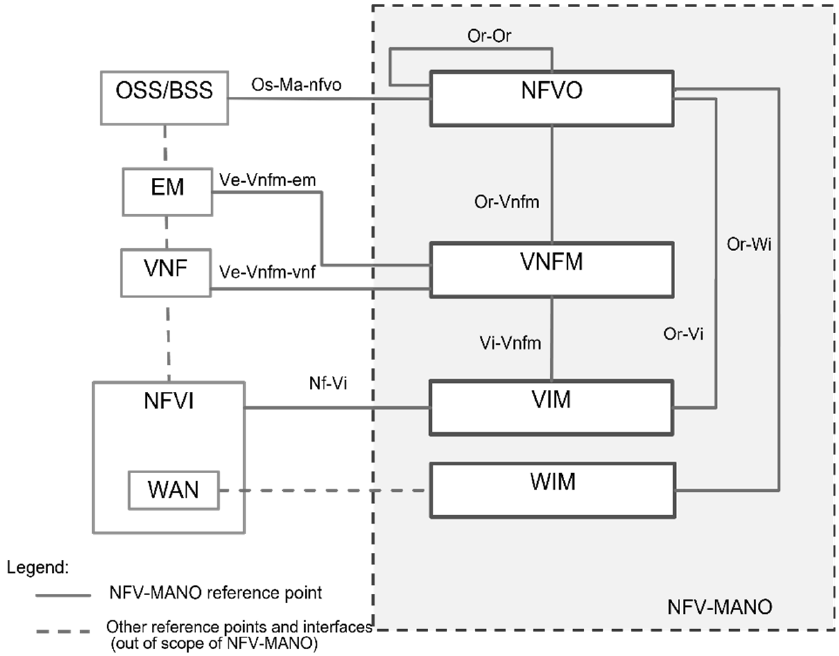
\includegraphics[width=1\linewidth]{figs/NFV-MANO-architecture.png}
    \caption{NFV-MANO architectural framework~\cite{ETSI_GS_NFV_006_V5_2_1}}
    \label{fig:nfv-mano-architecture}
\end{figure}

\clearpage

Over the years, multiple open source \acs{MANO} solutions, compliant with \acs{ETSI} \acs{NFV-MANO} have been implemented, such as the \acs{ETSI}  \acs{OSM}~\footnote{\url{https://osm.etsi.org/}}. By leveraging interfaces as the \acs{NFV}-SOL 005, it provides \acs{REST} \acsp{API} necessary for the integration with \acs{OSS}/\acs{BSS} systems, such as \acf{OSL}. This allows a more coordinated and integrated approach, yielding a series of benefits. The integration between \acs{NFV-MANO} and \acs{OSS}/\acs{BSS} systems and their benefits is further explored in Section~\ref{sec:oss:bss:nfv-mano}.





\section{5G SBA} \label{sota:sba}


The \ac{3GPP} specification for the \ac{5G} system architecture is defined to support data connectivity and services across a wide range of heterogeneous applications with diverse requirements. The \acs{5G} System adopts a \ac{SBA} with a modular and stateless \ac{NF} design, which segregates \ac{UP} and \ac{CP} functions for independent scalability and evolution. This architecture facilitates flexible deployment, where authorized \acp{NF} can access each other's services through reusable service procedures. The \ac{3GPP} TS \text{23.501} specification also identifies, among other key aspects, support for a unified authentication framework, discussed in Section \ref{sota:initiatives:CAPIF}, as well as analytics and capability exposure functionality, for third-party access, the latter of which will be analyzed in this section~\cite{ETSI_TS_123_501_V16_9_0}.

Figure \ref{fig:5g-sba} depicts the service-based representation of version \text{18.11.0} Release 18 of the Non-Roaming \acs{5G} System Architecture~\cite{ETSI_TS_123_501_V16_9_0}. It includes service-based interfaces (e.g. Nnef) for network function interaction within the \acl{CP}, as well as point-to-point reference points (e.g. N1) for interactions with \acl{UP} functions and entities (i.e \ac{UE}, (R)AN, \ac{UPF} and \ac{DN}).

\begin{figure}[htbp]
    \centering
    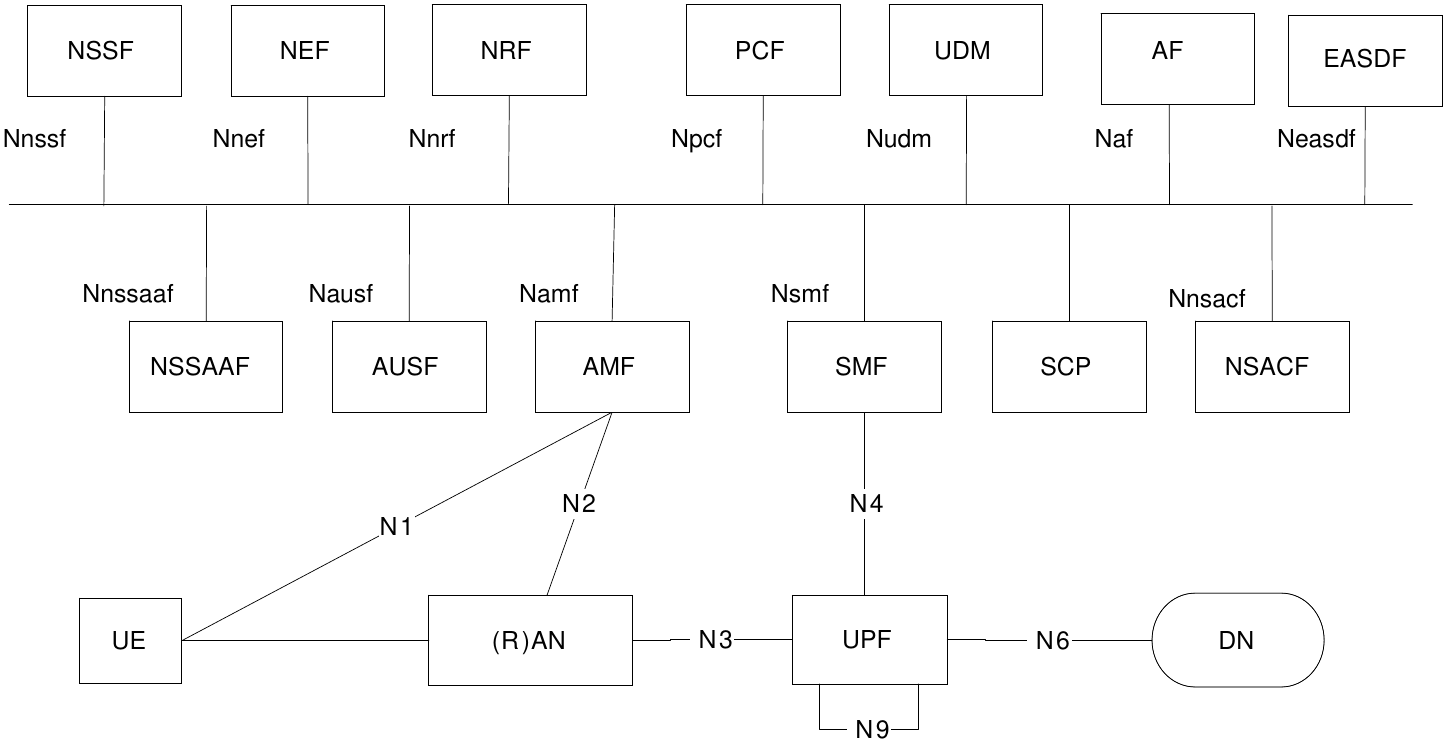
\includegraphics[width=1\linewidth]{figs/5G-SBA.png}
    \caption{Non-Roaming \acs{5G} System Architecture~\cite{ETSI_TS_123_501_V16_9_0}}
    \label{fig:5g-sba}
\end{figure}

The \acs{5G} System architecture consists of the following network functions:

\begin{itemize}
    \item{\textbf{(Radio) Access Network ((R)AN):}} access network that provides \ac{UE} connectivity to the \ac{5GC} Network, including \acf{NG-RAN} and/or non-3GPP access technologies;

    \item{\textbf{\acf{DN}:}} external data network that provides access to operator services, third-party services or the Internet;

    \item{\textbf{\acf{AUSF}:}} supports authentication for both, \acs{3GPP} access and non-3GPP access (untrusted access via \acs{N3IWF}, trusted access via \acs{TNGF} and wireline access via \acs{W-AGF}). Its most significant functionalities include providing, to requester \acs{NF}, \acs{UE} authentication and protection mechanisms for \ac{SoR} information and \acs{UE} parameter updates;

    \item{\textbf{\acf{SMF}:}} handles \ac{PDU} session management (establishment, modification and release) and \ac{UE} \ac{IP} address allocation, including selecting and controlling the \ac{UPF} to steer traffic to the proper destination; 
    
    \item{\textbf{\acf{AMF}:}} responsible for registration, connection, reachability and mobility (e.g. handover) management between the \ac{UE} and the network. It also acts as an intermediary transport forwarding \ac{SM} messages between \acp{UE} and the \ac{SMF};

    \item{\textbf{\acf{PCF}:}} governs network behaviour based on a unified policy framework by providing policy rules to control plane functions that enforce them throughout the network. These policies cover, for example, charging, \acs{QoS} and network slicing scenarios (e.g. limits data rate per network slice). To facilitate these decisions, the \acs{PCF} accesses relevant subscription information from the \acs{UDR}, both located in the same \acs{PLMN}\hide{\later{explain this somewhere and PLMN too}};

    \item{\textbf{\acf{NSSAAF}:}} responsible for authentication and authorization mechanisms specific to a slice;

    \item{\textbf{\acf{NEF}:}} provides secure exposure of \acs{NF} capabilities and events to third parties, \acsp{AF} and edge computing environments, allowing them to interact with the network through standardized interfaces. It manages the secure provisioning of information from external applications to the internal network (e.g. authentication, authorization and assist in throttling \acsp{AF}), handling the necessary translation of data between the two domains (e.g. masking of network and user sensitive information to external \acsp{AF}'s according to the network policy). By interacting with other \acsp{NF}, namely the \acs{NWDAF}, \acs{NEF} supports the exposure of \acs{NWDAF} analytics to external parties, mediating the collection of data by the \acs{NWDAF} and forwarding requests and notifications between it and the \acs{AF};

    \item{\textbf{\acf{UDM}:}} handles subscription management and access authorization based on subscription data (e.g. roaming restrictions). It is also responsible for registering and storing the \acp{NF} actively serving \acp{UE} (e.g. \ac{SMF} registration with the \ac{UDM} upon establishment of a \ac{PDU} session), which is specially relevant for service continuity (e.g. tracking \ac{SMF}-\ac{DNN} assignments of ongoing sessions);

    \item{\textbf{\acf{UPF}:}} provides an interconnection point through which external \ac{PDU} sessions connect to the \ac{DN}, handling packet routing and forwarding, such as uplink traffic between \acp{UE} and an instance of a \ac{DN}. It's also responsible for handling \ac{QoS} and policy rule enforcement within the user plane;

    \item{\textbf{\acf{AF}:}} interacts with the \ac{CN} to provide services, influencing aspects such as traffic routing, \ac{QoS} (e.g. request \acs{AF} session with required \ac{QoS}), policies and charging. Based on the deployment, \acsp{AF} considered to be trusted by the operator, as represented in Figure \ref{fig:5g-sba}, can interact directly with the rest of \acsp{NF}, whereas untrusted \acsp{AF} are required to access network function capabilities through the \acs{NEF};\hide{\later{maybe give examples}}

    \item{\textbf{\acf{SCP}:}} supports indirect communication between \acp{NF}' services, forwarding and routing messages either to the destination \acs{NF} service or to a subsequent-hop \ac{SCP}. It also ensures communication security, as well as load balancing, monitoring, and overload control;

    \item{\textbf{\acf{NRF}:}} supports service decovery, allowing \acp{NF} to discover other \acp{NF} and their services, as well as \acs{SCP} discovery by other \acsp{SCP}. It achieves this by maintaining the current health status and profiles of available \ac{SCP} instances and \ac{NF} instances and their supported services. Additionally, it notifies subscribed consumers whenever a \ac{NF} or \ac{SCP} instance is registered, updated, or deregistered;

    \item{\textbf{\acf{NSSF}:}} responsible for selecting the Network Slice instances serving a specific \ac{UE}, tailored for specific service requirements. This includes determining the \ac{NSSAI} and, if needed, the mapping to the subscribed \acp{S-NSSAI};

    \item{\textbf{\acf{NWDAF}:}} collects and analyses data from the \ac{5G} network, leveraging information obtained from \acp{NF} (directly or via \ac{NEF}) and \ac{OAM} systems, with the goal of optimizing the \acs{5G} network's operation and service quality. \ac{NWDAF} consumers, i.e. \ac{5GC} \acp{NF} and \ac{OAM}, use the data analytics provided by the \ac{NWDAF} to assess, inter alia, slice's load level information, observed service experience, \ac{NF} load, network performance (e.g. \ac{gNB} status and resource usage) and \ac{QoS} Sustainability (e.g. \ac{QoS} change statistics). Analytics information are either statistical information on past events or predictive information (e.g. \ac{NF} load or network performance predictions, likelihood of a \ac{QoS} change) and can be obtained through the use of \ac{ML} models~\cite{ETSI_TS_123_288_V18_11_0}.

    

    % Lacks EASDF, NSACCF

\end{itemize}

\hide{

mention virtualization and softwarization

NFV and SDN

transition to a software-driven architec-
ture, emphasizing virtualization and cloud technologies, and
adopted a Service-Based Architecture (SBA) for scalable and
modular Network Functions (NFs)

scalable evolve indepedntly
}

\subsection{Network Analytics Capabilities}

The introduction of \ac{NWDAF} and its data collection, analytics and predictive capabilities, unlocks the possibility for data-driven network solutions that automate network management and optimize resource allocation~\cite{AdvancingPredictiveSecurity}. Capitalizing on this potential, several studies in the literature have explored various use cases for the \ac{NWDAF}, including solutions in network security and threat mitigation, as well as resource and operational efficiency. In the context of network security and threat mitigation, \ac{NWDAF} can, from collected data from functions such as the \ac{SMF}, \ac{AMF}, \ac{AF} and \ac{UPF}, identify abnormal user behavior and specific types of \ac{DDoS} attacks detecting UDP fragmentation, SYN, ICMP, DNS, and GTP flood attacks~\citep{AdvancingPredictiveSecurity,UserTerminalsAsAttackers}. This \ac{NWDAF} functionality can be extended to any anomaly detection scenarios in sectors such as logistics, maritime, and smart cities, where it can monitor communication patterns from vehicles, vessels or \ac{IoT} sensors to identify irregularities indicative of hijacking, system malfunctions or cyber-attacks~\cite{UserTerminalsAsAttackers}. Regarding resource and operational efficiency, the \ac{NWDAF} is capable of analysing \ac{RAN} data, \ac{UPF} traffic and \acs{CPU} usage to predict network load and resource utilization, and proactively allocate additional resources when necessary, preventing performance degradation with faster response times than a simple threshold-based strategy~\cite{ExplorationNWDAFDevelopmentArchitecture6G}.


Additionally, the operation of the \ac{NWDAF} in conjunction with other \aclp{NF}, namely the \acs{NSSF}, supports automatic slice selection mechanisms with data collected and analysed by the \ac{NWDAF}. By evaluating \acs{QoS} and \acs{QoE} metrics and leveraging machine learning models, the network can dynamically select the most suitable vertical slices, acommodating a variety of \ac{IoT} use cases such as vehicular or real-time health systems~\cite{NetworkSliceSelectorIoT}.

\subsection{Network Exposure Capabilities} \label{sec:network:exposure:mechanisms}

The exposure of network capabilities has introduced a new level of flexibility for users and applications, allowing them to leverage and influence the capabilities of the network rather than being constrained by the functionalities explicitly offered by the mobile network. By granting access to third party external applications, this also opens the possiblility for telecom \acsp{SP} to monetize their network capabilities. With this objective, \acs{3GPP} has specified a series of Capability Exposure frameworks through the use of Northbound \acsp{API} and Application Enabler Layer \acsp{API}~\cite{CapabilityExposure3GPP}.

\subsubsection{\acl{NEF}} \label{sec:sba:nef}

The core network function responsible for \acs{5G}'s network capability exposure is the \acs{NEF}. The \acs{NEF} securely exposes \acsp{NF}' capabilities to external third parties, providing a set of northbound \acsp{API} through which they can interact with the \ac{5GC} to build network-aware applications. Thus, the \acs{NEF} allows service providers to access network capabilities contributing to the concept of an open and programmable network, while abstracting them from the underlying network~\cite{NEFsim}. More specifically, \acs{NEF} offers an exposure layer composed of northbound \acsp{API}, which are then internally connected to the \acs{SBA} southbound \acsp{API} to provide the intended functionalities, such as exposing network data and receiving management commands~\cite{CAPIFmicroserviceVerticals}. This and all other exposure capabilities supported by the \acs{NEF} can be classified into the following categories~\cite{ETSI_TS_123_501_V16_9_0}:
\begin{itemize}
    \item \textbf{Monitoring capability:}  monitoring of specific \acs{UE} events in the \acs{5G} System and making the correponding event information available for external exposure via the \acs{NEF}. Monitoring capability supports exposing \acs{UE}'s mobility management context such as \acs{UE} location, reachability, roaming status and loss of connectivity, as well as \acs{QoS} monitoring results. It includes functionality for identifying the \acs{5G} network function most suitable for configuring the specific monitoring events, detecting the monitoring event and reporting it to the authorised external party;
    
    \item \textbf{Provisioning capability:} allows an external party to provision information that can be used for the \acs{UE} in the \acs{5G} System. Provisioning Capability permits the external party to provision Expected \acs{UE} Behaviour, \acs{5G-VN} group information or service specific information to a \acs{5G} \acs{NF}. It comprises of the authorisation of the provisioning external third party, receiving the provisioned external information via the \acs{NEF} and storing and distributing it to the requiring \acsp{NF};
    
    \item \textbf{Policy/Charging capability:}  handling access and mobility management, \acs{QoS} and charging policies for the \acs{UE} based on a request from an external party. More specifically, it has mechanisms for handling a specific \acs{QoS}/priority setting for an \acs{UE} session and configuring the applicable charging party or charging rate;
    
    \item \textbf{Analytics reporting capability:} enables an external party to fetch, subscribe or unsubscribe to analytics information generated by the \acs{5G} System. Analytics reporting capability incorporates functionality for discovering the type of analytics available to an external party and requesting analytics information generated by the \acs{NWDAF} for consumption;

    \item \textbf{Member \acs{UE} selection capability:} allows an external party to acquire one or more list(s) of candidate \acs{UE}(s), selected from the list of target member \acs{UE}(s) provided by the \acs{AF}, along with additional information derived from assistance information generated by the \acs{5G} System based on predefined filtering criteria.

\end{itemize}


\subsubsection{Application Enabler Layer}

Unlike the previous generations, \acs{5G} focuses on enabling vertical applications integrated with the underlying \acs{5G} network, potentially providing \acsp{MNO} with new revenue streams and shifting away from traditional \acf{B2C} models, with an end-user, toward \acf{B2B} opportunities, with industry verticals~\cite{SEAL5GVerticals}. To capitalize on the monetization of their network capabilities while tailoring to the needs of the various vertical sectors, \acs{3GPP} has defined capability exposure frameworks based on Application Enabler Layer \acsp{API}. 

Application Enabler Layer \acsp{API} are abstraction layers for specific vertical applications (e.g. Edge, \acs{UAS}, \acs{V2X}) or common to multiple vertical applications, which allow the exposure of common core and application enabler services to external applications. This abstraction is provided in paralell or on top of abstraction functionalities already provided by Network Northbound \acsp{API} via the \acs{NEF} or any other network \acsp{API} (e.g. network management \acsp{API}) to fullfill requests from vertical applications~\cite{CapabilityExposure3GPP}.

The Application Enabler Layer \acsp{API} designed to be common for multiple vertical applications are securely provided to verticals through the \acf{SEAL}~\cite{ETSI_TS_123_434_V18_12_0_SEAL}. The \acs{SEAL} defines a standardized functional architecture considering the common capabilities required to support multiple vertical applications over \acs{3GPP} networks. These capabilities are accessible for use through the following \acs{SEAL} services: Location management, Group management, Configuration management, Identity managemen, Key management, Network resource management, Data delivery, Notification management, Network slice capability enablement and Application data analytics enablement~\cite{ETSI_TS_123_434_V18_12_0_SEAL}. Many of these capabilities correspond to auxiliary services that address cross-cutting concerns, common across verticals. Developing them independently for each vertical would be redundant and require substantial time and effort. Instead, vertical application developers can focus exclusively on the core features and functionalities of the vertical application, while utilizing \acs{SEAL} for the auxiliary services, thus saving significant time and cost to market~\cite{SEAL5GVerticals}.

In addition to \acs{SEAL}'s common reusable services across multiple vertical sectors, a dedicated service framework is required to address the specific requirements of edge-based services and edge computing. Edge Computing is a network architecture concept that deploys cloud computing capabilities and service environments close to the \acsp{UE}, with the goal of achieving several benefits, such as lower latency, higher bandwidth, reduced backhaul traffic and possibly new innovative services not feasible or supported in regular cloud environments. With this goal, \acs{3GPP} specifies an application architecture for enabling Edge Applications on the \acf{EDN}. More specifically, it introduces the \acf{EEL} to facilitate communication between the \acfp{AC} running on an \acs{UE} and the \acf{EAS} deployed on the \acs{EDN}. Regarding network exposure capabilities, the \acs{EEL} exposes northbound \acsp{API} towards the \acsp{EEC} (running on an \acs{UE}), \acsp{EAS} (possibly third-party \acsp{EAS} outside the \acsp{ECSP} trust domain) and other internal functional entities. These services encompass native \acs{EEL} services, such as service provisioning, \acs{EAS} discovery and support for service continuity, as well as enhanced re-exposed services of the \acs{3GPP} \acs{CN}, such as \acs{UE} Location and \acs{QoS} sessions. While distinct in their application, both categories utilize the exposed network capabilities via \acs{NEF} northbound \acsp{API}, optionally via \acs{CAPIF}. Native services consume these network capabilities to support internal logic, such as retrieving a \acs{UE}'s location to filter discovery results, whereas re-exposed services are built directly on the \acs{NEF} capabilities to provide enhanced access to network functions~\cite{ETSI_TS_123_558_V18_11_0_EDGE}.

The previously mentioned enabler layers focus on generic application support for multiple vertical applications and edge applications, respectively. To address the diverse requirements of heterogeneous vertical use cases, additional vertical-specific enabler layers were defined. The \acf{VAE} layer ensures efficient use and deployment of \acs{V2X} applications on \acs{3GPP} networks, supporting use cases such as platooning, remote and tele-operated driving, \acs{HD} maps and Vehicle-to-Pedestrian communication with \acf{VRUP}. It serves as an abstraction layer that encapsulates the underlying mechanisms from the \acs{V2X} application specific layer and exposes them via northbound \acsp{API}, providing interfaces for operations such as group management and message distribution. To support these functionalities, the \acs{VAE} utilizes the \acs{NEF} for interacting with the \acs{5G} System, allowing it to receive \acs{QoS} monitoring information and network data analytics (e.g. congestion status reported by the \acs{NWDAF} to \acs{NEF}). It also relies on \acs{SEAL} for support services in location management, group management, configuration management, identity management, key management and network resource management, thus emphasizing the importance of these components in the \acs{V2X} vertical-specific scenario~\cite{ETSI_TS_123_286_V19_0_0_V2X}.

Similar enabler layers exist for other vertical sectors in \acf{UAS}~\cite{ETSI_TS_123_255_V18_2_0_UAS}, \acs{5G} messaging for \acf{MIoT} communication~\cite{ETSI_TS_123_554_V18_10_0_Messaging} and \acf{FF}~\cite{3GPP_23_745_V17_0_0_FF}. All provide abstraction layers for vertical specific capabilities, exposing northbound \acsp{API} that may require interactions with the \acs{NEF} and \acs{SEAL} components to fulfill these capabilities, optionally via \acs{CAPIF}.



\subsubsection{NEF Implementations} \label{exposure:NEFimplementations}

In regards to \ac{NEF} implementations, there are a variety of implementations across both open source \acs{5G} core solutions and in commercial deployments. This section provides an overview of the current \ac{5G} \ac{NEF} solutions and their supported northbound \acsp{API} and services, followed by a discussion of their level of adoption in the literature. 

Concerning commercial solutions, Nokia's \ac{NEF}~\cite{NokiaNEF2022} is described as a cloud native \ac{PaaS} following a microservices architecture with a \ac{REST} aproach. However, proprietary commercial solutions are constrained by licensing restrictions, making free and open-source alternatives more viable.

As for open source projects, the presence of the \ac{NEF} component varies across different \ac{5G} core implementations. For instance, Open5GS, despite providing a C-based implementation of a \ac{5G SA} Core with a \ac{SBA} architecture supporting a wide variety of network functions, it still lacks a \ac{NEF} implementation~\cite{Open5GSDocs}. Consequently, authors have resorted to extending the Open5GS \acs{CN} by developing and integrating their own \ac{NEF} solutions~\citep{CloudEnabledDeployment5GN, DynamicQoSAdaptationviaExposedServiceAPIs}. The \ac{5G} \ac{CN} provided by the \ac{OAI} software alliance does not provide \ac{NEF} functionality either, with support expected in a future release scheduled for the first semester of 2026~\cite{OpenAirInterface5GCN}. In constrast, Free5GC, by the Linux Foundation, includes a partial \ac{NEF} implementation~\cite{Free5GC-NEF}, enabling exposure of network capabilities through services such as \texttt{Nnef\_PFDManagement} and \texttt{Nnef\_TrafficInfluence}, as defined in 3GPP TS 23.502~\cite{3GPP-23.502}. However, certain inconsistencies exist, notably regarding traffic steering capabilities via the \ac{NEF}, which are available in version 3.4.5 but absent in version 4.0.0~\cite{Free5GCv4.0.0NotSupportTrafficSteering}.

% Nnef\_PFDManagement       -> PfdManagementAPI     (TS 29.122)
% NNef\_TrafficInfluence    -> TrafficInfluenceAPI  (TS 29.522)

However, to the author's best knowledge, the level of adoption to actual \ac{NEF} implementations remains relatively low in the research community, at least in the researched body of literature considered in this dissertation. Despite the first release of Free5GC's \ac{NEF} being introduced on 12 November 2024, subsequent research papers in 2025 still do not utilize this implementation~\cite{LoadBalancingConnectedVehicleServices}\hide{\later{only one paper for this, should be at least 2}}, instead extending the \acs{CN} with custom \ac{NEF} solutions.

An alternative approach to these implementations is the open-source \ac{NEF} simulator NEFSim~\cite{NEFsim}, developed under the European project EVOLVED-5G. The component offers the standardized set of \acs{NEF} northbound \acsp{API}, allowing their validation in a configurable and simulated environment. This proves especially valuable for testing and validation purposes aiding Network App developers to integrate \ac{NEF} clients into their applications, without requiring access to a full-blown \ac{NEF} instance. Thus, as the \ac{NEF} constitutes the main gateway to the \ac{5G} System, proper interaction with the \ac{NEF} ensures that Network Applications can also correctly interact with the \acs{5G} System~\cite{AutomatedTestingOrchestrationFramework}. The current implementation, extended at \acs{ITAv}~\cite{NEFemulatorAtnog}, supports the PfdManagement, MonitoringEvent, AsSessionWithQoS and TrafficInfluence \acsp{API}, as per the \acs{3GPP} TS 29.522 northbound \acs{API} specification~\cite{ETSI_TS_129_522_V18_11_0}. Therefore, the NefSim supports a broader set of \acs{NEF} northbound \acsp{API}, as summarized in Table \ref{tab:nef:comparision:short}. This corresponds to a condensed version, with the full comparison encompassing all \acs{NEF} northbound \acsp{API} being presented in Table \ref{tab:nef:comparision:long} of the Appendix \ref{chap:appendix-more}. Additionally, among the analysed open-source implementations it is the only one that features \acs{CAPIF} integration, significantly reducing integration effort on adoption. 

\begin{table}[ht]
\centering
\renewcommand{\arraystretch}{1.3} % Increase row height
\rowcolors{2}{gray!15}{white}     % Alternating row colors
% Implemented ?
% $\checkmark$      -> yes
% $\times$          -> no
% $\LEFTcircle$     -> partially
\begin{tabular}{p{6cm} c c c}
\toprule
\textbf{Northbound \acs{API}} & \textbf{Free5GC} & \textbf{NEFSim} \\
\midrule
% Implemented ?
% $\checkmark$      -> yes
% $\times$          -> no
% $\LEFTcircle$     -> partially
PfdManagement                & $\checkmark$         & $\checkmark$ \\
MonitoringEvent              & $\times$             & $\checkmark$ \\
AsSessionWithQoS             & $\times$             & $\checkmark$ \\
TrafficInfluence             & $\checkmark$         & $\checkmark$ \\
\bottomrule
\end{tabular}

\caption{Northbound \acs{API} Coverage across open source \acs{NEF} Implementations}
\label{tab:nef:comparision:short}
\end{table}




\hide {

\later{Observation in other paper (cloud-native NEF and CAPIF interplay) regarding NEFSim: Still, NEFSim does not allow interacting with a CN or southbound, or refer to CAPIF. -> I also don't understand which NEF they actually use}

GIRL
- openness by enabling new levels of programmability in the core and edge
domains, which allows third-party innovators, also known as vertical industries, to control and monitor the deployment process and performance of their services
- securely made through the NEF's APIs, hiding all the underlying network topology, to external third parties that may use them to build network aware applications
- northbound APIs

OTHERS
cloud-enabled deployment of 5G Core network with analytics features -> However, NEF is not included in the most popular open source implementations of the 5GCN (OPEN5GS doesn't have NEF implemented)

(load-balancing-in-connected-vehicle) UERANSIM [18] for simulating UE and gNB.

}

\section{Network Applications} \label{sota:networkapplications}

Network Applications, were first described in 2019 at the 5GPPP Horizon ICT-41-2020 calls, as a concept to chain \acp{VNF} across several domains to create applications tailored to the requirements of specific tenants or verticals. Under this initial proposal request, particular emphasis is placed on the creation of open platforms for development, testing and validation of network applications according to each specific vertical use case. By utilizing these experimental facilities, third parties such as \acsp{SME}, service providers or target vertical users would be able to experiment and test their applications in fully featured virtualised \acs{5G} infrastructure, in the context of specific vertical sectors including connected and automated mobility, smart factories and industry 4.0~\cite{ICT-41-2020}.

The concept of network applications lacks a common standard definition, with various organizations and standardization bodies offering slightly different interpretations depending on their specific context.

From a technical testing and validation perspective, \acs{ETSI} simply defines it as "a virtual application that can be deployed in a 5G infrastructure and can use 5G services" (e.g., connectivity or localization). In this interpretation, a network application is composed by one or more \acp{AF} or \acp{NF} (not to be confused with components from \ac{5G} \ac{SBA}), responsible for implementing the application logic and the underlying network/communication functionalities, respectively. Each of these individual components can either be statically deployed on top of physical hardware or through virtualization techniques, i.e. virtual machines or cloud-native containers~\cite{ETSI_TS_104_074_V1_1_1}.

The 5G-PPP Software Network Working Group further refines this definition as a collection of services that provide certain functionalities to verticals and their associated use cases by interacting with the mobile network's control plane through exposed Open \acsp{API}, such as \acs{5GC} northbound \acsp{API} (e.g. via \acs{NEF}), the \acs{RIC}, and edge computing \acsp{API}. In their view, Network Applications provide a middleware layer between verticals and \acsp{CSP} that simplifies the implementation and deployment of vertical systems at large scale, allowing contribution from third parties or network operators based on the established level of interaction and trust. The document also specifies a set of optional requirements that characterize a network application, including its ability to span one or more \acs{5G} network slices and to consume monitoring and telemetry data from the \acs{5G}/\acs{B5G} system to support analytics and operational functions~\cite{NetworkApps5GPPP}.

An even more granular and nuanced definition is provided by \citet{CAPIFmicroserviceVerticals}, with emphasis on guaranteeing a secure, standardized and trusted access to the aforementioned \acsp{API}, through required standardized \acs{CAPIF} compliance.

For the purposes of this dissertation, the definition of Network Applications proposed by the 5G-PPP is adopted due to being the most complete. However, this definition could be completed further, emphasizing alignment with telecom standardization initiatives, such as \acs{CAPIF} for secure capability exposure, and the CAMARA project for establishing standardized user-friendly network \acsp{API}. Combined, these initiatives enable new interaction models with the control plane of the \acs{5G} core, supporting the fulfillment of network application use cases.


\hide{
(WHY IS TESTING / VALIDATING NETWORK APPLICATIONS IMPORTANT)


não é só network applications mas sim interfaces e todo o tipo de cenas relacionadas a 5G

not only from the vertical perspective but also from the 

CAPIF paper -> Using CAPIF terminology, NetApps are, by nature, API
Invokers that consume APIs exposed by AEFs. 

}

\subsection{Use Cases} \label{sota:networkapplications:usecases}

Following the conceptual definition of network applications, this section outlines their diverse array of use cases implemented throughout the literature. A frequently addressed use case corresponds to \ac{CAM} scenarios, with a particular emphasis on digital twin implementations. \citet{VirtualOnBoardUnitMigration} focus on a network application that supports the creation of digital twins for physical \acsp{OBU} placed in modern vehicles. These v\acsp{OBU} follow the vehicle by automatically migrating between different \ac{MEC} domains to maintain low-latency access, while facilitating collection and offloading of the vehicular sensor data to the edge. In the context of \acs{CAM} vertical use cases, subsequent research further explores the digital twin concept, emphasizing the use of \ac{QoS} profiles to guarantee sufficient data throughput for vehicular data collection on congestioned areas based on vehicle location~\cite{DynamicQoSAdaptationviaExposedServiceAPIs}.

A similar concept can also be applied to the \ac{TL} sector, particularly to enhance safety and efficiency of remote vessel operation in busy port environments. \citet{NextGenConnectivityDynamicQoS} introduce the concept of Edge Network Applications (EdgeApps), which interact with the \acs{5G SA} network to dynamically modify \acf{QoS} based on vertical needs. More specifically, it proposes two EdgeApps: the Situational Awareness EdgeApp and the Quality Awareness EdgeApp. The Situational Awareness EdgeApp dynamically adjusts network \acs{QoS} based on the vessel's context and location, such as entering busy port areas or bridges, guaranteeing an higher bandwitdh or uplink capacity to ensure safe and efficient remote operation. It is also responsible for reducing the load on the network in scenarios where high-quality video streams are not needed: vessels operating in fully autonomous mode or manually controlled onboard. The Quality Awareness EdgeApp actively monitors the link network quality (performance), detecting when the network is under-performing, triggering \acs{QoS} adjustments or notifying the remote captain if necessary.

Beyond vehicular scenarios, network applications have also been explored in the context of media and streaming, where maintaining a high level of \ac{QoE} across high traffic and variable network quality is critical. The work by \citet{BenefitsCaveatsQoDNetworkAPIsVideoStreaming} investigates the use of a \ac{CDN}  to improve the \ac{QoE} amidst difficult network conditions by providing additional network bandwidth to a given video streaming session, according to a predefined strategy (e.g. based on the buffer length).

Finally, a comprehensive list of 11 network applications that were tested and certified under the 5GASP project in 2024 is also available~\cite{NetApps5GASP}, among which particular attention is given to those targeting public safety and \ac{PPDR} scenarios: \ac{5G} \ac{IOPS}; \ac{FIDEGAD}. The \ac{IOPS} network application aims to maintain a level of communication between public safety users (e.g. emergency responders), ensuring continuity of mission-critical services in situations where the backhaul connectivity ot the core network is not fully functional or disrupted, such as in \ac{PPDR} disaster situations and in out-of-coverage areas~\cite{IOPS5G}. The \ac{FIDEGAD} network application is deployed on an air drone to provide the first assessment of buildings and forests affected by fire. The network application handles the drone's live image streaming, transmitting telemetry and sensor data through the \ac{5G} system to ground teams, while performing the necessary handovers between \ac{5G} stations~\cite{FIDEGAD5G}.

\hide{

-> coupled with IoT 

-> capability exposure

-> tomam partido da NSSF function (machine learning blah blah). Support wide variety of IoT use cases, such as blah blah

-> tomam partido da NWDAF function 


\later{5G-Advanced}


Edge Network Applications -> DynamicQoS Optmization for 5G Stan

 V IRTUAL O N -BOARD U NIT MIGRATION IN A
M ULTI - ACCESS S MART-C AMPUS 5G A RCHITECTURE -> NEF (Virtual On-board Unit Migration)

PPDR

\later{CHECK PAPER Service Requirements of 5G System by 3GPP}

}




\section{Key Telecom Standardization Initiatives} \label{sota:telcoinitiatives}

Section \ref{sota:networkapplications} highlights the importance of telecom standardization initiatives for the definition of network applications and the fulfillment of their use cases. This section provides an overview of the most relevant standards across the industry and academia, outlining the benefits they provide to both developers and operators. In the case of \acs{CAPIF}, this also includes a detailed description of its functional architecture and main entities involved in secure \acs{API} exposure.

\subsection{CAMARA Project} \label{sec:iniatives:CAMARA}

% connection with GSMA not present (should I mention it??)
% INTEROPERABILITY developers, operators, and enterprises

The CAMARA Project, an open-source initiative under the Linux Foundation, focuses on defining, developing and testing simplified telco \acsp{API} to access complex network functions and services. Its primary goals are: (i) simplifying telco complexity through user-friendly \acsp{API} easy to consume for customers with no telco expertise; (ii) facilitating application to network integration; (iii) supporting application portability~\cite{CAMARAProject}.

More specifically, CAMARA abstracts network complexities by presenting a cohesive taxonomy of user-friendly service \acsp{API} throughout a variety of domains, such as network slicing, \ac{QoS} and Location. CAMARA \acsp{API}, being widely adopted by major telecommunication operators and cloud providers (in conjunction with \acs{GSMA}~\cite{CAMARAGSMAindustry}), abstract developers from complex interactions with \ac{5G} Core components, such as the \ac{AMF} and \ac{LMF}, allowing them to integrate advanced network capabilities in a unified ecosystem, while solely focusing on the innovation and design of their own applications.

\hide{\later{Network as a Service -> open and programmable network}}

\subsection{GSMA Open Gateway}

%agilizar - acelerate

The \acs{GSMA} Open Gateway is an initiative lauched by \ac{GSMA} with the goal of establishing a global standardized framework of common network \acsp{API} that simplifies access to mobile operator networks. By giving developers and cloud providers a single point of access to network capabilities provided by multiple operators, \acs{GSMA} Open Gateway promotes simplified integration and service delivery, eliminating the need to individually deal with multiple different operator specific \acsp{API} and accelerating time to market. This is achieved through northbound service \acsp{API}, supported by the CAMARA Project, exposing the mobile operators' network capabilities within a consistent, interoperable and federated framework~\citep{gsmaGSMA,telefonicaGSMA}.

\hide{
6\_Optimizing\_3GPP\_5G\_NEF\_Integration\_Enhancing\_Programmable\_Networks\_Through\_NEF\_and\_UPF\_Interoperability -> abstraction of complexity, introducin CAMARA, CAPIF, reduce time to market 
}

\subsection{CAPIF} \label{sota:initiatives:CAPIF}

% https://www.3gpp.org/technologies/ct3-exp-fr-apis
% https://www.3gpp.org/technologies/rnaa
% https://www.3gpp.org/news-events/3gpp-news/sa6-verticals2

\hide{\later{mention SEAL and NEF support for CAPIF in 5g sba spec (ETSI SPEC)}}


The \acf{CAPIF}, specified by \ac{3GPP}, establishes a single exposure platform for all \ac{3GPP} capability exposure \acsp{API} and non-\ac{3GPP} defined \acsp{API}. The first category includes: (i) Network Northbound \acsp{API} for secure exposure of the \ac{3GPP} core network to external applications via the \ac{SCEF} or \ac{NEF} functions, for \ac{4G} and \ac{5G}, respectively; (ii) Application Enabler Layer \acsp{API} which provide enabler abstraction layers for exposure of common core and application enabler services to external applications. The latter comprises of \acsp{API} defined by other \acs{SDO} or consortiums such as \acs{TMF} or CAMARA~\cite{CapabilityExposure3GPP}. % websites

% Paper CAPIF Microservice & Website
\acs{CAPIF} offers common supporting functionalities applicable to any service \acsp{API} at the northbound of a mobile network. These include on-boarding and off-boarding of \acs{API} invokers, registering and releasing \acsp{API} for exposure and \acs{API} authentication, authorization and discovery by third-parties. This unified framework simplifies and accelerates the delivery of applications (\ac{AF}s) invoking \acsp{API}, while preventing duplication and inconsistences across existing \acs{API} specifications. Furthermore, by allowing third parties to define and publish their own \acsp{API} and securely access 5G core \acsp{API}, CAPIF promotes Network Openness towards Verticals~\cite{CAPIFmicroserviceVerticals}. These capabilites have been fundamental in 3GPP SA6 for facilitating Vertical interaction with the 5G System~\cite{CAPIFSA6}.

% CAPIF ETSI White Paper CAPIF Microservice
% falar dos vários componentes e da arquitetura!!

The \ac{CAPIF} architecture is illustrated in Figure ~\ref{fig:capif-architecture}. It is constituted by three main entities: the \ac{CCF}, the \acs{API} Invoker and the \acs{API} Provider. A brief description of each of the entities and its responsabilities is provided bellow~\citep{CAPIFmicroserviceVerticals,ETSI_CAPIF_TS_123_222_V18_4_0}.

\clearpage


\begin{figure}[htpb]
    \centering
    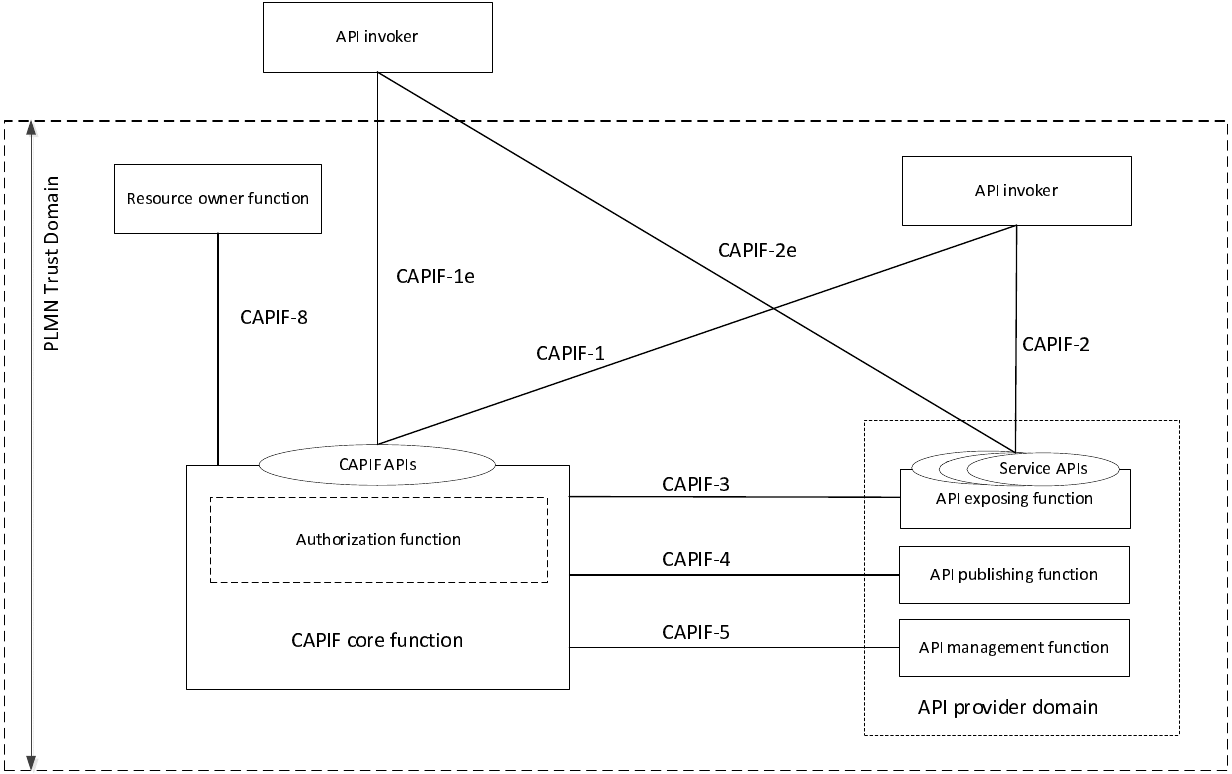
\includegraphics[width=1\linewidth]{figs/capif-architecture.png}
    \caption{High level functional architecture for CAPIF supporting \acs{RNAA}~\cite{ETSI_CAPIF_TS_123_222_V18_4_0}}
    \label{fig:capif-architecture}
\end{figure}


\customparagraph{API Invoker}

The \acs{API} Invoker is typically provided by a third-party application, on a server or \acs{UE}, who has a service agreement with the \acs{PLMN} operator. The \acs{API} Invoker may reside within or outside the \acs{PLMN} operator trust domain and has the following main goal: triggering its onboarding/offboarding and authentication with \acs{CAPIF}, discovering available service \acsp{API} and invoking those \acsp{API} to access network or service capabilities. 

\customparagraph{API Provider}

The \acs{API} Provider represents an entity that owns and exposes \acsp{API} to the \acs{API} Invokers through the CAPIF framework. It provides three different functions: \ac{CAPIFAEF}, \ac{CAPIFAPF} and \ac{CAPIFAMF}.

The \ac{CAPIFAEF} is the service \acs{API} provider and communication entrypoint to the \acs{API} Invokers, handling its authentication and validating the authorization provided by the \ac{CCF} via \acs{JWT}. It is also responsible for logging the service \acs{API} invocations at the \ac{CCF}. The \ac{CAPIFAPF} allows \acs{API} providers to publish their service \acs{API} information to the \ac{CCF} in order to support \acs{API} discovery by \acs{API} invokers. The \ac{CAPIFAMF} lets the \acs{API} provider perform administration of the service \acs{API} including auditing service \acs{API} invocation logs and  monitoring events from \ac{CCF}. It also allows the \acs{API} provider to configure policies to the \ac{CCF}, between other capabilities.

\customparagraph{CAPIF Core Function}

The \ac{CCF} is the core component and acts as the central repository for all published \acsp{API}, controlling service \acs{API} access based on \acs{PLMN} operator configuration policies and handling aspects related to storing (logs provided by the \ac{CAPIFAEF}), auditing, charging and monitoring service \acs{API} invocations. Related to the \acs{API} invoker it is responsible for its onboarding/offboarding, authentication and authorization prior to it accessing the service, as well as publishing, storing and supporting the discovery of service \acs{API} information. In the context of a 4G or 5G system, the \ac{CAPIFAEF} corresponds to the \ac{SCEF} or \ac{NEF} functions.

Lastly, with the goal of \acs{CAPIF} supporting \ac{RNAA} two additional functions are defined: the authorization function and a resource owner function. The former is an internal entity of the \ac{CCF} and interacts with the \ac{CAPIFAEF}, which acts as a resource owner consent enforcement point. The latter interacts with the authorization function via CAPIF-8, which is not specified in the current release of the specification.

\hide{

\later{
\later{TS 33.501}
The security aspects of \acs{CAPIF} supporting RNAA are specified in 3GPP TS 33.122 [12].} \later{The API invoker interacts with authorization function in the CAPIF core function via CAPIF-1/CAPIF-1e.} \later{add diagram and all connections} \later{sequence diagram flow} \later{different authentication mechanisms} \later{add reference to pathway\_towards\_NaaS\_CAMARA.pdf which includes CAPIF}

}


\subsection{TM Forum}
\label{sota:telcoinitiatives:tmf}


\ac{TMF}~\footnote{\url{https://www.tmforum.org/}} is a global aliance composed of telco and tech companies from the connectivity ecosystem with the goal of providing a cooperative framework to collaborate and establish industry-wide standards, best practices and toolkits. These include over 800 organizations, encompassing the top 10 \ac{CSP}s, the three leading hyperscalers, major Network Equipment Providers, as well as a diverse array of vendors, consultancies, and system integrators~\cite{aboutTMF}.

The core element of \ac{TMF}'s approach in achieving its missions is the \ac{ODA}. \ac{TMF} \ac{ODA} advocates for the existence of technology agnostic Open \ac{API}s, collaboratively developed by its members to provide standardized interfaces that streamline digital services across a wide range of domains, such as \ac{IoT} or healthcare. In the telecoms industry, the Open \ac{API} Project plays a crucial role in gathering \ac{CSP}s and solution and technology providers to accelerate the deployment of interoperable telecom solutions, tackling integration and delivery complexity while reducing time-to-market~\cite{openAPIsTMF}.

\ac{TMF} Open \ac{API}s rely on a common API data model that is maintained separately from the API specifications: the \ac{TMF} \ac{SID}. This model, used across the Open Digital Architecture and Open APIs, adresses the \ac{CSP}'s need for shared information definitions and models, establishing a standardized way to represent and organize data for implementing business processes. This business model is independent of platform, language or protocol and helps to identify and categorize business entities important to \ac{CSP}s, reducing duplication and promoting consistency and interoperability. More specifically, business entities can be categorized into the following domains: Market \& Sales, Customer, Product, Service, Resource, Business Partner, Enterprise and Common~\cite{SIDTMF}. Three of these domains are essential and widely used across \acfp{OSS}, such as openslice, and are explored further: the Product, Service and Resource domains.

\hide{
\later{mention relation with BSS and OSS} \later{connect with GSMA and CAMARA (i record some of page of their website mentioning it)}
}

\clearpage
\customparagraph{Product}

A Product represents a tangible or intangible item that enterprises such as \ac{SP}s expose and sell to customers for a profit. It is defined in \ac{SID} through a Product Specification detailing its attributes, methods, relationships and constraints, as perceived by the business user and aligned with what the operator intends to sell at a functional level~\cite{SID-MODELS-v250-TMF}.
% maybe other cites

\customparagraph{Service}

A Service represents internally the underlying technical implementation of a Product, which is offered to customers in a commerce perspective. Services can be categorized into \acfp{CFS}, representing, within an organization's infrastructure, the Product the end-customer acquires (e.g. a music streaming service), and \ac{RFS}, which provide the internal implementations required to support a \ac{CFS} in order to deliver its intended functionalities (e.g. recommendation engine supporting music streaming service). Each Service is defined by a corresponding Service Specification~\cite{SID-MODELS-v250-TMF}.

\hide {

\later{mention Service bundles somewhere}
\later{However, the characteristics' values of the instantiated Service will be specific to each instance.}
\later{Service specification can have multiple other service specifications}

}


\customparagraph{Resource}

Resources are the components that support the provision of Services and therefore the delivery of Products to Customers. These include Physical Resources, such as a router or server, and Logical Resources, such as Virtual Machines, \acp{VNF} or software applications, as well as Compound Resources that aggregate them into a single entity. All three Resource types are instantiated from their respective Resource Specifications, as per the specification~\cite{SID-MODELS-v250-TMF}.


\section{Management and Support Systems} \label{sota:bss-oss-mano}

The telecommunications industry is undergoing a fundamental transformation, with telecom service providers facing significant challenges as traditional networks and services become increasingly converged. Since legacy \acs{IT} systems are unable to meet the requirements of new services and customer demands, \acs{OSS}/\acs{BSS} systems, based on the eTOM framework by \acs{TMF}~\cite{eTOM-TMF}, are adopted to enable service focused operations and improve customer satisfaction. These systems serve as management platforms for telecom operators and their networks, allowing them to capitalize on new revenue streams by delivering new services to customers~\cite{NGOSSEvolutionTelecomSP}.

Their implementation is central to reducing costs and improving operational and organizational efficiency~\cite{NGOSSEvolutionTelecomSP}. By automating operational tasks, \acs{OSS}/\acs{BSS} solutions allow operators to reduce \acs{OPEX} associated with customer and system management~\cite{OSSMobileNetworks}. This is especially relevant as the number of devices connected to the network grows, with scalability heavily relying on its ability to autonomously configure, provision and update devices without impacting the network~\cite{EricsonOSS}. More importantly, the next generation of \acs{OSS}/\acs{BSS} must advance beyond traditional automation to support orchestration and dynamic allocation of network resources, setting as the ultimate goal a zero-touch network completely integrated with an orchestrator~\cite{SurveyOrchestrationOSSNextGenerationNetworks}.

\subsection{Business Support System}

The \acf{BSS} is responsible for the support of business operations at the customer level. It provides communication services to customers, handling customer-facing operations, including ordering, billing and support. These customer-facing services are fulfilled by the \acs{OSS}, which interacts with the underlying network to ensure service delivery through the corresponding back-office tasks~\cite{CommunicationManagamentPlanOSSCaseStudy}. The \acs{BSS} can be decomposed into the following subcategories~\cite{NGOSSEvolutionTelecomSP}:
\begin{itemize}
    \item \textbf{\acf{CRM}:} system responsible for maitaining and retaining the relationship with the customer by identifying and tailoring to its needs. It includes a structured product catalog, allowing for product configuration according to the customer's requirements. It also supports customer service capabilities with generation of quotes, order tracking and trouble ticket management. Additional functionalities in marketing, customer support and partner management are provided too, all centered around the customer with the goal of maximizing customer experience;

    \item \textbf{Billing \& Charging:} handles management of financial interactions with customers, linking revenue to the provided services. Bill Management and settlement functionalities oversee customer data, bill generation and activity tracking, with account analysis being performed for customer and carrier usage (i.e. examines the services consumed by customers and the use of provider resources).
\end{itemize}


\subsection{Operations Support System}

The \acf{OSS} is defined as a group of integrated \acs{HW}/\acs{SW} applications utilized by network operators to guarantee the efficient operation, management, availability and reliability of the \acs{IT} and telecommunications network. Consumer orders flow down through the \acs{BSS} into the \acs{OSS} layer, which performs the necessary arrangements and activation modifications to the network~\citep{OSSMobileNetworks,CommunicationManagamentPlanOSSCaseStudy}. The \acs{OSS} can be subdivided into the following functional modules~\citep{OSSMobileNetworks, NGOSSEvolutionTelecomSP}:

\begin{itemize}

    \item \textbf{Service Fulfillment:} provisions the services offered by the \acs{BSS} to the customer, applying the necessary modifications to the network. This involves integrating services from multiple vendors and coordinating them in an efficient way;

    \item \textbf{Service Guarantees:} concerns the insurance of services to customers. It handles the configuration, creation and activation of services, incorporating \acs{SLA} Management features to monitor the network and service performance;

    \item \textbf{\acf{NEM}:} provides remote connectivity to network devices offering important configuration and monitoring tools. Instead of each device relying on manual command-line operations, the \acs{NEM} maintains a list of the accessible devices to ensure consistency and accelerate task execution. Also referred to as \acf{EMS}, it primarily focuses on the individual device and its existing state;

    \item \textbf{\acf{NMS}:} responsible for the management of the whole network. The \acs{NMS} grants access to \acs{NEM} funcionalities by directly connecting to devices or interfacing to the \acs{NEM}. In combination, they simplify the process of configuring network elements in a controlled manner, providing fault management capabilities to analyse the state of the network and detect network faults, errors and unavailability scenarios. It also offers performance management operations, investigating the network traffic flow to ensure it meets the expected service quality. Additional functionalities for security management and testing should also be included to support service assurance, with the goal of guaranteeing compliance with customer \acsp{SLA}.

\end{itemize}

The \acs{OSS} complements the \acs{BSS} in the delivery of \acs{E2E} \acs{5G} services to customers. While the \acs{BSS} handles customer-facing interactions, the \acs{OSS} manages the underlying network execution. Together, these systems support the operations of telecom operators, allowing implementation of new services and changes effectively, reducing cost and time to market. It also gives operators the ability to meet evolving user demands, by providing subscribers with mechanisms to create and test services in a more flexible way~\cite{EricsonOSS}.

\subsection{OSS/BSS Integration with NFV-MANO} \label{sec:oss:bss:nfv-mano}

The industry's move towards virtualization has fundamentally transformed how networks are managed and deployed. Therefore, \acs{OSS}/\acs{BSS} systems must evolve to accommodate the increased complexity of virtualized network environments, along with a substantial growth in the number of entities under management~\cite{EricsonOSS}.

However, simply extending existing \acs{OSS}/\acs{BSS} models to account for virtualization is not sufficient, as this approach doesn't support the new capabilities and services offered by \acs{NFV}. Instead, to achieve the full benefit of \acs{NFV}, service providers should consider \acs{NFV-MANO} solutions alongside \acs{OSS}/\acs{BSS} integration and management requirements~\cite{ETSI_GS_NFV_MAN_001_V1_1_1}. For this, \acs{ETSI} defines a series of interfaces within its \acs{NFV-MANO} framework, providing a set of \acs{REST} \acs{API} necessary for the integration with \acs{OSS}/\acs{BSS} systems, providing the following benefits~\cite{ETSI_GS_NFV_MAN_001_V1_1_1}:

\begin{itemize}
    \item \textbf{Open and consistent interfaces}, to facilitate automation and self-service operations at service and product level, supporting rapid, agile responses to changing business needs;

    \item \textbf{Adaptive automation}, with service usage driving on-demand resource requirements and dynamically allocating the necessary resources and services in real time;

    \item \textbf{Orchestration}, leveraging policies (and other mechanisms) to guide decisions and perform system changes;

    \item \textbf{Personalized services}, easily configurable by the operator, end-user or network resource layers to address individual customer preferences and requirements;

    \item \textbf{Technology-driven innovation}, characterized by rapid development, continuous integration, deployment and experimentation, according to business and service operations agility.
\end{itemize}
\section{Testbed Implementations} \label{sec:testbeds:main}


With the goal of developing, testing and validating network-aware applications and services, research initatives rely on experimentation platforms, commonly referred to as testbeds. This experimentation facilities provide access to network resources through virtualized \acs{5G} infrastructure, allowing third parties, such as \acsp{SP}, \acsp{SME}, vertical stakeholders or even the research community to experiment with solutions tailored to specific industry requirements~\cite{ICT-41-2020}. Such platforms abstract the complexities of managing the underlying infrastructure, allowing participants to focus on the design, implementation and evaluation of their own applications, rather than being preoccupied by the provisioning and operational details of the network.

The following section will delve into the details of the testbeds utilized in the literature for validating network-aware systems. Subsection \ref{sec:testbeds:5GC} performs an overview of the various components that tipically constitute testbeds or testing environments, highlighting the diversity of components and setups present in the literature. Then, Subsection \ref{sec:testbeds:5GC:5GC}, examines these testbeds regarding its network exposure capabilities, including adherence to key telecom standardization initiatives, such as CAMARA, \acs{CAPIF} and \acs{TMF} Open \acsp{API}. Lastly, the combined information of the researched testbeds and validation environments, including both the configuration setup and adherence to telecom standardization initiatives is summarized in Table \ref{tab:testbeds:description}.


\subsection{Testbed Architecture and Configurations} \label{sec:testbeds:5GC}

The analyzed testbeds follow a common architectural approach for supporting programmability and exposure of network capabilities, with their core modules being summarized in Table \ref{tab:testbeds:description}. At the center, a \acs{5G} core network forms the backbone of the \acs{5G} system, with implementations ranging from open-source projects, such as Open5GS, Free5GC, \acs{OAI} to commercial solutions, such as Amarisoft, Nokia, and Huawei. Then, the core network connects to the \acs{RAN}, via the transport network, for access to the end devices through \acs{gNB} base stations that may be deployed either as a physical component (e.g. \acs{OAI} \acs{RAN}, Ericsson and Huawei gNodeBs) or simulated software environments, such as UERANSIM.

To promote flexibility and reproducible results, testbeds heavily rely on virtualization and orchestration technologies, with most testbeds leveraging containerization platforms like Kubernetes. \acf{VM} environments are also common utilizing solutions, constructed via OpenStack and VirtualBox.  Moreover, \acs{MANO} solutions compliant with \acs{ETSI} \acs{NFV} standards are also present to manage network functions and services, with \acf{OSM} being widely utilized.


Regarding network capability exposure, an analysis was performed covering the various network exposure mechanisms across the various testbeds, namely the \acs{NEF} implementations discussed in Section \ref{exposure:NEFimplementations}, as well as adherence to the telecom standardization initiatives mentioned in Section \ref{sota:telcoinitiatives} (i.e. CAMARA, \acs{CAPIF}, \acs{TMF} Open \acsp{API}). A detailed analysis of the exposure mechanisms constructed utilizing this interfaces is provided in the following section.

\hide
{

Regarding physical implementations, multiple testbeds utilize commercial solutions for the \acs{RAN}. \citet{OnDemandNetworkQoSAdaptation} deploy their work on the experimetal infrastructure of the Dutch National \acs{6G} testbed (FNS), which includes a \acs{B5G} core and an Ericsson \acs{gNB} with outdoor antennas. In Aveiro, several contributions rely on the 5GAIner testbed, an Huawei commercial-grade \acs{5G SA} Network (3GPP release 17), featuring Huawei \acs{5G} New Radio cells suitable for both outdoor and indoor scenarios~\cite{5GAIner}. Alternatively, enumerous testing environments opt to simulate both the \acs{UE} and the \acs{gNB} by using UERANSIM~\citep{LoadBalancingConnectedVehicleServices,CloudEnabledDeployment5GN,DesignAndEvaluationNetworkDigitalTwin,NSSFfunction6GNetworksMLOPS}, an open source \acs{5G} \acs{UE} and \acs{RAN} simulator. However, UERANSIM does not actually implement \acs{5G} radio protocols bellow the \acs{RRC} layer, simulating it with a \acs{UDP}-based \acf{RLS} protocol to connect the \acs{gNB} and \acs{UE}, which may introduce disparities in the testing process providing unrealistically high throughput and overly optimistic latency due to the absence of physical layer processing~\cite{EvaluatingOpenSource5GSATestbeds}.

For experiments requiring real \acs{RF} transmission and reception, full \acs{RAN} implementations such as \acs{OAI} can be used, as it supports physical layer operations and is compatible with \acs{USRP} hardware. \citet{ExplorationNWDAFDevelopmentArchitecture6G} combines a Open5GS core and an \acs{OAI} \acs{RAN} with \acs{USRP} hardware to simulate real-world scenarios with a \acs{gNB} and \acs{UE}. As the \acs{OAI} also provides a 3GPP compliant \acs{OAI} \acs{5G} core (\acs{SA}), other authors utilize a full \acs{OAI} \acs{5G} system, with both the \acs{RAN} and \acs{5GC}~\cite{BenefitsCaveatsQoDNetworkAPIsVideoStreaming}. 

Another approach, widely used in the literature, correspond to network emulators. In this field, commercial offerings by Amarisoft are the most prominent in the literature, with multiple versions of Amarisoft Callbox being employed for testing of the \acs{RAN} and/or the \acs{5G} \acs{CN}~\citep{AdvancingPredictiveSecurity,PerformanceComparisonNWDAFSecurity}. This may include \acs{5G SA} setups incorporated with \acs{SDR} elements and \acfp{RRH} for enhanced coverage~\cite{VirtualOnBoardUnitMigration}. Additionally, \acsp{UE} can also be emulated via Amarisoft's Simbox and connected to \acsp{gNB} from Amarisoft Callbox~\cite{DemoOnDemand5GEdgeVerticalsViaThirdPartyUPF}.

}


\subsection{Network Exposure Interfaces} \label{sec:testbeds:5GC:5GC}

The integration of network exposure interfaces within testbed implementations demonstrates varying degrees of architectural maturity and standardization compliance. This section expands on the configuration of the testbeds provided in Table \ref{tab:testbeds:description}, with particular emphasis on their configuration for exposing network capabilities. This may include the implementation of \acs{NEF}, CAMARA and \acs{TMF} \acsp{API}, as well as secure service exposure through \acs{CAPIF}.

\citet{DesignAndEvaluationNetworkDigitalTwin} implements a \acf{NDT} platform with Open5GS of a physical \acs{5G} testbed built with Amarisoft, enabling closed-loop automation and \acs{AI}/\acs{ML} driven network intelligence. With this goal, the authors repurpose the Katana Slice Manager, developing an \acs{NDT} orchestrator responsible for the provisioning, synchronization, and automation of \acs{NDT} instances. More specifically, Katana is integrated with \acs{OSM} to manage the deployment of Open5GS \acs{NSD}/\acs{KNF}, guaranteeing they are instantiated within the Kubernetes environment~\cite{videoNDTDemokritos}. The system utilizes Prometheus for managing the collection, storage, and retrieval of network telemetry and simulation data, with visual analytics being obtained via Grafana. Although the authors specify an \acs{NDT} framework suitable for \acs{B5G}/\acs{6G} networks, it is not addressed the exposure of services suitable for third parties, with no references to either \acs{NEF} or CAMARA \acsp{API}.

In contrast, \citet{BenefitsCaveatsQoDNetworkAPIsVideoStreaming} utilizes the CAMARA \acs{QoD} \acs{API} to improve the \acs{QoE} of video streaming scenarios in a network with challenging conditions. This is achieved through a cache server that interfaces with the CAMARA \acs{QoD} \acs{API} to request temporary bandwidth boosts. However, the underlying implementation relies on low-level xApps deployed at the \acs{RIC}, a layer above the \acs{RAN}, with no references to either \acs{NEF} or other \acsp{NF} of the \acs{5GC}. This approach promotes tighter coupling between the application and the \acs{RAN} specific implementation, not taking advantage of the exposure and abstraction layer provided by the \acs{NEF}.

There are other approaches for offerring CAMARA services, incorporating additional abstraction layers that decouple the service logic from the underlying \acs{RAN} implementation, focusing for instance in \acs{TMF} \acsp{API}~\cite{CAMARAaaSdemo}. The introduced \acs{CAMARAaaS} approach integrates CAMARA with \acs{TMF} \acsp{API} to offer a standardized interface to manage \acs{5G} resources, assuming network services can be exposed through \acs{TMF} \acsp{API}. More specifically, it showcases how the \acs{QoS} of an \acs{UE} can be controlled with the CAMARA \acs{QoD} Provisioning \acs{API}. In practice, it introduces a middleware layer to translate the CAMARA \acs{API} requests into operations from the \acs{TMF} 638 - Service Inventory Management \acs{API}, included in the suit of \acs{TMF} \acsp{API} offered and fulfilled by the \acs{OSL} \acs{OSS}. 

\citet{DynamicQoSAdaptationviaExposedServiceAPIs} extends on this use case by detailing end-to-end specifications for the implementation of two CAMARA services, the Device Location and \acs{QoD} \acsp{API}, in the context of a vehicular remote monitoring digital twin use case. The CAMARA \acsp{API} are exposed by the \acs{B5G} core at the \acs{AF} layer, enabling device location notifications and on-demand \acs{QoS} requests for the selected \acsp{UE}. By combining these \acsp{API}, a \acs{V2X} server can automatically request a high-priority \acs{QoS} profile whenever the Device Location \acs{API} indicates a vehicle has entered a congested geographical area, solely through the \acs{AF} layer without directly interacting with underlying network functions. This layer converts the requests to internal \acs{3GPP} procedures required by the \acs{NEF}, which coordinates with the relevant \acsp{NF}, i.e. the \acs{PCF} and the \acs{AMF} for the \acs{QoD} and Device Location \acsp{API}, respectively. This is especially relevant as even lower-level interactions, between the \acs{AMF} and the \acs{gNB} for obtaining the actual \acs{NGAP} Location Reports, get abstracted.

With respect do dynamic \acs{QoS} adaptation via exposed \acsp{API}, \cite{NextGenConnectivityDynamicQoS} proposes two EdgeApps, the Situational Awareness EdgeApp and the Quality Awareness EdgeApp, responsible for requesting modifications in the \acs{QoS} (requesting a slice profile with higher bandwidth) upon detection of special events using geofencing (e.g. entering higher \acs{QoS} area) and antecipating potential network deterioration, respectively. It differs from the previous work, by introducing Nokia's \acf{NaC} solution to expose the CAMARA \acs{QoD} and Device Location \acsp{API}. The \acs{NaC} \acs{SDK} is integrated directly into the edge network applications to create real-time events and trigger changes in the \acs{QoS}, which are fulfilled by the \acs{NaC} backend services through the \acs{NEF} into the Telenet \acs{5G} Core, also based on Nokia technology. Nonetheless, the details of the underlying implementation at the level of the \acs{5G} core are not specified, with the solution being tighly coupled to the proprietary Nokia \acs{NaC}.

A common limitation across all the previous analysed implementations is the lack of \acs{CAPIF} support for secure discovery, exposure and consumption of northbound \acsp{API}, provided by \acs{NEF} and/or CAMARA. \cite{PathwayNaaSCAMARA} presents a solution that incorporates \acs{CAPIF} to publish CAMARA \acsp{API}, and policy their exposure to third party applications. It leverages the CAMARA \acs{QoD} \acs{API} to create a traffic management application to be used by third parties (e.g. streaming platform), modifying the \acs{QoS} profile (bandwidth and latency) associated to individual \acsp{UE} to prevent performance degradation. The \acs{QoS} modifications are abstracted by CAMARA and enforced by the \acs{NEF}, which interfaces with the \acs{5GC} via its \texttt{AsSessionWithQoS} \acs{API}. This corresponds to the most complete test environment, regarding the exposure of network capabilities, incorporating \acs{NEF}, CAMARA and \acs{CAPIF} in the final solution, as shown in Table \ref{tab:testbeds:description}.

\begin{table}[ht]
\centering
\tiny
\renewcommand{\arraystretch}{1.3} % Increase row height
\rowcolors{2}{gray!15}{white}     % Alternating row colors
\caption{Testbed Implementation Configurations}
\label{tab:testbeds:description}
\begin{tabular}{p{2cm} p{2cm} p{2cm} p{2cm} p{1.4cm} p{1.4cm} p{1.4cm} p{1.4cm}}
\toprule
\textbf{Source} & \textbf{\acs{5G} Core} & \textbf{\acs{5G} \acs{RAN}} & \textbf{Virtualisation / Orchestration} & \textbf{\acs{NEF}} & \textbf{CAMARA} & \textbf{\acs{CAPIF}} & \textbf{\acs{TMF}} \\
\midrule
Advancing Predictive Security~\cite{AdvancingPredictiveSecurity} & Amarisoft Classic, NCSRD-DS-5GDDoS testbed. & Amarisoft Callbox Mini and 2 cells - Amarisoft Classic. & Not specified. & NO. & NO. & NO. & NO. \\
Exploration of \acs{NWDAF} Development Architecture~\cite{ExplorationNWDAFDevelopmentArchitecture6G} & Open5GS. & \acs{OAI} using \acs{USRP} B210. & Kubernetes. & NO. & NO. & NO. & NO. \\
Network Slice Selector in \acs{IoT} Services~\cite{NetworkSliceSelectorIoT} & OpenAirInterface, GNS3 emulator. & \acs{OAI} gNodeB (CUPS Ubuntu). & Kubernetes (openair-k8s), \acs{OSM}, GNS3. & NO (\acs{NWDAF} focus). & NO. & NO. & NO. \\
Cloud-Enabled Deployment of \acs{5G} Core Network~\cite{CloudEnabledDeployment5GN} & Open5GS. & UERANSIM (\acs{gNB} and \acs{UE}). & VirtualBox, Debian \acsp{VM}. & Custom Quasi-NEF in Python. & NO. & NO. & NO. \\
Dynamic QoS Adaptation Via Exposed Service \acsp{API}~\cite{DynamicQoSAdaptationviaExposedServiceAPIs} & TNO \acs{B5G} Core (Open5GS based), TNO Hague lab, Rel-17. & Ericsson gNodeB, \acs{SA} mode. & OpenStack \acsp{VM}. & YES (TNO \acs{NEF}). & \acs{QoD}, Device Location. & NO. & NO. \\
Load Balancing in Connected Vehicle Services~\cite{LoadBalancingConnectedVehicleServices} & Free5GC, distributed edge servers, v3.3.0. & UERANSIM (\acs{UE} and \acs{gNB}). & Ubuntu \acsp{VM}. & Custom Go implementation. & Traffic Influence \acs{API}. & NO. & NO. \\
An Automated Testing and Orchestration Framework~\cite{AutomatedTestingOrchestrationFramework} & Huawei \acs{5G} \acs{SA} Core, 5GAIner infrastructure, Rel-17. & Huawei \acs{5G} New Radio cells. & \acs{OSM}, Kubernetes, OpenStack. & NEFSim~\cite{NEFSimMediaNetLabGithub}. & NO. & NO. & YES (\acs{OSL}). \\
Virtual On-Board Unit Migration~\cite{VirtualOnBoardUnitMigration} & GAIA \acs{5G} (Amarisoft), University of Murcia. & Amarisoft macro cells. & OpenStack (Rocky), \acs{OSM}. & NEFSim~\cite{NEFSimMediaNetLabGithub}. & NO. & NO. & NO. \\
Next-Gen Connectivity: Dynamic \acs{QoS} Optimization~\cite{NextGenConnectivityDynamicQoS} & Telenet \acs{5G} \acs{SA} (Nokia), Antwerp VITAL-5G testbed. & Antwerp gNodeB units. & OpenStack, \acs{OSM} (VITAL-5G). & YES (with Nokia \acs{NaC}). & \acs{QoD}, Device Location. & NO. & NO. \\
On the benefits and caveats of exploiting \acs{QoD}~\cite{BenefitsCaveatsQoDNetworkAPIsVideoStreaming} & OpenAirInterface \acs{5G} Core. & OpenAirInterface \acs{5G} \acs{RAN}. & Not specified. & NO (uses \acs{RIC} directly). & \acs{QoD}. & NO. & NO. \\
On-Demand Network QoS Adaptation~\cite{OnDemandNetworkQoSAdaptation} & TNO \acs{B5G} Core, Dutch National \acs{6G} testbed (FNS), Rel-17. & Ericsson gNodeB, Rel-16. & TNO research cloud. & YES (Internal TNO \acs{B5G}). & \acs{QoD}, Performance Metrics. & NO. & NO. \\
Design and Evaluation of a \acs{NDT}~\cite{DesignAndEvaluationNetworkDigitalTwin} & Open5GS, NCSR Demokritos \acs{5G}+ testbed. & UERANSIM. & \acs{NDT} Katana Orchestrator. & NO. & NO. & NO. & NO. \\
\acs{NSSF} Function in \acs{6G} Networks Based on MLOps~\cite{NSSFfunction6GNetworksMLOPS} & Not specied, containerised. & UERANSIM simulator. & Kubernetes (K8s cluster). & NO (NSSF/NWDAF focus). & NO. & NO. & NO. \\
Performance Comparison of NWDAF-Based Security~\cite{PerformanceComparisonNWDAFSecurity} & Amarisoft Callbox Classic, "\acs{5G}-in-a-box" lab platform. & Amarisoft (\acs{SA} mode). & NO. & NO. & NO. & NO. & NO. \\
Offering CAMARA APIs as a Service - Demo~\cite{CAMARAaaSdemo} & Huawei \acs{5G} Core, 5GAIner testbed, Rel-17. & 5GAIner New Radio cells. & Kubernetes (\acs{OSL}'s CRIDGE). & NO. & \acs{QoD} Provisioning \acs{API}. & NO. & YES (\acs{TMF} 638, \acs{OSL}). \\
Pathways towards network-as-a-service~\cite{PathwayNaaSCAMARA} & \acs{SA}, Release 15. & single gNodeB. & containerized. & YES. & \acs{QoD} \acs{API}. & YES. & NO. \\
Experiences and challenges on testing~\cite{ExperiencesChallengesTestingValidatingNetworkAware} & Patras5G Core, Patras5G testbed. & AW2S \acs{gNB}. & containerized and virtualized. & NO. & NO. & NO. & YES (\acs{OSL}). \\
Pushing the Boundaries of Scalable 5G Core~\cite{pushingBoundariesScalable5GCN} & Open5GS. & Not specified. & Kubernetes cluster. & custom microservices \acs{NEF}. & NO. & YES (OpenCAPIF). & NO. \\
Optimizing \acs{3GPP} \acs{5G} \acs{NEF} Integration~\cite{optimizing5GNEFIntegrationThroughNEFandUPF} & Not specified. & General Access Nodes. & Not specified. & YES (custom \acs{NEF}). & \acs{QoD} \acs{API}. & NO. & NO. \\
Capability Exposure Vitalizes \acs{5G}~\cite{CapabilityExposureVitalizes5GNetwork} & \acs{5G} Core Trial, Hangzhou site. & \acs{5G} \acs{RAN}. & Not specified. & YES (custom). & NO. & NO. & NO. \\
Data Collection Using \acs{NWDAF}~\cite{DataCollectionUsingNWDAF5GCN} & \acs{5G} Core, Linux-based testbed. & Not specified. & Linux \acs{VM} and Namespaces. & NO. & NO. & NO. & NO. \\
\acs{TMF} Open Digital Architecture for \acs{5G} Service Orchest.~\cite{TMFOpenDigitalArchitecture5GServiceOrchestration} & Huawei \acs{5G} \acs{SA} Core, 5GAIner, Rel-17. & Huawei \acs{5G} New Radio cells. & \acs{OSM}, Kubernetes, OpenStack. & NO. & \acs{QoD} Provisioning \acs{API}. & NO. & YES (\acs{OSL}). \\
\bottomrule
\end{tabular}
\end{table}



\section{Testing \& Validation} \label{sec:testingandvalidation}

The telecommunications sector is characterized by stringent \acs{QoS} and performance requirements, inherent to carrier grade networks. With the industry move towards the cloud, it becomes essential to conduct testing procedures to ensure the operation and dimension of cloud-based network elements (i.e. \acs{VNF} and \acs{CNF}) and provide network services that can benefit from cloud technology with slicing and scaling mechanisms. This encompasses laboratory and field testing scenarios, as well as active monitoring and collection of metrics and \acsp{KPI} (e.g. resource utilization) to enable analysis of traffic patterns, relevant for predictive solutions, and closed-loop network automation~\cite{CapacityPerformanceTestMethodsCloudNF}.

\subsection{Data Collection and Analysis via NWDAF}

An important area of research corresponds to the development of \acs{ML} \acs{NWDAF} models for predicting \acs{DDoS} attacks or implementing autoscaling tecniques to dynamically adjust network resources in response to high traffic conditions. \citep{UserTerminalsAsAttackers, AdvancingPredictiveSecurity} utilize an annotated dataset to detect \acs{DDoS} attacks collected from a \acs{5G} testbed. The studies focuses mainly on the validation of the \acs{ML} algorithms and analysis of the traffic profile of the benign (using Skype and Youtube) and malicious \acsp{UE} (performing the various \acs{DDoS} attack types). Despite specifying that there are a total of nine \acsp{UE} (five of them malicious), each attributed to a specific cell, the underlying functional implementation of traffic generation and data collection are not specified. However, the set of features collected, from the various \acsp{NF}, and utilized by the algorithm constitute key insights for such prediction endeavors. \citet{PerformanceComparisonNWDAFSecurity} address the same use case, distinguishing between Control Plane and Data Plane \acs{DoS} scenarios. In the first scenario, anomalous behavior was characterized by very quick and frequent association-deassociation of \acsp{UE}, to flood the network control plane, whereas the second scenario performed the \acs{DoS} attack utilizing the hping tool deployed in the \acs{UE}. The data collection process is implemented through a pipeline that periodically issues asynchronous, non-blocking requests to WebSocket \acsp{API}, provided by the \acs{5G} platform powered by Amarisoft Callbox Classic. The collected metrics include downlink and uplink bitrates, transmission and error counts, session management statistics and \acs{UE} registration records. Nonetheless, the study lacks validation procedures to evaluate the correctness of the data collection process under real-world conditions.

In contrast, \cite{DataCollectionUsingNWDAF5GCN} validates a custom \acs{NWDAF} implementation and the coherence of the metrics collected (i.e. comparison of application-level metrics versus metrics collected by the \acs{NWDAF}), according to generated traffic, within a \acs{5G} system in a Linux-based \acs{VM} testbed. The testbed is constituted of a \acs{RAN} \acs{VM} connecting a \acs{UE} \acs{VM}, containing all the \acsp{UE}, to a intermediary \acs{UPF} (I-\acs{UPF}), which in turn connects to an anchor \acs{UPF} (A-\acs{UPF}) that hosts the server-daemon pairs for the \acsp{UE}. The \acs{NWDAF} metrics are obtained at the I-\acs{UPF} for uplink data volume and \acs{RTT}, while the A-\acs{UPF} measures the downlink data volume. In order to generate traffic, a custom traffic loader was developed in Go and Bash, using iPerf3 v10 to produce synthetic traffic based on predefined \acs{YAML} configuration files with configurable uplink and downlink traffic models for \acs{TCP} or \acs{UDP}. This tool is composed by two components: a simulated \acs{UE} and a corresponding server-side daemon that receives (uplink) or sends (downlink) the requested byte stream. By combining it with isolated network namespaces with different \acsp{IP}, it's possible to synthesize traffic with \acs{PDU} session granularity, between different source \acsp{IP} and the network, representing the \acsp{UE} served by a network slice. With this setup, four different traffic profiles are configured to test the \acs{NWDAF}: \acs{TCP}-Long, \acs{TCP}-Short, \acs{UDP}-\acs{CBR}, \acs{UDP}-\acs{VBR} and a combined profile incorporating them all. The average bit rate (throughput) of these traffic profiles is then compared to the \acs{NWDAF}'s, corroborating the collected metrics. To validate latency measurements, the \acs{NWDAF} statistics were compared against the ping result among the \acsp{UPF} serving a slice with variable background conditions. In this case, the traffic generation process was achieved manually, for the sake of validating the collection of data by the \acs{NWDAF}. However, ideally this would be achieved automatically without human intervention, through continous validation of the \acs{NWDAF} metrics in real time or, at least, through the use of dedicated validation platforms that can automate traffic generation and other related procedures.

Despite detailing the collection of metrics, the previous \acs{NWDAF} implementation is limited to the \acs{UPF} and operates at a low level within a Linux-based \acs{VM} testbed, not realistic for real world environments. By comparison, \cite{ExplorationNWDAFDevelopmentArchitecture6G} presents a full architecture for the \acs{NWDAF} with data collection and management, and model training and management components, for a vertical scaling use case within a testbed composed by a Open5GS Kubernetes \acs{CN} (with \acs{AMF}, \acs{SMF} and \acs{UPF}) and \acs{OAI} integrated with \acs{USRP} hardware. Two \acsp{UE} are connected to the \acs{CN}, with traffic load being generated by transmitting data packets between them using the iPerf tool. During the experiment, real-time data is collected via Prometheus from the \acs{AMF}, \acs{SMF} and \acs{UPF} to monitor the experiment and trigger \acs{UPF} vertical scaling actions based on \acs{UPF} \acs{CPU} usage. The analysis of this data corroborated the increase of \acs{AMF}/\acs{SMF} traffic upon \acs{UE} connection and of the number of N4 sessions due to data transmission. Lastly, the \acs{UPF} traffic values remained at a constant level showcasing  successful communication between devices, with intensive data transmission triggering \acs{UPF} scaling across three different \acs{ML} models with a lower response time than a 70\% \acs{CPU} threshold based strategy.


\subsection{Network Applications} \label{sec:testingandvalidation:netapps}

The development of Network Applications needs to be accompanied by testing procedures, leveraging monitoring stacks and collected metrics to validate usage scenarios in real testbeds. This section reviews the testing methodologies and validation mechanisms reported in the literature, focusing on how they're used to assess and demonstrate the feasibility of some of the use cases discussed throughout this document.

In the Section \ref{sec:testbeds:5GC:5GC}, it was presented a dynamic \acs{QoS} adaptation scenario based on the CAMARA Device Location and \acs{QoD} \acsp{API}, in the context of a vehicular remote monitoring digital twin use case~\cite{DynamicQoSAdaptationviaExposedServiceAPIs}. A testing experiment is performed to showcase the dynamic \acs{QoS} modifications at a designated geographical area, represented by a cell ID. As only a single \acs{gNB} is available, radio cell changes are emulated by periodically modifying the cell ID of connected \acsp{UE} at the \acs{AMF}, simulating movement between different geographical areas. Two \acsp{UE} continously generate iperf \acs{TCP} uplink traffic, at a combined data traffic of 10 Mbit/s. The \acs{V2X} service subscribes to location updates for one of the \acsp{UE} and upon entering a specific area (the north cell) it enforces a \acs{QoS} profile (via the CAMARA \acs{QoD} \acs{API}) with absolute priority of the selected \acs{UE}'s data flow over other traffic, automatically removing it when the \acs{UE} leaves. This process is performed 200 times to collect statistically relevant measurements. The data collection and analysis is achieved through the use of Prometheus and Grafana, at the level of the server infrastructure (OpenStack). In result, the \acsp{UE} compete equally in the absence of any high-priority \acs{QoS} profile, with each \acs{UE} generating roughly 5 Mbit/s of throughput, as opposed to the selected \acs{UE} displaying 9 Mbit/s of throughput when the \acs{QoS} profile is enforced on the north cell. The latency derived of the combined usage of both \acsp{API} was also measured between the network detecting a location change (with a \acs{NGAP} location report at the \acs{AMF}) and the \acs{QoS} profile being confimed at the \acs{gNB}, resulting in 50th percentile latency of 255.0 ms, 90th percentile of 282.8 ms, 95th percentile of 290.3 ms, and 99th percentile of 337.0 ms. These latency values essentially represent an order of magnitude of the overall latency, being dependant on the specific implementation and geographical area, and could be further reduced by employing predictive models that antecipate when the \acs{QoS} profile shoud be applied.

A similar approach is followed in a tele-operated driving context, leveraging the same \acs{QoD} \acs{API} and a performance metrics \acs{API} to provide subscribers with periodic performance data for a device. The tele-operation service is assigned the high priority \acs{QoS} profile, depending on the test case, whereas the general-purpose default \acs{QoS} profile is assigned to a \ac{UE} that continuously sends background iperf \acs{TCP} traffic up to the maximum achievable uplink throughput of roughly 30 Mbit/s. Similarly to the previous study, when the \acs{QoD} was disabled the \acs{UE} competed for the bandwidth reaching an higher throughput (15 Mbit/s compared to 10 Mbit/s achieved by the vehicle) and resulting in a lower average frame rate of 15 \acs{FPS} and an \acs{E2E} network latency of up to 1200 ms. Setting the high priority \acs{QoS} profile (manually through a \acs{GUI}), stabilized the \acs{FPS} and \acs{E2E} latency at substantially lower values, as the data traffic coming from the vehicle has priority over the background traffic. The metrics collection process relies on an \acs{NWDAF} implementation leveraging the testbed Prometheus exporter for retrieving \acs{UPF} data, with the \acs{E2E} latency corresponding to the total delay between a network packet being sent by the vehicle and received at the remote station.

Both previous approaches validate their use cases demonstrating how throughput varies under the applied \acs{QoS}. However, this validation approach is inherently limited to use cases focused on \acs{QoS} management. \cite{VirtualOnBoardUnitMigration} deviates from this use case and validates the automatic migration of a v\acs{OBU} between \acs{MEC} domains as a vehicle moves between \acs{5G} cells. The implementation was tested in two different parts: first in a controlled indoor lab the \acs{OBU} interacts with a \acs{NEF} Emulator to subscribe to cell change events triggered by a simulated device on a predefined path, followed by an outdoor experiment where an actual vehicle (with an \acs{OBU}) travels between coverage areas to trigger a physical handover in an outdoor \acs{5G} network. Openstack was the virtual infrastructure manager used, with \acs{OSM} being chosen as the orchestrator to manage the dynamic deployment of the v\acs{OBU} \acs{5G} Network Application. In both test cases, the v\acs{OBU} migration to a new \acs{MEC} domain was successful, with the latter being corroborated by a spike on \acs{CPU} usage of the Openstack compute node located in the given \acs{MEC} domain the migration occured to.


\subsubsection{Testing Pipelines} \label{sec:pipelines}

Despite validating the basic functionality of the implementations for each case, there is still insufficient adherence to testing pipelines with automated processes for provisioning each of the components present in the respective validation scenario. Instead most testing procedures still rely on low-level scripts or manual workflows to evaluate their applications. Therefore, in this section it's performed an overview of the various validation procedures, with different levels of automation, present in the literature.

\citet{ExperiencesChallengesTestingValidatingNetworkAware} explore the validation of network-aware \acs{PPDR} \acs{XR} applications in the Patras\acs{5G} testbed. To this end, \acs{OSL} was used as the \acs{OSS}, being responsible for provisioning and orchestrating the depoyment of all components to provide a private \acs{5G} network for testing. This includes any appropriate service that's available through the \acs{OSL} service catalog, including \acs{5G} network capabilities and \acsp{gNB}. Telemetry and monitoring tools are integrated in the Patras\acs{5G} testbed by using Prometheus, providing metrics about the \acs{RAN}, along with additional metrics obtained via custom data collectors. Then, for each of the three tested \acfp{UC}, \acsp{VM} were provisioned according to their specific requirements (specs, network access, traffic requirements, \acs{GPU} access). Such \acsp{VM} also include simulated \acsp{UE}. During the lab trials of each \acs{UC} metrics for bandwidth consumption and application latency were measured. The testing methodology combined remote testing for \acs{UC} owners to install and configure their applications on the \acsp{VM}, while testbed personnel managed the network infrastructure and any physical devices, followed by physical testing mostly related to including physical \acs{AR}/\acs{VR} equipment in the testing process. Consequently, despite usign \acs{OSL} for orchestration and provisioning, the process remains partially automated, requiring a certain level of manual configuration for tasks such as the installation and setup of applications in the provisioned \acsp{VM}.

There are more complete solutions within the literature, including a full framework to orchestrate, test, and validate network applications based on the 5GASP project~\cite{AutomatedTestingOrchestrationFramework}. This framework addresses the full workflow of (i) onboarding the network application, (ii) their orchestration, and (iii) the orchestration of the tests to be performed to the network application. The network application and its testing processes are packaged as a bundled service within \acs{OSL}, which also includes a Network Slice Template (based on \acs{GSMA}'s \acs{GST}) to allow testing the application under specific network conditions. For orchestrating the network application, \acs{OSL} interacts with \acs{OSM} via the interface SOL005, supporting the deployment of network applications in both Openstack and Kubernetes. The test cases are defined by a 5GASP Testing Descriptor, in \acs{YAML}, and carried out via the Robot Framework, which automatically produces report and log files in \acs{HTML}. Based on this blueprint, a \acs{CI} Service Testing Orchestrator orchestrates the testing processes, dynamically generating pipeline configuration files and submitting them to Jenkins \acfp{TEA} for execution. After collecting and running all test cases, the \acsp{TEA} aggregate the testing outputs and forward them to the \acs{CI} Service, which creates a visual testing reporting on \acs{OSL} for testers. Regarding monitoring, the computing and resource usages of network app components are scraped from Openstack and Kubernetes using Prometheus, and visualized via Grafana, with measurements on the \acs{5G} resources consumed by each network app being obtained through a man-in-the-middle monitoring switch between the \acs{NFVI}/\acs{CNI} and the \acs{5G} system. This switch handles all interaction between the network applications and the \acs{5G} \acsp{UE}, allowing extensive \acs{KPI} validation and monitoring of throughput, \acs{RTT}, jitter and packet loss percentage. The testing framework was applied in the validation of 11 different network applications across 4 different agnostic testing scopes: \acs{5G} readiness, Security \& Privacy, Performance \& Scalability and Availability \& Continuity.

Although offering a comprehensive DevSecOps testing solution, the framework does not follow a phased methodology that ensures each deployed artifact operates as expected before progressing to deploy additional artifacts. In this context, the following approach extends on the previous work by designing a multistage testing pipeline to support the design, orchestration, and lifecycle management of \acs{5G} resources, such as network slices, and applications~\cite{TMFOpenDigitalArchitecture5GServiceOrchestration}. Similarly to the previous approach, the \acs{OSL} corresponds to the entrypoint of the framework, providing \acs{TMF}-aligned data models and \acsp{API}. \acs{GSMA}'s \acsp{NEST} are mapped into \acs{OSL} services to offer configurable network slices tailored to specific use cases. Once ordered from the \acs{OSL} Service inventory, it is converted  into actionable data models to be consumed by an orchestrator capable of provisioning the network slice, which then becomes accessible in \acs{OSL} for full lifecycle management. This approach is also adopted for the provisioning of other \acs{5G} resources, such as an \acs{UE}. Regarding orchestration, the \acs{OSL} provides interfaces for orchestrating \acs{NFV} (using \acs{OSM} through \acs{ETSI} SOL005) and containerized (using kubernetes through CRIDGE component) applications. To offer monitoring components and simplified CAMARA \acsp{API} for the management of \acs{5G} resources and applications, \acs{TMF} services are again utilized, deploying Prometheus/Grafana monitoring bundles via \acs{OSM} and CAMARA \acsp{API} through Kubernetes.

For performing the testing procedure, the previous DevOps testing solution~\cite{AutomatedTestingOrchestrationFramework} is integrated via the \acs{TMF} 653 \acs{API} (Service Test Management) to support a multi-step approach with the following steps: (i) onboard/design/configuration of \acs{5G} resources and application, (ii) order network slice provisioning, (iii) order \acs{5G} \acs{UE} provisioning, (iv) validate network slice (as per the \acs{SLA}), (v) order application, (vi) validate application, (vii) order monitoring stack, (viii) order CAMARA \acsp{API}, with the service becoming ready for use. The provisioning of network slices and \acsp{UE} was achieved by using a proprietary network slicing \acs{API} from 5GAIner. A computer vision application for monitoring an assembly line, which leverages a CAMARA \acs{QoD} Provisioning \acs{API} to support diverse video streaming requirements, was tested under this pipeline. The first validation step evaluates the network slice capabilities using the provisioned \acs{UE} in regards to throughput, latency, packet loss, jitter, and power consumption, with iPerf3, ping, and a custom Python script being used to measure the latency between the \acs{5G} \acs{UE} and the application. The second validation stage executed 2 custom test cases using a healthcheck to verify that the application's \acs{AI} model is running and it can consume video streams from the \acs{5G} \acs{UE}. 

\hide{
\later{se tiver tempo (não vou ter xD): NSSF Function in 6G Networks Based on MLOps Deployment Model}
}

\subsection{Metrics \& KPIs}
\label{sec:testingandvalidation:metrics}

In the preceding sections, the discussion was focused on the various approaches for data collection and analysis via \acs{NWDAF}, as well as the validation of network applications, with special emphasis on the automation and orchestration of testing pipelines. Across all these contexts, the systematic collection of metrics plays a central role in ensuring the correctness, efficiency and reliability of the deployed components. Such metrics, even those from \acs{NWDAF} scenarios, can provide key insights into the operational behavior of network elements and applications.

Within the context of this dissertation, these metrics are essential for the design and validation of \acs{5G} network applications, including the required monitoring solutions. To provide a consolidated view of the most relevant metrics discussed throughout the literature, Table \ref{tab:metrics:all} summarizes the metrics, attributes \& \acsp{KPI} collected across all the aforementioned scenarios.

\begin{table}[ht]
\centering
\tiny
\renewcommand{\arraystretch}{1.3} % Increase row height
\rowcolors{2}{gray!15}{white}     % Alternating row colors
\begin{tabular}{p{4cm} p{11cm}}
\toprule
\textbf{Source} & \textbf{Metrics, attributes \& \acsp{KPI}} \\
\midrule
Advancing Predictive Security~\cite{AdvancingPredictiveSecurity} & \acf{UL} and \acf{DL} (throughput, \acs{CRC}, \acs{MCS}, \acs{PDCP} \acs{SDU}), \acs{QoS} flow identifier, Slice service type, \acs{UE} aggregate maximum bitrate (\acs{UL} and \acs{DL}), \acs{UE} transmission power, \acs{CQI} \\
Exploration of \acs{NWDAF} Development Architecture~\cite{ExplorationNWDAFDevelopmentArchitecture6G} & \acs{UPF} \acs{CPU} usage, data transfer rate, \acs{UE} \acs{UL}/\acs{DL} troughput, N4 session counts \\
Network Slice Selector in \acs{IoT} Services~\cite{NetworkSliceSelectorIoT} & Latency, jitter, packet loss, download/upload rates, distance, reliability, user density \\
Cloud-Enabled Deployment of \acs{5G} Core Network~\cite{CloudEnabledDeployment5GN} & \acs{E2E} latency, throughput, total aggregated maximum bitrate (\acs{UL}/\acs{DL}) \\
Dynamic QoS Adaptation Via Exposed Service \acsp{API}~\cite{DynamicQoSAdaptationviaExposedServiceAPIs} & Throughput (uplink/downlink), cell id, latency \\
Load Balancing in Connected Vehicle Services~\cite{LoadBalancingConnectedVehicleServices} & average response times, \acs{CPU} utilization, \acs{RTT} \\
An Automated Testing and Orchestration Framework~\cite{AutomatedTestingOrchestrationFramework} & Response time, throughput, \acs{RTT}, jitter, packet loss \\
Virtual On-Board Unit Migration~\cite{VirtualOnBoardUnitMigration} & latency, \acs{CPU} usage \\
Next-Gen Connectivity: Dynamic QoS Optimization~\cite{NextGenConnectivityDynamicQoS} & Round-trip latency, upload/download speeds, \acs{QoS} profile adaptation time \\
On the benefits and caveats of exploiting Quality on Demand~\cite{BenefitsCaveatsQoDNetworkAPIsVideoStreaming} & Stall duration, average video bitrate, frequency/duration of bandwidth boosts \\
On-Demand Network QoS Adaptation~\cite{OnDemandNetworkQoSAdaptation} & Uplink/downlink rates (throughput), \acs{E2E} network latency, video quality (\acs{FPS}) \\
Design and Evaluation of a \acs{NDT}~\cite{DesignAndEvaluationNetworkDigitalTwin} & \acs{UL}/\acs{DL} throughput \\
Performance Comparison of NWDAF-Based Security~\cite{PerformanceComparisonNWDAFSecurity} & \acs{UL}/\acs{DL} bitrates, transmission/error counts \\
DEMO: On-demand 5G/6G edge verticals~\cite{DemoOnDemand5GEdgeVerticalsViaThirdPartyUPF} & \acs{E2E} latency, throughput, \acs{RTT} \\
Capacity and Performance Test Methods~\cite{CapacityPerformanceTestMethodsCloudNF} & \acs{CPU}, memory, storage, network utilization; call success rate; data throughput \\
Data Collection Using \acs{NWDAF}~\cite{DataCollectionUsingNWDAF5GCN} & Uplink/downlink traffic volume on \acs{TCP} and \acs{UDP}, \acs{RTT}, average bandwidth \\
Experiences and challenges on testing and validating Network Aware \acs{PPDR} \acs{XR}~\cite{ExperiencesChallengesTestingValidatingNetworkAware} & \acs{UL}, application latency, video image quality (\acs{FPS}) \\
Pushing the Boundaries of Scalable 5G Core~\cite{pushingBoundariesScalable5GCN} & Latency, throughput, response time, resource usage (\acs{CPU}\% and \acs{RAM}) \\
Optimizing \acs{3GPP} \acs{5G} \acs{NEF} Integration~\cite{optimizing5GNEFIntegrationThroughNEFandUPF} & latency, \acs{QoS} adjustment speed, resource allocation efficiency \\
Capability Exposure Vitalizes \acs{5G}~\cite{CapabilityExposureVitalizes5GNetwork} & \acs{RTT}, effective time of routing policy (uplink classifier insertion completion), downlink throughput \\
\acs{TMF} Open Digital Architecture for \acs{5G} Service Orchest.~\cite{TMFOpenDigitalArchitecture5GServiceOrchestration} & throughput (\acs{UL}/\acs{DL}), latency, packet loss, jitter, \acs{UE} energy consumption, network slice, \acs{UE} and monitoring provisioning times \\
\bottomrule
\end{tabular}
\caption{Collected Metrics, attributes and \acsp{KPI} in \acs{5G} networks}
\label{tab:metrics:all}
\end{table}
\section{Chapter Summary}
\label{chap:sota:summary}

This chapter reviewed the state of the art on the technologies, standards and experimental platforms related to the exposure and testing of \acs{5G} capabilities and network-aware applications. Section~\ref{sota:5gecosystem} began with an overview of the current state of the \acs{5G} ecosystem. It presents its three traditional service classes, \acs{eMBB}, \acs{URLLC} and \acs{mMTC}, along with network slicing as the mechanism to accommodate their heterogeneous \acs{QoS} requirements over a shared infrastructure, supported by virtualization and softwarization technologies such as \acs{NFV} and \acs{SDN}.

Section~\ref{sota:slicing} further detailed network slicing, covering the use of the \acs{GST} and \acsp{NEST} to describe network slice requirements and the phases of the \acs{NSI} lifecycle. It then described the hierarchy of management functions, the \acs{CSMF}, \acs{NSMF} and \acs{NSSMF}, capable of orchestrating \acsp{NSI} and their constituent \acsp{NSSI}. It also presented the notion of slice managers, software systems that automate the orchestration and lifecycle management of network slices, with particular focus on the Katana and the \acs{ITAv} Slice Managers. Section~\ref{sota:nfv} then focused on the \acs{NFV-MANO} architectural framework and its functional blocks.

Afterwards, the \acs{5G} \acs{SBA} and its constituent network functions were presented in Section~\ref{sota:sba}, highlighting the analytics and exposure capabilities of the \acs{5G} System, as specified by \acs{3GPP}. The exposure capabilities comprise the \acs{NEF} and the Application Enabler Layer \acsp{API}. In order to assess the availability of these interfaces in practice, the existing \acs{NEF} implementations were reviewed. This evaluation concluded that \acs{5GC} available open source solutions typically lack a \acs{NEF} or provide only a partial implementation. Among the analyzed solutions, \acs{NEF}Sim stood out by allowing network applications to be implemented and validated without requiring access to a full \acs{NEF} instance.

Section~\ref{sota:networkapplications} discussed the different definitions of network applications, converging on application services that provide functionalities to vertical industries by interacting with the \acs{5G} control plane through the aforementioned exposure interfaces. It also outlined use cases of such applications reported in the literature, in the \acs{CAM}, \acs{TL}, media streaming and \acs{PPDR} sectors. Section~\ref{sota:telcoinitiatives} then addressed the telecom standardization initiatives relevant to these applications. The CAMARA Project and the \acs{GSMA} Open Gateway define simplified network \acsp{API} for developers without telecom expertise, while \acs{CAPIF} provides a single framework for the secure publication, discovery and invocation of northbound \acsp{API}. The \acs{TMF} Open \acsp{API} and the \acs{SID} model were introduced as well, focusing on the Product, Service and Resource domains.

Section~\ref{sota:bss-oss-mano} described the role of \acsp{BSS} and \acsp{OSS} in the management of telecom operations, with the former handling customer-facing interactions and the latter the underlying network execution. It also outlined the benefits of integrating these systems with \acs{NFV-MANO} solutions through standardized interfaces.

Regarding experimentation environments, Section~\ref{sec:testbeds:main} analyzed experimentation environments from diverse works throughout the literature. These environments follow a common architecture, combining open source or commercial \acs{5G} cores and \acs{RAN} implementations with virtualization and orchestration platforms. In terms of network exposure, the analysis showed varying levels of adoption of \acs{NEF}, CAMARA, \acs{CAPIF} and \acs{TMF} \acsp{API}, with none of the analyzed solutions combining all four capabilities.

To understand how network-aware applications and their supporting components are evaluated in practice, the corresponding testing and validation procedures were reviewed in Section~\ref{sec:testingandvalidation}. Validation of network applications was mostly focused on \acs{QoS} management scenarios, assessing throughput under the applied \acs{QoS} profiles. The testing pipelines found in the literature present different levels of automation, ranging from partially manual procedures to multistage pipelines orchestrated through \acsp{OSS}. The section concluded with a consolidated view of the metrics and \acsp{KPI} collected and evaluated across the analyzed works.


\chapter{Work Proposal}
\label{chap:proposal}

% Archive - 1st semester
% \section{Implementation Plan \& Timeline}
\label{chap:proposal:implementation}

The implementation of the proposed architecture will follow a structure, phased approach, employing a Top-Down (Northbound-to-Southbound) strategy. Figure \ref{fig:ggant} illustrates the implementation plan and timeline, scheduled between January 20 and April 30 of 2026. The plan is designed to ensure a progressive development and integration of the system components, with higher-level modules being developed first, while lower-level modules remain abstract until they are incrementally implemented and integrated.

\begin{landscape}
\begin{figure}[htbp]
    \centering
    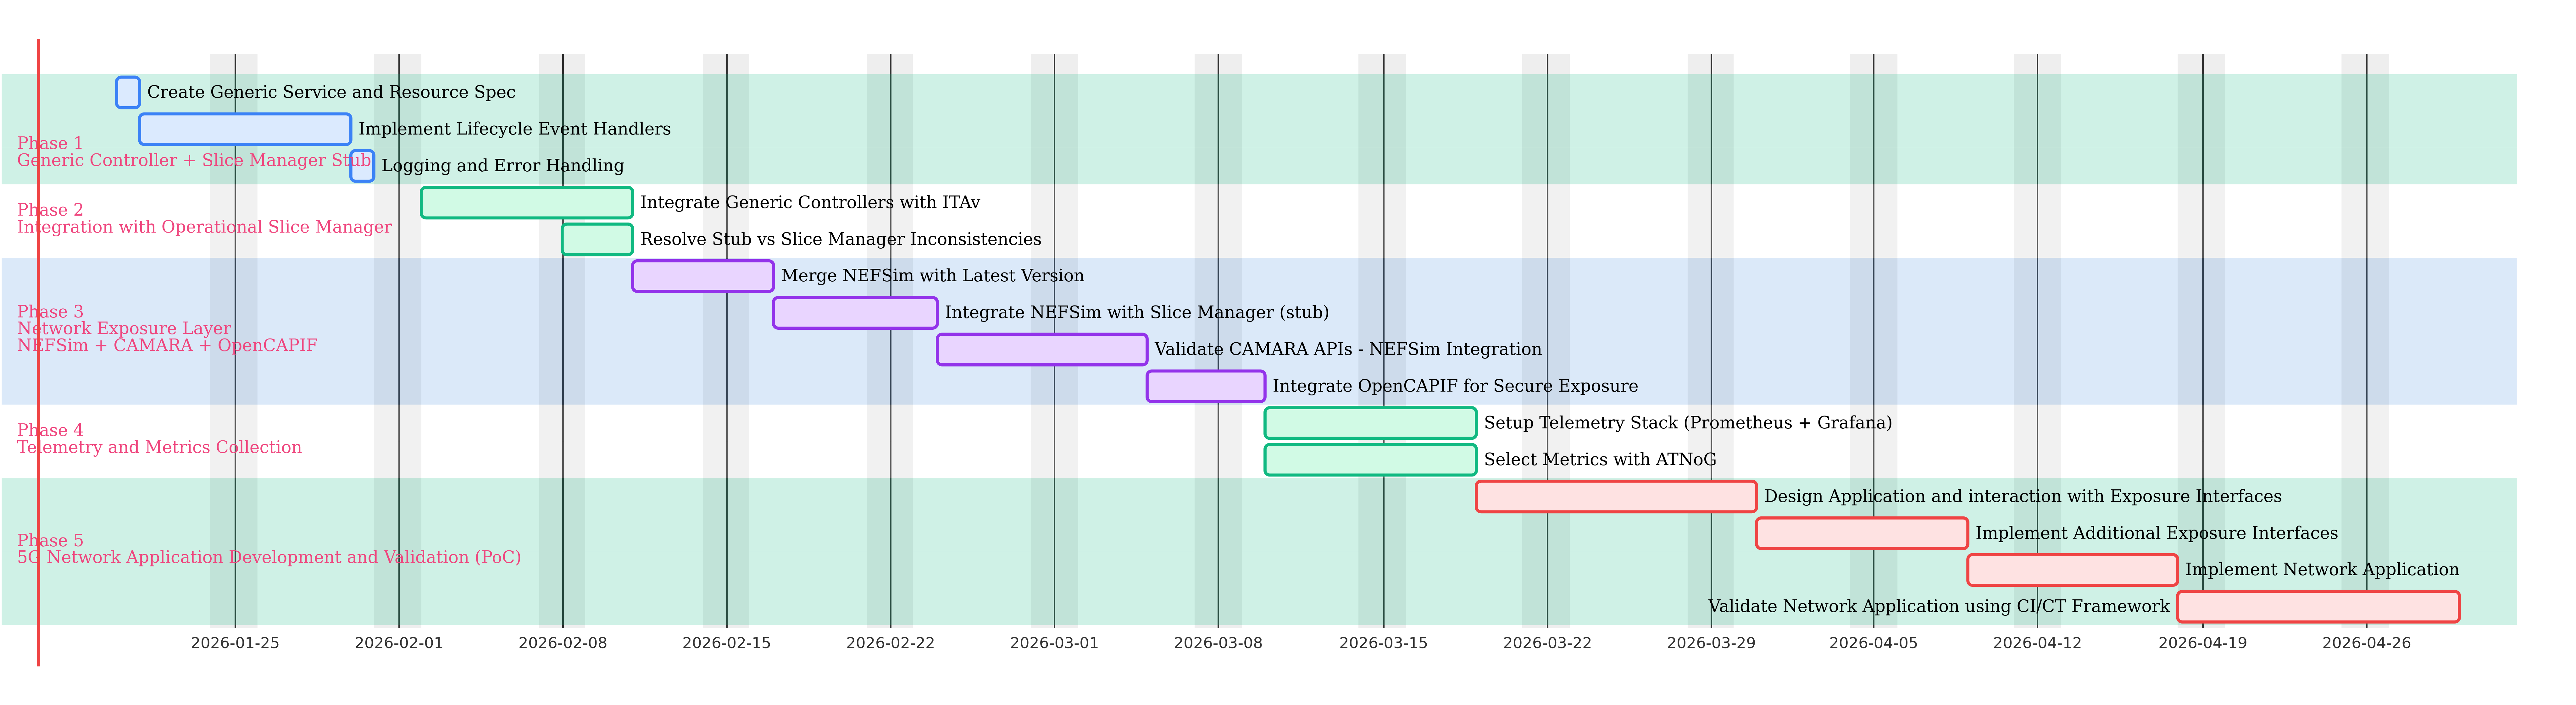
\includegraphics[width=1\linewidth]{figs/gantt_chart.png}
    \caption{Implementation Plan}
    \label{fig:ggant}
\end{figure}
\end{landscape}

The first phase of the implementation plan focuses on Generic Controllers for automated lifecycle management of network slices and \acsp{UE}. The controllers are initially integrated with a Slice Manager stub, providing a simulated interface of the provisioning capabilities of the \acs{ITAv} Slice Manager. This method is adopted to prevent any adverse impact or service disruption on the actual deployed \acs{ITAv} Slice Manager. This phase includes the design of a generic service and resource specification, including lifecycle event handlers for creation, modification, and deletion of slices and \acsp{UE}, all integrated with \acs{OSL}. Logging and error handling support should also be incorporated. As highlighted in Section \ref{chap:proposal:preliminary}, the development of the Slice Manager stub, along with the integration of the slice creation event handler have already been implemented in this first semester.


Following the initial validation with the stub, the generic controller implementations will be integrated with the operational \acs{ITAv} Slice Manager, enabling direct interaction with the 5G system infrastructure. This migration will ensure that the generic controllers can manage network slices and \acs{UE} resources in a fully operational environment. This will allow network application developers to provision and orchestrate their own network slices catered to their use case specific requirements, where they can test their network applications. This phase also includes resolving any possible inconsistencies between the stub and the the \acs{ITAv} Slice Manager, as the author didn't have access to its source code due to its proprietary nature.

Subsequently, the network exposure layer will be implemented. This phase is heavily tied to a previous \acs{ITAv} project, which integrates the following CAMARA/\acs{GSMA} Open Gateway \acsp{API} with the NEFSim~\cite{GSMANEFprojectIT}: \acs{SMS} \acs{OTP}, \acs{QoS} Profiles, Location, \acs{QoD} Provisioning, \acl{QoD}, Geofencinc Subscriptions, Device Reachability Status and Device Roaming Status. However, the given project involves the NEFSim emulating the complete network environment, thereby necessitating integration with the operational \acs{5G} system. This requires: (i) merging the project's NEFSim implementation with its latest version, (ii) integrate the NEFSim to forward all slicing related requests to the slice manager (stub), and (iii) validate the integration of the CAMARA \acsp{API} with the NEFSim, considering certain limitations encountered during this semester as well as new ones that may appear. Afterwards, the NEFSim and the CAMARA \acsp{API} must be integrated with OpenCAPIF for secure exposure. After completing this step, the testbed will enable network app developers with the necessary network interfaces, i.e. \acs{NEF} and CAMARA \acsp{API}, to interact with the network, build their applications, and orchestrate network slices and \acsp{UE}.

In the next phase, the focus is placed on monitoring and logging capabilities within the \acs{5G} network, enabling the exposure of the collected data through well-defined interfaces. To this end, Prometheus exporters are utilized for data collection, with Grafana being employed for visualization and analysis. These metrics play a critical role in the development and validation of networks applications, providing a view of the operational state and performance of the \acs{5G} network. From the metrics collected in Section \ref{sec:testingandvalidation} summarized on Table \ref{tab:metrics:all}, the following metrics of interest were selected for the validations scenarios due to their relevance in assessing operational conditions: \acs{UL}/\acs{DL} throughput, \acs{E2E} latency, \acs{CPU}, memory, \acs{RTT}, jitter, packet loss. This stage requires a deliberation phase with the \acf{ATNoG} to confirm the feasibility of collecting such  metrics.

At this step, the necessary conditions are gathered for the development of network applications, providing developers with: (i) access to the required network interfaces to interact with the network, (ii) provisioning and orchestration capabilities of \acsp{UE} and network slices tailored to their specific use case requirements, where they can deploy and actively test their applications, and (iii) the collection and exposure of network metrics to monitor and evaluate network and application performance. Therefore, a \acs{5G} Network Application will be developed as a \acs{PoC}, leveraging the implemented northbound \acsp{API} or additional \acsp{API} developed as required by the specific use case. This step encompasses the full design, implementation and validation of the network application and required exposure interfaces, ending with its provisioning as an \acs{OSL} service and evaluation via the \acs{CI}/\acs{CT} framework.



% \section{Preliminary Results}
\label{chap:proposal:preliminary}

The first semester was dedicated to establishing a robust foundation for the dissertation, conducting the State of the Art, while also performing some  preliminary work and exploratory investigations. These initial activities were essential for identifying certain limitations and establishing the groundwork for the functionalities to be implemented in the second semester. This section focuses on the preliminary activities undertaken during the first semester.

The initial phase of this preliminary work involved the deployment and integration of OpenCAPIF for securing a CAMARA \acs{QoD} \acs{API} stub, generated from its Open\acs{API} spec. This contributed to the familiarization with the CAMARA initiative and the \acs{QoD} \acs{API}, marking an important milestone in the development process with the integration of OpenCAPIF, as integrating OpenCAPIF with other \acsp{API} will follow the same approach.

The next task involved the development of the Slice Manager stub. This proved to be a particularly demanding task, as the author did not have access to the source code due to its proprietary nature, requiring the implementation of the \acs{API} solely from a limited set of example interactions (request and response). This extended the development time and  several additional meetings to clarify requirements.

Afterwards, the project referenced in Section \ref{chap:proposal:implementation}, which integrated \acs{GSMA} Open Gateway \acsp{API} and the NEFSim, was introduced with the goal of integrating its slicing functionalities with the Slice Manager stub. However, some inconsistencies regarding the integration were found, which required the author to focus on the additional task of validating and resolving these interactions. This effort is still under progress.

In paralell, it was necessary to become familiar with \acs{ITAv}'s infrastructure, specifically its \acs{OSS}: \acl{OSL}. This involded understanding the \acs{TMF}'s concepts of service and resource, deploying an instance of \acs{OSL} and exposing a Helm chart in \acs{OSL}'s Service Catalog, allowing the automated provisioning of instances upon request. Subsequently, with the goal of managing the lifecycle of slices and \acsp{UE} via the Slice Manager (currently stub), the generic controller capabilities of \acs{OSL} were explored. This culminated in the development of a Slice Generic Controller and a lifecycle management handler responsible for the creation phase of a slice by interacting with the Slice Manager, when provisioned through \acs{OSL}~\cite{OSLSlicingGcontrollerGithub}. This milestone is particularly significant, as the same approach will be applied to update and deletion operations, not only for slices but also for \acsp{UE}, which are included among the first tasks outlined in the implementation plan for the second semester in Section \ref{chap:proposal:implementation}.


This chapter addresses the work proposal for the dissertation. It proposes a testbed to establish an open, programmable environment that simplifies access to the network services offered by \acs{5G} systems, through standardized network exposure interfaces. This chapter identifies the overall design and the capabilities such an environment must provide so verticals can implement and validate their use cases. These are: (i) \acs{5G} resource lifecycle management, providing mechanisms to create, configure, and manage network slices and their associated \acsp{UE} to meet the heterogeneous requirements of each vertical (Section~\ref{chap:proposal:resource_lifecycle}); (ii) network exposure, letting verticals interact with the \acs{5G} control plane to request and configure the network according to their service requirements (Section~\ref{chap:proposal:exposure}); (iii) network observability, providing applications with relevant network data to inform decision-making and trigger appropriate actions (Section~\ref{chap:proposal:observability}); and (iv) service delivery, through which network slices and any services supporting the experiment can be ordered and managed on demand by third parties (Section~\ref{chap:proposal:delivery}). Integrating all these capabilities in a single end-to-end platform, whose architecture is defined in Section~\ref{chap:proposal:architecture}, advances the existing literature on future network testbeds, supporting interoperable service management aligned with \acs{TMF} \acs{ODA}. Section~\ref{chap:proposal:use-case} introduces a multi-vertical use case to demonstrate the interfaces and capabilities available in the testbed. Section~\ref{chap:proposal:capabilities} summarizes these capabilities, describing how the provided mechanisms support the requirements of the considered use case. Finally, Section~\ref{chap:proposal:validation} defines the validation methodology proposed to assess the resulting vertical application and, consequently, the exposed testbed capabilities.

\section{Architecture}
\label{chap:proposal:architecture}

\begin{figure}[tp]
    \centering
    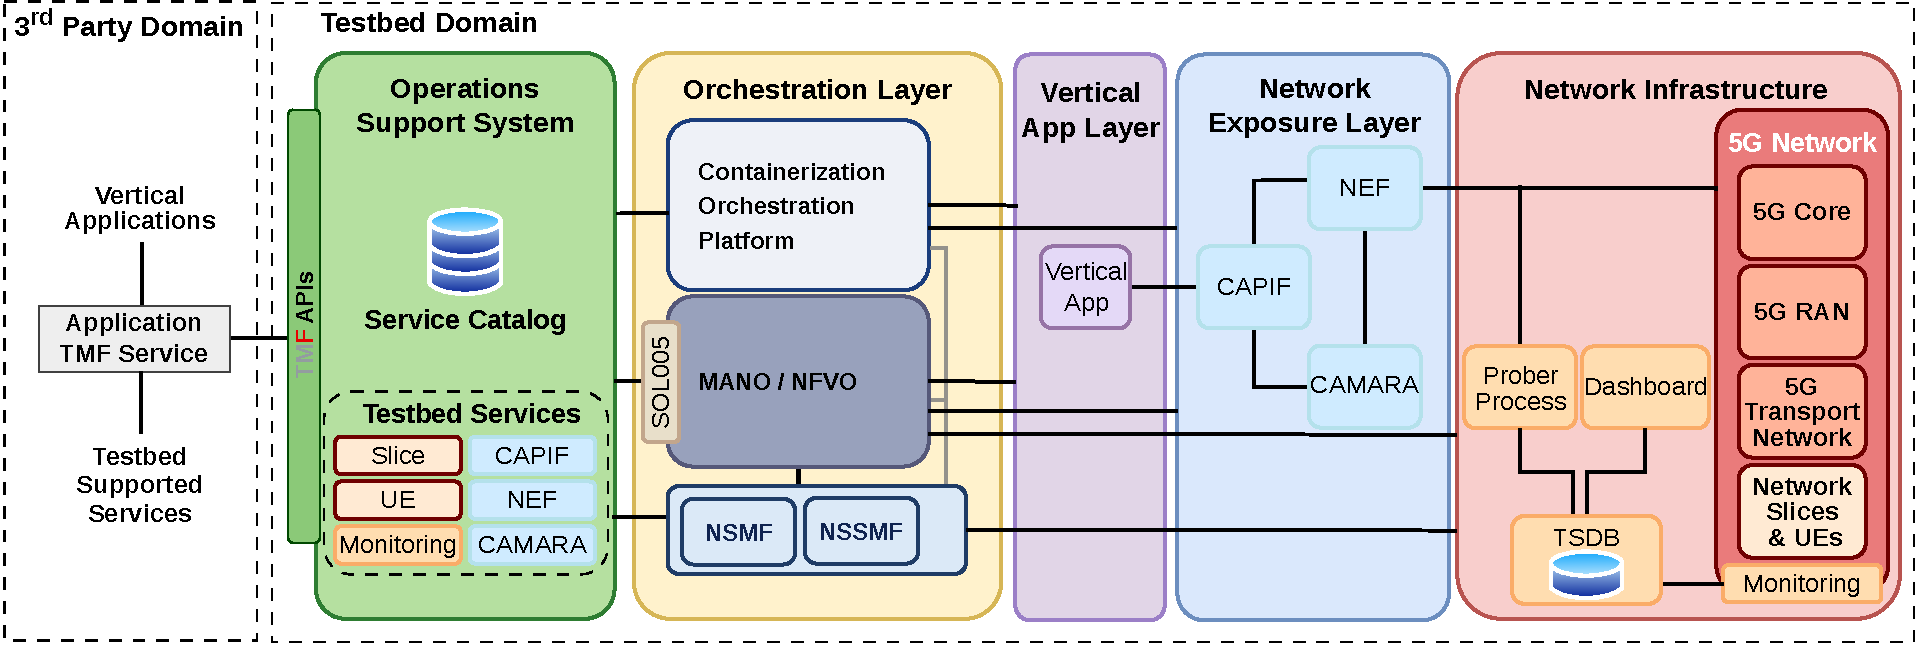
\includegraphics[width=1\linewidth]{figs/drawio/proposed_architecture.pdf}
    \caption{Proposed Testbed Architecture}
    \label{fig:proposal:architecture}
\end{figure}

According to the objectives delineated in Section \ref{chap:introduction:objectives}, the proposed testbed should offer vertical industries an experimentation environment to develop and validate network applications over a real \acs{5G} system. Figure~\ref{fig:proposal:architecture} shows the proposed architecture, separating the third-party domain, where verticals order and manage their experiments, from the testbed domain, where experiments are deployed and executed. The testbed domain follows a layered structure comprising an Operations Support System, the orchestration layer, the vertical application layer, the network exposure layer and the network infrastructure, including network monitoring.

For this purpose, third parties must be able to self-provision complete network environments tailored to their application requirements, without needing to interact with the underlying infrastructure. To this end, the \acs{OSS} should act as the main entry point to the testbed for all interactions regarding the ordering and provisioning of resources. Complete experiments comprise interdependent components, including slices, \acsp{UE}, exposure interfaces, monitoring, and vertical applications, which may rely on distinct deployment mechanisms, often through proprietary interfaces. Requiring verticals to interact with these components directly would expose internal details of the testbed, demand technology-specific knowledge, and introduce manual configuration, compromising reproducibility.

Instead, the \acs{OSS} should expose \acs{TMF} Open \acsp{API} following the \acs{TMF} \acs{ODA}, allowing verticals to discover, order, and manage services through standardized interfaces, independently of how they are realized. Centralizing experiment provisioning through the \acs{OSS} would ensure each experiment is instantiated consistently, in the order imposed by their dependencies. The services offered by the testbed should be published in a service catalog within the \acs{OSS}. Vertical applications should also be onboarded into this catalog as \acs{TMF} services, as the other testbed services. Their design and delivery workflows are detailed in Section~\ref{chap:proposal:delivery}.

Nevertheless, an \acs{OSS} is not an orchestrator and should delegate the orchestration and provisioning of resources and network applications to the orchestration layer, which would host the components responsible for the actual deployment and lifecycle management of each resource. As the testbed must accommodate both cloud-native and virtualized workloads, this layer should include a container orchestration platform and a \acs{NFVO}, integrated via the \acs{ETSI} \acs{SOL}005 interface. The former would deploy containerized components, such as the vertical applications, the exposure components and the monitoring components, while the latter would deploy \acs{NFV}-based network services.

To accommodate the diverse \acs{QoS} requirements of applications across different vertical sectors, and enable multiple experiments to coexist on a shared physical infrastructure, network slicing should be employed, establishing isolated logical networks tailored to the specific needs of each experiment. For this reason, orchestration layer must also include the \acs{NSMF} and the \acs{NSSMF}, to which the \acs{OSS} forwards the network slice requirements derived from each slice. The \acs{NSMF} manages the lifecycle of each \acs{NSI} and delegates its constituent \acsp{NSSI} to the \acs{NSSMF}, which configures the corresponding resources across the \acs{5G} network, relying on the \acs{NFVO} whenever virtualized network functions must be orchestrated.

The vertical application layer should host the network applications developed by third parties, deployed by the orchestration layer once ordered through the \acs{OSS}. Although these applications would run within the testbed domain, their only means of interacting with the \acs{5G} network should be the network exposure layer, through which they could adapt the network to their requirements and react to changes in network conditions. This leads to another key objective of this dissertation: the secure exposure of network capabilities via northbound \acsp{API}.

As highlighted in Section~\ref{sec:sba:nef}, the \acs{NEF} is the core network function of the \acs{5G} \acs{SBA} responsible for securely exposing network capabilities and events to third parties. The testbed follows this same principle, relying on the \acs{NEF} as the main gateway for \acs{5G} programmability. However, leveraging these capabilities typically requires an understanding of the underlying \acs{3GPP} procedures, which introduces a significant barrier for vertical developers who may lack the specialized telecom expertise.

To address this challenge, CAMARA services should be introduced, providing a standardized set of network \acsp{API} that act as a translation layer between the complex \acs{3GPP} \acs{NEF} and developer-friendly interfaces, at the cost of reduced control over the network. Offering both interfaces would allow each vertical to select the abstraction level that best fits its application and expertise level. As the exposure interfaces are offered to external parties, there is also a need of a common governance mechanism for the secure publication, discovery and consumption of all testbed northbound \acsp{API}, which should be fulfilled by \acs{CAPIF}.

Lastly, the network infrastructure layer should encompass the \acs{5G} system over which experiments are executed, comprising the \acs{5GC}, the \acs{RAN} and the \acs{TN}. To support adaptive application behavior, the testbed must monitor the network autonomously. This requires monitoring components to be integrated with the network infrastructure, storing the collected metrics on a \ac{TSDB}, through which they can be made available to third parties via the testbed's exposure \acsp{API}, i.e. \acs{NEF} and CAMARA. The testbed should support both passive (autonomous) and active (probing) monitoring approaches, which should both be observable by the experimenter through visual dashboards. In order to validate the testbed, a \acs{5G} network application will be onboardded and developed leveraging the envisioned northbound interfaces, catering to the specific requirements of the \acs{PPDR} and automotive vertical sectors.

\section{\acs{5G} Resource Lifecycle Management}
\label{chap:proposal:resource_lifecycle}

\begin{figure}[tp]
    \centering
    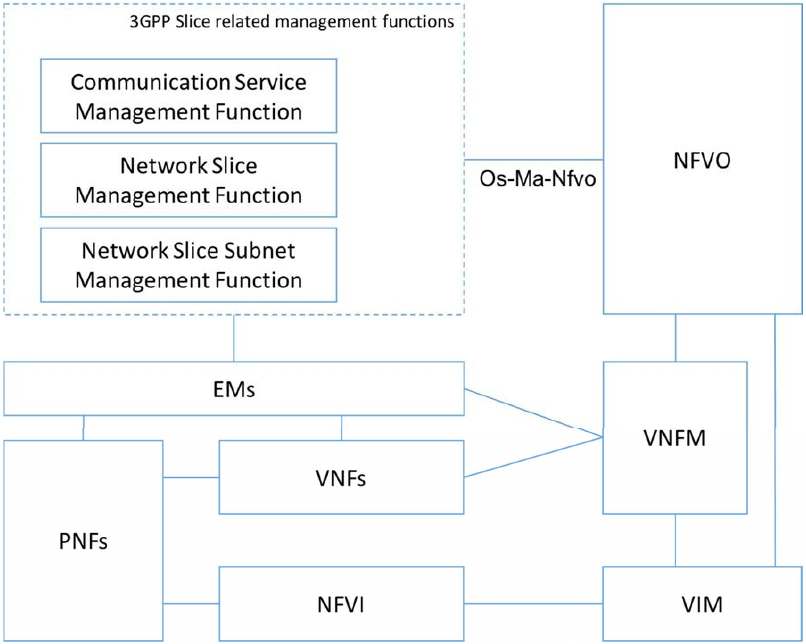
\includegraphics[width=0.7\linewidth]{figs/slicing_management_nfv.png}
    \caption{Network Slice Management in an \acs{NFV} framework~\cite{ETSI_GR_NFV_EVE_012_V3_1_1}}
    \label{fig:proposal:resource_lifecycle:slice_mgmt_nfv}
\end{figure}

The testbed must be designed to support network applications across diverse vertical sectors, each imposing distinct \acs{QoS} requirements. As introduced in Section~\ref{sota:slicing}, network slicing provides the mechanism for meeting these heterogeneous requirements by partitioning the physical infrastructure into isolated logical networks, called slices, each tailored to specific \acs{QoS} targets.

Therefore, in order to achieve this objective and cater to the use cases of a broad range of verticals, the testbed should support network slicing, covering all phases of the \acs{NSI} lifecycle: preparation, commissioning, operation, and decommissioning. Managing and orchestrating these phases correctly, demands the coordinated operation of the management functions discussed in Section~\ref{sec:slice:lifecycle}: the \acs{CSMF}, the \acs{NSMF} and the \acs{NSSMF}.

The interaction between these management functions and the \acs{NFV} framework is depicted in Figure~\ref{fig:proposal:resource_lifecycle:slice_mgmt_nfv}, as described in \acs{ETSI} GR \acs{NFV}-EVE 012~\cite{ETSI_GR_NFV_EVE_012_V3_1_1}. In this framework, the \acs{3GPP} slice related management functions would interact with \acs{NFV-MANO} through the \texttt{Os-Ma-nfvo} reference point exposed by the \acs{NFVO}~\cite{ETSI_GR_NFV_EVE_012_V3_1_1} (\acs{SOL}005 is the protocol specification that implements \texttt{Os-Ma-nfvo}). To properly interface with \acs{NFV-MANO}, the \acs{NSMF} and the \acs{NSSMF} should determine the \acsp{NS}, \acsp{VNF} and \acsp{PNF} capable of supporting the resource requirements of an \acs{NSI} or \acs{NSSI}, as well as whether existing instances can be reused or new ones must be created. For this purpose, these functions would have to maintain an association between network slice templates and \acsp{NSD}, and between \acs{NSI} identifiers and \acs{NS} instance identifiers. Consequently, from a resource management perspective, an \acs{NSI} would be mapped to one or more \acs{NS} instances, with the same principle applying to \acsp{NSSI}.

The proposed architecture presented in Figure~\ref{fig:proposal:architecture} incorporates the aforementioned management services. In this architecture, the \acs{CSMF} role is fulfilled by the \acs{OSS} system, which is responsible for exposing the communication services to customers, translating them into network slice requirements and delegating them to the \acs{NSMF}. Then, according to these requirements, the \acs{NSMF} and \acs{NSSMF} coordinate the instantiation and lifecycle management of \acsp{NSI} and their constituent \acsp{NSSI}. Additionally, both the \acs{NSMF} and the \acs{NSSMF} interact with the \acs{NFVO} whenever virtualized network functions must be orchestrated.

This mapping also defines the involvement of \acs{NFV-MANO} in each phase of the \acs{NSI} lifecycle~\cite{ETSI_GR_NFV_EVE_012_V3_1_1}, presented in Section~\ref{sec:slice:lifecycle}. During preparation, the requirements of a network slice template should be fulfilled by \acsp{NSD} previously onboarded on the \acs{NFVO}, or otherwise lead to the onboarding of a new \acs{NSD}. Commissioning would trigger the instantiation of the underlying \acsp{NS}, while the configuration of the application layer of the constituent \acsp{NF} would remain a responsibility of the \acs{NSMF} or \acs{NSSMF} and the associated element managers. During operation, \acs{NFV-MANO} would only intervene in the performance, fault and lifecycle management of virtualized resources, such as scaling an \acs{NS} to expand an \acs{NSI}. Finally, decommissioning would trigger the termination of the underlying \acs{NS} instances.

However, as highlighted in Section~\ref{sota:slicing}, network slices span the various domains of the \acs{5G} System, i.e. the \acs{RAN}, the \acs{CN} and the \acs{TN}. In practice, each of these domains may be managed by its own \acs{NSSMF}, or by multiple \acsp{NSSMF}, responsible for the \acsp{NSSI} within that domain~\cite{ETSI_TS_128_533_V19_3_0}. For instance, the \acs{RAN} \acs{NSSMF} may interface with \acs{RAN} controllers to request \acs{RAN} resources and the transport \acs{NSSMF} may interface with an \acs{SDN} orchestrator to request certain links. The \acs{NSMF} then coordinates the \acsp{NSSMF} of each domain to manage the end-to-end \acs{NSI}.

Moreover, the management functions discussed so far are not the only components involved in network slicing. While these are responsible for the provisioning and lifecycle of network slices, the \acsp{NF} of the \acs{5GC} are also aware of the provisioned slices, incorporating mechanisms to perform operations scoped to a specific slice, identified by its \acs{S-NSSAI}~\cite{ETSI_TS_123_501_V16_9_0}. Among them, the \acs{NSSF} is of particular relevance, as it selects the \acsp{NSI} serving a specific \acs{UE} and determines the allowed \acs{NSSAI}, i.e. the set of slices the \acs{UE} is permitted to use. Consequently, a \acs{UE} would only be able to receive traffic within a slice when its \acs{S-NSSAI} is included on the list of allowed \acs{NSSAI} of the \acs{UE}, and a \acs{PDU} session associated with that \acs{S-NSSAI} is established. Similarly, the \acs{NEF} may restrict the exposure of network capabilities to a specific slice, as some of its northbound \acsp{API}, such as the AsSessionWithQoS \acs{API}, allow an \acs{AF} to indicate the \acs{S-NSSAI} and \acs{DNN} targeted by a request~\cite{ETSI_TS_129_122_V18_8_0}.

Therefore, apart from network slices, the testbed should also manage the \acsp{UE} that utilize them, allowing experimenters to associate each \acs{UE} with a target slice. This association requires coordinated configuration across multiple \acsp{NF} of the \acs{5GC}~\cite{ETSI_TS_123_501_V16_9_0}. For instance, the subscription data managed by the \acs{UDM} must include the \acs{S-NSSAI} of the target slice, optionally with the permitted \acsp{DNN}. Based on this subscription, the \acs{AMF}, assisted by the \acs{NSSF}, determines the \acs{NSSAI} allowed for the \acs{UE} during registration, including the \acs{S-NSSAI} of the target slice. The \acs{UE} would then establish a \acs{PDU} session indicating the \acs{S-NSSAI} and \acs{DNN} of the target slice. Consequently, the lifecycle of a \acs{UE} would be bound to that of its slice, as a \acs{UE} cannot be associated with a slice that has not been provisioned. Decommissioning a slice may also lead the \acs{AMF} to release the \acs{PDU} sessions of its associated \acsp{UE}.

Operations for the provisioning and association of network slices and \acs{UE}, should be made available to third parties for experimentation, abstracted from the underlying infrastructure. Experimenters should only have to be exposed to, and configure, the parameters relevant to their use case, such as the \acs{QoS} requirements for the slice and the identifier of the \acs{UE}. Once again, in the proposed architecture, this role falls to the \acs{OSS}.

Finally, the requirements of an experiment may need to be changed while it is running, for instance when a network application must be evaluated under different network conditions. Therefore, during the operation phase, the testbed should allow clients to modify the \acs{QoS} requirements of a provisioned slice and of the \acs{UE} association, without requiring the decommissioning and recreation of the corresponding resources. Apart from the \acs{OSS}, the \textit{AsSessionWithQoS} \acs{API} of the \acs{NEF} may also be used to modify, at runtime, the \acs{QoS} applied to the traffic of a \acs{UE} within a given slice, which leads to the next section on network programmability.

\section{Network Exposure}
\label{chap:proposal:exposure}

As outlined in Section \ref{sec:sba:nef}, the \acf{NEF} is the main \acs{5G} core network function responsible for exposing network capabilities to external (and possibly internal) consumers. To do so, it offers a set of standardized northbound \acsp{API} that mediate access between the \acs{5G} core and consuming \acsp{AF}, while abstracting internal network functions and their implementation details. In the proposed testbed, the \acs{NEF} also serves as the primary gateway to \acs{5G} network programmability. Nonetheless, CAMARA interfaces should be provided to offer the same capabilities at an higher level of abstraction.

The coexistence of both interfaces lets each vertical choose the abstraction level that best fits its needs. While the \acs{NEF} adheres to complex \acs{3GPP} specifications but offers greater flexibility and programmability, CAMARA provides simpler, developer-facing interfaces but providing less granular control over the network. Regardless of the abstraction level, exposing these interfaces to third parties requires a common governance mechanism through which verticals can access them in a controlled and secure manner. 

The \acs{3GPP} \acs{CAPIF} fulfills such role by providing under a single platform common procedures for the secure publication, discovery and consumption of capability exposure \acsp{API}. It supports \acsp{API} specified by \acs{3GPP} or by other industry consortia, making it applicable to the northbound \acsp{API} exposed by the \acs{NEF}, as well as those defined by CAMARA.

\subsection{\acs{NEF}}
\label{chap:proposal:exposure:nef}

In the context of the proposed testbed, three \acs{NEF} northbound \acsp{API} are considered to address distinct, yet complementary aspects of network application behavior. The \textit{AsSessionWithQoS} \acs{API} targets \acs{QoS} control, providing applications with the means to establish and manage application sessions with specific \acs{QoS} profiles designed to guarantee, for example, specific bandwidth or latency requirements~\cite{ETSI_TS_129_122_V18_8_0}. This supports use cases that depend on predictable network behavior, letting applications programmatically request connectivity with specific characteristics, such as guaranteed uplink throughput or traffic priority, without human intervention. Notable examples include \acs{PPDR} applications needing temporary network resources for sporadic emergencies, and real-time video applications requiring low latency (e.g. eHealth) or support for large audiences (e.g. live broadcasting).

However, passively relying on the \acs{QoS} session established via this \acs{API} is not sufficient, as undetected violations of network requirements directly risk the correct functioning of the Network Application. Therefore, there is a clear need for a mechanism capable of actively monitoring the network and detecting any violations of the defined \acs{QoS} in real time. The \textit{AnalyticsExposure} \acs{API} addresses this problem giving developers the ability to query network analytics and subscribe to analytics notifications~\cite{ETSI_TS_129_522_V18_11_0}, allowing applications to monitor network metrics and adapt their behavior according to the observed conditions.

\acs{QoS} violations and changes in network conditions are not the only criteria that can require adaptive application behavior. According to its use case, the network application may need to be notified about specific events in the \acs{3GPP} network, completely unrelated to \acs{QoS}, such as an \acs{UE} becoming unreachable or changing location. The \textit{MonitoringEvent} \acs{API} was designed to create and manage such monitoring event subscriptions~\cite{ETSI_TS_129_122_V18_8_0}, covering events such as location reporting, loss of connectivity, \acs{UE} reachability and roaming status.

These common events can trigger different operations depending on the vertical and application scenario. For example, a \acs{TL} platform may use location updates to trigger \acs{QoS} adjustments as a teleoperated vehicle enters geofenced zones~\cite{NextGenConnectivityDynamicQoS}. In this way, monitoring events complement the \textit{AsSessionWithQoS} \acs{API} by enabling applications to adapt their requested \acs{QoS} in response to changes in \acs{UE} state.

The testbed requires all three \acsp{API} to support the envisioned network application behavior. In the remainder of this section, a closer look is taken at the \textit{AsSessionWithQoS} and \textit{AnalyticsExposure} \acsp{API}, which will be addressed in the next chapter.

\subsubsection{AsSessionWithQoS \acs{API}}
\label{chap:proposal:exposure:nef:AsSessionWithQoS}

The \textit{AsSessionWithQoS} \acs{API}, originally defined in \acs{3GPP} TS~29.122~\cite{ETSI_TS_129_122_V18_8_0}, allows applications to configure sessions indicating the desired level of \acs{QoS} for a given traffic flow. Through notifications, the \acs{API} also informs the application whether the requested \acs{QoS} can be enforced in the network.

The interaction is initiated when the \acs{AS}/\acs{AF} (e.g. a network application) submits an HTTP POST request to the \acs{NEF}, carrying an \texttt{AsSessionWithQoSSubscription} resource body~\cite{ETSI_TS_129_122_V18_8_0}. This body comprises an extensive set of parameters whose presence is governed by conditional rules, depending on the remaining payload content and on the \acs{API} features supported by the \acs{5GC}. Rather than covering all of these parameters, this section focuses on the attributes that express the desired \acs{QoS} configuration.

These include the target \acs{UE}, typically identified by its \acs{IP} or \acs{MAC} address, although groups of \acsp{UE} (\texttt{extGroupId}) or a subscription identifier such as the \ac{GPSI} may also be used when the corresponding features are supported. The traffic flow subject to \acs{QoS} treatment is then described as an \acs{IP} flow (\texttt{flowInfo}) or an Ethernet flow (\texttt{ethFlowInfo}), in accordance with the type of address provided.

The requested \acs{QoS} for that flow can be defined through the \texttt{qosReference} attribute, which references pre-defined \acs{QoS} information (e.g. \acs{QCI}/\acs{5QI} and associated parameters defined by the operator), optionally complemented by \texttt{altQoSReferences}, an ordered list of alternative references ranked by priority. Alternatively, a list of alternative service requirements (\texttt{altQosReqs}) can also be specified, each containing an individual set of \acs{QoS} parameters, namely the guaranteed bandwidth in uplink (\texttt{gbrUl}) and downlink (\texttt{gbrDl}), the packet delay budget (\texttt{pdb}) and the packet error rate (\texttt{per}). Finally, the attribute \texttt{notificationDestination} supplies the \acs{URL} at which the application will receive all notification events.

The specification further defines attributes such as usage thresholds (\texttt{usageThreshold}), \acs{QoS} signalling control (\texttt{disUeNotif}), and requirements for time sensitive communications (\texttt{tscQosReq}), which are beyond the scope of the targeted used cases. It also supports \acs{QoS} monitoring, through which the application subscribes to the \texttt{QOS\_MONITORING} event to receive measurements on the established flow. These measurements are limited to packet delay (\texttt{qosMonInfo}), data rate (\texttt{qosMonDatRate}) and congestion information (\texttt{qosMonConReq}), which are usually not covered nor utilized in the examples found throughout the literature.

Following the creation request, the \acs{NEF} maps the supplied \acs{QoS} references/parameters and coordinates with the \acs{PCF} to enforce the \acs{QoS} policy. As previously mentioned, the \texttt{notificationDestination} \acs{URI} included in the subscription body designates the callback endpoint to which the \acs{NEF} will deliver notifications. These notifications are conveyed through the \texttt{UserPlaneNotificationData} payload specifying a list of event reports for the user plane. From the possible notification event types, the testbed would rely on \texttt{SUCCESSFUL\_RESOURCES\_ALLOCATION} and \texttt{FAILED\_RESOURCES\_ALLOCATION}, which indicate whether the resources required by the requested \acs{QoS} could be allocated in the network. Other events of note for the \acs{QoS} use case include \texttt{QOS\_GUARANTEED} and \texttt{QOS\_NOT\_GUARANTEED}, which indicate whether the network is currently able to meet the \acs{QoS} targets, \texttt{QOS\_MONITORING}, which delivers the \acs{QoS} monitoring measurements, and \texttt{USAGE\_REPORT}, which provides consumption information according to the \texttt{usageThreshold} provided in the request.

\begin{figure}[htpb]
    \centering
    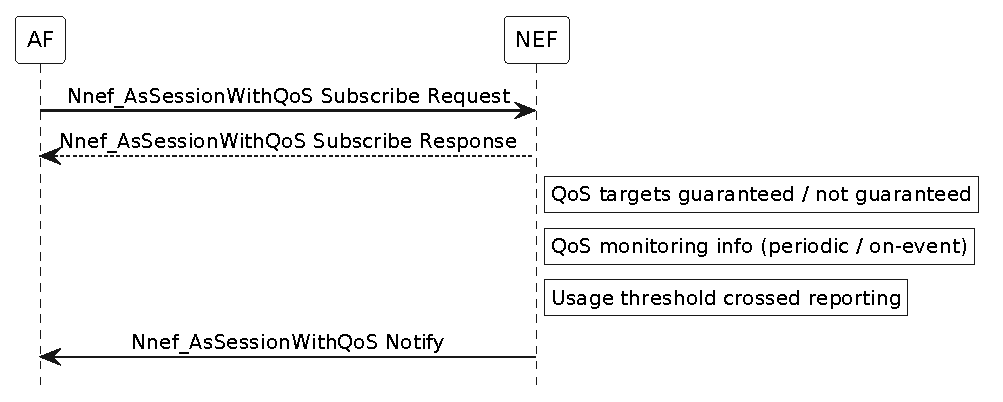
\includegraphics[width=1\linewidth]{figs/plantuml/as-session-with-qos-proposal-flow.pdf}
    \caption{Information flow for the \textit{AsSessionwithQoS} \acs{API}}
    \label{fig:flow:AsSessionWithQoSAPI}
\end{figure}

Figure \ref{fig:flow:AsSessionWithQoSAPI} highlights the described information flow for the \textit{AsSessionWithQoS} \acs{API}, obtained from the overall information flow described in TS 23.502~\cite{3GPP-23.502} and scoped to the interactions between the \acs{AF} and the \acs{NEF}, omitting internal network procedures beyond the \acs{NEF} (e.g. with the \acs{PCF}). Through this procedure, the \acs{NEF} \textit{AsSessionWithQoS} \acs{API} represents the primary programmable point in the testbed, enabling network applications to express and enforce \acs{QoS} requirements and the network conditions required to support the specific demands of each network application use case.


\subsubsection{AnalyticsExposure \acs{API}}
\label{chap:proposal:exposure:nef:AnalyticsExposure}

The \textit{AnalyticsExposure} \acs{API}, defined in \acs{3GPP} TS~29.522~\cite{ETSI_TS_129_522_V18_11_0}, allows an \acs{AF} to obtain analytics information about the network. Analytics can be retrieved through one-time fetch requests or through subscriptions, in which the \acs{NEF} notifies the \acs{AF} periodically or when specific conditions are met. Within the testbed, this \acs{API} would be the northbound interface through which the network metrics described in Section~\ref{chap:proposal:observability}, are made available to network applications.

In the \acs{5G} System, network analytics are natively produced by the \acs{NWDAF}~\cite{ETSI_TS_123_288_V18_11_0}. This function collects data scattered across multiple network functions, such as the \acs{AMF}, \acs{SMF} and \acs{UPF}, and derives new analytics from it, in the form of statistics or predictions. The \acs{NEF} then exposes these analytics to external consumers through the \textit{AnalyticsExposure} \acs{API}. However, although the specification defines the \acs{NWDAF} as the source from which the \acs{NEF} obtains analytics~\citep{ETSI_TS_123_288_V18_11_0, ETSI_TS_129_522_V18_11_0}, the \acs{AF} interacts exclusively with the \acs{NEF} and its standardized data model, making the origin of the analytics transparent to the application. The \acs{NEF} could therefore expose analytics obtained through alternative means, such as the analysis of raw \acs{IP} traffic, as long as they follow the standardized data model. This is particularly relevant for the testbed, as it would allow network application requirements and behavior to be validated without depending on an \acs{NWDAF}.

The specification defines a set of analytics events, each associated with its own analytics payload, as listed in Table~\ref{tab:proposal:exposure:nef:analytics_events}. For instance, \texttt{DN\allowbreak\_PERFORMANCE} reports the data rate, packet delay and packet loss between \acsp{UE} and an application server, while \texttt{UE\allowbreak\_COMM} characterizes the communication of \acsp{UE} with a given application, including the exchanged traffic volume.

\begin{table}[htbp]
    \centering
    \renewcommand\tabularxcolumn[1]{m{#1}}
    \begin{tabularx}{\textwidth}{|
        >{\RaggedRight\arraybackslash}m{\widthof{\texttt{NETWORK\_PERFORMANCE}}}|
        >{\RaggedRight\arraybackslash}X|}
        \hline
        \textbf{Analytics Event} & \textbf{Description} \\
        \hline
        \texttt{UE\_MOBILITY} & Location and mobility patterns of \acsp{UE}, such as tracking areas, cells or geographical coordinates where \acsp{UE} stay over time and their direction \\
        \hline
        \texttt{UE\_COMM} & Communication patterns of \acsp{UE}, such as periodicity, duration and uplink/downlink traffic volume \\
        \hline
        \texttt{ABNORMAL\allowbreak\_BEHAVIOR} & Identifies a group of \acsp{UE} or a specific \acs{UE} with abnormal behavior, e.g. being misused or hijacked \\
        \hline
        \texttt{CONGESTION} & User data congestion in a given area, or in the area where a given \acs{UE} is located \\
        \hline
        \texttt{NETWORK\allowbreak\_PERFORMANCE} & \acs{gNB} status and resource usage, communication and mobility performance, and number of \acsp{UE} in an area of interest \\
        \hline
        \texttt{QOS\allowbreak\_SUSTAINABILITY} & Statistics on past \acs{QoS} changes or likelihood of future \acs{QoS} changes in a given area \\
        \hline
        \texttt{DISPERSION} & Locations or network slices where \acsp{UE} disperse most of their data volume and session transactions, expressed as the percentage of activity generated at each location or slice\\
        \hline
        \texttt{DN\allowbreak\_PERFORMANCE} & User plane performance, namely the average and maximum traffic rate and packet delay, and average packet loss rate \\
        \hline
        \texttt{SERVICE\allowbreak\_EXPERIENCE} & Observed service experience of \acsp{UE} in an application or network slice, expressed through the average and/or variance of the observed service mean opinion score \\
        \hline
        \texttt{E2E\allowbreak\_DATA\allowbreak\_VOL\allowbreak\_TRANS\allowbreak\_TIME} & Time to complete the transmission of a specific data volume from the \acs{UE} to the \acs{AF}, or vice versa \\
        \hline
        \texttt{MOVEMENT\allowbreak\_BEHAVIOUR} & Analytics information (statistics or predictions) regarding e.g. the number, direction and velocity of \acsp{UE} during an analytics target period in a target area \\
        \hline
        \texttt{WLAN\allowbreak\_PERFORMANCE} & Quality and performance of the \acs{WLAN} connection of \acsp{UE} according to their location \\
        \hline
        \texttt{NS\allowbreak\_LOAD\allowbreak\_LEVEL} & Load level of a network slice or network slice instance \\
        \hline
        \texttt{RELATIVE\allowbreak\_PROXIMITY} & Relative proximity among a set of \acsp{UE} \\
        \hline
    \end{tabularx}
    \caption{Analytics events defined for the \textit{AnalyticsExposure} \acs{API}~\cite{ETSI_TS_123_288_V18_11_0, ETSI_TS_129_522_V18_11_0}}
    \label{tab:proposal:exposure:nef:analytics_events}
\end{table}

Figure~\ref{fig:flow:AnalyticsExposureAPI} depicts the information flow for both interaction models of the \textit{AnalyticsExposure} \acs{API}, scoped to the interactions between the \acs{AF} and the \acs{NEF}~\cite{ETSI_TS_123_288_V18_11_0, ETSI_TS_129_522_V18_11_0}. In the subscription model, the \acs{AF} specifies the analytics events of interest, optionally restricted to a set of target \acsp{UE} and to event-specific filters, together with the reporting information, such as the notification method, reporting period and maximum number of reports. The reporting information may also delimit the time period to which the analytics refer. While a past period yields statistics on observed conditions, a future period yields predictions, accompanied by a confidence level, provided that the analytics source (e.g. the \acs{NWDAF}) supports them. The request also carries the callback \acs{URI} to which the \acs{NEF} delivers the analytics notifications, according to the requested reporting information. In the fetch model, the \acs{AF} requests a single analytics event, characterized in the same way, and the analytics are returned directly in the response.

\begin{figure}[htpb]
    \centering
    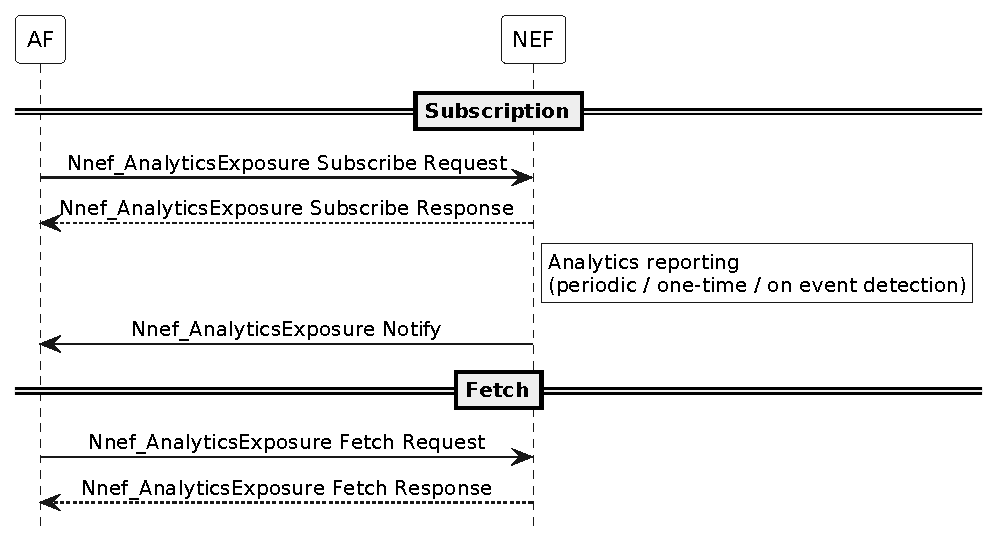
\includegraphics[width=1\linewidth]{figs/plantuml/analytics-exposure-proposal-flow.pdf}
    \caption{Information flow for the \textit{AnalyticsExposure} \acs{API}}
    \label{fig:flow:AnalyticsExposureAPI}
\end{figure}

These analytics events must be integrated with the testbed's monitoring capabilities. This way, network conditions, observed by a monitoring framework, can be exposed through the \textit{AnalyticsExposure} interface and delivered to vertical applications as they change, without the applications continuously polling the network.

In this role, the \acs{API} acts as the bridge between internal network observability and the network application layer, allowing (i) applications to adapt their behavior to the observed, and possibly future, network conditions and (ii) clients to obtain assurance that the network delivers the performance expected for their slice or \acs{QoS} session. Ultimately, the exposed analytics also support the validation of the network application's behavior against its declared requirements, discerning degraded network conditions from bad application logic.

\subsection{CAMARA \acsp{API} Integration}
\label{chap:proposal:exposure:camara}

Network application developers who wish to incorporate adaptive network behavior into their applications must interact with the network through the \acs{NEF} northbound \acsp{API} described in Section~\ref{chap:proposal:exposure:nef}. This can be accomplished in one of the following ways: (i) interacting directly with the \acs{NEF} northbound \acsp{API}, which requires familiarity with the \acs{3GPP} ecosystem, specifications and data models, imposing a significant burden on developers lacking the necessary telco expertise; or (ii) interacting with the network through CAMARA \acsp{API}, which abstract the complexity and underlying interactions with the \acs{NEF} and any other components contributing to the offered service, through a user-friendly interface.

The CAMARA initiative focuses on standardizing \acsp{API} at the northbound of the network, defining what capabilities are exposed and how application developers can interact with them to easily integrate network behavior into their applications. However, the southbound realization of those northbound \acsp{API}, i.e. their internal implementation, is deliberately left to each network operator. Nevertheless, \acs{GSMA} produces guideline documents, such as \textit{\acs{NBI} \acsp{API} Realisation in the \acs{SBI}}~\cite{gsmaNbiRealization}, describing how CAMARA \acs{API} operations can be realized through the \acsp{API} and procedures available in the operator's network, including via \acs{NEF} northbound interfaces.

The CAMARA \acsp{API} integration proposed in this section is derived from this reference realization model, mapping CAMARA operations to the corresponding \acs{NEF} interactions. Under this model, each CAMARA \acs{API} considered in the testbed has a counterpart among the \acs{NEF} northbound \acsp{API}, exposing a simplified view over the same network capability. However, not all CAMARA \acsp{API} map directly to \acs{NEF} interfaces, as some provide auxiliary functionality within the CAMARA ecosystem, such as the \textit{Application Profiles} \acs{API}. Table~\ref{tab:proposal:exposure:camara:nef_mapping} presents the \acs{NEF} and CAMARA \acsp{API} considered for the testbed, organized by the network capabilities they expose and accompanied by representative vertical use cases.

\begin{table}[htbp]
    \centering
    \renewcommand\tabularxcolumn[1]{m{#1}}
    \begin{tabularx}{\textwidth}{|
        >{\RaggedRight\arraybackslash}m{\widthof{\acs{QoS} control}}|
        >{\RaggedRight\arraybackslash}m{\widthof{\textit{AsSessionWithQoS}}}|
        >{\RaggedRight\arraybackslash}m{\widthof{Device Reachability Status,}}|
        >{\RaggedRight\arraybackslash}X|}
        \hline
        \textbf{Capability} & \textbf{\acs{NEF} \acs{API}} & \textbf{CAMARA \acs{API}} & \textbf{Use Cases} \\
        \hline
        \acs{QoS} control & \textit{AsSessionWithQoS} & \acs{QoD} & \acs{QoS} guarantees in \acs{PPDR}, eHealth,\newline live broadcasting \\
        \hline
        \acs{UE} event monitoring & \textit{MonitoringEvent} & Device Location,\newline Device Reachability Status,\newline Device Roaming Status & Geofencing,\newline fleet tracking,\newline detection of unreachable or roaming devices \\
        \hline
        Network analytics & \textit{AnalyticsExposure} & Application Profiles,\newline Connectivity Insights Subscriptions & Bitrate adaptation in video streaming,\newline detection of degraded network conditions \\
        \hline
    \end{tabularx}
    \caption{Correspondence between \acs{NEF} and CAMARA \acsp{API}}
    \label{tab:proposal:exposure:camara:nef_mapping}
\end{table}


Among these, the following subsections detail the proposed \acs{NBI} realization procedure for the \textit{Application Profiles} and \textit{Connectivity Insights Subscriptions} CAMARA \acsp{API}, which will be subject to implementation in the following chapter.

\subsubsection{Application Profiles \acs{API}}
\label{chap:proposal:exposure:camara:profiles}

The \textit{Application Profiles} \acs{API} enables network application developers to share essential information about their applications with the network and other CAMARA \acsp{API}, informing their behavior and decisions~\cite{CAMARAApplicationProfiles}. The \acs{API} focuses on defining network quality thresholds and compute resource requirements needed by the application, which naturally translate into a broad range of use cases. Across media streaming, online gaming, and video conferencing, services can benefit from the use of such an \acs{API} to verify network conditions (e.g. bandwidth, latency, jitter, packet loss) against the desired requirements and dynamically adapt their behavior accordingly. The same profile may also assist network operators in allocating resources and defining \acsp{SLA}, based on the application’s defined needs.

Figure~\ref{fig:flow:CAMARAapplicationProfiles} illustrates the \acs{NBI} realization for the \textit{Application Profiles} \acs{API}, as defined in the \acs{GSMA} reference model~\cite{gsmaNbiRealization}. Under this model, the CAMARA \acsp{API} are exposed by an Operator Platform, acting as an \acs{AF} encapsulating the \acs{NEF}, which internally defines a series of functional blocks, such as the \acs{NBI} \acs{API} Gateway, i.e. the CAMARA northbound endpoints. The Operator Platform also defines the Application Profile Storage Function, which can be considered as a stateful component (database) for storing created application profiles.

The \acs{API} exposes all the endpoints necessary to perform all \acs{CRUD} operations on an Application Profile~\cite{CAMARAApplicationProfilesRelease}. An Application Profile, expressed by the \texttt{ApplicationProfile} schema, defines application thresholds provided for network quality, including packet delay budget, minimum downstream and 
upstream rates, packet error loss rate and jitter, as well as compute resource requirements, such as target min \acs{CPU}, memory and \acs{GPU} specification.

\begin{figure}[htpb]
    \centering
    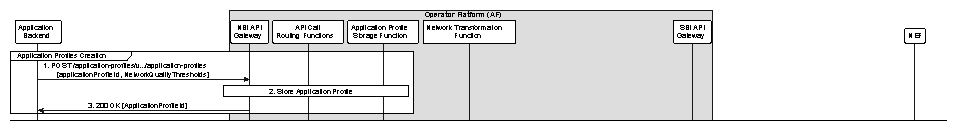
\includegraphics[width=1\linewidth]{figs/gsma-application-profiles.pdf}
    \caption{\acs{NBI} Realization for Application Profiles \acs{API}~\cite{gsmaNbiRealization}}
    \label{fig:flow:CAMARAapplicationProfiles}
\end{figure}

The sequence diagram focuses on the application profiles creation procedure. The application backend, e.g. a network application, submits a POST request to the CAMARA \acs{API} endpoint specifying the profile application requirements through the \texttt{Application\allowbreak Profile\allowbreak Request} record~\cite{CAMARAApplicationProfilesRelease}. On success, CAMARA stores the profile on the local storage repository and returns the created resource identified by a unique profile identifier. This identifier will subsequently be referenced/used in all further \acs{API} operations (retrieval, update and deletion), or by any other CAMARA \acsp{API} that consume the profile.

Throughout this workflow, there is no interaction with the \acs{NEF} or the \acs{5GC}, showcased by the absence of requests to the Network Transformation Function (i.e. the CAMARA translation layer) and the \acs{SBI} \acs{API} Gateway. This emphasizes the role of the \textit{Application Profiles} \acs{API} as a management interface over a shared profile repository, storing requirement declarations that other CAMARA \acsp{API} and network systems may reference/use to make their own decisions, as is the case of the \textit{Connectivity Insights Subscriptions} \acs{API}, discussed in the following section.

\subsubsection{Connectivity Insights Subscriptions \acs{API}}
\label{chap:proposal:exposure:camara:insights}

The \textit{Connectivity Insights Subscriptions} \acs{API} allows developers to receive continuous updates about network quality through event notifications~\cite{CAMARAConnectivityInsightsSubscriptions}. More specifically, applications can leverage this \acs{API} to monitor network conditions in real-time, receiving alerts when quality metrics fall outside the thresholds defined in their application profile, declared via the CAMARA \textit{Application Profiles} \acs{API}. Therefore, this \acs{API} represents the actual mechanism that makes the use cases specified in the previous section possible. Services which previously used profiles to declare their throughput thresholds, can now subscribe to receive notifications the moment those thresholds are breached, allowing them to take adaptive/proactive measures and prevent service disruption.

Figure~\ref{fig:flow:CAMARAconnectivityInsightsSubscriptions} illustrates the \acs{NBI} realization for the \textit{Connectivity Insights Subscriptions} \acs{API} from the \acs{GSMA} document~\cite{gsmaNbiRealization}. The procedure assumes that an application profile is previously created, as described in Section~\ref{chap:proposal:exposure:camara:profiles} (steps 1 to 3). The application then requests the creation of the analytics subscription, specifying the target device and the application server between which monitoring takes place, along with the callback endpoint (\texttt{sink}) and the referenced application profile. The application profile thus defines the network requirements to be monitored. This establishes a direct dependency between the \textit{Connectivity Insights Subscriptions} \acs{API} and the \textit{Application Profiles} \acs{API}, as a subscription requires a previously created application profile to define the criteria against which observed network conditions are evaluated.

\begin{figure}[htpb]
    \centering
    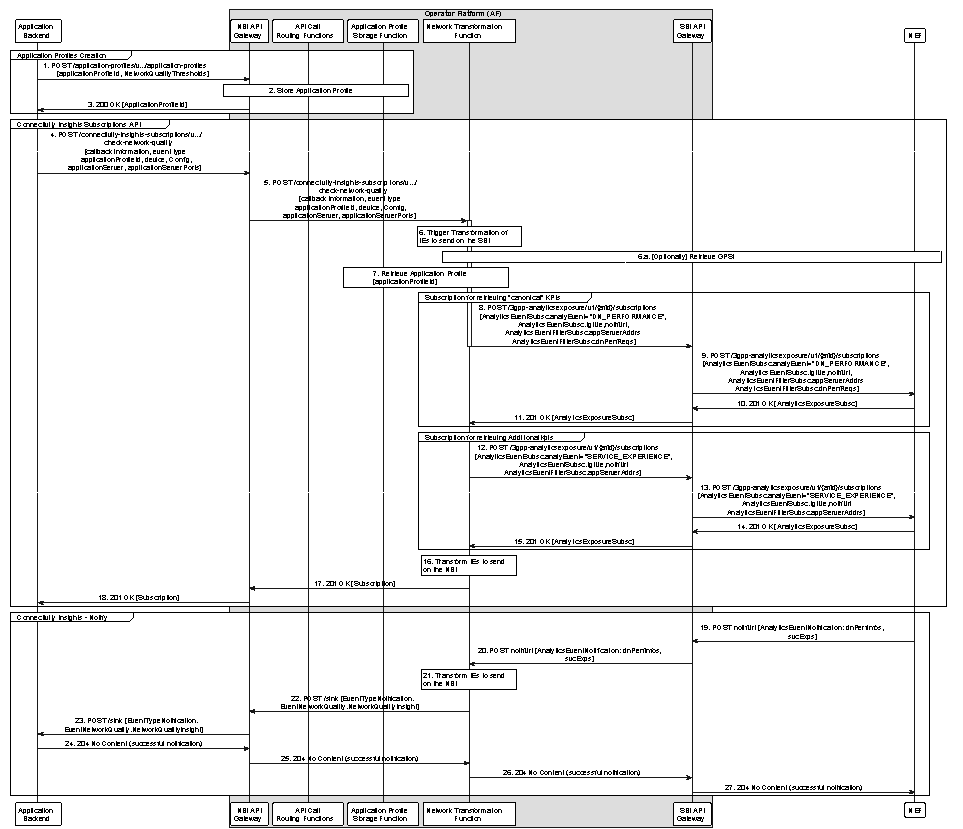
\includegraphics[width=1\linewidth]{figs/gsma-connectivity-insights-subscriptions.pdf}
    \caption{\acs{NBI} Realization for Connectivity Insights Subscriptions \acs{API}~\cite{gsmaNbiRealization}}
    \label{fig:flow:CAMARAconnectivityInsightsSubscriptions}
\end{figure}

Unlike the \textit{Application Profiles} \acs{API}, which involves no interaction with the \acs{NEF} and, consequently, no translation between the CAMARA data models and the underlying \acs{NEF} \acs{3GPP} procedures, the \textit{Connectivity Insights Subscriptions} \acs{API} encapsulates the \acs{NEF} \textit{AnalyticsExposure}~\acs{API}. After receiving the request, the CAMARA layer fetches the application profile from the datastore. The request and the retrieved profile (step 7) are then translated into one or multiple \textit{AnalyticsExposure} subscriptions, which are sent to the \acs{NEF}. The fields of the request are converted into the subscription, passing the device as the target \acs{UE} (\texttt{tgtUe}) and the addressed application server. When the device is identified by its \acs{IP} address, its \acs{GPSI} may first be retrieved from the network (step 6.a). The notification destination of each subscription (\texttt{notifUri}) is also set to the \acs{URI} of the CAMARA service, so that \acs{NEF} notifications are received by the translation layer, before being forwarded to the client. In addition, the network quality thresholds of the application profile are mapped into the reporting thresholds of the \texttt{dnPerfReqs} attribute (for the \texttt{DN\_PERFORMANCE} event), so that the \acs{NEF} notifies the Operator Platform whenever the observed performance crosses them. The reporting requirements of the subscription are, in turn, mapped into the \texttt{analyRepInfo} attribute.

The \acs{NEF} \textit{AnalyticsExposure} \acs{API} supports a wide range of analytics events, covering aspects such as network performance, \acs{UE} communication patterns and service experience~\cite{ETSI_TS_129_522_V18_11_0}. Among these, the \acs{GSMA} reference document selects two events to fulfill the analytics requirements of the \textit{Connectivity Insights Subscriptions} \acs{API}. The \texttt{DN\allowbreak\_PERFORMANCE} event is recommended to retrieve the canonical \acsp{KPI} of the application profile, i.e. the packet delay budget, the downstream and upstream rates, the packet error loss rate and the jitter. A complementary subscription for the \texttt{SERVICE\allowbreak\_EXPERIENCE} event may additionally be created to retrieve additional \acsp{KPI}, namely an indication of the radio conditions and access technology of the device, without any threshold attached.

Once the \textit{AnalyticsExposure} subscriptions are created, the reference to the CAMARA subscription is returned to the application backend. From this point forward, the communication between the involved entities, i.e. application, CAMARA and \acs{NEF}, is entirely based on callbacks. When the notification criteria are met, the \acs{NEF} sends a notification to the \texttt{notifUri} carrying the reported analytics. The CAMARA service then processes these analytics into a network quality insight, indicating, for each threshold of the application profile, if the network meets or is unable the application requirements. At the end, a second callback delivers this insight to the original \texttt{sink} specified by the application in the CAMARA subscription request.

Combined, the \textit{Application Profiles} and \textit{Connectivity Insights Subscriptions} \acsp{API} would allow a network application to declare its network requirements once and be notified whenever the network fails to meet them. The selection of analytics events, the translation into \acs{3GPP} data models and the evaluation of the reported metrics would  be completely abstracted from the consumer, allowing developers without telco expertise to incorporate network analytics into their applications.

\subsection{Secure \acs{API} Exposure via \acs{CAPIF}}
\label{chap:proposal:exposure:capif}

The \acs{NEF} and CAMARA components described in the preceding sections provide the mechanisms necessary to expose network capabilities to third parties. Together, they provide developers with the interfaces required to interact with the underlying \acs{5G} infrastructure, leveraging it to build network applications. Nevertheless, a standardized mechanism for the secure discovery, exposure, and consumption of these northbound \acsp{API} is yet to be defined.

As introduced at the beginning of this section, these northbound \acsp{API} should be exposed through a common governance mechanism, i.e. \acs{CAPIF}~\cite{ETSI_CAPIF_TS_123_222_V18_4_0}. It introduces a set of roles, namely the \acs{API} Provider, \acs{API} Invoker and \acf{CCF}, along with the procedures for \acs{API} publishing, discovery, and access control. Given its generic design, several works in the research community have treated \acs{CAPIF} as a general-purpose \acs{API} gateway with authentication and authorization capabilities, leveraging it to protect both \acs{NEF} and CAMARA northbound \acsp{API}~\citep{PathwayNaaSCAMARA,pushingBoundariesScalable5GCN}.

This dissertation follows the same interpretation, using \acs{CAPIF} as a unified secure exposure layer that consolidates common supporting capabilities into a single component, for all northbound \acsp{API} in the testbed. Under this model, (i) \acs{CCF} acts as the central control entity of the framework; (ii) both the \acs{NEF} and CAMARA \acsp{API} act as \acs{API} providers exposing interfaces to be consumed by network applications, which operate as external \acs{API} invokers; and (iii) each CAMARA \acs{API} additionally assumes the role of an internal \acs{API} invoker, interacting with \acs{NEF}'s \acs{API} to deliver its services from inside the network's trust domain.

{\spaceskip=\fontdimen2\font plus 0.5em minus \fontdimen4\font
The procedures defined in the \acs{CAPIF} architecture are realized as a collection of RESTful \acsp{API} in \acs{3GPP} TS 29.222~\cite{ETSI_CAPIF_TS_129_222_V18_6_0}, namely the \texttt{Discover\allowbreak\_Service}, \texttt{Publish\allowbreak\_Service}, \texttt{Events}, \texttt{API\allowbreak\_Invoker\allowbreak\_Management}, \texttt{Security}, \texttt{Monitoring}, \texttt{Logging\allowbreak\_API\allowbreak\_Invocation}, \texttt{Auditing}, \texttt{Access\allowbreak\_Control\allowbreak\_Policy}, \texttt{API\allowbreak\_Provider\allowbreak\_Management}, and \texttt{Routing\allowbreak\_Info} \acsp{API}.}
In the testbed, the exposure of each northbound \acs{API} would follow these procedures. Before any \acs{API} becomes available, each provider should register with the \acs{CCF} and publish its service \acs{API} information through the \acs{CAPIFAPF}. Each network application would then onboard with the \acs{CCF} to obtain its security credentials, and use the discovery interface of the \acs{CCF} to identify the exposed \acsp{API}, their endpoints, and the authorization policies governing their use. Each invocation would subsequently reach the \acs{CAPIFAEF}, which authenticates the invoker, validates the authorization issued by the \acs{CCF}, and logs the invocation for auditing. Through these onboarding and authorization policies, the set of \acsp{API} available to each network application can also be restricted~\cite{ETSI_CAPIF_TS_123_222_V18_4_0}.

As a result, rather than requiring separate onboarding, discovery, and authentication procedures for each \acs{API} suite, a single \acs{CAPIF} integration point consolidates these concerns regardless of whether the underlying \acs{API} is a \acs{3GPP} \acs{NEF} interface or a CAMARA abstraction. This significantly reduces integration complexity and aligns with the testbed's objective of providing a developer-friendly environment for the rapid development and validation of network applications.


\section{Network Observability}
\label{chap:proposal:observability}

The correct functioning of a vertical application is directly affected by the network conditions under which it operates. Undetected QoS violations or changes in network conditions may compromise or mandate different application behavior. The \textit{AsSessionWithQoS} and \textit{AnalyticsExposure} \acsp{API}, presented in the previous section, address part of this need by exposing \acs{QoS} and network analytics to external applications through their standardized interfaces. Nevertheless, these \acsp{API} provided by the \acs{NEF} constitute only the northbound interface and do not autonomously generate the underlying measurements conveyed in its payloads. These must be collected from the network and relevant network functions, such as the \acs{UPF}, \acs{SMF} and \acs{AMF}, and made available through a dedicated observation layer. In the \acs{5G} System, this role is largely assigned to the \acs{NWDAF}, which collects data from these \acsp{NF} and the management system to derive the analytics later exposed through the \acs{NEF}~\cite{ETSI_TS_123_288_V18_11_0}.

Moreover, due to the incompleteness of current \acs{NEF} (and \acs{NWDAF}) implementations, it may be necessary to implement the corresponding southbound functionality to retrieve these measurements from the testbed's monitoring mechanisms and, consequently, expose them to network applications. Without it, network applications would be unable to detect degradations of \acs{QoS} and changes or anomalies within the network through the \acs{NEF}.

In respect to this, the testbed should provide objective communication metrics that characterize network conditions as experienced by the application. For example, throughput and traffic volume measurements, relevant for assessing whether the network can sustain an application's current data rate and capacity requirements, as in smart manufacturing, where large numbers of deployed sensors continuously generate data the network must support.

In Section \ref{sec:testingandvalidation:metrics}, Table \ref{tab:metrics:all} presented the full set of metrics and \acsp{KPI} collected across the researched State of the Art. From this broader survey, the metrics most relevant to the proposed testbed have been selected and presented in Table \ref{tab:proposal:observability:metrics}, grouped by their source and identified relevance for their collection.

\begin{table}[htbp]
    \centering
    \renewcommand\tabularxcolumn[1]{m{#1}}
    \begin{tabularx}{\textwidth}{|
        >{\RaggedRight\arraybackslash}m{\widthof{NG-RAN}}|
        >{\RaggedRight\arraybackslash}m{\widthof{UL/DL throughput}}|
        >{\RaggedRight\arraybackslash}X|}
        \hline
        \textbf{Source} & \textbf{Metric} & \textbf{Relevance} \\
        \hline
        \acs{AMF} & \acs{UE} registration \& reachability state & Exposed to applications via \acs{NEF} \textit{MonitoringEvent} \acs{API}; allows adaptive application behavior on connectivity changes \\
        \hline
        \acs{SMF} & Active \acs{PDU} session count & Reflects session load at the \acs{SMF}/\acs{UPF}; supports correlation between session lifecycle events and observed metrics \\
        \hline
        \acs{UPF} & \acs{UL}/\acs{DL} throughput (per \acs{PDU} session) & Primary indicator of bitrate \acs{QoS} compliance; reflects if the \acs{QoS} profiles enforced per slice and \acs{UE} are met \\
        \hline
        \acs{UPF}, \acs{NG-RAN} & Packet loss rate & Captures data plane reliability; \newline relevant for reliability-critical applications \\
        \hline
        \acs{UPF}, \acs{NG-RAN} & \acs{UL}/\acs{DL}/round-trip packet delay & Measures delivery delay between the \acs{UE} and \acs{UPF}; essential for applications with strict latency \acs{SLA} \\
        \hline
        \acs{UPF}, \acs{NG-RAN} & Jitter & Derived from consecutive packet delay samples; critical for real-time media and control applications \\
        \hline
    \end{tabularx}
    \caption{Selected network observability metrics organized by source}
    \label{tab:proposal:observability:metrics}
\end{table}

Most metrics in Table \ref{tab:proposal:observability:metrics} would be retrieved directly from the \acs{NF} identified as their source. The exceptions are delay, packet loss and jitter, as these characterize the data path between the \acs{UE} and the \acs{UPF}, spanning both the radio and core segments of the network. Thus, delay measurements at the \acs{UPF} would rely on the \acs{QoS} monitoring procedure of the \acs{5G} System, in which the \acs{NG-RAN} reports the radio segment of the measurement, between the \acs{UE} and the \acs{NG-RAN}, and the \acs{UPF} reports the core segment, between the \acs{NG-RAN} and the \acs{UPF}~\cite{ETSI_TS_123_501_V16_9_0}. Jitter, in turn, is not directly measured, being derived by the \acs{PCF} from these delay measurements~\cite{ETSI_TS_123_501_V16_9_0}. Packet loss is likewise not covered by this procedure, being instead obtained from performance measurements collected at the \acs{NG-RAN} and at the N3 interface of the \acs{UPF}, which the \acs{NWDAF} combines into an end-to-end packet loss rate between the \acs{UE} and the \acs{UPF}~\cite{ETSI_TS_123_288_V18_11_0}.

As highlighted in Section~\ref{sec:testingandvalidation}, many validation pipelines rely on manually triggered scripts (e.g. ping, hperf) or ad hoc procedures to collect network metrics. Such an approach may be acceptable in isolated research efforts where the purpose of metrics collection is tightly scoped to a single specific goal, but is inadequate for application-level validation in the context of a testbed. For the proposed testbed, delegating this responsibility to each application (and each client) individually would not only introduce redundant and inconsistent workflows, but would also be architecturally inappropriate, as network applications will operate outside the \acs{5G} core and network application developers, being by definition external parties to the testbed, lack both the access, the insight and the expertise into the infrastructure and network internals needed to collect these measurements themselves. Not to mention that it would be a security concern.

The testbed should therefore autonomously monitor the network, without human intervention, and make the resulting metrics available to its clients, scoped to each experiment. These comprise \acs{QoS} measurements for network components, such as network slices and \acsp{UE}, as well as the workload performance of \acsp{NF}. At the application level, the testbed should also provide logs and resource metrics (e.g.~\acs{CPU} usage, memory consumption), typically sourced from orchestration platforms hosting the application and the testbed's services (e.g. Kubernetes, \acs{OSM}).

Together, these would allow network application developers to obtain insights on the network and continuously evaluate it against the declared \acs{QoS} requirements of each deployed application. It would also enable them to adjust to changing conditions and attribute observed application behavior to their implementation rather than to unknown causes. This is particularly critical in multi-tenant scenarios, where multiple applications and slices must be monitored independently and simultaneously, and can be achieved in the two following ways: passive and active monitoring.

\subsection{Passive Monitoring}
\label{chap:proposal:observability:passivemonitoring}

Passive monitoring derives network metrics by capturing and inspecting traffic at strategic observation points within the \acs{5G} core, without injecting additional load into the network. In practice, this is realized through metric exporters that expose internal telemetry data that is collected at: (i) the \acs{NF} level and (ii) other key points of the network. This approach allows to collect, from the observed traffic, metrics such as \acs{UL} and \acs{DL} throughput, packet counts and transmission error rates.

The main advantage of passive monitoring is in its non-intrusive nature. As it operates on traffic already traversing the network, it does not consume additional bandwidth, limiting itself to observing the already existing traffic. However, it is contingent on the existence of active traffic and unlike active probing techniques, cannot directly measure the network conditions as experienced by the subscriber, meaning it is not suitable, for instance, to validate end-to-end performance throughout the entire lifetime of a network slice and its \acsp{UE}.

\subsection{Active Monitoring}
\label{chap:proposal:observability:activemonitoring}

Active monitoring complements this limitation by generating synthetic network traffic between designated points (e.g. a prober and an \acs{UE}) to assess \acs{QoS} parameters on demand, independently of current application traffic. This makes it possible to directly measure metrics such as latency, \acs{RTT} and jitter, particularly relevant for domains with stringent connectivity requirements. For instance, in autonomous transportation, where latency measurements allow developers to evaluate whether communication delays are low enough for real-time vehicle control and coordination. Similarly, high packet loss directly impacts communication reliability, making it another important metric to monitor.

Active probing directly captures these metrics from the end-user's perspective, i.e. the prober, making it suitable to validate the enunciated performance of a network slice, throughout its entire lifecycle. To achieve this goal in the testbed, active monitoring must be initiated automatically upon \acs{UE} and slice provisioning, rather than issued as a one-off manual request. This requires integration between the probing mechanism and the provisioning workflow, such that probing processes are configured, instantiated, and terminated in alignment with the lifecycle of each network slice and its associated \acsp{UE}, as follows:

\begin{itemize}
    \item \textbf{Network Slice Lifecycle:} When a network slice is provisioned, a probe server is configured and deployed within, or reachable from, that slice's data plane, ready to generate and send synthetic traffic towards probing targets. Each slice should be assigned its own individual prober, allowing measurements to be collected separately for each slice and use case. Upon deprovisioning, all probing infrastructure associated with it must be cleaned up.
    \item \textbf{UE Lifecycle:} After a \acs{UE} is provisioned and attached to the slice, its \acs{IP} or \acs{MAC} address may optionally be registered as a probing target and a measurement session initiated. When the \acs{UE} is deprovisioned, the corresponding session should be terminated and the target entry removed.
\end{itemize}

However, unlike the passive alternative, active probing is inherently disruptive, as the generated traffic consumes network resources and competes with regular application traffic. For this reason, experimenters must be able to activate and deactivate active probing mechanisms on demand. This prevents synthetic traffic from negatively affecting the subscriber’s \acs{QoS}/\acs{QoE} when undesirable, while also allowing experimenters to intentionally introduce additional traffic when they need to induce adverse network conditions, such as during load testing scenarios.

Combined, passive and active monitoring form the observation layer of the proposed testbed. The collected measurements should then be delivered through programmatic interfaces, allowing vertical applications to adapt their behavior based on current network conditions. Both \acs{NEF} and CAMARA defined standardized \acsp{API} for this use case, i.e. the \textit{AnalyticsExposure} and \textit{Connectivity Insights Subscriptions} \acsp{API}, respectively. In parallel, these measurements can also be exposed through visual dashboards, for simplified metric interpretation.

\subsection{Closed-loop Optimization}

The continuous collection of network metrics through both approaches establishes the foundation for closed-loop network optimization. By feeding the collected metrics into a control component, corrective measures can be taken by the network to automatically adjust to degraded network conditions. Such actions may include adjusting the active \acs{QoS} profile via the \textit{AsSessionWithQoS} \acs{API} and/or notifying the affected network application to adapt its behavior to the new fulfilled \acs{QoS}.

In addition to such reactive measures, the collected metrics can further serve as input to the \acs{NWDAF}, as described in Section \ref{chap:proposal:exposure:nef:AnalyticsExposure}. By continuously analyzing historical and real-time network telemetry, the \acs{NWDAF} can predict degraded conditions before they actually happen. These predictions can then be consumed by the \acs{PCF}, which proactively enforces updated \acs{QoS} policies without waiting for congestion to occur. This shifts the closed-loop optimization strategy from purely corrective to a more proactive dimension, reducing the frequency and severity of service disruptions.

\section{Service Delivery}
\label{chap:proposal:delivery}

To implement and validate network applications, third parties require a network environment that reproduces the conditions under which each application is supposed to operate. The role of a testbed is not only to provide such a substrate, i.e. the actual physical network and compute infrastructure, but also to provide the necessary capabilities to configure it for each experiment, according to the requirements of the application and target vertical industry. This requires partitioning the shared infrastructure into isolated logical networks through network slicing, exposed as third-party services that let verticals configure slices tailored to their applications. Moreover, the complete lifecycle of the provisioned slices and their UE should follow widely adopted, accessible data models.

Composing complete experiments, however, requires access to other functionalities. The exposure APIs, monitoring services, and the vertical application itself must all be configured, packaged and deployed for each experiment. These capabilities should be offered as services through a single management and automation platform, traditionally an OSS. Through it, verticals can design, order, and manage services as needed, without manually interacting with the underlying infrastructure components which realize their orchestration. Centralizing the provisioning of experiments in a single platform would also ensure that each experiment is instantiated consistently, so that its results can be reproduced and compared across executions.

With this in mind, vertical clients should be able to access this platform both through a graphical interface and programmatically, via standardized APIs that support automation and integration with external tools. TMF ODA addresses this by defining TMF Open APIs to simplify service design, orchestration, and management, abstracting proprietary management interfaces so network capabilities are offered through standardized, interoperable ones.

The remainder of this section details how such a platform may support the complete lifecycle of an experiment by translating vertical requirements into services that can be provisioned and tested on the testbed.


\subsection{Service Design}
\label{chap:proposal:delivery:design}

Each functionality offered by the testbed should be described by a reusable service specification that defines the service's attributes, relationships, and constraints~\cite{SIDTMF, SID-MODELS-v250-TMF}. Following the \acs{TMF} \acs{SID} model, the proposed design distinguishes between specifications for \acsp{CFS}, which describe the service as perceived by the vertical, and \acsp{RFS}, which describe how it is realized over the underlying resources. Each \acs{CFS} exposes a set of configurable characteristics, so that verticals can parameterize services according to their application without knowledge of how these are realized within the testbed. The resulting specifications must be published in a service catalog, from which verticals can browse and order the available services through \acs{TMF} Open \acsp{API}. The \acs{OSS} should additionally provide a \acs{GUI} that allows verticals to perform these operations without directly interacting with the \acsp{API}.

Service specifications may also reference other specifications, forming composite services. A complete experiment typically requires multiple interdependent services that must be configured and provisioned together, e.g. a network slice and its attached \acs{UE}, or a network application and the \acs{5G} exposure \acsp{API} it consumes. These dependencies should be captured as a bundle of services and offered at different levels of granularity depending on the use case. For example, a network slice and its \acsp{UE} can be offered both as standalone services, to extend an existing experiment, and as a single composite service, to provision a complete environment through a single order. In either case, the system is responsible for maintaining a consistent view of the provisioned resources and their dependencies, ensuring that the relationships between them remain explicitly represented regardless of whether these are provisioned through separate service orders or at different times, e.g. when a \acs{UE} is provisioned as a standalone service and attached to a previously provisioned slice, the resulting relationship shall be registered by the system. 

To support the composition of complete experiments, the service catalog should offer the following suite of services.


\bulletparagraph{\textit{Network Slice}}

The Network Slice service should provision an \acs{NSI} tailored to the vertical's \acs{QoS} requirements, managed as established in Section~\ref{chap:proposal:resource_lifecycle}. Its characteristics should express these requirements through configurable standardized slice attributes.

In particular, the Network slice specification should be derived from the \acs{GSMA} \acs{GST}. As discussed in Section~\ref{sec:slice:lifecycle}, the \acs{GST} defines a common set of attributes to describe a network slice, such as throughput, latency, \acs{UE} density and isolation level, which are assigned concrete values in a \acs{NEST} for a specific use case~\cite{GSMA_GST}. Mapping these attributes to the characteristics of the slice service specification would allow verticals to express their requirements through a standardized vocabulary. The management plane should then translate these characteristics into concrete slice requirements that are delegated to the corresponding network slice management functions, i.e. the \acs{NSMF} and the \acs{NSSMF}, as outlined in Section~\ref{chap:proposal:resource_lifecycle}.


\bulletparagraph{\textit{User Equipment}}

The User Equipment service should transparently register a \acs{UE} with the \acs{5G} network and attach it to a provisioned network slice. The design and management of \acs{5G} \acs{UE} are defined across several \acs{3GPP} specifications, namely 3GPP TS 23.501~\cite{}, 3GPP TS 24.527~\cite{} and 3GPP TS 23.503~\cite{}. However, in contrast to network slices, no common template is standardized or recommended for the definition of a \acs{UE}. Because of this, this dissertation proposes a minimal blueprint for modeling \acs{5G} \acsp{UE}, which is presented in Table~\ref{tab:proposal:delivery:ue-blueprint}.

The blueprint identifies the requested slice for the \acs{UE} via the \acs{SST} and optional \acs{SD} fields. In addition, it specifies the aggregate bitrate limits, as well as optional static addressing for the established \acs{PDU} session. These fields constitute a minimal common set and may be extended with implementation specific parameters required by different \acs{5G} distributions.

\begin{table}[htbp]
    \centering
    \renewcommand\tabularxcolumn[1]{m{#1}}
    \begin{tabularx}{\textwidth}{|
        >{\RaggedRight\arraybackslash}m{\widthof{SessionAmbr : Downlink}}|
        >{\RaggedRight\arraybackslash}X|}
        \hline
        \textbf{\acs{UE} Parameter} & \textbf{Description} \\
        \hline
        Requested\acs{NSSAI} : \acs{SST}  & Slice Service Type that identifies the category of the network slice requested by the \acs{UE} \\
        \hline
        Requested\acs{NSSAI} : \acs{SD}  & Optional Slice Differentiator that, with \acs{SST}, forms the \acs{S-NSSAI} uniquely identifying the slice requested by the \acs{UE} \\
        \hline
        SessionAmbr : Uplink & Maximum bitrate allowed for \acs{UE} uplink traffic \\
        \hline
        SessionAmbr : Downlink & Maximum bitrate allowed for \acs{UE} downlink traffic \\
        \hline
        PduSession : IPv4 & Optional field to request a static IPv4 address for the \acs{UE} \\
        \hline
        PduSession : IPv6 & Optional field to request a static IPv6 address for the \acs{UE} \\
        \hline
    \end{tabularx}
    \caption{\acs{UE} blueprint specification}
    \label{tab:proposal:delivery:ue-blueprint}
\end{table}

As the \acs{UE} is only meaningful for the experiment in the context of a slice, the service should declare an explicit dependency to the Network Slice service. That dependency ensures the slice is active before the \acs{UE} is registered, and that the \acs{UE}’s subscription is removed from the \acs{5G} network when the slice is decommissioned.


\bulletparagraph{\textit{Network Exposure}}

The Network Exposure service should allow experimenters to setup the network exposure interfaces mentioned throughout this document, i.e. the \acs{NEF} and CAMARA \acsp{API}, published and secured through the \acs{CAPIF} framework, as described in Section~\ref{chap:proposal:exposure}. 

These interfaces cannot be deployed independently, in paralell, as they follow a strict dependency chain. \acs{CAPIF} must be available first, as the \acs{NEF} relies on it to publish and secure its \acsp{API}. The CAMARA \acsp{API}, in turn, rely on the \acs{NEF} to process their requests and are exposed through \acs{CAPIF}. Nonetheless, not every experiment requires the full exposure layer constituted by all three components. Thus, such an exposure service should support a configuration without the CAMARA \acsp{API}, for cases where the network application interacts with the \acs{NEF} directly, or relying on an alternative authentication method that does not depend on \acs{CAPIF}, preventing it from being provisioned altogether.

Moreover, depending on the actual \acs{NEF} and CAMARA implementation, the vertical developer should also be able to configure the \acs{API} suites required by the application, including options for simulated or live network behavior.


\bulletparagraph{\textit{Network Observability}}

The Network Observability service should enable the collection of network metrics for the resources of the experiment, i.e. the network slice and its \acsp{UE}. Section~\ref{chap:proposal:observability} identifies passive and active monitoring as the two complementary mechanisms through which these metrics can be obtained.

Since active monitoring introduces additional load on the shared infrastructure, it should be exposed as an optional characteristic, disabled by default. When enabled, experimenters should be able to configure the probing conditions, including the probing frequency (interval), number of probes, payload size, and timeout for each probe. More importantly, this configuration should allow experimenters to specify the target \acsp{UE} through their \acsp{IMSI}, so probing and the collected metrics are restricted to the selected devices. This configuration should also be updatable throughout the experiment, without requiring the service to be redeployed.

The metrics of each experiment, including those continuously gathered through passive monitoring, should be presented to the vertical through dedicated visual dashboards, also delivered as part of this service. As multiple experiments share the same infrastructure, each dashboard should be restricted to the network slice and \acsp{UE} of its experiment. For this, the network slice identifier shall be supplied. Additionally, since new \acsp{UE} may be registered and attached to the slice during the experiment, both the dashboards and the active probes must be updated dynamically to reflect the current state of the devices, including any changes to the \acs{IP} addresses of existing \acsp{UE}.


\bulletparagraph{\textit{Network Application}}

The network application service should be created by the vertical using the testbed's \acs{OSS}. Unlike the previous services, whose specifications are designed and maintained by the testbed operator, network applications are specific to each vertical and must first be designed and onboarded into the service catalog. To this end, the experimenter should provide the deployment artifacts and manifests, according to the orchestrators supported by the testbed.

The network application service specification should also declare its dependencies on the remaining services of the experiment. The exposure \acsp{API} it consumes, the observability stack, the required \acsp{UE} and the connectivity conditions established by the network slice are all necessary prerequisites for the application to operate as intended. Thus, these dependencies should determine the order in which the services of an experiment are provisioned, as addressed in the following subsection.


\subsection{Service Orchestration \& Lifecycle Management}
\label{chap:proposal:delivery:orchestration-lifecycle}

Following the definition of network slice and \acs{5G} \acs{UE} templates, the next step is to establish the workflow for integrating these specifications into a platform that supports their configuration, orchestration and lifecycle management.

This platform pertains to the testbed's \acs{OSS}. Rather than exposing proprietary management interfaces, the \acs{OSS} should rely on open northbound \acsp{API} to enable the interoperable and automated management of \acs{5G} resources (network slice and \acs{UE}), exposure services (\acs{NEF}, CAMARA and \acs{CAPIF}), and overall testbed capabilities to experimenters and external systems. To deliver on this requirement and ensure interoperability, the design of the \acs{OSS} should follow established standardization initiatives, namely \acs{TMF}'s \acs{ODA} and their suite of \acs{TMF} Open \acsp{API}, to capture the client's requirements before forwarding them to the concrete orchestrators responsible for their provisioning, at the southbound. The \acsp{API} required for this purpose are listed in Table~\ref{tab:proposal:delivery:orchestration-lifecycle:tmf-apis}.

\begin{table}[htbp]
    \centering
    \renewcommand\tabularxcolumn[1]{m{#1}}
    \begin{tabularx}{\textwidth}{|
        >{\RaggedRight\arraybackslash}m{\widthof{Inventory Management}}|
        >{\RaggedRight\arraybackslash}X|}
        \hline
        \textbf{\acs{TMF} Open \acs{API}} & \textbf{Purpose / Usage} \\
        \hline
        \acs{TMF} 633 Service\newline Catalog Management & Lifecycle Management of Service Catalog elements. Includes publication \& retrieval of Service Specifications modeling \acs{5G} elements, network exposure, observability, and applications. \\
        \hline
        \acs{TMF} 634 Resource\newline Catalog Management & Lifecycle Management of the underlying Resource Catalog elements. \\
        \hline
        \acs{TMF} 638 Service\newline Inventory Management & Manipulation and querying of the runtime inventory of Service instances across stages (e.g. active, reserved, terminated). \\
        \hline
        \acs{TMF} 639 Resource\newline Inventory Management & Manipulation and querying of the runtime inventory of underlying Resource instances. \\
        \hline
        \acs{TMF} 641 Service\newline Ordering Management & Lifecycle management of Service Orders. Covers the creation, update, retrieval and termination of Service Orders, triggering the fulfillment of the requested Service instances. \\
        \hline
        \acs{TMF} 652 Resource\newline Ordering Management & Lifecycle management of underlying Resource Orders. \\
        \hline
    \end{tabularx}
    \caption{\acs{TMF} Open \acsp{API} required for the service delivery methodology of the testbed}
    \label{tab:proposal:delivery:orchestration-lifecycle:tmf-apis}
\end{table}

Exposing network capabilities to experimenters requires hiding the implementation details of the testbed behind a uniform, operator-facing model. As outlined in Section~\ref{sota:telcoinitiatives:tmf}, the \acs{SID} model that underpins the \acs{TMF} \acs{ODA} architecture, provides such a model, clearly distinguishing between the functionalities that are offered, i.e. the services, from the means used to deliver them, i.e. the resources.

This duality is also present across the full list of \acs{TMF} \acs{API} mentioned above. The service-level \acsp{API} constitute the interface through which verticals should interact with the testbed. In constrast, the resource-level \acsp{API} are not intended to be consumed directly by verticals, but rather to be used by the \acs{OSS} itself when decomposing a service order into the underlying resources required for their realization.

Therefore, the definition of orderable specifications relies on catalog-centric \acsp{API}: the \acs{TMF}~633 (Service Catalog Management) and \acs{TMF}~634 (Resource Catalog Management) \acsp{API}. In particular, the \acs{TMF}~633 \acs{API} exposes the service catalog described in Section~\ref{chap:proposal:delivery:design}, allowing experimenters to discover the available service specifications and their configurable characteristics, while the \acs{TMF}~634 \acs{API} plays the equivalent role for the underlying resource specifications. Combined, these \acsp{API} form an abstraction layer that conceals the complexity of the underlying procedures from the experimenter.

Furthermore, since each specification is essentially a set of typed characteristics, it provides a natural basis for the definition of proposed templates. The parameters of the \acs{GSMA} \acs{GST} (instantiated as a \acs{NEST}), of the \acs{UE} blueprint, or of any other testbed components can be expressed as characteristics of \acs{TMF} service and resource specifications. As a result, network capabilities can be offered through the \acs{OSS} as technology-agnostic services that can be reused across different experiments.

Once designed, services shall be instantiated through service orders submitted to the management platform via the \acs{TMF}~641 (Service Ordering Management) \acs{API}, which triggers the issuance of the corresponding resource orders through the \acs{TMF}~652 (Resource Ordering Management) \acs{API}. These orders should then be decomposed and delegated to the appropriate orchestrators responsible for the deployment of each resource.

Given the heterogeneity of experimentation components, the testbed must support multiple deployment paradigms, accommodating both \acs{NFV} and cloud-native resources by leveraging \acsp{NFVO} and container orchestration platforms such as Kubernetes. In addition, support for custom orchestrators or resource controllers may also be beneficial, allowing experimenters to integrate domain or proprietary components, and expose them through standardized management interfaces. Depending on the underlying \acs{5G} infrastructure, these may include, for instance, the management and provisioning of \acs{5G} resources such as network slices and \acsp{UE}.

The \acs{OSS} is therefore entrusted with this responsibility. This delegation confines the actual deployment and lifecycle management of resources to each orchestrator, while the \acs{OSS} maintains a single, uniform service model across them all. As a result, experimenters can order and manage services in the same way regardless of how they are realized, and new orchestrators or deployment paradigms can be more easily integrated, abstracted by the specifications exposed in the service catalog.

Beyond the deployment of individual services, the provisioning workflow must also account for the dependencies between them. These dependencies determine the order in which services are instantiated and the conditions that must verify before each one can be provisioned. For this reason, the \acs{OSS} must provide a way to declare these dependencies within the service specifications and use them to coordinate the lifecycle of all services in an experiment. During instantiation, services are provisioned in the order their dependencies impose, and each service is only deployed once its prerequisites are active and healthy. Such relationships should also be registered on the inventory, at the level of each service instance. Conversely, when any component fails to be instantiated, the \acs{OSS} must halt the provisioning of any dependent services and report the failure, so that the experiment and the testbed are never left in a partially deployed, inconsistent state.

Section~\ref{chap:proposal:delivery} identified the suite of services required to conduct a complete experiment for a network application using the proposed testbed functionality, and their dependencies. Combining these dependencies yields the provisioning chain depicted in Figure~\ref{proposal:delivery:orchestration-lifecycle}, which organizes the orchestration of the experiment into sequential phases. After the onboarding phase, in which the vertical designs and configures the service bundle of the experiment, the network slice is provisioned and the \acsp{UE} are attached to it, establishing the connectivity on which every subsequent service relies. The monitoring phase would then deploy the observability stack, probes and dashboards, scoped to the slice and \acsp{UE} just provisioned. The exposure phases should follow, provisioning \acs{CAPIF}, the \acs{NEF} and the CAMARA \acsp{API} in the order imposed by their dependency chain, before the vertical application is finally deployed and configured to consume them. Should any phase fail, the \acs{OSS} should refrain from provisioning any subsequent services. Similarly, terminating the experiment should trigger the termination of all provisioned services.

\begin{figure}[htpb]
    \centering
    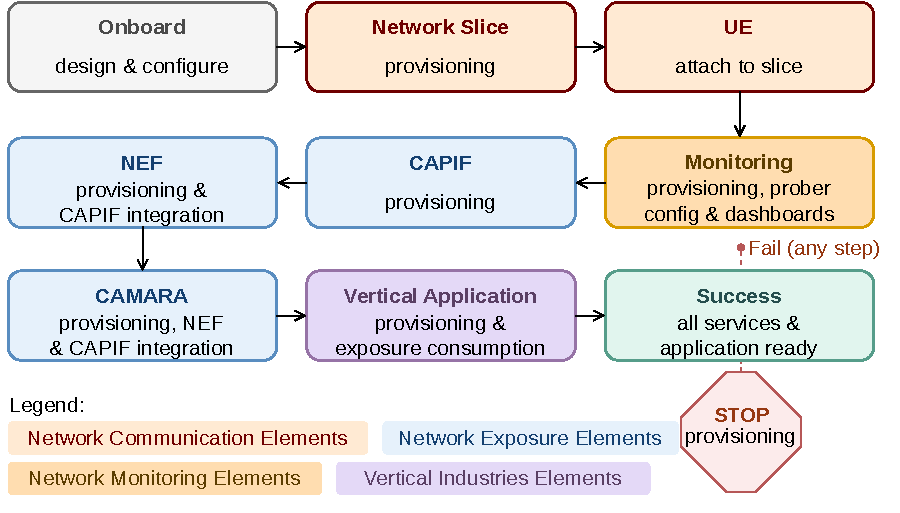
\includegraphics[width=0.8\linewidth]{figs/drawio/service_provisioning_chain.pdf}
    \caption{Sequential Orchestration Phases for a complete Network Application Experiment}
    \label{proposal:delivery:orchestration-lifecycle}
\end{figure}

Lastly, the runtime state of each experiment should be tracked through the \acs{TMF}~638 (Service Inventory Management) and \acs{TMF}~639 (Resource Inventory Management). The service inventory would record each service instance, its state and its relationships to other instances, allowing the \acs{OSS} to identify the dependent services to be created or terminated when an experiment is commissioned or decommissioned. The resource inventory would assume the equivalent role for the underlying resources, confirming that they are allocated on or released from the shared infrastructure.

\section{Multi-Vertical Use Case}
\label{chap:proposal:use-case}

To assess the testbed's suitability for the development and validation of vertical applications in an end-to-end scenario, a Network Application will need to be developed and evaluated in the proposed testbed. This will demonstrate the testbed's capabilities and showcase how its underlying infrastructure and interfaces can be used to deploy and validate applications under the requirements of a specific vertical use case. Section \ref{sota:networkapplications:usecases} highlighted several possible network applications across distinct verticals and scenarios, such as \ac{CAM}, \ac{TL}, and \ac{PPDR}. Given the testbed's goal of catering to multiple vertical industries, the considered \ac{PoC} targets the \ac{PPDR} and Automotive sectors through a vehicle collision detection and notification solution that bridges the two domains.

This use case is motivated by the need to improve the safety of road users in the moments immediately after an accident. Following a vehicle collision, involved and nearby vehicles and pedestrians remain exposed to the hazards of the crash site, increasing the risk of secondary incidents before emergency services arrive. Mitigating this risk requires detecting incidents quickly and immediately alerting those at and approaching the crash site. In this scenario, a computer vision model would analyze a live video stream from fixed roadside cameras to detect collisions and trigger notifications in real time, requiring close integration with the mobile network to automate detection and alerting.

\subsection{Application Interaction Flow}
\label{chap:proposal:use-case:flow}

Figure~\ref{fig:proposal:use-case-validation:flow:overview} illustrates a high-level view of the proposed solution and the interactions between its components. The envisioned system consists of three main elements: (i) a fixed roadside camera, acting as an \acs{UE}, that captures live video and streams it over the \acs{5G} network; (ii) an inference server, deployed at the edge or the cloud, that processes the received streams through an \acs{AI} vehicle collision detection model; and (iii) the actual network application that, through the northbound interfaces of the mobile network, manages the network resources supporting the video stream and alerts nearby road users once a collision is detected. In addition, operator dashboards should provide \acs{PPDR} agents with a real-time overview of the monitored road segment, displaying the live camera feeds alongside the detected collision events so they can inspect the scene and corroborate the outputs produced by the \acs{AI} model. Each event must be georeferenced and represented on an interactive map, together with the real-time positions of nearby road users. This information is also expected to be provided by the network.


\begin{figure}[htbp]
    \centering
    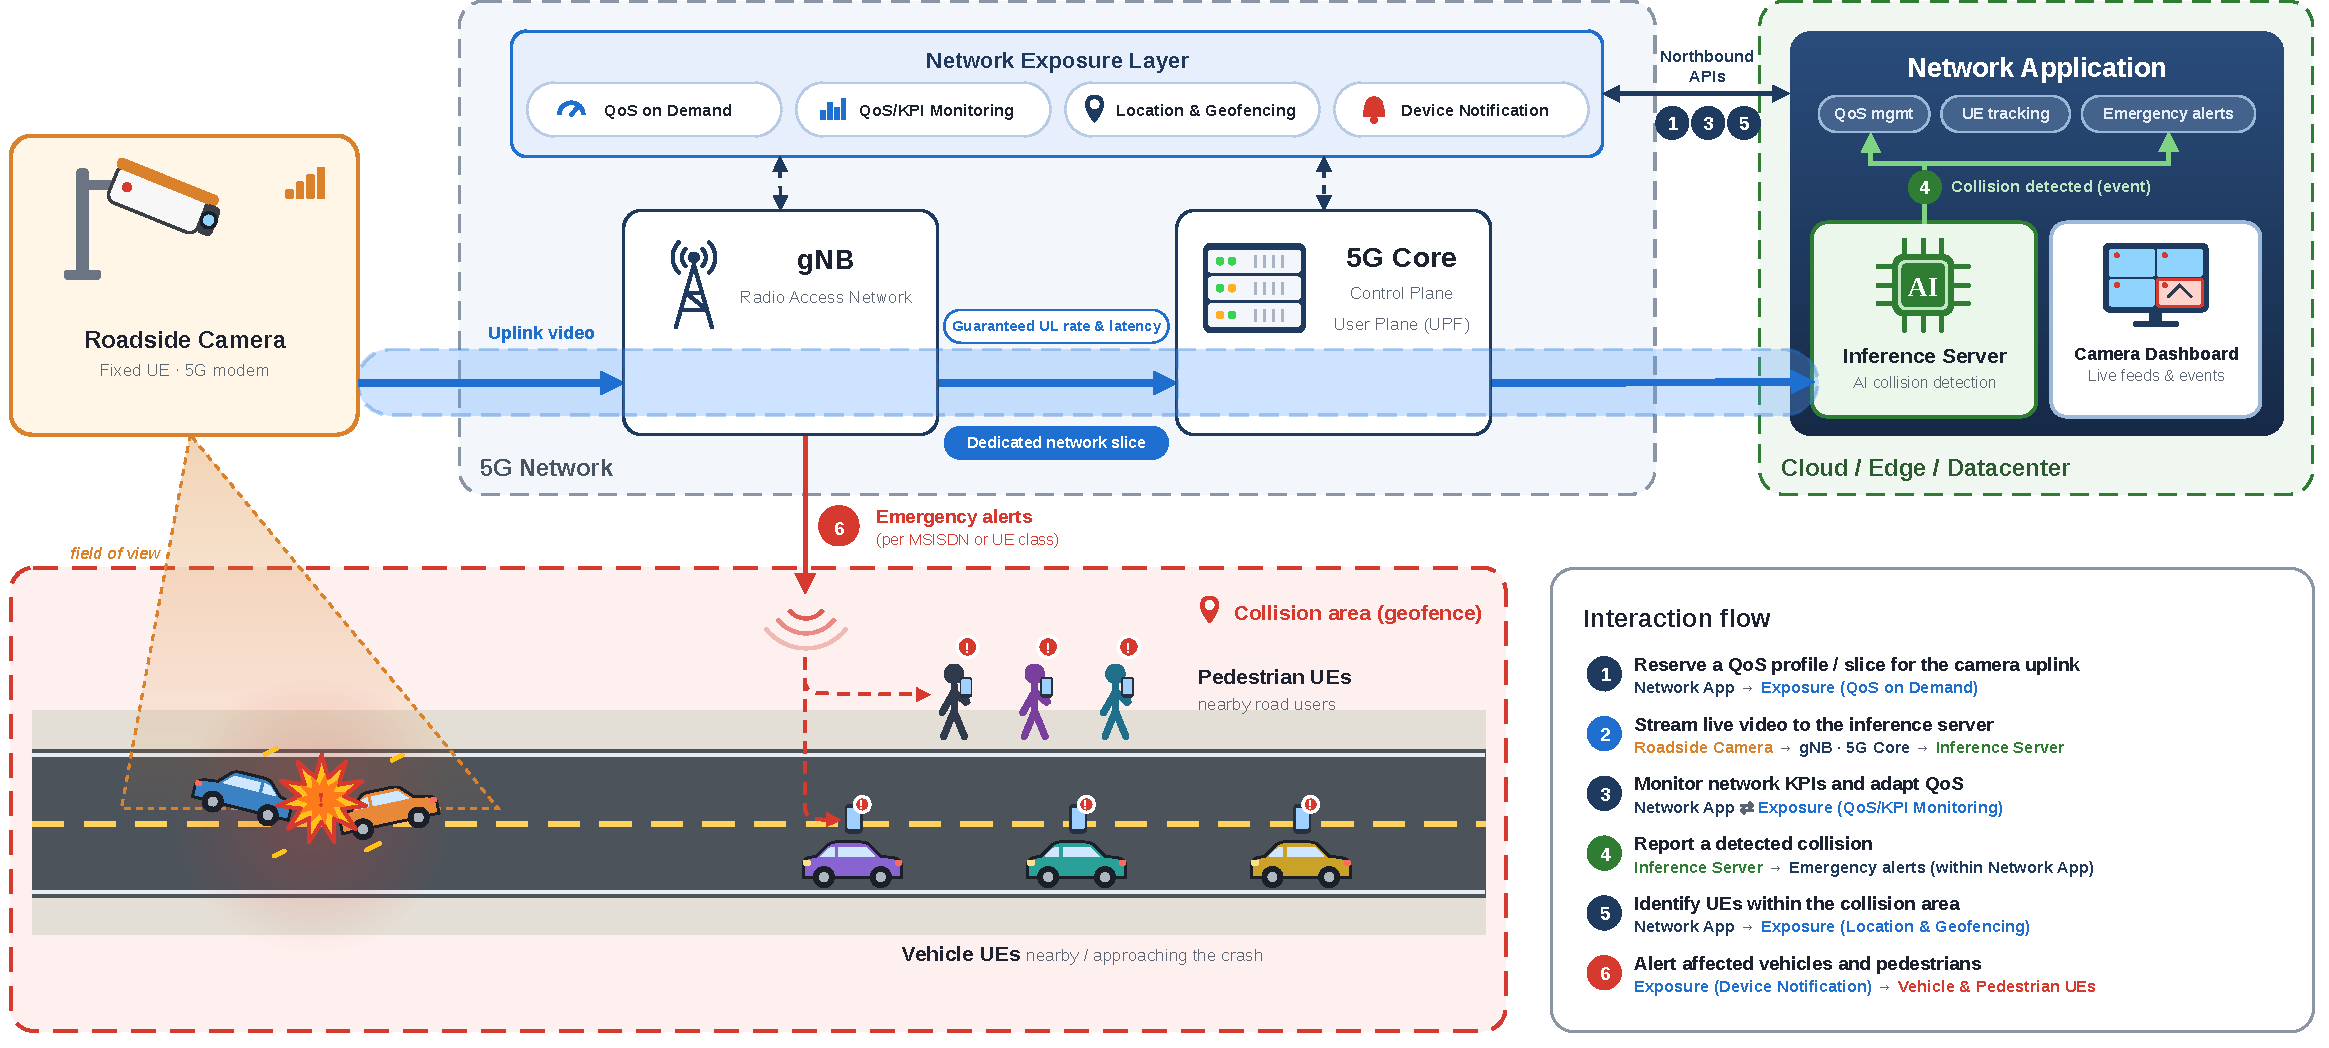
\includegraphics[width=1\linewidth]{figs/drawio/diagrama_napp.pdf}
    \caption{Conceptual overview of the proposed solution}
    \label{fig:proposal:use-case-validation:flow:overview}
\end{figure}



\subsection{Application Requirements}
\label{chap:proposal:use-case:requirements}

With the context and purpose of the network application established, the next step is to derive the requirements for the \acs{PoC} application. These will be organized into two categories: functional and non-functional requirements. Functional requirements describe the system and its functionality, i.e. the tasks it is capable of performing. Non-functional requirements specify the conditions under which the system is required to operate, as well as the properties it must exhibit. This category comprises performance requirements, which define the extent to which the system's functions must be executed through quantitative and individually verifiable metrics, and quality requirements, which capture system criteria such as security and portability.

\subsubsection{Functional Requirements}
\label{chap:proposal:use-case:requirements:functional}

The functional requirements align with the primary functionalities provided by the application. Given the emergency nature of the use case, stakeholders must be able to reserve the network resources needed to support the application. In particular, the uplink connection from the roadside camera to the inference server must satisfy defined throughput and latency requirements to ensure reliable, real-time detection. These requirements should be specified in advance, as part of the application's \acs{QoS} profile, and verified throughout the application's lifecycle. This requires continuous visibility into the network conditions experienced by the application, as the degradation of the communication layer may warrant, for instance, an adjustment of \acs{QoS} to preserve detection performance.

To achieve continuous monitoring and adaptive \acs{QoS}, the application requires exposure interfaces that allow it to interact programmatically with the underlying mobile network and request the necessary network capabilities and \acsp{KPI}. The same applies to other services that are crucial to its operation. The application must identify and track vehicle and pedestrian \acs{UE} within a defined perimeter around the monitored area, to determine which users to alert in case of an emergency. Once a collision is detected, these users must then be notified either individually, e.g. by \acs{MSISDN}, or collectively, by targeting a specific class of \acsp{UE}, such as those associated with pedestrians or vehicles. These capabilities, however, depend on the network infrastructure, and the testbed, exposing the necessary functionality to third-party applications through appropriate interfaces. Accordingly, the functional requirements of the application are defined as follows:

\begin{custenumerate}{FR}
    \item \label{enum:fr:slice} The system shall request, prior to its operation, the reservation of network resources dedicated exclusively to the application, isolated from other traffic sharing the mobile network, according to custom \acs{QoS} connectivity requirements;
    \item \label{enum:fr:stream} The system shall establish a live video stream from the roadside camera to the inference server over the \acs{5G} network;
    \item \label{enum:fr:detection} The system, i.e. the inference server, shall analyze each frame received from the video stream to detect vehicle collisions;
    \item \label{enum:fr:detection-event} The system shall report each detected vehicle collision as an event from the inference server to the network application;
    \item \label{enum:fr:dashboard} The system shall provide \acs{PPDR} agents with an operator dashboard presenting a real-time overview of the monitored road segment, including the live video stream from the roadside camera;
    \item \label{enum:fr:dashboard-collisions} The system shall display each detected vehicle collision on the operator dashboard, georeferenced on an interactive map;
    \item \label{enum:fr:qos-profile} The system shall reference a \acs{QoS} profile for the camera's data session, specifying the uplink throughput and latency to be requested from the network;
    \item \label{enum:fr:monitoring-profile} The system shall define a monitoring profile for the camera's data session, specifying the throughput and latency thresholds against which the observed network conditions should be evaluated;
    \item \label{enum:fr:qos-request} The system shall request the network \acsp{KPI} specified in the referenced \acs{QoS} profile for the camera's data session;
    \item \label{enum:fr:monitoring} The system shall monitor the network conditions experienced by the camera's data session, comparing them against the thresholds defined in the monitoring profile;
    \item \label{enum:fr:qos-change} The system shall change the active \acs{QoS} profile of the camera's data session whenever the monitored network conditions violate the thresholds defined in the monitoring profile;
    \item \label{enum:fr:ue-tracking} The system shall identify and actively track all vehicle and pedestrian \acsp{UE} in the vicinity of the surveilled area, displaying their real-time positions on the operator dashboard;
    \item \label{enum:fr:geofencing} The system shall detect all vehicle and pedestrian \acsp{UE} located within or entering a predefined area around the surveilled area;
    \item \label{enum:fr:notify-pedestrians} The system shall notify all pedestrian \acsp{UE} located within the predefined area identified in \ref{enum:fr:geofencing}, at the moment the collision detection event is processed;
    \item \label{enum:fr:notify-vehicles} The system shall notify all vehicle \acsp{UE} located within the predefined area identified in \ref{enum:fr:geofencing}, at the moment the collision detection event is processed;
    \item \label{enum:fr:notify-periodic} The system shall periodically reissue alert notifications to the appropriate \acsp{UE} until the incident is deemed resolved.
\end{custenumerate}

\subsubsection{Non-Functional Requirements}
\label{chap:proposal:use-case:requirements:nonfunctional}

The non-functional requirements specify the operational constraints that govern the execution of the functionalities defined above. Among these, the performance requirements are presented first, each linked to the functional requirements specified in Section~\ref{chap:proposal:use-case:requirements:functional} whose execution it constrains:

\begin{custenumerate}{NFR}
    \item \label{enum:nfr:uplink-bitrate} The uplink connection between the camera and the inference server shall sustain a guaranteed minimum bitrate sufficient to deliver the video stream at a rate of at least 30 \acs{FPS} (\ref{enum:fr:stream}, \ref{enum:fr:qos-profile}, \ref{enum:fr:qos-request});
    \item \label{enum:nfr:frame-processing} The system, i.e. the inference server, shall process at least one out of every three consecutive frames of the 30 \acs{FPS} input stream, such that no more than two consecutive frames are skipped at any given time (\ref{enum:fr:stream}, \ref{enum:fr:detection});
    \item \label{enum:nfr:degradation-detection} The system shall detect a degradation of the network conditions below the requirements declared in the \acs{QoS} profile within 1 second of its occurrence (\ref{enum:fr:monitoring-profile}, \ref{enum:fr:monitoring});
    \item \label{enum:nfr:qos-enforcement} The system shall enforce the new \acs{QoS} profile within 1 second of the degradation being detected (\ref{enum:fr:qos-change});
    \item \label{enum:nfr:notification-time} The system shall notify the affected \acsp{UE} within 1 second of the collision detection event (\ref{enum:fr:detection-event}, \ref{enum:fr:notify-pedestrians}, \ref{enum:fr:notify-vehicles}).
\end{custenumerate}

It should be noted that the verifiability of some of the performance requirements listed above is not determined exclusively by the envisioned system, but also by the capabilities provided by the underlying mobile network. As the core functionality of the application is dependent on the streaming of a live video over \acs{5G}, the requirements on uplink bitrate (\ref{enum:nfr:uplink-bitrate}), and consequently the sustained 30~\acs{FPS} stream, can only be satisfied if the network is configured with a \acs{QoS} profile that defines the necessary resource guarantees, and if the network can actually fulfill it. Similarly, the timing requirements for monitoring (\ref{enum:nfr:degradation-detection}), \acs{QoS} adaptation (\ref{enum:nfr:qos-enforcement}) and notifications (\ref{enum:nfr:notification-time}) partially depend on the processing and response times of the northbound interfaces exposed by the testbed.

The remaining requirements address the quality attributes of the system, which are independent of a specific operational scenario. These are not tied to any individual function and are transversal to the entire system:

\begin{custenumerate}{NFR}
    \setcounter{enumi}{5}
    \item \label{enum:nfr:secure-exposure} All northbound \acs{API} interactions shall be discovered, authenticated and authorized through a single secure exposure layer;
    \item \label{enum:nfr:logging} The system shall log all positive detection events and interactions with network \acsp{API}, including \acs{QoS} and location changes, to support debugging and validation procedures;
    \item \label{enum:nfr:packaging} All application components shall be packaged as \acs{NFV} or containerized applications, deployable through the testbed's orchestration infrastructure.
\end{custenumerate}

\section{Testbed Capabilities}
\label{chap:proposal:capabilities}

The preceding sections defined the capabilities the proposed testbed should offer to verticals, organized into resource lifecycle management, network exposure, network observability and service delivery. This section consolidates these capabilities and maps them to the \acs{PoC} functional and non-functional requirements gathered in Section~\ref{chap:proposal:use-case:requirements}, thereby illustrating how the testbed proposed capabilities support the practical needs of real-world vertical use cases. Table~\ref{tab:proposal:capabilities} summarizes this mapping.

As established in Section~\ref{chap:proposal:delivery}, at the top level, the testbed should provide a single management and automation platform (an \acs{OSS}) through which experimenters can order and manage all testbed functionality, exposed as services, via \acs{TMF} Open \acsp{API}. These services comprise the network slices and \acsp{UE} supporting the experiment, the exposure \acsp{API}, the monitoring services, and the network application itself. The platform would then delegate each service order to the appropriate orchestration and management platforms, following the dependency chain defined in that same section. In particular, the orchestration of the corresponding workloads, either as containerized or virtualized resources, would in turn fulfill the portability and deployment constraint imposed by \ref{enum:nfr:packaging}.

Initially, the testbed should provision the network slices that establish the connectivity conditions for the collision detection service, following the management hierarchy described in Section~\ref{chap:proposal:resource_lifecycle}, composed of the \acs{CSMF}, \acs{NSMF} and \acs{NSSMF}. This approach reserves the resources required by the \acs{PoC} before its operation, according to the \acs{QoS} requirements specified by the experimenter, i.e. the uplink requirements to support the camera video stream. Once the slice is deployed, the roadside camera \acs{UE} would be associated with it, so that its traffic is suject to the \acs{QoS} constraints defined for that slice. In doing so, the testbed addresses the application's requirement for dedicated and isolated network resources (\ref{enum:fr:slice}), theoretically guaranteeing the uplink bitrate required to sustain the live video stream from the camera to the inference server (\ref{enum:fr:stream}, \ref{enum:nfr:uplink-bitrate}).

Once the full experiment is provisioned, the application can take advantage of the network's capabilities through the exposure layer described in Section~\ref{chap:proposal:exposure}. These capabilities should be offered at two abstraction levels, by the \acs{NEF} and CAMARA \acsp{API}, and accessed through a single framework responsible for their secure publication, discovery and invocation, i.e. \acs{CAPIF}. This avoids application developers from the burden of interacting with distinct authentication servers for each exposure component, providing a unified approach to authentication and authorization (\ref{enum:nfr:secure-exposure}).

Application requirements related to the camera's data session, location services, and geofencing can be addressed through these northbound interfaces, independently of the exposure model. However, both altenra


Once the full experiment is provisioned, the application can take advantage of the network's capabilities through the exposure layer described in Section~\ref{chap:proposal:exposure}. Application requirements concerning the camera's data session, location services and geofencing procedures can be supported by the testbed's northbound \acsp{API} at two abstraction levels: \acs{NEF} and CAMARA \acsp{API}. Although both alternatives can accommodate the intended use case, they differ in terms of how comprehensively they can support each of the specified requirements, as showcased in Table~\ref{tab:proposal:capabilities}. More specifically, some functionalities, such as 

\later{to be completed}

. These capabilities should be offered at two abstraction levels, by the \acs{NEF} and CAMARA \acsp{API}, and


accessed through a single framework responsible for their secure publication, discovery and invocation, i.e. \acs{CAPIF}.


This relieves application developers from the burden of interacting with a separate authentication server for each exposure component, providing a unified approach to authentication and authorization (\ref{enum:nfr:secure-exposure}).


It also revelasl that 

specifying the actual northbound \acsp{API} that will be supporting network applications

At runtime, the application would interact with the network through the exposure layer described in Section~\ref{chap:proposal:exposure}. All \acs{NEF} and CAMARA \acsp{API} should be published, discovered and invoked through \acs{CAPIF}, providing the single secure exposure layer required by \ref{enum:nfr:secure-exposure}. Through these interfaces, the application would declare the \acs{QoS} and monitoring profiles of the camera's data session (\ref{enum:fr:qos-profile}, \ref{enum:fr:monitoring-profile}), request and change the active \acs{QoS} profile (\ref{enum:fr:qos-request}, \ref{enum:fr:qos-change}) and subscribe to network analytics on the experienced network conditions (\ref{enum:fr:monitoring}). Device location retrieval, verification and geofencing notifications would, in turn, allow the application to identify and track the road users within the surveilled area (\ref{enum:fr:ue-tracking}). The time limits imposed on degradation detection (\ref{enum:nfr:degradation-detection}) and \acs{QoS} enforcement (\ref{enum:nfr:qos-enforcement}) would therefore depend directly on the response times of these interfaces.

The analytics conveyed through the exposure layer must be grounded on measurements collected by the observation layer described in Section~\ref{chap:proposal:observability}. Passive monitoring would characterize the throughput of the camera's uplink traffic, while active monitoring would measure latency or \acs{RTT}. Both are required to evaluate the network conditions against the throughput and latency thresholds of the monitoring profile (\ref{enum:fr:monitoring}, \ref{enum:nfr:degradation-detection}). Complementarily, application logs, resource metrics and monitoring dashboards should support the debugging and validation procedures targeted by \ref{enum:nfr:logging}, allowing the observed behavior of the application to be correlated with the requests issued through the exposure layer.

Beyond these general purpose capabilities, alerting road users once a collision is detected requires notification mechanisms not covered by the preceding sections. The testbed should therefore deliver messages to individual \acsp{UE}, e.g. via \acs{SMS} addressed by \acs{MSISDN}, and broadcast messages to all \acsp{UE} of a given class located within a geographical area. These mechanisms would fulfill the notification of pedestrians and vehicles (\ref{enum:fr:notify-pedestrians}, \ref{enum:fr:notify-vehicles}), including their periodic reissue (\ref{enum:fr:notify-periodic}), within the time limit of \ref{enum:nfr:notification-time}. Although motivated by the \acs{PoC}, they are not specific to it and would remain available to other applications. The remaining requirements, namely \ref{enum:fr:detection}, \ref{enum:fr:detection-event} and \ref{enum:nfr:frame-processing}, concern the internal logic of the application and are not mapped to any testbed capability.


\begin{table}[htb!]
% Fraction of \linewidth taken by the Capability column; Requirements fits one functional and one non-functional requirement per line, Use Case is as wide as its header and Realization takes the remaining width
\newcommand{\capfrac}{0.2890}
\newlength{\reqwidth}
\newlength{\nclabelwidth}
\newlength{\ucwidth}
\newlength{\realwidth}
\newcommand{\realization}[1]{\multicolumn{2}{>{\RaggedRight\arraybackslash}p{\dimexpr\realwidth+\arrayrulewidth-2\tabcolsep\relax}|}{\leavevmode#1}}
% Category rows shaded with the same gray tone of the remaining tables, with \catpad of extra padding above and below the text
\newlength{\catpad}
\setlength{\catpad}{3pt}
\newcommand{\category}[1]{\rowcolor{gray!15}\multicolumn{5}{|l|}{\rule[\dimexpr-\arraystretch\dp\strutbox-\catpad\relax]{0pt}{\dimexpr\arraystretch\ht\strutbox+\arraystretch\dp\strutbox+2\catpad\relax}\textbf{\textit{#1}}}}
\centering
\small
\renewcommand{\arraystretch}{1.3}
% Remove booktabs vertical padding so that the vertical rules join the horizontal ones
\setlength{\aboverulesep}{0pt}
\setlength{\belowrulesep}{0pt}
\settowidth{\nclabelwidth}{CAMARA}%
\settowidth{\ucwidth}{\textbf{Case}}%
\addtolength{\ucwidth}{4pt}%
\settowidth{\reqwidth}{FR00, NFR0}%
\setlength{\realwidth}{\dimexpr\linewidth-\capfrac\linewidth-\reqwidth-2\tabcolsep-\ucwidth-2\tabcolsep-6\arrayrulewidth\relax}%
\begin{tabular}{|>{\RaggedRight\looseness=-1\arraybackslash}p{\capfrac\linewidth}|l|>{\RaggedRight\arraybackslash}p{\dimexpr\realwidth-\nclabelwidth-4\tabcolsep\relax}|>{\raggedright\arraybackslash}p{\reqwidth}|@{}>{\centering\arraybackslash}m{\ucwidth}@{}|}
\toprule
\textbf{Capability} & \multicolumn{2}{l|}{\textbf{Realization}} & \textbf{Require-}\newline\textbf{ments} & \multicolumn{1}{@{}>{\centering\arraybackslash}p{\ucwidth}@{}|}{\textbf{Use}\newline\textbf{Case}} \\
\midrule
\category{Resource Lifecycle Management and Service Delivery} \\
\midrule
Service design, ordering, provisioning and \acs{LCM} & \realization{\acs{OSS}, accessible via a user interface and \acs{TMF}~Open\acsp{API}} & \ref{enum:fr:slice}, \ref{enum:nfr:packaging} & \checkmark \\
\hline
Provisioning of network slices with custom \acs{QoS} & \realization{Delegation to Slice management functions\newline (\acs{NSMF} and \acs{NSSMF})} & \ref{enum:fr:slice}, \ref{enum:nfr:uplink-bitrate} & \checkmark \\
\hline
Provisioning and association of \acs{UE} with provisioned slice & \realization{Delegation to Slice management functions\newline (\acs{NSMF} and \acs{NSSMF})} & \ref{enum:fr:slice}, \ref{enum:fr:stream} & \checkmark \\
\hline
Orchestration of containerized services & \realization{Delegation to container orchestration platform, e.g. kubernetes using its native \acs{API}} & \ref{enum:nfr:packaging} & \checkmark \\
\hline
Orchestration of virtualized \acs{NF} and applications & \realization{Delegation to an \acs{NFVO} via \acs{ETSI} \acs{SOL}005} & \ref{enum:nfr:packaging} & \\
\midrule
\category{Network Exposure} \\
\midrule
Secure \acs{API} publication, discovery and invocation & \realization{\acs{CAPIF}} & \ref{enum:nfr:secure-exposure} & \checkmark \\
\hline
Declaration of application network quality thresholds & CAMARA & Application Profiles~\cite{CAMARAapis} & \ref{enum:fr:qos-profile}, \ref{enum:fr:monitoring-profile} & \checkmark \\
\hline
\multirow{2}{=}{Configuring~\acs{QoS} session for a device} & \acs{NEF} & AsSessionWithQoS~\cite{ETSI_TS_129_522_V18_11_0,ETSI_TS_129_122_V18_8_0} & \multirow{2}{=}{\ref{enum:fr:qos-request},~\ref{enum:fr:qos-change}, \ref{enum:nfr:qos-enforcement}} & \multirow{2}{*}{\checkmark} \\
\cline{2-3}
& CAMARA & Quality on Demand~\cite{CAMARAapis} & & \\
\hline
\multirow{2}{=}{Subscription~to network analytics} & \acs{NEF} & AnalyticsExposure~\cite{ETSI_TS_129_522_V18_11_0} & \multirow{2}{=}{\ref{enum:fr:monitoring}, \ref{enum:nfr:degradation-detection}} & \multirow{2}{*}{\checkmark} \\
\cline{2-3}
& CAMARA & Connectivity Insights\newline Subscriptions~\cite{CAMARAapis} & & \\
\hline
\multirow{2}{=}{Device location and geofencing notifications} & \acs{NEF} & MonitoringEvent~\cite{ETSI_TS_129_522_V18_11_0,ETSI_TS_129_122_V18_8_0} & \multirow{2}{=}{\ref{enum:fr:ue-tracking}} & \multirow{2}{*}{\checkmark} \\
\cline{2-3}
& CAMARA & Device Location~\cite{CAMARAapis} & & \\
\hline
\multirow{2}{=}{Device reachability and roaming notifications} & \acs{NEF} & MonitoringEvent~\cite{ETSI_TS_129_522_V18_11_0,ETSI_TS_129_122_V18_8_0} & \multirow{2}{=}{--} & \\
\cline{2-3}
& CAMARA & Roaming Status,\newline Reachability Status~\cite{CAMARAapis} & & \\
\hline
Traffic steering and other \acs{3GPP} procedures & \acs{NEF} & TrafficInfluence, PfdManagement, among others~\cite{ETSI_TS_129_522_V18_11_0,ETSI_TS_129_122_V18_8_0} & -- & \\
\midrule
\category{Network Observability} \\
\midrule
Passive traffic monitoring & \realization{Autonomous collection of network metrics, e.g. session throughput (full set at Table~\ref{tab:proposal:observability:metrics})} & \ref{enum:fr:monitoring}, \ref{enum:nfr:degradation-detection} & \checkmark \\
\hline
Active monitoring & \realization{Active prober process, collecting metrics such as \acs{RTT}, Packet Loss and \acs{RTT} jitter} & \ref{enum:fr:monitoring}, \ref{enum:nfr:degradation-detection} & \checkmark \\
\hline
Monitoring Visualization & \realization{Dashboard visualization of collected \acsp{KPI}} & \ref{enum:nfr:logging} & \checkmark \\
\midrule
\category{Notification} \\
\midrule
Delivery of \acs{SMS} notifications to individual \acsp{UE} & \realization{Application-facing \acs{SMS} submission \acs{API}} & \ref{enum:fr:notify-pedestrians},~\ref{enum:fr:notify-periodic}, \ref{enum:nfr:notification-time} & \checkmark \\
\hline
Geographic message broadcast to vehicles & \realization{Location-based \acs{V2X} messaging service} & \ref{enum:fr:notify-vehicles},~\ref{enum:fr:notify-periodic}, \ref{enum:nfr:notification-time} & \checkmark \\
\bottomrule
\end{tabular}
\caption{Summary of the proposed testbed capabilities}
\label{tab:proposal:capabilities}
\end{table}


\section{Validation}
\label{chap:proposal:validation}

The validation of \acs{5G} network applications cannot be limited to the testing methodologies of conventional software systems. This evaluation must verify the application functions as intended and effectively utilizes the exposed \acs{5G} capabilities, just deployed as services. However, these aspects cannot be meaningfully assessed in isolation, since the behavior of a network application results from the interplay of multiple factors: (i) its internal logic, (ii) how it interacts with the network through the available exposure interfaces, and (iii) ultimately the network conditions and capabilities that are actually delivered by the \acs{5G} system as a result of these interactions. 

In real operational environments, these conditions are highly dynamic and variable, often deviating from what's expected by a given vertical application, due to factors such as traffic load and the shared physical infrastructure. Network applications must therefore be capable of adapting to such variability, which must also be accounted for during their validation. This includes testing the application under both optimal (high throughput, low latency and jitter, no packet loss, etc.) and degraded scenarios (congestion, jitter, packet loss, loss of connectivity, etc.). Only through such comprehensive testing is it possible to assess the robustness and performance of the application and to determine whether it can satisfy the defined \acsp{SLA} when deployed over a real \acs{5G} network.

To achieve this, two different validation approaches are suggested: (i) simulating network events at the network exposure layer to create controlled and reproducible test scenarios; or (ii) relying on a real \acs{5G} network to introduce network impairments, directly affecting the behavior of the application under test.

The first approach focuses on the validation of the application logic, and how the application should react to the events and responses returned by the \acs{5G} network. By emulating responses such as analytics values, event notifications, or the outcome of \acs{QoS} requests, a wide range of scenarios can be evaluated without having to reproduce them in the actual network. In fact, this approach does not even require the existence of a \acs{5GC} or a fully operational \acs{5G} network. Since the \acs{NEF} is the entry point to \acs{5G} network programmability, it can be adapted to provide such responses through its standardized \acsp{API}. Open-source solutions, such as NEFSim~\cite{NEFsim}, have been developed specifically for this purpose. This is especially valuable at early stages of development, to assess the functional validity of the application before it is exercised on the actual network. In addition, should this approach be adopted in the testbed, its benefits would extend to other available exposure capabilities that internally consume the \acs{NEF}, such as CAMARA \acsp{API}. Therefore, the same emulation model could be used to validate the interaction with the network, independently of the exposure model preferred by the application.

The second approach evaluates the application's behavior under real network conditions provided by a deployed \acs{5G} system, once again taking advantage of the flexibility and programmability offered by the testbed. Through the network exposure interfaces described earlier, experimenters can request the enforcement of specific network conditions, i.e. \acs{QoS} profiles, and establish different networking scenarios with distinct performance characteristics. Under each scenario, the application is expected to adapt its behavior to the conditions enforced by the network: under favorable profiles, it should fully exploit the available resources and meet its target \acsp{KPI}, whereas under degraded conditions it should react gracefully, for instance, by lowering its service level (e.g. streaming resolution) or requesting a higher-priority \acs{QoS} profile. 

Moreover, the testbed capabilities could also be used to deliberately induce adverse or changing network conditions the application is expected to withstand. By stress testing the network with competing traffic, through its active probing mechanism, the testbed can reproduce these conditions in the live network, effectively degrading the \acs{QoS} of the provisioned slice and reducing the bandwidth available to the application, without relying on changes to its \acs{QoS} profile.

This section outlines the plan for the validation of the vertical use case presented in Section~\ref{chap:proposal:use-case}, in the proposed testbed. This includes the complete flow required to validate the application, including the service provisioning process needed to order and deploy the application and the testbed's services, which is detailed first. Furthermore, by validating the network application and exercising the testbed's network exposure interfaces and capabilities under realistic conditions, the testbed itself will also be validated, demonstrating its ability to support the end-to-end deployment and operation of vertical applications.

\subsection{Service Delivery}
\label{chap:proposal:validation:delivery}

Service delivery is the first step of the experimentation process, ordering and provisioning the underlying environment for the evaluation of vertical applications. For the \acs{PoC}, this environment would be composed of multiple services offered by the catalog presented in Section~\ref{chap:proposal:delivery:design}. The experimenter would first onboard the network application, packaging the application backend, the inference server and the \acs{PPDR} operator dashboards as a Network Application service.

This service would declare dependencies on the experiment's remaining services, parameterized to the use case. The Network Slice service would configure a \acs{NEST} meeting the uplink bitrate and latency requirements of \ref{enum:nfr:uplink-bitrate}. The User Equipment service would register the camera \acs{UE}, attaching it to the provisioned slice. The Network Exposure service would include \acs{CAPIF}, the \acs{NEF}, and optionally CAMARA \acsp{API}, according to the chosen abstraction level. Finally, the Network Observability service would provision the observability dashboards and, optionally, a prober to actively monitor the camera. At this point, the validation should confirm that the characteristics exposed by the catalog services suffice to express the requirements of the experimenter, according to the service design proposed in Section~\ref{chap:proposal:delivery:design}.

The experiment would then be instantiated through a single service order, submitted through the \acs{GUI} of the \acs{OSS} or the \acs{TMF}~641 \acs{API}. The validation of this process consists of verifying that the \acs{OSS} provisions each service following the chain depicted in Figure~\ref{proposal:delivery:orchestration-lifecycle}, deploying each phase only once its prerequisites are active. Upon completion, the state of the service order and the service inventory, retrieved through the \acs{TMF}~638 and \acs{TMF}~641 \acsp{API}, respectively, should indicate that all configured services are active and that their relationships are properly registered. Similarly, the resource inventory (\acs{TMF}~639) should confirm the provisioning of the underlying resources, matching the parameters of the original order.

To ensure that the resources have been successfully provisioned, it is also necessary to verify that the delegated orchestrator has deployed the corresponding resources. For instance, for containerized services orchestrated, for example, by Kubernetes, this would involve confirming, through its native \acs{API}, that the expected pods were scheduled and that their containers are running and ready. This lower level resources should also reflect the attributes of the ordered service, e.g. those of the ordered \acs{NEST}. Nonetheless, the conformance of the network conditions delivered by the slice should be assessed separately, as described in Section~\ref{chap:proposal:validation:use-case}.

A failure in any phase should prevent the provisioning of subsequent services, and the termination of the experiment should remove all of them. Since all application components would be deployed through the \acs{OSS}, without manual intervention, validating these aspects also verifies~\ref{enum:nfr:packaging}. Furthermore, repeatedly instantiating the same services across multiple executions should yield equivalent service and resource inventories, demonstrating consistent provisioning and proving the reproducibility of the service delivery process.

\subsection{Multi-Vertical Use Case}
\label{chap:proposal:validation:use-case}

Once the required services have been provisioned, the envisioned network application for the multi-vertical use case will be exercised and validated end-to-end on the testbed. In particular, this validation seeks to evaluate how the testbed enables the application to request and enforce the capabilities and network conditions demanded by the use case, and whether it can correctly adapt its behavior as these conditions change.

As noted at the beginning of this section, the functioning of a network application results from the combined operation of three complementary components, all of which must be considered during validation: (i) the application itself, (ii) the exposure layer, formed by the \acs{NEF} and CAMARA services, and (iii) the underlying \acs{5G} network. The testbed should therefore provide experimenters with the evidence required to understand how these components interact in pursuit of the application's goals. This requires analyzing observability data (e.g. metrics, logs) collected at each point of the experimental chain and correlating them, so that the observed behavior of the application can be traced back to its causes. This allows experimenters to verify not only that each request issued by the application was accepted, but also that it translated into the expected network conditions, and that the application reacted to those conditions as intended. For example, when an experimenter orders a network slice, the provisioned slice is expected to deliver the throughput and latency expressed in the attributes of the ordered \acs{NEST}. Verifying these conditions involves comparing the requested \acs{QoS} values with the metrics collected for the experiment, including those obtained through active probing.

% \section{Chapter Summary}
\label{chap:proposal:summary}

The following Section details how the testbed and the introduced capabilities are implemented at the \acf{ITAv}.

\plan{
    \begin{enumerate}
        \item How will NEFSim, CAMARA APIs and CAPIF be packaged?
    \end{enumerate}
}


\chapter{Implementation}
\label{chap:implementation}

This chapter details how the proposed testbed and capabilities are implemented at \acs{ITAv}. The architecture of the implemented testbed is presented in Section~\ref{chap:impl:architecture}, identifying the concrete components responsible for each of the proposed capabilities and how they interact. The subsequent sections detail the implementation of each capability, following the order adopted in the proposal:~\acs{5G}~resource lifecycle management in Section~\ref{chap:impl:resource_lifecycle}, network exposure in Section~\ref{chap:impl:exposure}, network observability in Section~\ref{chap:impl:observability}, and service delivery in Section~\ref{chap:impl:delivery}. Section~\ref{chap:impl:capabilities} then summarizes the full set of capabilities offered by the testbed.

Finally, the multi-vertical use case defined in the proposal is implemented in Section~\ref{chap:impl:use-case}, demonstrating how verticals and the network application can interact with the \acs{5G} system through the exposed interfaces. This includes the provisioning of the required \acs{5G} resources, the enforcement of \acs{QoS} requirements, and the monitoring of network conditions to support application and network \acs{QoS} adaptation.

\section{Architecture}
\label{chap:impl:architecture}


\begin{figure}[tp]
    \centering
    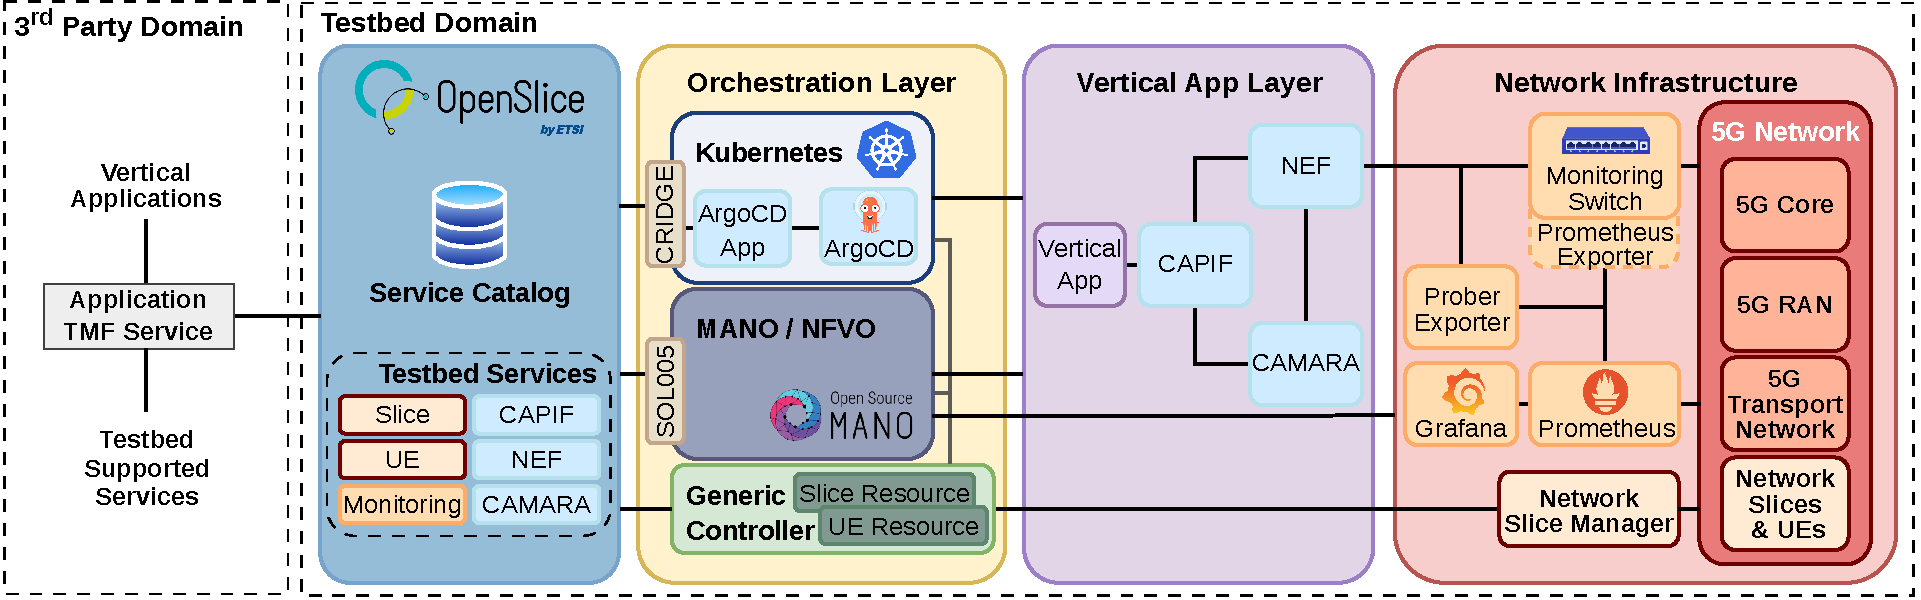
\includegraphics[width=1\linewidth]{figs/drawio/realized_architecture.pdf}
    \caption{Realized Testbed Architecture}
    \label{fig:impl:architecture}
\end{figure}

The proposed testbed is realized on the 5GAIner infrastructure~\cite{5GAIner} at \acs{ITAv}, which provides a commercial-grade standalone \acs{5G} network delivered through multiple \acs{5G} new radio cells and a Huawei \acs{5G} Core compliant with \acs{3GPP} Release 17. The testbed, illustrated in Figure~\ref{fig:impl:architecture}, implements the open, programmable environment proposed in Chapter~\ref{chap:proposal}, providing standardized interfaces to expose the network services offered by the infrastructure. It incorporates the \acs{5G} resource lifecycle management, network exposure, monitoring, and service provisioning capabilities highlighted in the proposal, identifying the concrete components that deliver each of the proposed functionalities. Combined, these components support the development and validation of applications by vertical industries and, consequently, of the exposure interfaces and underlying capabilities provided by the testbed.

Within the network exposure layer, the \acs{NEF}, proposed in Section~\ref{chap:proposal:architecture} as the main gateway for \acs{5G} programmability, establishes the foundation for the remaining exposure components. Due to the wide variety of \acs{5GC} implementations, an analysis of the various \acs{NEF} implementations was conducted in Section \ref{exposure:NEFimplementations}. Based on this analysis, the NEFSim~\cite{NEFSimMediaNetLabGithub}, as extended by \acs{ITAv}~\cite{NEFemulatorAtnog}, was selected as the most suitable choice for the \acs{NEF} implementation, due to its suite of supported northbound \acsp{API} and its integration capabilities with \acs{CAPIF} implementations, compared to its alternatives, as detailed in Section~\ref{chap:impl:exposure:nef}.

In order to further simplify the access to the complex set of network services offered by the NEFSim, CAMARA \acsp{API} are adopted, providing an abstraction layer that facilitates the integration of network capabilities into applications. This way, the CAMARA initative supports the development of network applications that explore the wide variety of use cases enabled through its set of user-friendly \acsp{API}, as described in Section \ref{sec:iniatives:CAMARA}.

Hence, the CAMARA and NEFSim components handle the exposure of network capabilities to third parties. However, there is still a lack of a standardized mechanism for the secure discovery, exposure, and consumption of these northbound \acsp{API}, which is achieved through the introduction of \acs{CAPIF}. More specifically, OpenCAPIF~\cite{OpenCAPIF}, an open source project by the \acs{ETSI} \acs{SDG}, was selected for the implementation of the \acs{CAPIF} framework, as detailed in Section~\ref{chap:impl:exposure:capif}. Thus, OpenCAPIF is utilized to securely expose CAMARA \acsp{API}, as well as \acs{NEF} \acsp{API}, to allow access to all \acs{NEF} functionalities not supported by the CAMARA use cases or that have previously been used for implementation within \acs{ITAv}.

The combination of OpenCAPIF, \acs{NEF} and CAMARA provides standardized secure access to network capabilities across a wide range of use cases. To support this variety of use cases, network slicing is applied to tailor to its heterogeneous service requirements on a common underlying infrastructure. To this end, \acf{OSL}~\cite{OpenSlice} is chosen as the predilect \acs{OSS} to deliver \acs{NaaS}, based on \acs{TMF} \acs{ODA}, since it is widely used in the literature for the provisioning and orchestration of \acs{5G} resources (especially \acsp{UE} and network slices) packaged as \acs{OSL} services, important for testing and validation purposes as showcased in Section \ref{sec:pipelines}. Service orders made to \acs{OSL} are fulfilled by the orchestration layer, being delegated to the \acs{NFVO} \acs{OSM}, for \acs{NFV}-based deployment through the SOL005 interface, or to kubernetes, for containerized deployment through the CRIDGE component. Services packaged as Helm charts, such as the vertical applications, are deployed on kubernetes through Argo CD. The \acs{NSMF} and \acs{NSSMF} roles defined in the proprosal are abstracted by the proprietary \acs{ITAv} Slice Manager, which provisions network slices and \acsp{UE} on the \acs{5G} system. \acs{OSL}, inspired by the Operator Pattern, also supports Generic Controllers to automate the lifecycle management of custom resources~\cite{OpenSliceGenericServicesController}. These are leveraged to implement the lifecycle logic for the \acs{NSI} as discussed in Section \ref{sec:slice:lifecycle}, as well as that of the \acsp{UE}. Such Generic Controllers are responsible for the creation, update and deletion of the aforementioned resources in the 5GAIner testbed by interacting with the Slice Manager, which in turn interacts with the \acs{5G} System (\acs{5GC} and \acs{RAN}), as detailed in Section~\ref{chap:impl:resource_lifecycle}.

It is also important to note the existence of a telemetry monitoring stack utilizing Prometheus exporters and Grafana for the collection and visualization of network metrics, respectively, as defined in Section~\ref{chap:proposal:observability}. Passive monitoring relies on a Prometheus exporter collecting traffic metrics from the \acs{5G} network, while active monitoring relies on a prober exporter measuring \acs{RTT}, packet loss and \acs{RTT} jitter. The collected metrics are stored in Prometheus, acting as the testbed's \acs{TSDB} for storing and querying network analytics. 

The result is an open, programmable environment in which vertical industries can develop and validate applications that interact with the \acs{5G} system.

\section{\acs{5G} Resource Lifecycle Management}
\label{chap:impl:resource_lifecycle}

As established in Section~\ref{chap:proposal:resource_lifecycle}, network slicing is the main mechanism that allows the testbed to support diverse vertical use cases and network applications, and their respective heterogeneous \acs{QoS} requirements. Delivering this requires the automation and orchestration of each phase of the \acs{NSI} lifecycle, a responsibility handled by the coordinated operation of the \acs{CSMF}, \acs{NSMF} and \acs{NSSMF} management functions. In this section, the components responsible for realizing each of these management functions are identified. However, in practice, not all of these functions have a direct counterpart within the implementation developed in this dissertation, being instead abstracted by other components already present in the \acs{ITAv} 5GAIner testbed~\cite{5GAIner}.

At the top of this management hierarchy, the \acs{OSL} \acs{OSS}~\cite{OpenSlice} is responsible for the \acs{OAM} functionality within the testbed, fulfilling the \acs{CSMF} role established in Section~\ref{chap:proposal:resource_lifecycle}. In this capacity, it exposes communication services to third-party clients through \acs{TMF} Open \acsp{API}, allowing them to request and provision \acs{5G} resources (network slices and \acsp{UE}) without requiring privileged knowledge of the underlying infrastructure. This abstraction is implemented by leveraging the \acf{CFS}, \acf{RFS} and Resource constructs, defined by \acs{TMF}, as mentioned in Section~\ref{sota:telcoinitiatives:tmf}. More concretely, each \acs{CFS} is exposed to customers as a configurable interface, through which clients can specify their desired service parameters (e.g. uplink throughput for a slice). Internally, the fields of the \acs{CFS}, expressing the user's requirements, are then mapped into a corresponding \acs{RFS} which in turn references the concrete Resource capturing the technical parameters required to provision the underlying network slice or \acs{UE}.

However, as previously discussed, \acs{OSL} is not an orchestrator, meaning the provisioning of the resources referenced by each \acs{RFS} is delegated to dedicated components. Therefore, \acs{OSL}, can delegate the provisioning of \acs{NFV} resources, to \acs{NFV} \acs{OSM}, via the SOL005 interface. Containerized resources, such as network applications, can also be automatically deployed to kubernetes through the CRIDGE component. In the case of network slices and \acsp{UE}, the provisioning of resources is delegated to a proprietary Slice Manager within \acs{ITAv}'s testbed.

This proprietary Slice Manager represents the primary mechanism for interacting with the \acs{5G} System, both the \acs{RAN} and the core, to provision network slices and \acsp{UE} in the 5GAIner infrastructure. This component abstracts the underlying complexity of interacting with the \acs{5G} System and \acs{NFV} infrastructure behind a unified \acs{API}, simplifying the management of \acs{5G} resources. Given the abstraction provided by this \acs{API}, the design and implementation of the \acs{NSMF} and \acs{NSSMF} services falls outside the scope of this dissertation, as their underlying functionality is already encapsulated within the Slice Manager. Consequently, \acs{OSL} must be capable of converting high-level customer service requirements, provided via a \acs{CFS}, into concrete \acs{API} calls to the Slice Manager, resulting in the provisioning of network slices and \acsp{UE}. This can be accomplished through the use of \acs{OSL} Generic Controllers~\cite{OpenSliceGenericServicesController}, which will be discussed in detail in the next section.

\subsection{Slicing Generic Controller}
\label{chap:impl:resource_lifecycle:controller}

A Generic Controller, inspired by the kubernetes operator pattern, is an \acs{OSL} component capable of managing resources of a specific type (of their resource specification)~\cite{OpenSliceGenericServicesController}. It is integrated natively into the OSL lifecycle, allowing custom code to be executed in response to the creation, update, and deletion of \acs{OSL} resources, by listening to a dedicated message queue for resource lifecycle events. This automated process allows the \acs{OSL} resources and services to be managed programmatically, ensuring they remain aligned with the state of the \acs{5G} deployment.

The Generic Controller\footnote{\url{https://github.com/Testbed-TNEI/SlicingGenericController}} developed in this dissertation was implemented using the Java Spring framework and manages two resource types: network slices and \acsp{UE}. For each resource type, a Resource Specification was defined, establishing the schema of the managed resource, aligned with the corresponding resource fields required by the Slice Manager \acs{API}. The controller runs as a standalone container, integrated with the \acs{OSL} deployment via its message queue. In this section, the design and implementation of the Generic Controller is presented, detailing how the controller converts the \acs{OSL} resource fields into Slice Manager \acs{API} calls for each resource type. It also describes how \acs{OSL} services are composed and structured into \acsp{CFS} and \acsp{RFS}, and addresses the integration of the testbed's observability mechanisms to monitor network slices and \acsp{UE} automatically upon provisioning.

\subsubsection{Network Slice Lifecycle Management}

The Slicing Generic Controller manages the lifecycle of network slice resources in the testbed. Each slice resource is defined by a Resource Specification capturing the parameters required for provisioning the resource using the Slice Manager \acs{API}. The required payload is provided in Appendix~\ref{appendix:slicemanager:payloads}, Code Block~\ref{code:slicemanager:payloads:netslice}, and its most relevant parameters include:

\begin{itemize}
    \item \texttt{id} \texttt{|} \texttt{name}: uniquely identify the slice resource in the \acs{5G} System;
    \item \texttt{administrative\_state} \texttt{|} \texttt{operational\_state}: indicate the slice status, regarding service (\texttt{LOCKED}, \texttt{UNLOCKED} or \texttt{SHUTTINGDOWN}) and operational state (\texttt{ENABLED} or \texttt{DISABLED}), respectively. The former controls whether the slice is available for use, while the latter its actual runtime condition and if it's capable of receiving traffic;
    \item \texttt{sst} \texttt{|} \texttt{ssd}: collectively form the \acs{S-NSSAI} identifier, classifying the slice type (e.g. \acs{eMBB}) and differentiating between slices of the same type, respectively;
    \item \texttt{dnn}: identifies the name of the target data network for the network slice;
    \item \texttt{dllatency} \texttt{|} \texttt{ullatency} \texttt{|} \texttt{dlguathptperue} \texttt{|} \texttt{ulguathptperue} \texttt{|} \texttt{dlmaxthpt\-perue} \texttt{|} \texttt{ulmaxthptperue} \texttt{|} \texttt{dlguathptperslice} \texttt{|} \texttt{ulguathptperslice} \texttt{|} \texttt{dl\-maxthptperslice} \texttt{|} \texttt{ulmaxthptperslice}: define the \acs{QoS} performance requirements of the slice, covering downlink and uplink latency, guaranteed and maximum throughput per \acs{UE}, and guaranteed and maximum throughput of the slice, respectively.
\end{itemize}

The fields of the Resource Specification, illustrated in Figure~\ref{} and defined in Code Block ~\ref{} (at Appendix~\ref{}), are aligned with the parameters accepted by the Slice Manager \acs{API}, allowing the Generic Controller to directly incorporate the resource state into the corresponding \acs{API} payload. Upon resource creation, the Generic Controller receives the  corresponding \texttt{CREATION} message and issues a \texttt{POST} request to the \texttt{/productOrder} endpoint of the Slice Manager \acs{API}, instantiating the network slice across the \acs{RAN} and \acs{CN}. Update events trigger a \texttt{PATCH} request to the \texttt{/productOrder/\{id\}/patch} endpoint of the Slice Manager \acs{API}, including the slice id and the modified resource parameters to update the slice configuration according to the new client requirements. Deletion of the resource triggers a \texttt{DELETE} request to the \texttt{/productOrder/\{id\}} endpoint of the Slice Manager \acs{API}, resulting in the deprovisioning of the slice and disassociation of any linked \acsp{UE}, operations that are once again abstracted by the Slice Manager component.

\subsubsection{\acl{UE} Lifecycle Management}

The Slicing Generic Controller also manages the lifecycle of \acs{UE} resources, handling their configuration, instantiation and association with the provisioned network slices. Following the same pattern established for the network slice resource, each \acs{UE} resource is defined by a Resource Specification with the exact parameters required by the Slice Manager \acs{API} to manage \acsp{UE}. The corresponding payload is also provided in Appendix~\ref{appendix:slicemanager:payloads}, Code Block~\ref{code:slicemanager:payloads:ue}, and its most relevant parameters include:

\begin{itemize}
    \item \texttt{IMSI}: identifies the \acs{UE} within the \acs{5G} network through its \acf{IMSI};
    \item \texttt{slice}: references the identifier of the network slice with which the \acs{UE} is to be associated, linking the device to the corresponding provisioned slice;
    \item \texttt{IPV4} \texttt{|} \texttt{IPV6}: define the \acs{IP} addresses assigned to the \acs{UE} within the target slice, used for traffic routing and \acs{UE} telemetry collection by the monitoring stack;
    \item \texttt{AMBRUP} \texttt{|} \texttt{AMBRDW}: optionally define the Aggregate Maximum Bit Rate of the \acs{UE} in the uplink and downlink directions, across non-\acs{GBR} sessions, respectively.
\end{itemize}

Following the same approach as in the network slice case, the \acs{UE} Resource Specification incorporates the same fields as those required by the corresponding Slice Manager \acs{API} requests, as showcased in Figure \ref{} (and Code Block~\ref{} at Appendix~\ref{}). Similarly, upon resource creation, the Generic Controller receives the corresponding \texttt{CREATION} message and issues a \texttt{POST} request to the \texttt{/ue/post} endpoint of the Slice Manager \acs{API}, registering the \acs{UE} and associating it with the target slice specified in the \texttt{slice} field. Deletion of the resource triggers a \texttt{DELETE} request to the \texttt{/ue/\{imsi\}/delete\_IMSI} endpoint, which simultaneously handles the removal of the \acs{UE} and its disassociation from the corresponding slice. However, the Slice Manager \acs{API} does not expose a dedicated endpoint for modifying a given \acs{UE}, which means that updating the slice association of an active \acs{UE} or any of its fields is not directly supported under the current implementation of the slicing generic controller. Consequently, any modification to an active \acs{UE}, including a change to its slice association, requires deleting and recreating the corresponding resource, knowing that in an optimal setting, it should be possible to migrate a \acs{UE} between slices without this overhead.

\subsection{Service Composition}

The Slicing Generic Controller, as any \acs{OSL} Generic Controller, manages the network slice and \acs{UE} entities at the resource level, representing the lowest layer of the \acs{TMF} hierarchy previously described, i.e. Product, Service and Resource. To make these resources configurable and available through the \acs{OSL} service layer and \acs{TMF} \acsp{API}, corresponding \acsp{RFS} are defined for each resource type, encapsulating the resource and inheriting all its fields as configurable parameters. By leveraging the Network Slice and \acs{UE}'s \acs{RFS}, presented in Figures \ref{} and \ref{}, operators or anyone designing services in \acs{OSL} possess all the means necessary to provision and manage network slices and the associated \acsp{UE}.

To expose these network slice and \acs{UE} management capabilities to third-party clients, \acsp{CFS} can be defined, namely a Network Slice \acs{CFS} and a UE \acs{CFS} composed by the corresponding \acsp{RFS}, each built on top of the respective \acsp{RFS}. This way, the service designer has control over which parameters are configurable through the \acs{CFS}, ensuring that only the fields relevant to the intended use case are exposed to customers. However, since \acs{CFS} and \acs{RFS} are distinct service constructs within \acs{OSL}, \acs{LCM} rules are required to keep them synchronized and ensure the \acs{OSL} state accurately reflects the state of the Slice Manager and, consequently, of the \acs{5G} System. Any changes to the customer requirements, defined via the \acs{OSL} \acs{CFS} fields, must be propagated downwards to the corresponding \acs{RFS} fields, triggering resource provisioning via the Generic Controller and corresponding Slice Manager \acs{API} call. Similarly, once the Slice Manager processes the request, the Generic Controller must update the corresponding resource fields based on the response, whether the operation was successful or not. In the event of a failure, this may involve rolling back the customer changes and displaying a user-friendly error message. The resulting state is then propagated upwards to the \acs{CFS} via \acs{LCM} rules, ensuring the \acs{OSL} service state remains consistent with the actual network state and that the result is reported back clearly to the user.

In this dissertation, three \acs{CFS} specifications are developed to address the management of network slices and \acsp{UE}, which are presented in Figure \ref{}. A standalone Network Slice \acs{CFS} and a standalone \acs{UE} \acs{CFS} are provided for the independent management of each resource type. Additionally, a bundled Network Slice and \acs{UE} \acs{CFS} groups the provisioning of a network slice and one associated \acs{UE} into a single service request. In both the Network Slice and Bundled \acs{CFS}, the network slice \texttt{id} is automatically generated (\acs{UUID}) by \acs{OSL}, before provisioning it through the Slice Manager \acs{API}. For the standalone \acs{UE} \acs{CFS}, the Generic Controller must additionally validate that the referenced network slice exists and that its maximum number of \acsp{UE} isn't exceeded by associating this additional \acs{UE}.


\subsection{Observability Integration}

As established in Section~\ref{chap:proposal:observability}, a core objective of the testbed is to deliver a fully automated monitoring process that can operate without manual human intervention. For this goal to be accomplished, the monitoring procedures must be directly integrated into the provisioning lifecycle managed by \acs{OSL}, ensuring that telemetry dashboards and/or collection are automatically enabled and disabled according to the lifecycle of each slice and \acs{UE} resource, and their parameters (e.g. \acs{UE} \acs{IP} or \acs{MAC} address). The underlying observability components responsible for collecting and exposing these metrics are described in detail in Section~\ref{chap:impl:observability}. This section focuses on how their integration is implemented with the developed Slicing Generic Controller and \acs{OSL}.

Once a network slice (service) is ordered in \acs{OSL}, a Grafana dashboard is automatically provisioned, scoped to that slice and its associated \acsp{UE}. This is achieved through a \texttt{PRE\_PROVISION} \acs{LCM} rule which triggers a Jenkins pipeline that deployes a Grafana Helm chart, pre-configured with a Prometheus data source (responsible for storing passive monitoring metrics of the \acs{5G} network) and the corresponding slice dashboards exposing the relevant metrics, as showcased in Figure \ref{}. As \acsp{UE} are subsequently associated with or disassociated from the slice (when deleted), the dashboard is updated accordingly, ensuring that the dashboard metrics always reflect the current set of \acsp{UE} assigned to the slice.

In Section~\ref{chap:proposal:observability:activemonitoring} active probing was introduce as a complement to passive monitoring. However, this monitoring approach continuously generates synthetic traffic targeting provisioned \acs{UE}, introducing additional load on the network. Therefore, it is not appropriate for it to be mandatory for every slice and \acs{UE}. Thus, active probing is only activated when the customer explicitly requests it, by setting the \texttt{active\_probing} field to \texttt{true} in the Network Slice \acs{CFS}. Internally, this results in the Generic Controller performing an \texttt{UPDATE} request to an \acs{API} endpoint encapsulating the prober configuration file, also described in Section~\ref{chap:impl:observability}.

Similarly to the approach discussed in the previous section, any changes to the \acs{OSL} services must also be reflected in the corresponding observability procedures. After provisioning a new slice and respective grafana dashboard, newly provisioned \acsp{UE} trigger the extension of that dashboard and, where applicable, the registration of their \acs{IP} addresses with the probing container. When the \acs{OSL} \acs{UE} resource is deleted and the \acs{UE} deprovisioned, the corresponding entries are removed from the slice dashboard and any active probing sessions terminated. Finally, upon deleting the slice, the corresponding dashboard and grafana deployment should be deprovisioned. Should any of these operations not complete as expected, the outcome must be reported back to the client, with the \acs{OSL} service state always reflecting the latest active monitoring configuration.

\subsection{Slicing Management Interaction Flow}

The previous sections described the network slice and \acs{UE} resources managed by the Slicing Generic Controller, as well as their composition into \acs{OSL} services. This section details how each resource lifecycle event received from \acs{OSL}, more specifically from its service orchestration and order management component (OSOM), is translated into the corresponding Slice Manager \acs{API} operations. 

The current version of the Slice Manager \acs{API} adopts an asynchronous processing model, in which each write operation is accepted immediately and assigned a unique operation identifier, used to subsequently retrieve the execution outcome. Figure~\ref{fig:impl:resource_lifecycle:flow:sequence} illustrates the interaction sequence between the \acs{OSL} orchestrator and \acs{TMF} \acsp{API}, the Slicing Generic Controller and the Slice Manager, for the creation, update and deletion of network slice and \acs{UE} resources.

\begin{figure}[htbp]
    \centering
    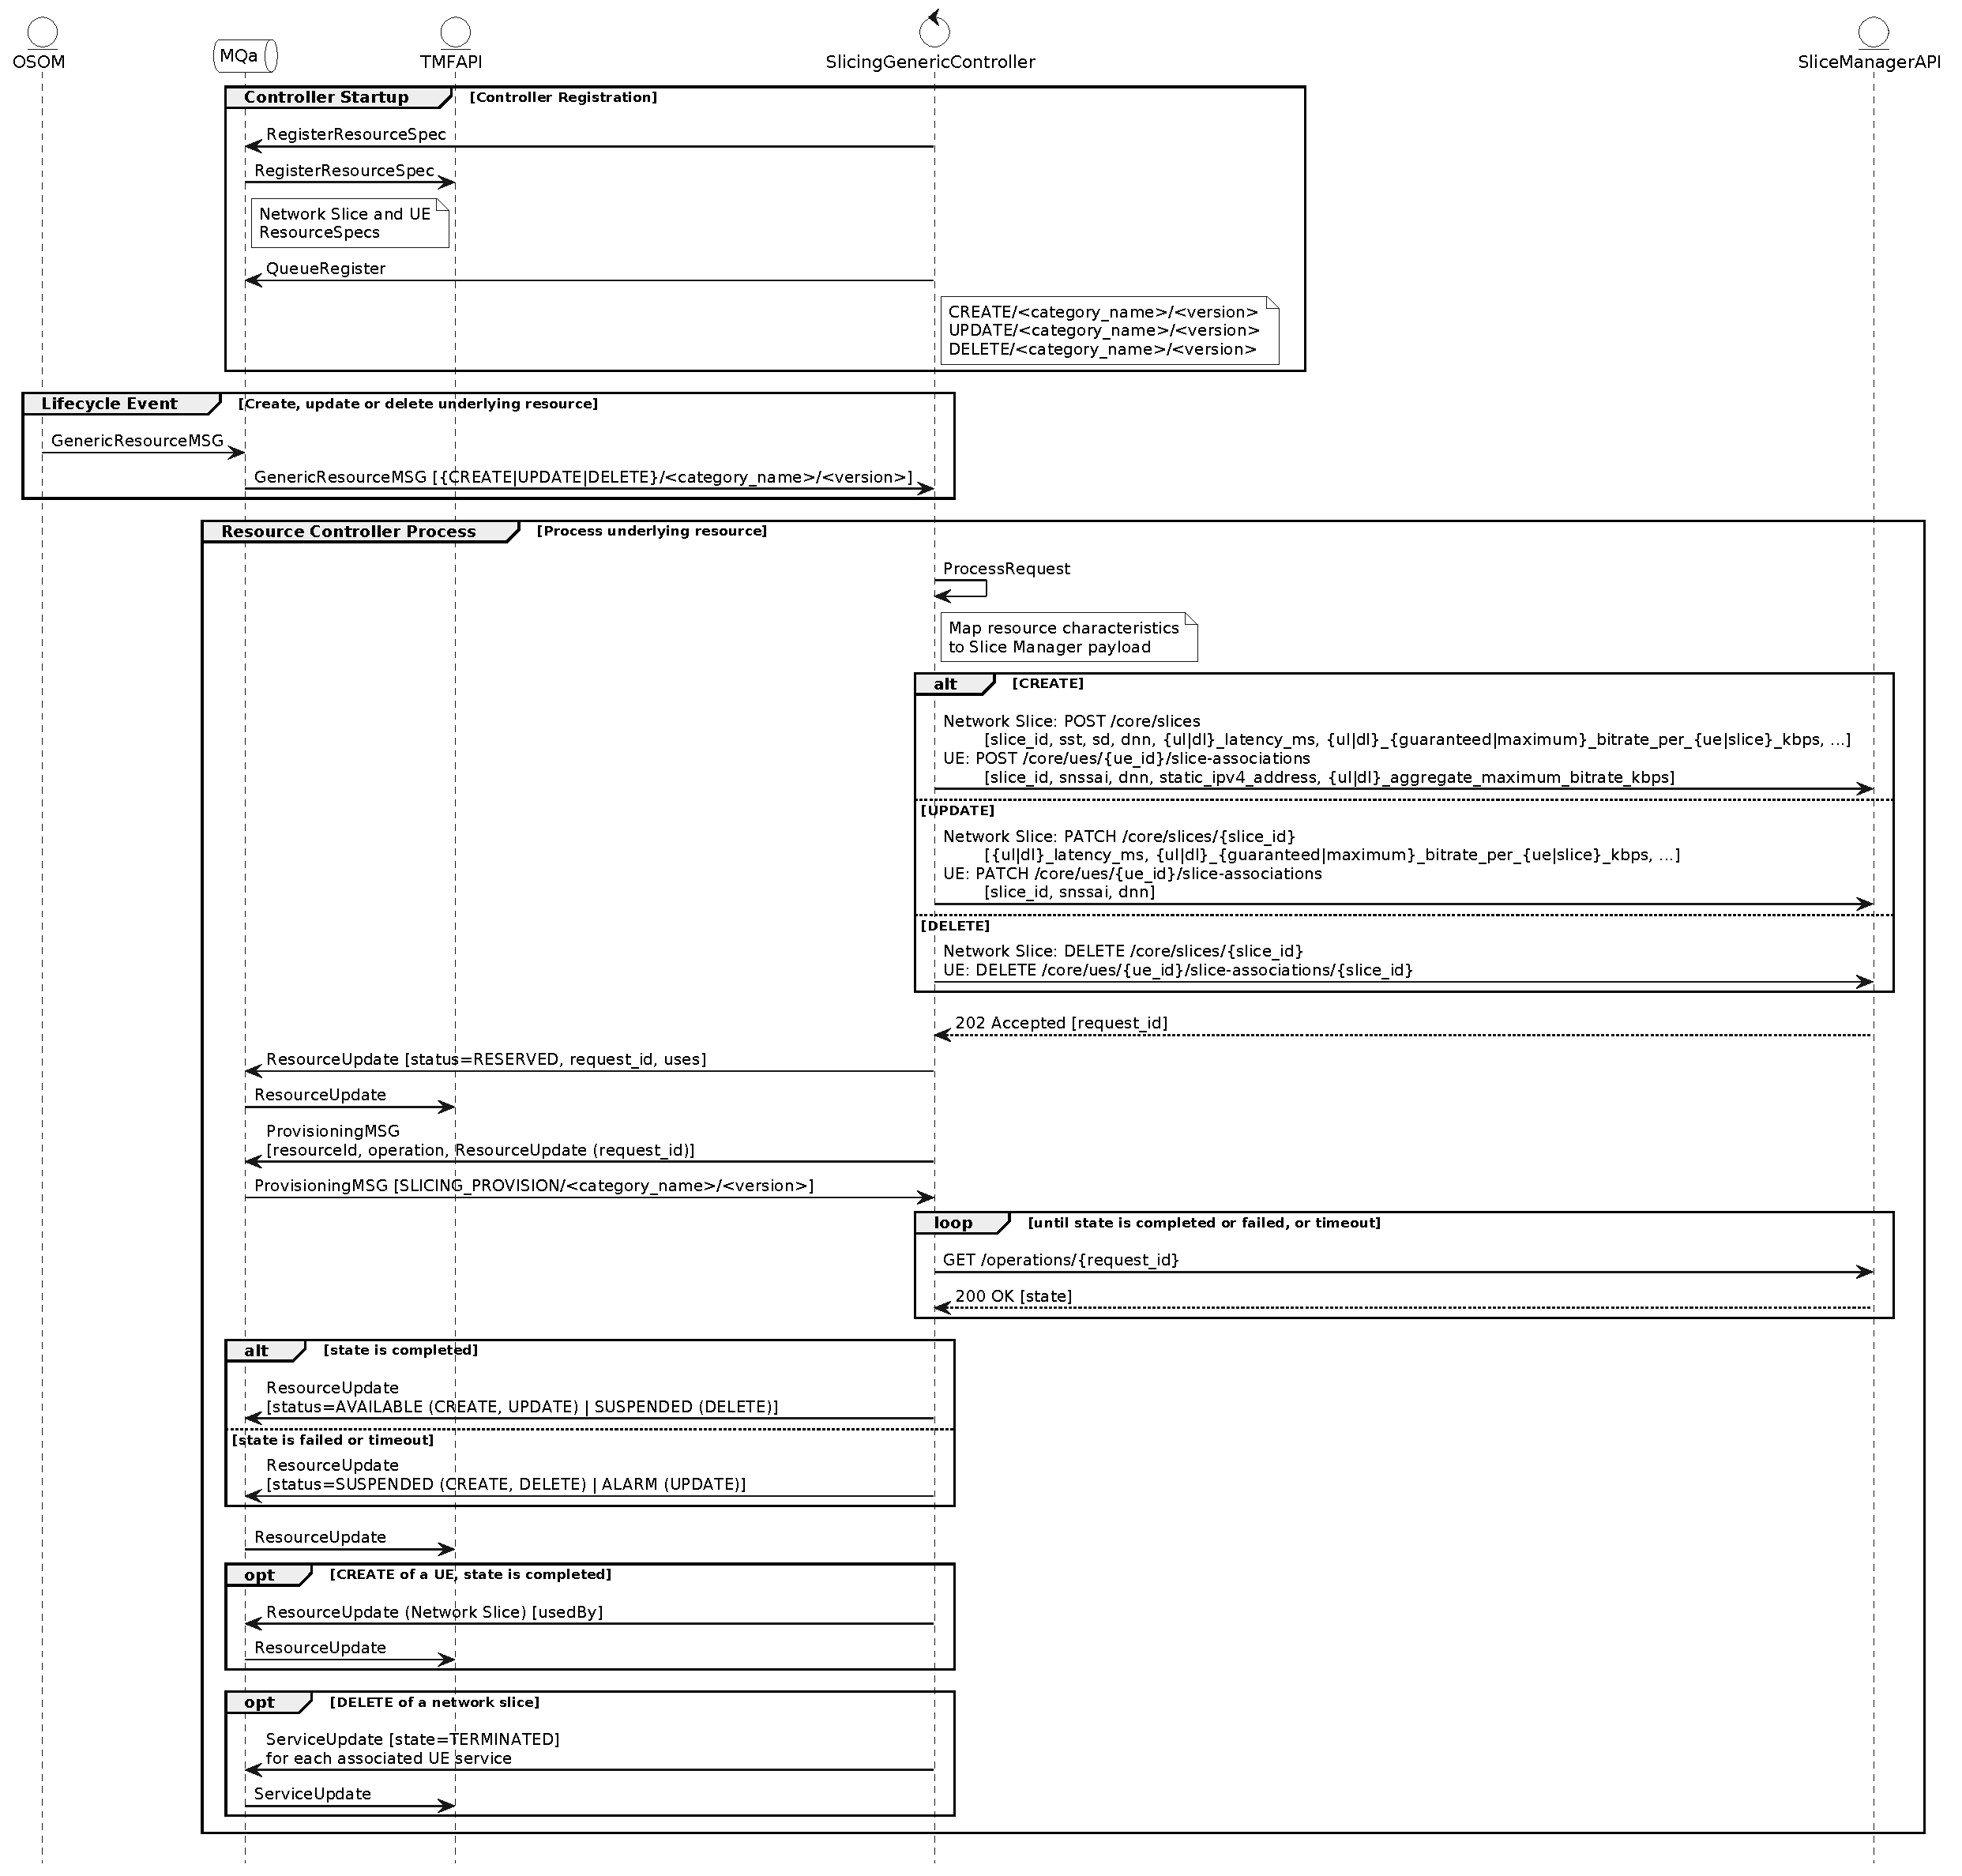
\includegraphics[width=1\linewidth]{figs/plantuml/slicing-gcontroller-lifecycle-sequence.pdf}
    \caption{Sequence Diagram for the \acs{LCM} of Network Slice and \acs{UE} Resources via the Slicing Generic Controller}
    \label{fig:impl:resource_lifecycle:flow:sequence}
\end{figure}

Before processing any lifecycle event, the controller registers with \acs{OSL} at startup (Controller Startup). Through the message queue, it registers the Network Slice and \acs{UE} Resource Specifications in \acs{OSL}, exposed by the \acs{TMF} \acsp{API}, subscribing to one separate queue per lifecycle event (\texttt{CREATE}, \texttt{UPDATE} and \texttt{DELETE}).

Each lifecycle event is delivered by OSOM to the corresponding queue, and received by the Generic Controller. The controller then maps the resource characteristics into the payload expected by the Slice Manager \acs{API}. The Slice Manager is therefore responsible for managing the lifecycle of network slices and their associations with \acsp{UE}, ensuring consistency across the various parts of the \acs{5G} system, e.g. \acs{5GC}, \acs{RAN}. In contrast, the Generic Controller serves as a synchronization layer between the \acs{OSL} \acs{TMF} resources and the state maintained by the Slice Manager.

In Figure~\ref{fig:impl:resource_lifecycle:flow:sequence}, the mapping between lifecycle events and Slice Manager endpoints is summarized in the first alternative block. A \texttt{CREATE} event results in a \texttt{POST} request to \texttt{/core/\allowbreak slices}, which provisions the network slice, or to \texttt{/core/\allowbreak ues/\allowbreak \{ue\_\allowbreak id\}/\allowbreak slice\allowbreak -associations}, which associates the \acs{UE} id, i.e. the \acs{IMSI}, with an existing slice. An \texttt{UPDATE} event results in a \texttt{PATCH} request to \texttt{/core/\allowbreak slices/\allowbreak \{slice\_\allowbreak id\}}, modifying the \acs{QoS} parameters of the slice in place while preserving its \acs{UE} associations, or to \texttt{/core/\allowbreak ues/\allowbreak \{ue\_\allowbreak id\}/\allowbreak slice\allowbreak -associations}, moving the \acs{UE} to another slice. Finally, a \texttt{DELETE} event results in a \texttt{DELETE} request to \texttt{/core/\allowbreak slices/\allowbreak \{slice\_\allowbreak id\}} or to \texttt{/core/\allowbreak ues/\allowbreak \{ue\_\allowbreak id\}/\allowbreak slice\allowbreak -associations/\allowbreak \{slice\_\allowbreak id\}}, removing the slice or the \acs{UE} association, respectively.

Throughout these operations, the Slice Manager performs the necessary interactions with the \acs{5G} System to provision or deprovision the requested resources. It is also responsible for ensuring the validity of each request, rejecting, for instance, the association of a \acs{UE} with a non-existent slice. Otherwise, the Slice Manager accepts the request with a \texttt{202 Accepted} response carrying an operation identifier (\texttt{request\_id}). The controller does not wait for the operation to complete before replying to OSOM, since OSOM treats a reply that exceeds its request timeout as a deployment failure, while the provisioning of a network slice may take considerably longer. Instead, the controller stores the operation identifier as a resource characteristic, sets the resource status to \texttt{RESERVED} through the \acs{OSL} \acs{TMF} \acsp{API}, and replies immediately.

The operation is then published to a persistent queue (\texttt{SLICING\_\allowbreak PROVISION}), scoped by the same category and version, and consumed by a dedicated polling service within the controller. Messages in this queue are only acknowledged once the final resource status is written back to \acs{OSL}, so a controller restart results in the redelivery of pending operations rather than in resources left indefinitely in the \texttt{RESERVED} state. Furthermore, messages are grouped by resource identifier, ensuring that operations targeting the same resource are processed in order, for example, preventing a deletion from overtaking the creation it cancels.

The polling service periodically queries the \texttt{/operations/\allowbreak \{request\_\allowbreak id\}} endpoint until the operation state is reported as either completed or failed, or until a predefined timeout elapses. Polling is required since the Slice Manager does not support callback endpoints. Based on the outcome, the controller updates the status of the \acs{OSL} resource, again through the \acs{TMF} \acsp{API}. Successful creations and updates set the resource to \texttt{AVAILABLE}, while successful deletions set it to \texttt{SUSPENDED}, allowing \acs{OSL} to transition the corresponding service to the \texttt{TERMINATED} state. Failed creations and deletions also set the resource to \texttt{SUSPENDED}, preventing OSOM from waiting indefinitely on an operation that will not complete. Failed updates, in turn, set the resource to \texttt{ALARM}, since the resource remains provisioned and carrying traffic, and deleting it would not revert the requested modification. In all cases, the outcome of the operation is stored as a resource characteristic, so that the result is reported back to the client through the \acs{OSL} service state.

To keep track of which \acsp{UE} are associated with each network slice, the controller also maintains relationships between the corresponding \acs{OSL} resources. Upon the creation of a \acs{UE}, a \texttt{uses} relationship referencing the target slice is added to the \acs{UE} resource, together with the \texttt{RESERVED} status, and, once the association completes, a reverse \texttt{usedBy} relationship referencing the \acs{UE} is added to the slice resource. Lastly, the deletion of a network slice implicitly removes all \acs{UE} associations in the Slice Manager. To keep the \acs{OSL} state consistent with the network, the controller sets the services of every \acs{UE} associated with the deleted slice to \texttt{TERMINATED}, which in turn triggers OSOM to send a \texttt{DELETE} message for each corresponding \acs{UE} resource and, consequently, the deletion of the resource.

\section{Network Exposure}
\label{chap:impl:exposure}

As outlined earlier, the \acs{NEF}, CAMARA and \acs{CAPIF} components form the standardized exposure layer of the testbed at the northbound of the \acs{5G} core. The implementation of each of these components is presented next.

\subsection{\acs{NEF}}
\label{chap:impl:exposure:nef}

As it has been repeatedly noted throughout this document, the \acs{NEF} is the primary network function of the \acs{5GC} \acs{SBA} responsible for the exposure of network capabilities to third parties. The testbed developed in this work follows the same principle, relying on the \acs{NEF} as the primary entry point for external interactions with the \acs{5GC}.

Based on the analysis of the available \acs{NEF} implementations conducted in Section~\ref{exposure:NEFimplementations}, the NEFSim~\cite{NEFsim}, as extended by \acs{ITAv}~\cite{NEFemulatorAtnog}, was selected as the most suitable choice for this role within the testbed. This selection was motivated by a variety of factors:

\begin{enumerate}
    \item \textbf{Wider coverage of \acs{NEF} northbound \acs{API} suite}~\cite{ETSI_TS_129_522_V18_11_0}\textbf{:} including the \textit{PfdManagement}, \textit{MonitoringEvent}, \textit{AsSessionWithQoS} and \textit{TrafficInfluence} \acsp{API} \fix{COMPLETE THIS};
    \item \textbf{Built-in Integration with \acs{CAPIF}:} among the analyzed implementations, it is the only one which supports, or even considers, authentication, authorization and service discovery capabilities, using the \acs{CAPIF} framework;
    \item \textbf{Simulated Environment:} the NEFSim exposes the standardized set of \acs{NEF} northbound \acsp{API}, allowing network application developers to develop and validate network applications, without requiring access to a fully featured \acs{NEF} instance;
\end{enumerate}

Hence, in its original purpose, the NEFSim establishes a simulated environment which exposes the set of \acs{NEF} northbound \acsp{API}, without depending on an underlying \acs{5G} core deployment. This way, in the original design, all responses produced by the \acsp{API} would be completely decoupled from actual network state, essentially operating as stubs that conform to the specification. This approach is not suitable for a real testbed, where customers expect the opportunity to develop and validate network application behavior against live traffic, with real \acsp{UE} and live \acs{QoS} sessions. Use cases that depend on network conditions observed during execution, such as throughput and latency, cannot be verified through simply simulated responses.

Therefore, at \acs{ITAv}, there is an ongoing effort to integrate the \acs{NEF}Sim implementation with the \acs{5G} network, extending its role beyond a purely simulated environment and allowing application developers to actually incorporate network behavior into their business logic. This is the case for the \textit{AsSessionWithQoS} \acs{API}, but does not yet cover most of the supported northbound \acsp{API} described previously.

Thus, in the scope of this dissertation, the \acs{NEF}Sim implementation is extended along two distinct dimensions. First, the \textit{AsSessionWithQoS} \acs{API} was partially reimplemented to integrate with an updated version of the \acs{ITAv} Slice Manager, already used on the generic controller implementation, which interacts with the Huawei \acs{5G} network to control session \acs{QoS} within a given slice. Second, the \textit{AnalyticsExposure} \acs{API} was developed from scratch and integrated with the testbed's observability mechanisms, to expose real network metrics to external consumers. By combining these two \acsp{API}, network application developers are equipped with the instruments to both influence and observe network behavior according to their application requirements: configuring and enforcing specific \acs{QoS} requirements through the \textit{AsSessionWithQoS} \acs{API}, while monitoring and reacting to live network conditions, with the \textit{AnalyticsExposure} \acs{API}.

\subsubsection{AsSessionWithQoS \acs{API}}
\label{chap:impl:exposure:nef:AsSessionWithQoS}

The \textit{AsSessionWithQoS} \acs{API}, defined in \acs{3GPP} TS~29.522~\cite{ETSI_TS_129_522_V18_11_0}, allows an \acs{AF} to request a specific \acs{QoS} for the traffic of a given \acs{UE}, by creating a subscription resource at the \acs{NEF}. Each subscription identifies the target \acs{UE}, the requested \acs{QoS}, and a notification destination to which the \acs{NEF} reports relevant events throughout the session's lifetime (e.g. failed resources allocation). In the \acs{ITAv}'s \acs{NEF}Sim current implementation~\cite{NEFemulatorAtnog}, the endpoints of this \acs{API} are decoupled from the network through a driver interface, which exposes two operations: changing the \acs{QoS} of a set of \acsp{UE}, and reverting it to its default values. Two drivers implement this interface, a no-operation driver, which preserves the original simulated behavior, and a Huawei driver, which applies the requested \acs{QoS} to the \acs{5G} network through the Slice Manager \acs{API}. The active driver is selected at deployment time, through the NEFSim configuration.

The original Huawei driver targeted a previous version of the Slice Manager \acs{API}. The two versions differ substantially with different endpoint definitions and request and response schemas. Furthermore, the previous version processed requests synchronously, whereas the the current version adopts an asynchronous processing model in which each operation is assigned a unique identifier that must be used to subsequently retrieve the execution outcome. The \acs{API} and the driver was therefore adapted to accommodate these changes and ensure compatibility with the current \acs{API} specification. Figure~\ref{fig:impl:exposure:nef:AsSessionWithQoS:sequence} illustrates the interaction sequence between a subscriber, the \acs{NEF} (using the updated driver) and the Slice Manager, highlighting the asynchronous processing for the creation of a \acs{QoS} subscription.

\begin{figure}[htbp]
    \centering
    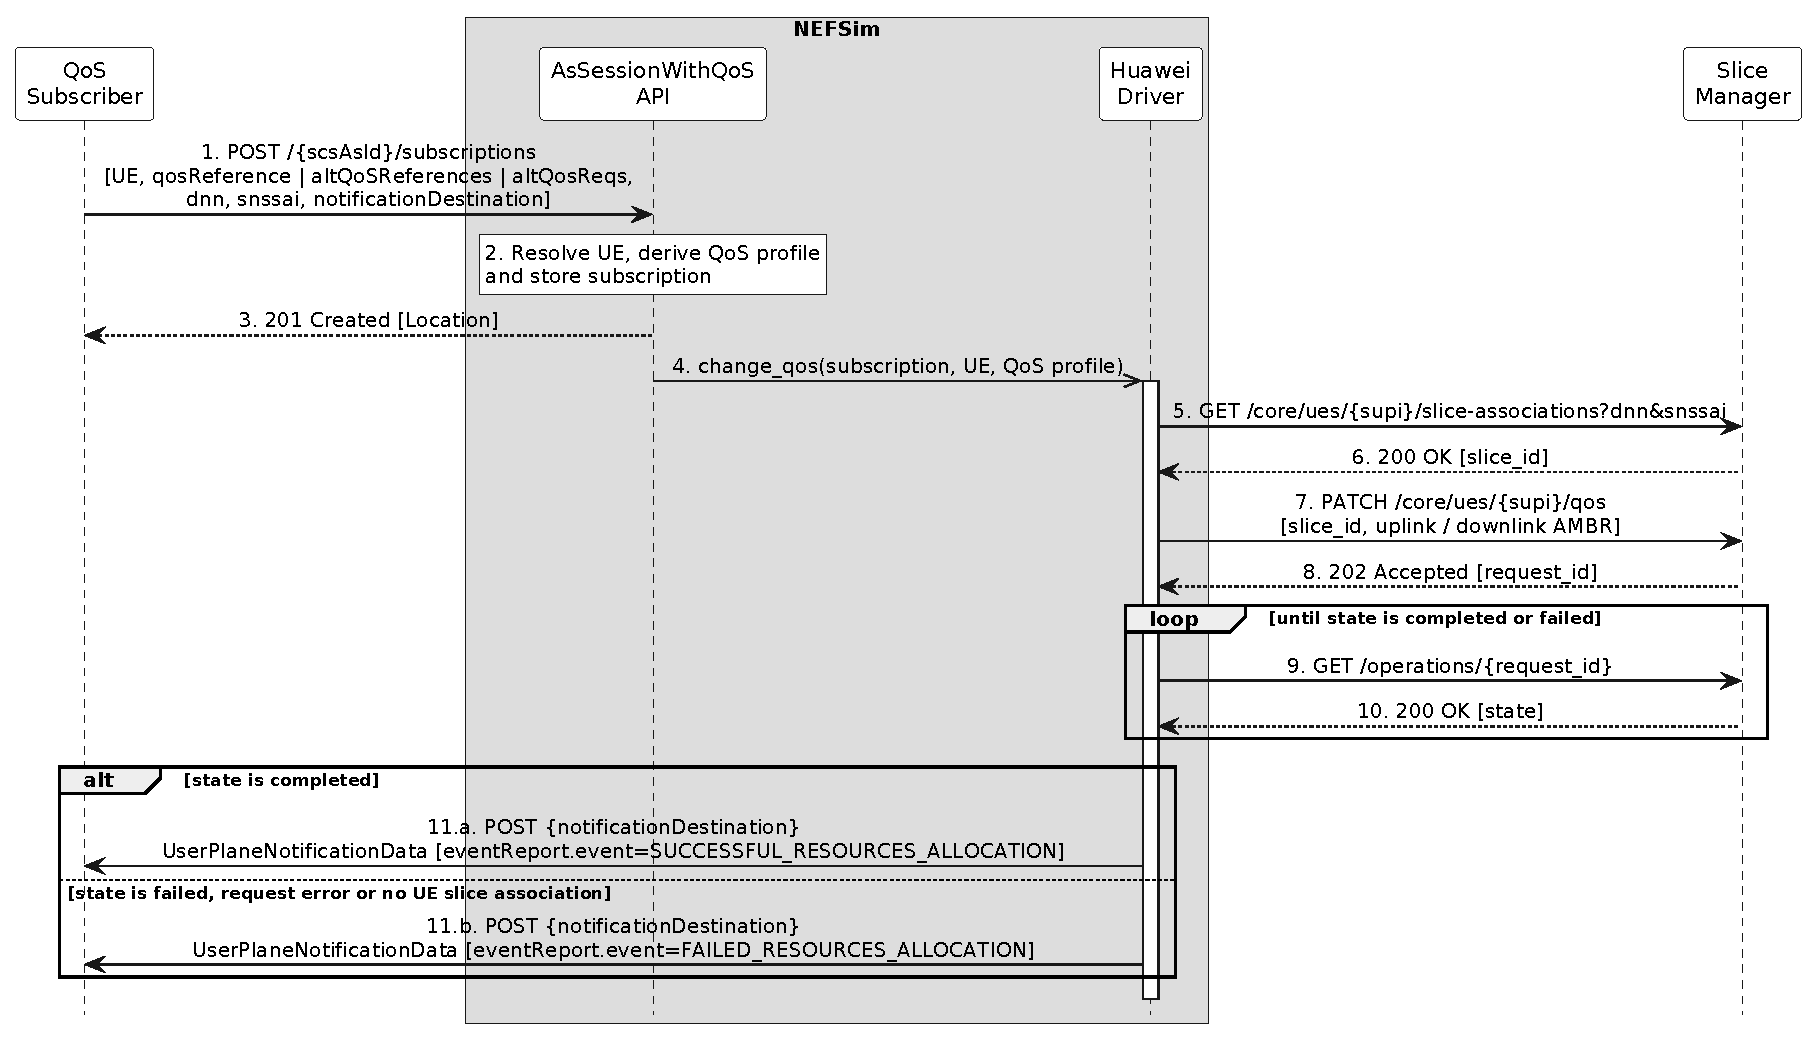
\includegraphics[width=1\linewidth]{figs/plantuml/as-session-with-qos-sequence.pdf}
    \caption{Sequence Diagram for the creation of a \acs{QoS} Subscription via the \textit{AsSessionWithQoS} \acs{API}}
    \label{fig:impl:exposure:nef:AsSessionWithQoS:sequence}
\end{figure}

The \acs{NEF}Sim \textit{AsSessionWithQoS} \acs{API} follows an optimistic, asynchronous model: the \acs{QoS} subscription is acknowledged as successfully created before the requested \acs{QoS} is actually enforced in the network (in this case, the network slice), and the subscriber is only informed of the final outcome later, through a notification.

Upon receiving a subscription request, the \acs{NEF} resolves the target \acs{UE}, derives the \acs{QoS} profile to be enforced, stores the subscription and immediately returns the reference to the subscription resource (steps 1 to 3). The \acs{QoS} profile is extracted from the subscription, either from a QoS reference (\texttt{qosReference} or \texttt{altQoSReferences}), mapped onto a set of preconfigured \acs{QoS} profiles (locally on the \acs{NEF}Sim), or from explicit \acs{QoS} requirements (\texttt{altQosReqs}), such as the uplink and downlink bit rates. The \acs{QoS} enforcement is then delegated to the Huawei driver as a background task (step 4).

Previously, subscriptions containing the \acs{DNN} and \acs{S-NSSAI} attributes were rejected by \acs{NEF}Sim. In the new implementation, these attributes are used to retrieve the slice association of the target \acs{UE} (step 5 and 6). When the subscription does not specify a \acs{DNN}, the one associated with the \acs{UE} in \acs{NEF}Sim is used instead. Once the slice association is retrieved, the driver requests the Slice Manager to update the uplink and downlink aggregate maximum bit rates of the corresponding \acs{UE}-slice association (steps 7). This way, only the \acs{QoS} of the target \acs{UE} is modified, leaving the network slice configuration untouched and ensuring that the remaining \acsp{UE} associated with the slice continue to operate under the default \acs{QoS}. Only the bitrate parameters of the \acs{QoS} profile are mapped to the Slice Manager request, as these are what's supported by the Slice Manager endpoint. If the \acs{UE} is not associated with any network slice matching the subscription, the request fails. The creation of a new network slice by the \acs{NEF} was deliberately left unsupported, since the lifecycle of network slices in the testbed, including the attachment of an \acs{UE} to a newly created slice, is managed by \acs{OSL} and the generic controller, as described in Section~\ref{chap:impl:resource_lifecycle}.

The Slice Manager accepts the request and returns an operation identifier (step 8), which the driver periodically polls until the operation state is reported as either completed or failed (steps 9 and 10). Although this approach enables asynchronous operation tracking, it is not the most efficient solution, as it requires the driver to issue repeated requests to retrieve the operation status. Ideally, this mechanism would be replaced by a callback endpoint, a common approach already adopted by multiple \acs{3GPP} and CAMARA \acsp{API}, allowing the Slice Manager to notify the driver upon completion or failure. However, since callback endpoints are not supported by the Slice Manager, periodic polling remains necessary. Finally, the \acs{NEF} notifies the subscriber with a \texttt{SUCCESSFUL\_RESOURCES\_ALLOCATION} event if the operation was completed, or a \texttt{FAILED\_RESOURCES\_ALLOCATION} event if the operation failed or no matching slice association was found (step 11).

The update and deletion of \acs{QoS} subscriptions follow a similar approach. Depending on the requested \acs{QoS} profile, these operations may trigger a revert operation to restore the \acs{UE} to the default \acs{QoS} configuration of the network slice, similarly requiring the retrieval of the \acs{UE}-slice association from the Slice Manager. As fallback, the \acs{QoS} is instead reverted to the default profile configured in \acs{NEF}Sim.

Under the CAMARA initiative, the same capability is exposed through the more user-friendly \acs{QoD} \acs{API}, which abstracts the underlying \textit{AsSessionWithQoS} procedure from network application developers. Due to this abstraction, no changes were needed to be made to the CAMARA \acs{QoD} \acs{API} already implemented at \acs{ITAv}.

\subsubsection{AnalyticsExposure \acs{API}}
\label{chap:impl:exposure:nef:AnalyticsExposure}

The \textit{AnalyticsExposure} \acs{API}, defined in \acs{3GPP}~TS~29.522~\cite{ETSI_TS_129_522_V18_11_0}, allows external consumers to retrieve analytics information generated by the \acs{5G} System, typically provided by an \acs{NWDAF}. Analytics can be obtained either through fetch requests, answered synchronously with the requested analytics data, or through a subscription-based model where the \acs{AF} can subscribe to network analytics and receive notifications periodically or when specific network conditions are met (e.g. crossing a defined threshold). In the original \acs{NEF}Sim implementation, support was limited to fetch requests for the \texttt{UE\_MOBILITY} event, which returned the simulated position of the target \acs{UE}. However, this implementation did not provide any analytics based on actual network metrics, nor did it offer analytics subscriptions, limiting its ability to expose meaningful insights into network performance and usage for network applications. In addition, since no \acs{NWDAF} is available in the 5GAIner infrastructure, there was no dedicated component from which analytics could be retrieved.

To address these limitations, a passive monitoring mechanism was developed to collect real network traffic metrics and store them in Prometheus, as described in Section~\ref{chap:impl:observability}. Specifically, it measures uplink and downlink traffic volume and throughput, categorized by source and destination \acs{IP}, \acs{MAC} address, and transport protocol. This mechanism provides an alternative source of network analytics in the absence of an \acs{NWDAF}. The \textit{AnalyticsExposure} \acs{API} implementation was then extended to retrieve these metrics from the configured Prometheus instance and expose them to external consumers, according to the \acs{3GPP}~specification~\cite{ETSI_TS_129_522_V18_11_0}.

The \textit{AnalyticsExposure} \acs{API} specification~\cite{ETSI_TS_129_522_V18_11_0} encompasses a diverse range of analytics events to support various use cases, providing insights into network performance (e.g. \texttt{NETWORK\allowbreak\_PERFORMANCE}, \texttt{DN\allowbreak\_PERFORMANCE}), resource utilization (e.g. \texttt{NS\allowbreak\_LOAD\allowbreak\_LEVEL}), and \acs{UE} information (e.g. \texttt{UE\allowbreak\_COMM}, \texttt{CONGESTION}), among others, through 14 distinct event types. An analysis of these event types and their corresponding analytics payloads was conducted to identify the most suitable option for exposing the collected metrics, i.e. uplink and downlink traffic volume and throughput. In Section~\ref{chap:proposal:exposure:camara:insights}, the \acs{GSMA} guidelines propose the \texttt{DN\allowbreak\_PERFORMANCE} event for retrieving canonical \acsp{KPI}, including packet delay budget, minimum target downlink and uplink data rates. However, upon further inspection, the corresponding response analytics schema (\texttt{DnPerfInfo}~\cite{ETSI_TS_129_522_V18_11_0}) does not distinguish between uplink and downlink traffic for any of the exposed metrics, such as bitrates, packet delay and packet loss rate. Therefore, two other analytics events were selected for the exposure of the collected metrics: \texttt{UE\_COMM} and \texttt{WLAN\_PERFORMANCE}, as summarized in Table~\ref{tab:impl:exposure:nef:AnalyticsExposure:events}.

\begin{table}[htbp]
    \centering
    \caption{Analytics events supported by the \textit{AnalyticsExposure} \acs{API}}
    \label{tab:impl:exposure:nef:AnalyticsExposure:events}
    \begin{tabularx}{\textwidth}{
        >{\raggedright\arraybackslash\hsize=0.75\hsize}X
        >{\raggedright\arraybackslash\hsize=0.75\hsize}X
        >{\raggedright\arraybackslash\hsize=1.5\hsize}X}
        \hline
        \textbf{Analytics Event} & \textbf{Reporting Scope} & \textbf{Reported Metrics} \\
        \hline
        \texttt{UE\_COMM} & Per application (\texttt{appIds}) & Mean uplink and downlink volume across the target \acsp{UE} and respective variance, flow descriptions (protocol, \acs{IP} and \acs{MAC} addresses), ratio of communicating \acsp{UE} (\acs{UE} groups only) \\
        \hline
        \texttt{WLAN\_\allowbreak PERFORMANCE} & Per \acs{UE} (\acs{GPSI}) and aggregated for all \acsp{UE} (\acs{SSID}), towards a single application server (\texttt{appServerAddrs}) & Uplink and downlink throughput, uplink, downlink and total volume, per time slot; number of target \acsp{UE} \\
        \hline
    \end{tabularx}
\end{table}

The \texttt{UE\_COMM} event characterizes the communication between the target \acsp{UE} and a set of applications, reporting the uplink and downlink traffic volume exchanged with each application. Although defined by \acs{3GPP} for \acs{WLAN} access, the \texttt{WLAN\_\allowbreak PERFORMANCE} event was adopted in this work as it allows reporting in a single payload the uplink/downlink throughput and traffic volume of each \acs{UE} over time, per time slot, according to the criteria specified by the consumer (i.e. the analytics time window and time slot duration, \texttt{temporalGranSize}).

Internally, each supported event is implemented by a dedicated handler that translates the request into a set of queries, executes them and converts the results into the corresponding \acs{3GPP} data model. The same handler serves both fetch requests and subscriptions, differing only in the delivery mechanism: analytics data are returned in the fetch response or included in an analytics event notification sent to the subscriber. As in the \textit{AsSessionWithQoS} \acs{API}, the handlers are decoupled from the metrics source through a driver interface, which provides a catalog of queries, a query builder and a query service. Two query service implementations are available: a stub service, which generates synthetic values and preserves the original simulated behavior, and a Prometheus service, which queries the Prometheus \acs{HTTP} \acs{API}. The active backend is selected at deployment time through the \acs{NEF}Sim configuration.

Figure~\ref{fig:impl:exposure:nef:AnalyticsExposure:sequence:fetch} illustrates the sequence of interactions between a consumer, the \acs{NEF} and Prometheus for the synchronous retrieval of network analytics via the \textit{AnalyticsExposure} \acs{API}.

\begin{figure}[htbp]
    \centering
    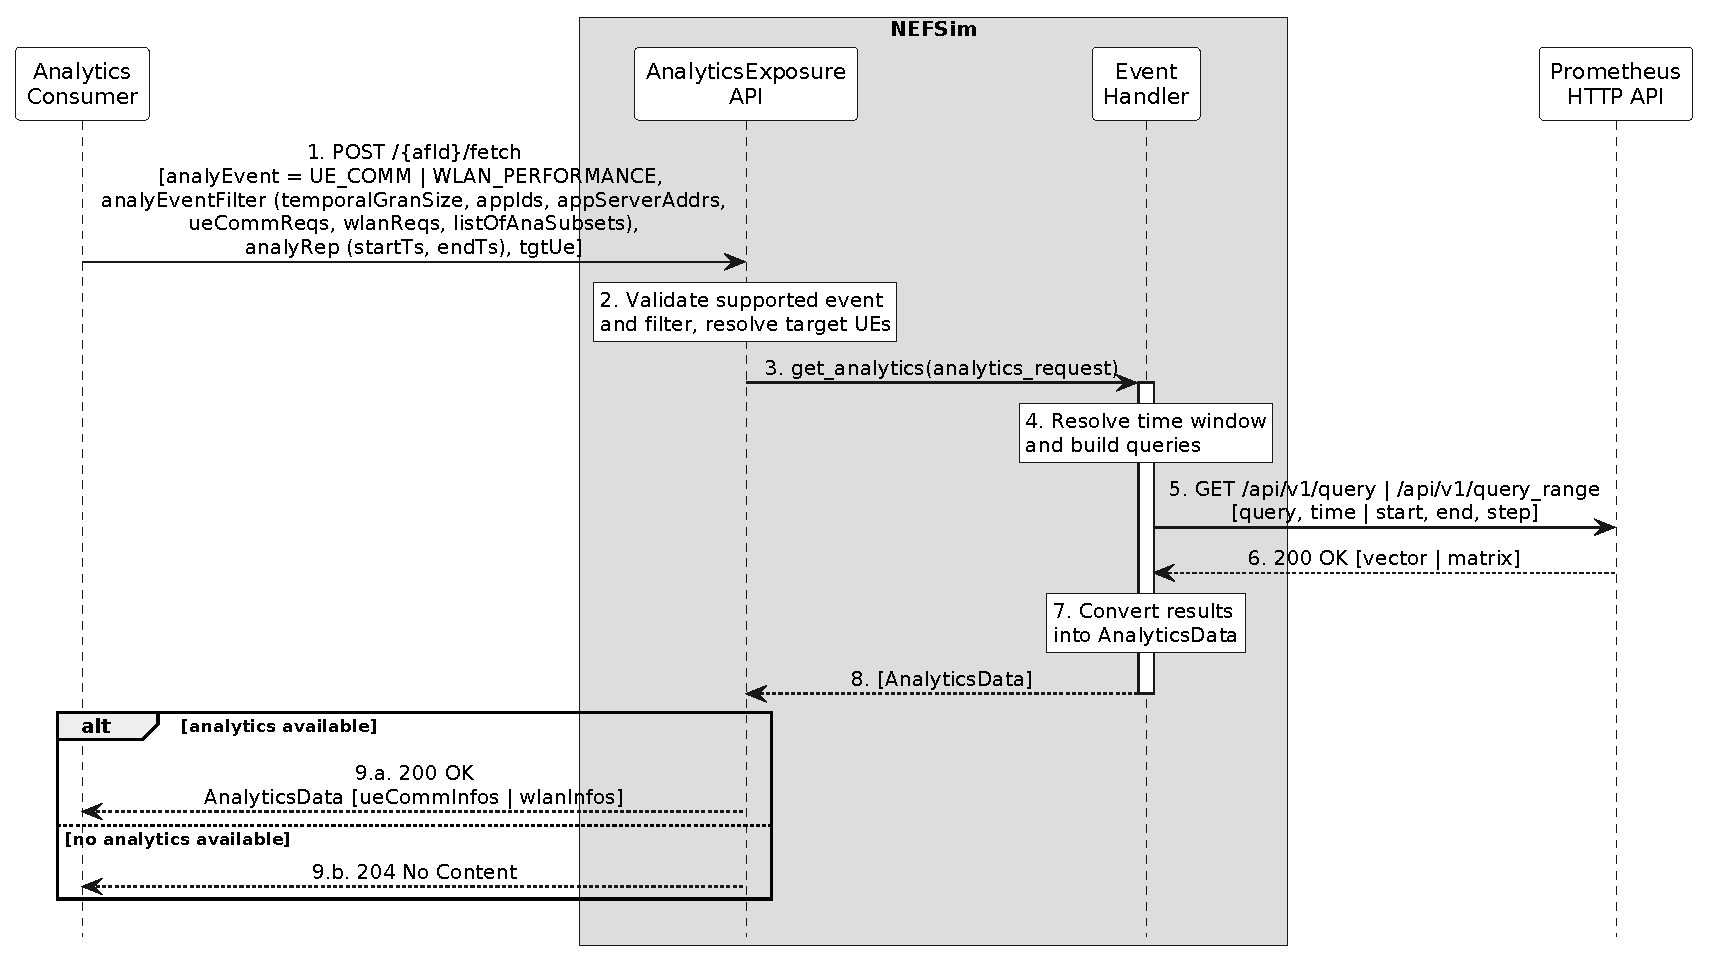
\includegraphics[width=1\linewidth]{figs/plantuml/analytics-exposure-sequence-fetch.pdf}
    \caption{Sequence Diagram for the synchronous retrieval of analytics via the \textit{AnalyticsExposure} \acs{API}}
    \label{fig:impl:exposure:nef:AnalyticsExposure:sequence:fetch}
\end{figure}

Each fetch request identifies the analytics event, the target \acsp{UE} (\texttt{tgtUe}), an optional event filter and the time window to which the analytics refer (step 1). Upon receiving it, the \acs{NEF} validates the requested event and filter, and resolves the target \acsp{UE} (step 2). Both events rely on mapping \acsp{UE} and applications to the \acs{IP} addresses observed in the monitored traffic. Target \acsp{UE} can be selected individually, through their \acs{GPSI}, collectively, through an external group identifier, or all at once, through the any- \acs{UE} indicator. For the \texttt{UE\_COMM} event, the \acs{API} must also identify the applications with which the \acsp{UE} communicate. To this end, a new \acs{NEF}Sim endpoint was introduced to register applications, associating each application identifier with its \acs{IP} and \acs{MAC} addresses. These identifiers can then be referenced in the event filter (\texttt{appIds}), restricting the analytics to the specified applications, or to all registered applications, when omitted. For the \texttt{WLAN\_PERFORMANCE} event, the application server is instead given directly in the event filter (\texttt{appServerAddrs}). The event filter may also specify the subsets of analytics to be reported (\texttt{listOfAnaSubsets}). For the \texttt{WLAN\_PERFORMANCE} event, these determine whether traffic information (\texttt{TRAFFIC\_INFO}) and the number of \acsp{UE} (\texttt{NUMBER\_OF\_UES}) are to be reported, with the remaining subsets being unsupported. The \acs{WLAN} requirements (\texttt{wlanReqs}) additionally restrict the \texttt{WLAN\_PERFORMANCE} analytics to the given (simulated) \acsp{SSID}. Both events also accept ordering criteria (specified in \texttt{ueCommReqs} and \texttt{wlanReqs}), which are applied to the reported entries.

The request is then delegated to the handler of the requested event (step 3). Before building the queries, the handler determines the time window to which the analytics refer (step 4). In synchronous requests, this window is specified through start and/or end timestamps (\texttt{startTs} and \texttt{endTs}), awalys referring to past observations, as the testbed provides no predictive model for future network conditions (e.g. an \acs{NWDAF}). According to \acs{3GPP}~\cite{ETSI_TS_129_520_V18_6_0}, temporal granularity (\texttt{temporalGranSize}) is supported for the \texttt{WLAN\_\allowbreak PERFORMANCE} event, but not for the \texttt{UE\_\allowbreak COMM} event. Hence, for this event the window is further divided into time slots according to the requested \texttt{temporalGranSize}, falling back to a configurable default. This results in a Prometheus range query with a step equal to the slot duration, each sample reporting the throughput and volume observed during the corresponding slot. In contrast, the \texttt{UE\_COMM} event is always evaluated through a single instant query covering the entire window (step 5).

The Prometheus query catalog operates over the byte counters exported by the passive monitoring component, filtered by source and destination \acs{IP} address. Uplink traffic corresponds to packets sent from the \acs{UE} towards the application, and downlink traffic in the opposite direction. Traffic volumes are computed as the increase of the counters over a given interval, and throughput as their per-second rate, converted to bits per second. All queries required by an event are combined into a single Prometheus request, with each sub-query tagged by a distinct label, reducing the number of requests and ensuring the returned samples share the same timestamps. Prometheus answers with an instant vector or a range matrix, respectively (step 6). Moreover, as Prometheus omits time series without samples in the queried window, the handlers explicitly report zeroed values in such cases, so that the absence of traffic is reported as such, rather than as missing analytics.

At the end, the handler converts the query results into the analytics data model of the requested event, i.e. the \texttt{ueCommInfos} or \texttt{wlanInfos} attributes of the \texttt{AnalyticsData} schema (steps 7 and 8), which is returned to the consumer (step 9.a). If no analytics data can be produced for the request, the \acs{NEF} instead responds with no content (step 9.b).

\plan{
    \begin{enumerate}
        \item Come back to the table (CLOSE THE TABLE)
    \end{enumerate}
}
\subsection{CAMARA \acsp{API} Integration}
\label{chap:impl:exposure:camara}

The previous subsection showed how an \acs{AF}, such as a consumer or network application, can leverage capabilities exposed through the \acs{NEF} to influence and monitor network behavior. It also highlighted the complexity involved: working with the \acs{NEF} demands a detailed understanding of \acs{3GPP} specifications and data models, particularly for the \textit{AnalyticsExposure} \acs{API}. This is a significant obstacle for application development, since vertical developers rarely have the specialized knowledge these interfaces require. In an effort to lower this barrier, the testbed offers CAMARA \acsp{API} as a simplified entry point to the same capabilities, so that developers can integrate network behavior into their applications without handling the complexity of the corresponding \acs{NEF} procedures.

The CAMARA component included in the testbed extends the GSMA Open Gateway implementation previously developed at ITAv~\cite{GSMANEFprojectIT}, a FastAPI application that implements several CAMARA \acsp{API}, including \acs{QoD}, Device Location, and Geofencing Subscriptions, providing the translation layer between these \acsp{API} and the \acs{NEF}Sim northbound interfaces. Despite this, none of the currently available \acs{API} expose insights into network conditions, similarly to what already happened in \acs{NEF}Sim before the implementation of the \textit{AnalyticsExposure} \acs{API}. Consequently, a network application accessing the network through CAMARA had no means of verifying whether the network was meeting its requirements. To close this gap, the Application Profiles and Connectivity Insights Subscriptions \acsp{API} were implemented, completing the suite of \acs{NEF} and CAMARA \acsp{API} previously established in Table~\ref{proposal:exposure:camara:nef-camara}.

\subsubsection{Application Profiles}
\label{chap:impl:exposure:camara:profiles}

In the \textit{AnalyticsExposure} \acs{API}, application network requirements are not represented by a dedicated resource. Instead, each request or subscription specifies its own analytics criteria, which, depending on the analytics event, may include thresholds for the \acs{NEF} to monitor and evaluate on behalf of the consumer. Nonetheless, for analytics events without such thresholds, as the ones considered and implemented in this dissertation, the consumer must evaluate the raw reported network metrics and compare them against the application's requirements.

The CAMARA project adopts a different approach, distinguishing between the definition of the application's network requirements and their observation and comparison. The \textit{Application Profiles}\footnote{https://camaraproject.org/application-profiles/} \acs{API} addresses the former aspect, allowing developers to specify the network conditions required by an application and store them as a structured profile. The observation and evaluation of these conditions are handled by other interfaces, namely the \textit{Connectivity Insights Subscriptions} \acs{API}, which references this profile by its identifier and assesses the observed network conditions against the defined thresholds. This separation allows the same profile to be reused across multiple subscriptions and \acsp{API}, avoiding the need to restate application requirements in each request and ensuring consistent evaluation across different monitoring services.

The \textit{Application Profiles} \acs{API} was implemented according to release r1.2\footnote{https://github.com/camaraproject/ApplicationProfiles/releases/tag/r1.2} (v0.5.0) of the CAMARA specification, supporting the four \acs{CRUD} operations: creating (\texttt{POST}), retrieving (\texttt{GET}), updating (\texttt{PATCH}), and deleting (\texttt{DELETE}) an application profile. As for the rest of the components developed throughout the dissertation, Pydantic\footnote{https://pydantic.dev/docs/validation/latest/get-started/} models were derived from the respective Open\acs{API} spec and used for data/request validation and serialization. Figure~\ref{fig:impl:exposure:camara:profiles:sequence} depicts the sequence diagram for the application profile creation operation. Similar to before, authentication and authorization branches are omitted as they'll be covered at Section~\ref{chap:impl:exposure:capif}.

\begin{figure}[htbp]
    \centering
    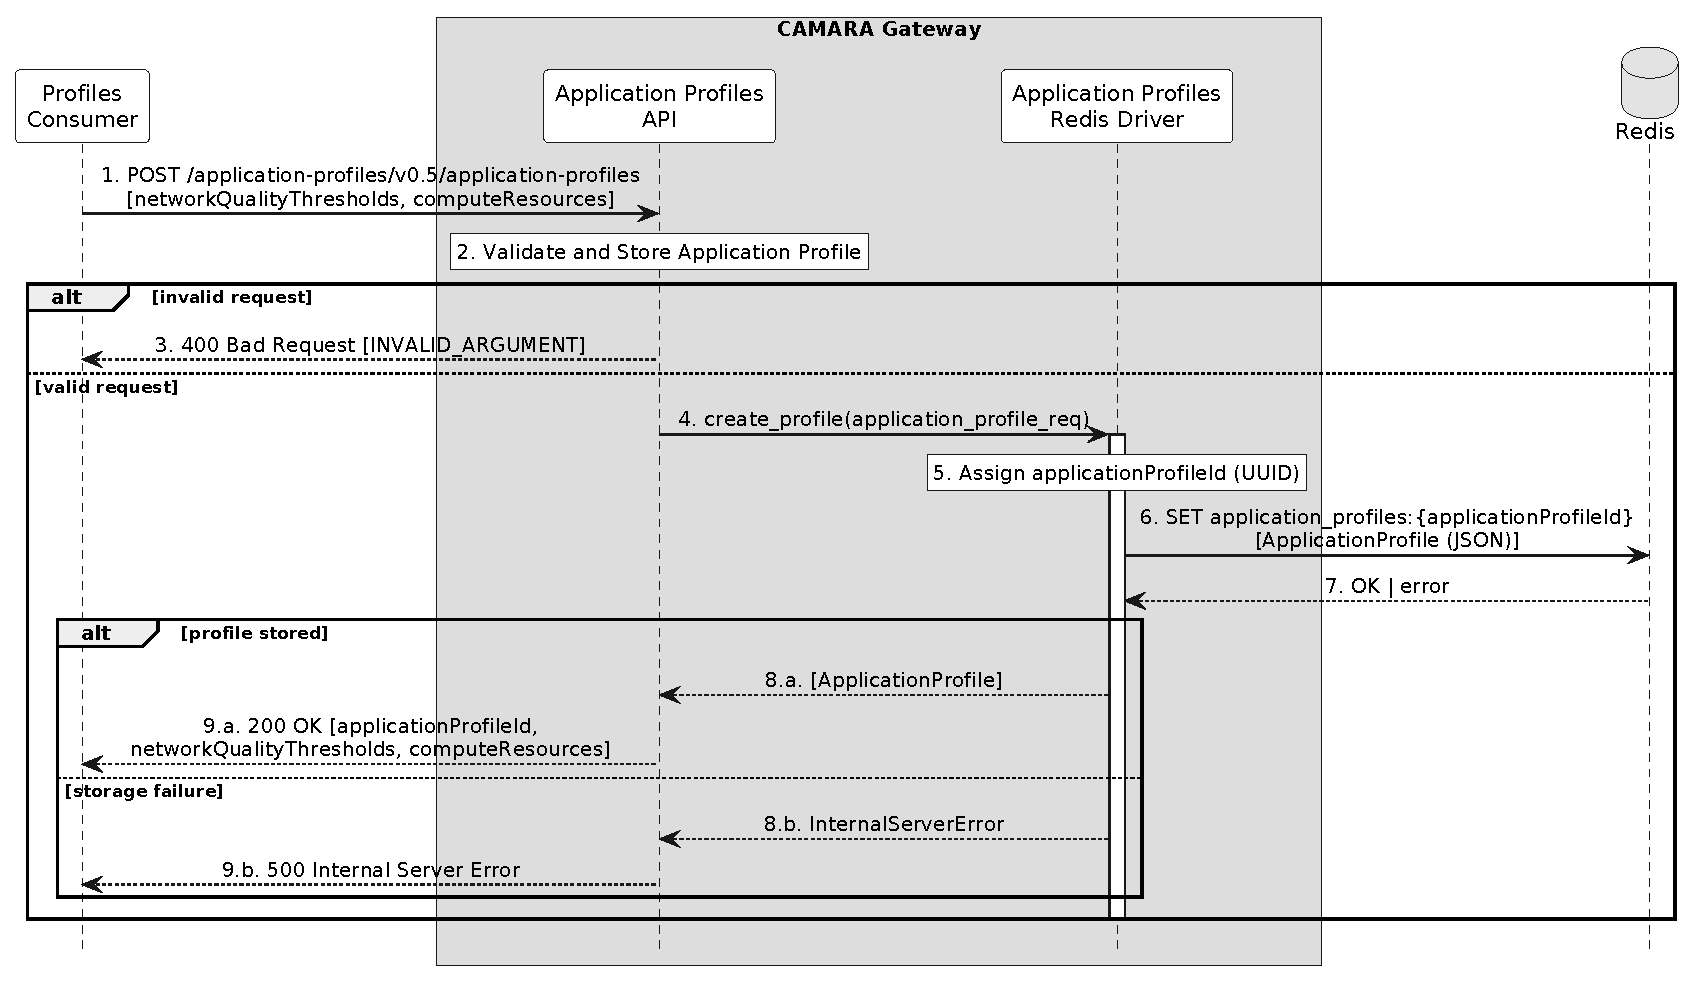
\includegraphics[width=1\linewidth]{figs/plantuml/application-profiles-sequence-create.pdf}
    \caption{Sequence Diagram for the creation of an application profile via the \textit{Application Profiles} \acs{API}}
    \label{fig:impl:exposure:camara:profiles:sequence}
\end{figure}

The interaction depicted in Figure~\ref{fig:impl:exposure:camara:profiles:sequence} is fully compliant with the \acs{NBI} realization guidelines established by \acs{GSMA}~\cite{gsmaNbiRealization} for the \textit{Application Profiles} \acs{API}, already reviewed in Section~\ref{chap:proposal:exposure:camara:profiles}. The request, declaring the network quality thresholds (and/or compute resources) required by the application, is validated and stored as an application profile. The implementation, as well as the remaining CAMARA \acsp{API} presented in this section, relies on Redis for the persistence of the created resources. This choice was first motivated by Redis being used by the already developed \acsp{API} (e.g. \acs{QoD}), which avoids introducing another persistence component. Nevertheless, it is also easily defensible from a technical stand point, as Redis closely matches the access patterns imposed by the CAMARA specifications. Every resource (e.g. an application profile, a session or a subscription) is managed exclusively through a unique identifier, which maps directly onto a key-value model. 

In this case, the profile is serialized as \acs{JSON} and stored in Redis under a key derived from a generated \acs{UUID}, i.e. the profile id, which is then returned to the client. A document-oriented database such as MongoDB would also be a viable option, but its querying capabilities would go unused, as resources are only ever accessed by identifier, making Redis the minimal option that best fits the system's needs. Finally, externalizing state to Redis keeps the exposure service stateless, allowing them to be restarted and/or horizontally scaled.

Unlike other CAMARA \acsp{API} exposed by the gateway, the \textit{Application Profiles} \acs{API} has no direct counterpart among the \acs{NEF} northbound interfaces. It is purely a management interface for application profiles, which are stored locally by the gateway without any interaction with the \acs{NEF} or the \acs{5GC}, and that are only used when referenced by other CAMARA \acsp{API}, as described next.

\subsubsection{Connectivity Insights Subscriptions}
\label{chap:impl:exposure:camara:insights}

The \textit{Connectivity Insights Subscriptions}\footnote{https://camaraproject.org/connectivity-insights-subscriptions/} \acs{API} was developed in compliance with release r3.2\footnote{https://github.com/camaraproject/ConnectivityInsights/releases/tag/r3.2} (v0.6.0), and supports the creation, retrieval, listing and deletion of analytics insights subscriptions. To provide these capabilities, the implementation interacts with the underlying \acs{NEF} to create/delete subscriptions and periodically retrieve the corresponding analytics from the configured data sources, i.e. Prometheus.

More specifically, each CAMARA subscription is realized as an \textit{AnalyticsExposure} subscription for the \texttt{WLAN\allowbreak\_PERFORMANCE} event. As discussed in Section~\ref{chap:impl:exposure:nef:AnalyticsExposure}, this event reports uplink and downlink throughput between each specified \acs{UE} and an application server. As noted earlier, this design decision departs from the \acs{GSMA} \acs{NBI} realization document~\cite{gsmaNbiRealization}, which recommended \texttt{DN\allowbreak\_PERFORMANCE}, as its associated analytics (\texttt{DnPerfInfo}) do not distinguish between uplink and downlink traffic. Table~\ref{tab:impl:exposure:camara:insights:mapping} summarizes how the fields of the CAMARA request are mapped onto the \acs{NEF} subscription.

\begin{table}[htbp]
    \centering
    \caption{\textit{Connectivity Insights Subscriptions} translation into \textit{AnalyticsExposure} subscription}
    \label{tab:impl:exposure:camara:insights:mapping}
    \begin{tabularx}{\textwidth}{@{}
        >{\RaggedRight\arraybackslash}X
        >{\RaggedRight\arraybackslash}X@{}}
        \toprule
        \textbf{\textit{Connectivity Insights Subscriptions} field} & \textbf{\textit{AnalyticsExposure} field} \\
        \midrule
        \multicolumn{2}{@{}l}{\textit{From request}} \\
        \texttt{device}                        & \texttt{tgtUe.gpsi} \\
        \texttt{applicationServer.ipv4Address} & \texttt{analyEventFilter.appServerAddrs} \\
        \texttt{subscriptionExpireTime}        & \texttt{analyRepInfo.monDur} \\
        \texttt{subscriptionMaxEvents}         & \texttt{analyRepInfo.maxReportNbr} \\
        \texttt{initialEvent}                  & \texttt{analyRepInfo.immRep} \\
        \midrule
        \multicolumn{2}{@{}l}{\textit{From configuration}} \\
        -- & \texttt{analyRepInfo.repPeriod} \\
        -- & \texttt{extraReportReq.offsetPeriod} \\
        -- & \texttt{temporalGranSize} \\
        \midrule
        \multicolumn{2}{@{}l}{\textit{Hardwired}} \\
        -- & \texttt{analyEvent} = \texttt{WLAN\_PERFORMANCE} \\
        -- & \texttt{listOfAnaSubsets} = \{\texttt{TRAFFIC\allowbreak\_INFO}, \texttt{NUMBER\allowbreak\_OF\allowbreak\_UES}\}\\
        -- & \texttt{notifMethod} = \texttt{PERIODIC} \\
        \midrule
        \multicolumn{2}{@{}l}{\textit{Replaced or not forwarded}} \\
        \texttt{sink}                          & \texttt{notifUri} = \texttt{\{gwCallback\}/\{subId\}} \\
        \texttt{applicationProfileId}          & \textit{not sent; thresholds evaluated by the gateway} \\
        \bottomrule
    \end{tabularx}
\end{table}

Each CAMARA request defines the traffic to be monitored by specifying the target device (identified by phone number or network access identifier) and the application server’s IPv4 address. It also references an application profile identifier, previously created through the \textit{Application Profiles} \acs{API}, which defines the network requirements the traffic must satisfy. Because a request accepts exactly one device, the CAMARA specification does not appear to consider monitoring multiple \acsp{UE} through a single subscription, not offering an equivalent to the \texttt{tgtUe.anyUeInd} and \texttt{tgtUe.extGroupId} parameters of the \textit{Analytics Exposure} \acs{API}. This is not specific to \textit{Connectivity Insights Subscriptions} but reflects a design decision shared across other CAMARA \acsp{API} (e.g. \acs{QoD}, Device Location) which consistently scope each request to an individual device. In this implementation, the device identifier is therefore mapped to the \acs{GPSI} of the target \acs{UE}, in the form of \texttt{msisdn-<phone number>} or \texttt{extid-<network access identifier>}. The expire time, max number of notifications and the initial event flag are also converted and forwarded on the corresponding \acs{NEF} subscription.

No other reporting parameters can be configured by the subscriber in the request. The notification method is fixed to \texttt{PERIODIC}, in accordance with the \acs{API}'s purpose of providing \textbf{periodic} connectivity insights\footnote{\url{https://raw.githubusercontent.com/camaraproject/ConnectivityInsights/r3.2/code/API_definitions/connectivity-insights-subscriptions.yaml}}. The remaining reporting parameters are therefore set at deployment time through the gateway configuration, all with a default absolute value of 5 seconds. By setting the reporting period (\texttt{repPeriod}), the analytics window (\texttt{offsetPeriod}) and the time slot duration (\texttt{temporalGranSize}) to the same value, each notification reports, in a single time slot, the uplink and downlink throughput and traffic volume observed during the interval elapsed since the previous notification. The requested analytics subsets are also explicitly set to \texttt{TRAFFIC\allowbreak\_INFO} and \texttt{NUMBER\allowbreak\_OF\allowbreak\_UES}, i.e. all metric subsets supported by \acs{NEF}Sim for the \texttt{WLAN\allowbreak\_PERFORMANCE} event.

Figure~\ref{fig:impl:exposure:camara:insights:sequence} illustrates the resulting end-to-end interaction. Starting with the creation of the analytics subscription, the request parameters are validated and the referenced application profile is retrieved from Redis, rejecting it if no such profile exists. To associate each \acs{NEF} notification with its CAMARA subscription, the subscription is assigned an \acs{UUID} that is embedded in the notification destination (\texttt{notifUri}) of the corresponding \acsp{NEF} subscription, following the translation procedure described above. The reference to the recently created \acs{NEF} subscription (\texttt{self}) is also stored in the same record for subsequent use (e.g. delete the subscription). If the \acs{NEF} rejects the request, the stored subscription is removed and the error returned to the network application (e.g. \texttt{404 Not Found} when target \acs{UE} unknown to \acs{NEF}, \texttt{500 Internal Server Error}). Notably, the thresholds of the application profile are not included in the \acs{NEF} subscription, since the \texttt{WLAN\allowbreak\_PERFORMANCE} event does not support threshold-based reporting.

\begin{figure}[htbp]
    \centering
    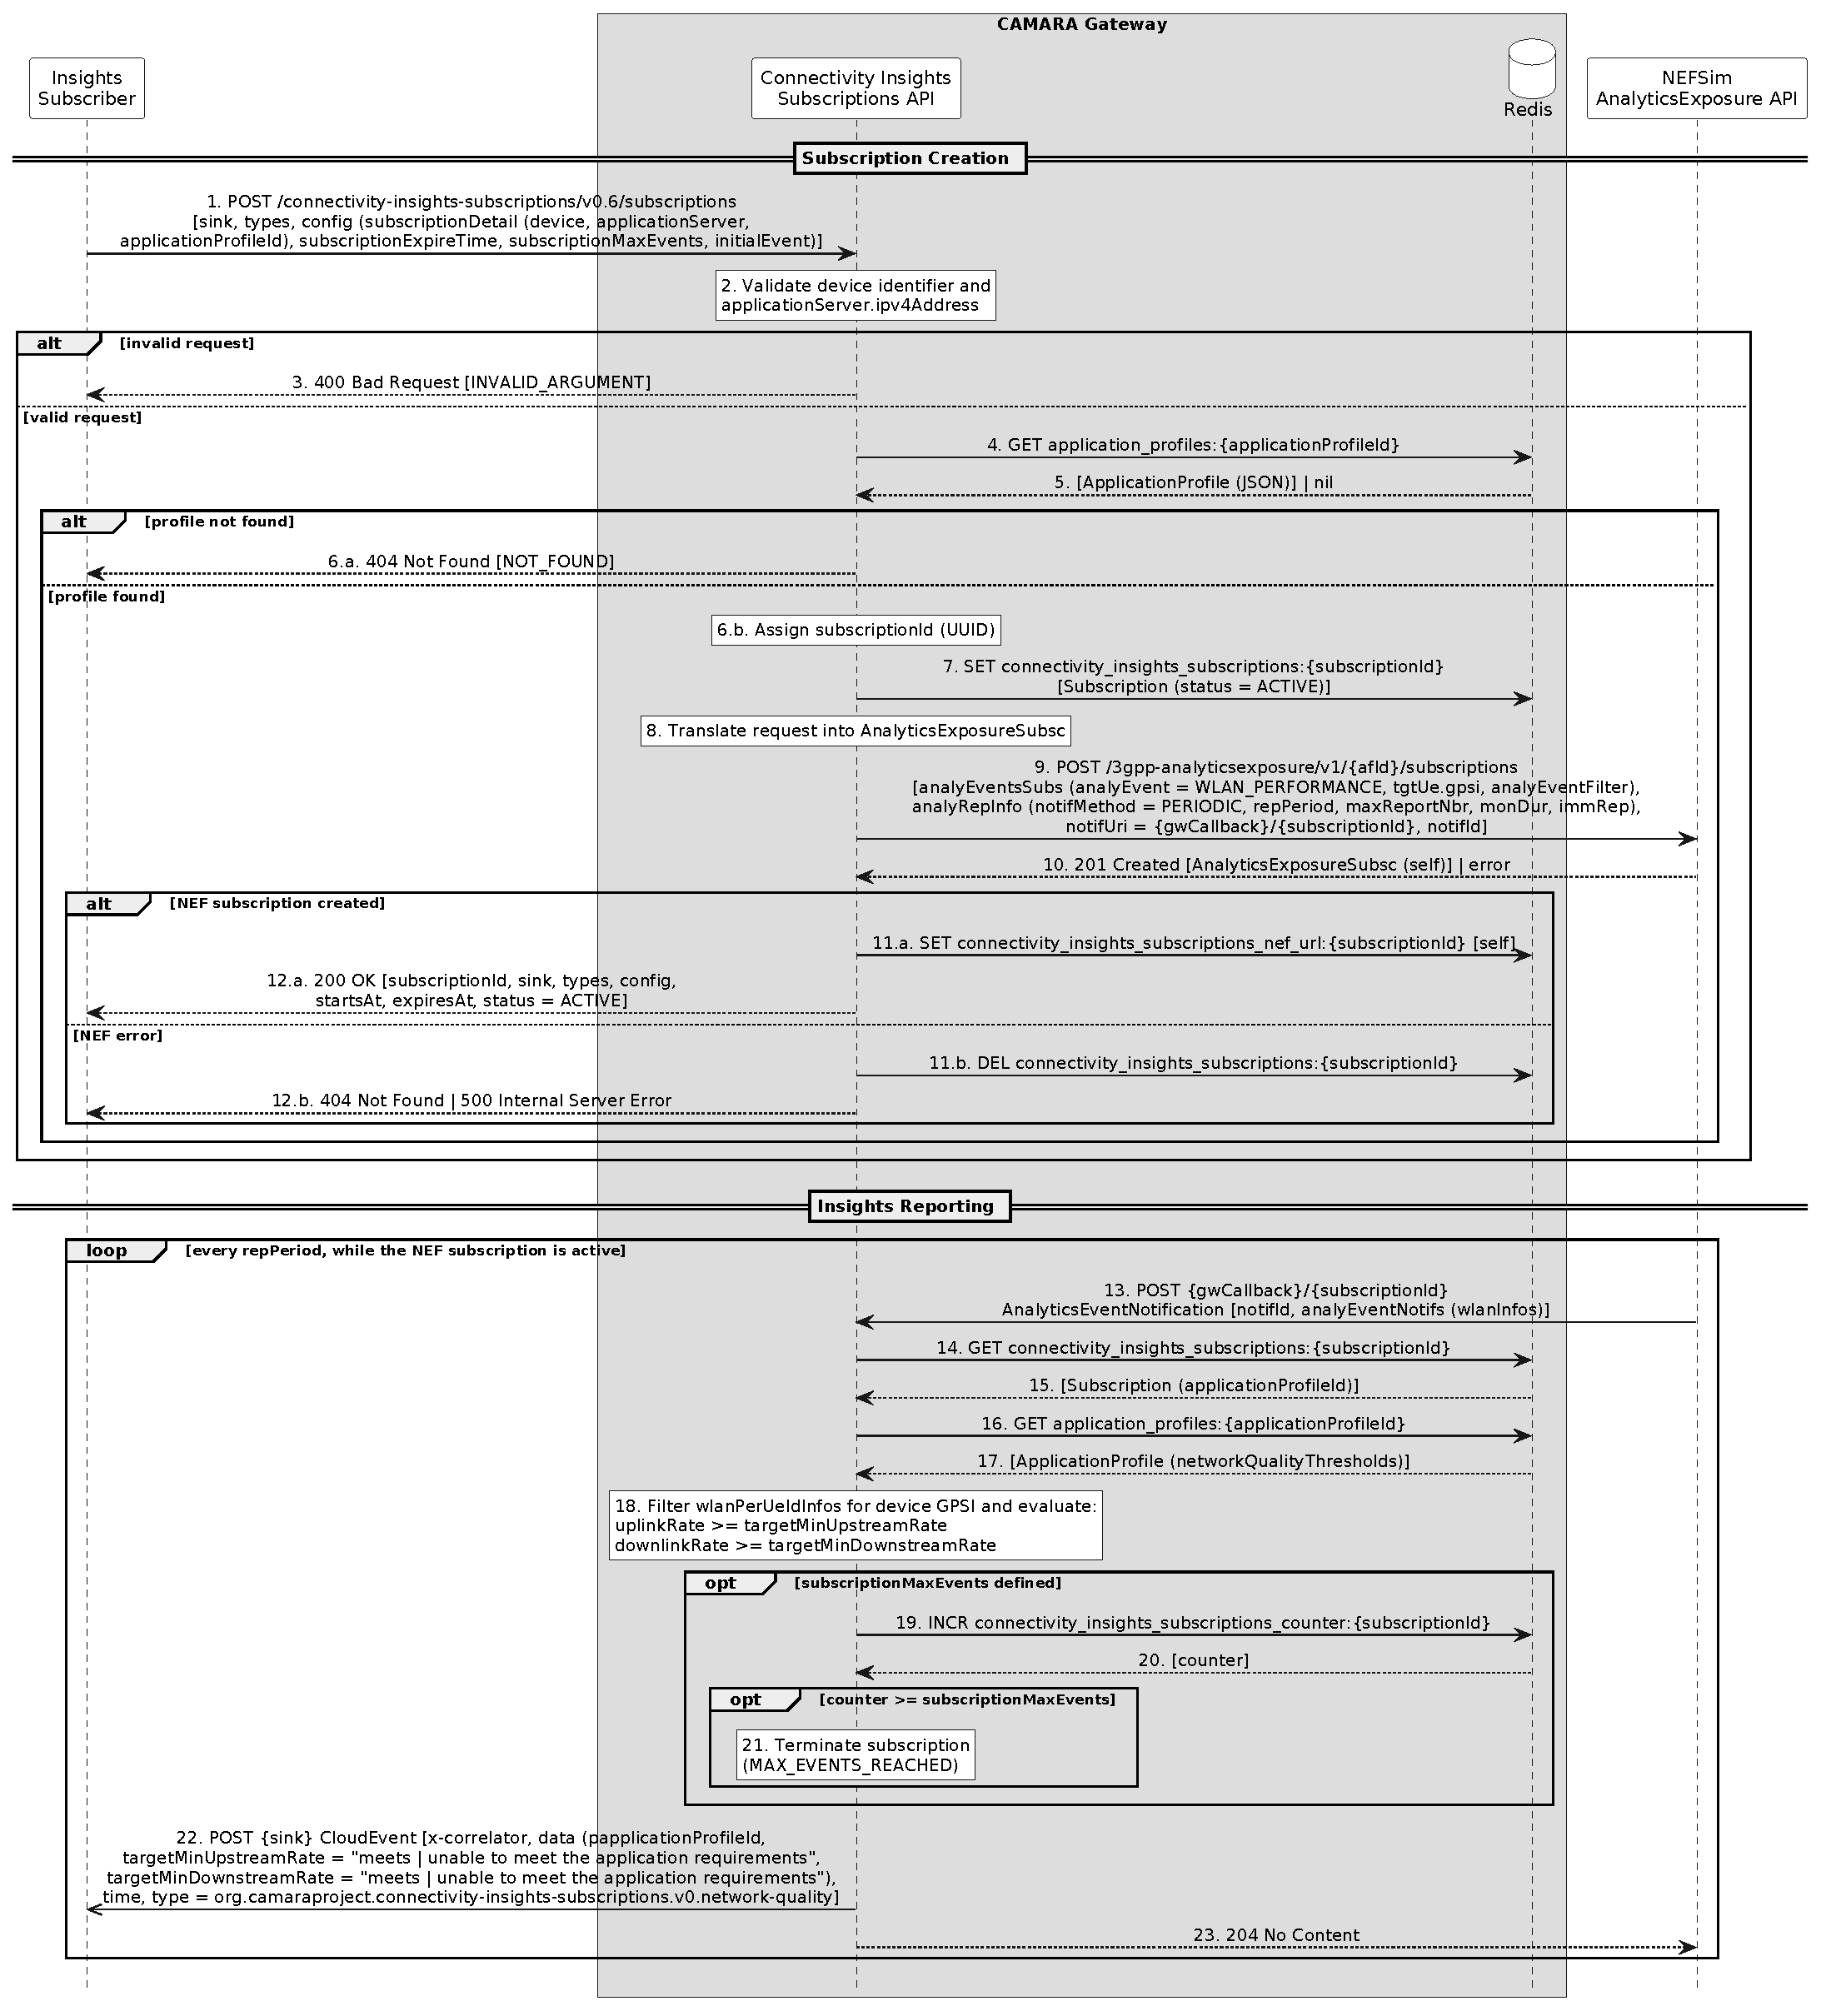
\includegraphics[width=1\linewidth]{figs/plantuml/connectivity-insights-subscription-sequence.pdf}
    \caption{Sequence Diagram for subscription creation and reporting via the \textit{Connectivity Insights Subscriptions \acs{API}}}
    \label{fig:impl:exposure:camara:insights:sequence}
\end{figure}

Instead, the \acs{NEF} periodically reports the measured uplink and downlink throughput (and volume) to the callback endpoint configured in the subscription. When a notification is received, the gateway uses the identifier provided in the callback \acs{URL} to retrieve the corresponding subscription and, subsequently the application profile. The reported uplink and downlink rates are then compared against the \texttt{targetMinUpstreamRate} and \texttt{targetMinDownstreamRate} thresholds of the profile. Each threshold is then classified as either \textit{meets the application requirements} or \textit{unable to meet the application requirements}. The resulting network quality insight, i.e. the threshold compliance status, is delivered to the original CAMARA subscriber as a background task (if max reports haven't been reached), specified in \textit{sink}. This is also characteristic of CAMARA. The notification gets relayed and may undergo some additional processing that enriches the results. The remaining network quality thresholds, i.e. packet delay budget, packet error loss rate and jitter, are not evaluated, as the testbed's passive monitoring component does not cover such metrics (Section~\ref{chap:impl:observability}).

Subscription termination reuses the subscription logic shared by other CAMARA subscription \acsp{API} of the gateway, such as Geofencing Subscriptions. A subscription is terminated when the network application deletes it, the maximum number of events is reached, its expiration time elapses, or the \acs{NEF} reports its termination. In all cases, the subscription is marked as inactive, the corresponding \acs{NEF} subscription is deleted (in the background, if it is not already), and a \texttt{subscription-ended} notification indicating the termination reason is sent to the sink.

Combined, the \textit{Application Profiles} and \textit{Connectivity Insights Subscriptions} \acsp{API} turn the raw analytics of the \textit{AnalyticsExposure} \acs{API} into application-level information. This simplifies the integration of network analytics, shielding application developers from the diversity of analytics events and payloads exposed by the underlying \acs{API}. Instead of requiring developers to interpret these analytics, manage \acs{3GPP} subscriptions, and evaluate reported metrics against application-specific thresholds, a network application declares its requirements in a profile, subscribes with the corresponding identifier, and receives a per-threshold verdict on whether the network meets them. This logic, otherwise repeated by every application relying on the \acs{NEF} directly, is thus concentrated in the exposure layer of the testbed and abstracted from the user.

\subsection{Secure \acs{API} Exposure via \acs{CAPIF}}
\label{chap:impl:exposure:capif}

Section~\ref{chap:proposal:exposure:capif} established the need for a single governance mechanism responsible for the secure publication, discovery and consumption of the testbed’s network exposure interfaces, identifying \acs{CAPIF} as the standardized framework to fulfill this role. Such a framework is essential to ensure uniform access to the network's capabilities, covering both \acs{NEF} and CAMARA \acsp{API} under a common set of procedures. To implement the standard and integrate it with the existing exposure components, the testbed adopts Open\acs{CAPIF}\footnote{\url{https://ocf.etsi.org}}~\mbox{(Release~4.0.0)}, an open source \acs{CAPIF} implementation developed by \acs{ETSI}.

Fully aligned with \mbox{3GPP~TS~29.222~Release~18}~\cite{ETSI_CAPIF_TS_129_222_V18_6_0}, Open\acs{CAPIF}\footnote{\url{https://ocf.etsi.org/documentation/latest/architecture/architecture/}} implements the \acs{CCF} \acsp{API} as a series of microservices, one per \acs{API}: Discover, Publish, Events, Invoker Management, Security, Logging, Auditing, Access Control Policy, Provider Management, Routing Info, and Open Discover, all exposed behind an Nginx reverse proxy with \acs{mTLS}. It also provides a Register service that handles user management, registering, authenticating, and managing the users that will interact with \acs{CAPIF} as Invokers or Providers. Additionally, a HashiCorp Vault\footnote{\url{https://www.hashicorp.com/en/products/vault}} instance acts as the \ac{CA}, managing and signing all \acs{CAPIF} certificates.

Among the available open source \acs{CAPIF} implementations, Open\acs{CAPIF} was selected for being standard-compliant and actively maintained by \acs{ETSI}, with regular releases tracking the evolution of the specification. It further provides a dedicated codebase for integration with the exposure ecosystem, the Open\acs{CAPIF} \acs{SDK}\footnote{\url{https://ocf.etsi.org/documentation/latest/sdk/sdk_introduction/}}, which streamlines onboarding and interaction with the \acs{CCF} for both providers, publishing their service \acsp{API}, and invokers, e.g. the network applications consuming them. Finally, its architecture aligns with the cloud-native paradigm targeted by the testbed, as all microservices are containerized and packaged as Helm charts, enabling their seamless deployment and lifecycle management alongside the remaining components of the testbed.

\subsubsection{Open\acs{CAPIF} Procedures}
\label{chap:impl:exposure:capif:procedures}

{\setlength{\emergencystretch}{3em}%
The integration of the exposure components with Open\acs{CAPIF} relies on a subset of the procedures defined in \acs{3GPP} TS~29.222~\cite{ETSI_CAPIF_TS_129_222_V18_6_0}, namely provider registration (\texttt{Register\_\allowbreak API\_\allowbreak Provider}), service \acs{API} publication (\texttt{Publish\_\allowbreak Service\_\allowbreak API}), invoker onboarding (\texttt{Onboard\_\allowbreak API\_\allowbreak Invoker}), service discovery (\texttt{Discover\_\allowbreak Service\_\allowbreak API}), access token acquisition (\texttt{Obtain\_\allowbreak Security\_\allowbreak Method} and \texttt{Obtain\_\allowbreak Authorization}) and offboarding (\texttt{Unpublish\_\allowbreak Service\_\allowbreak API}, \texttt{Deregister\_\allowbreak API\_\allowbreak Provider} and \texttt{Offboard\_\allowbreak API\_\allowbreak Invoker}). All of them are implemented through the Open\acs{CAPIF} \acs{SDK}, which translates each procedure into the corresponding requests towards the Open\acs{CAPIF} Register service and the \acs{CCF}. The \acs{NEF}Sim and CAMARA components act as \acs{API} providers, while CAMARA and the network application act as \acs{API} invokers. The following sequence diagrams detail the requests issued by the \acs{SDK} in each procedure.\par}

\bulletparagraph{\textit{Provider Registration}}

Before publishing any \acs{API}, the \acs{NEF}Sim and CAMARA components must register as \acs{API} providers in the \acs{CCF}, as illustrated in Figure~\ref{fig:impl:exposure:capif:provider-onboarding}. \acs{3GPP} TS~29.222 assumes that the provider already holds the credentials required for this registration, but leaves out of scope how they are obtained. Open\acs{CAPIF} fills this gap with its Register service, which exchanges the username and password of a previously created \acs{CAPIF} user for the \acs{CA} root certificate and a short-lived access token, later included in the registration request as its security credential. This user is not created by the provider itself, but must be created beforehand by the administrator of the Open\acs{CAPIF} instance, typically the network operator, who thereby controls which components are allowed to register in the framework.

The certificates and identifiers returned by the \acs{CCF} are persisted locally, so that a restarted instance can detect that the provider is already registered. In addition, the provider stores the certificate of the \acs{CCF} server, as its public key corresponds to the private key the \acs{CCF} uses to sign access tokens, and is therefore used by the provider to validate the tokens presented by invokers.

\begin{figure}[htbp]
    \centering
    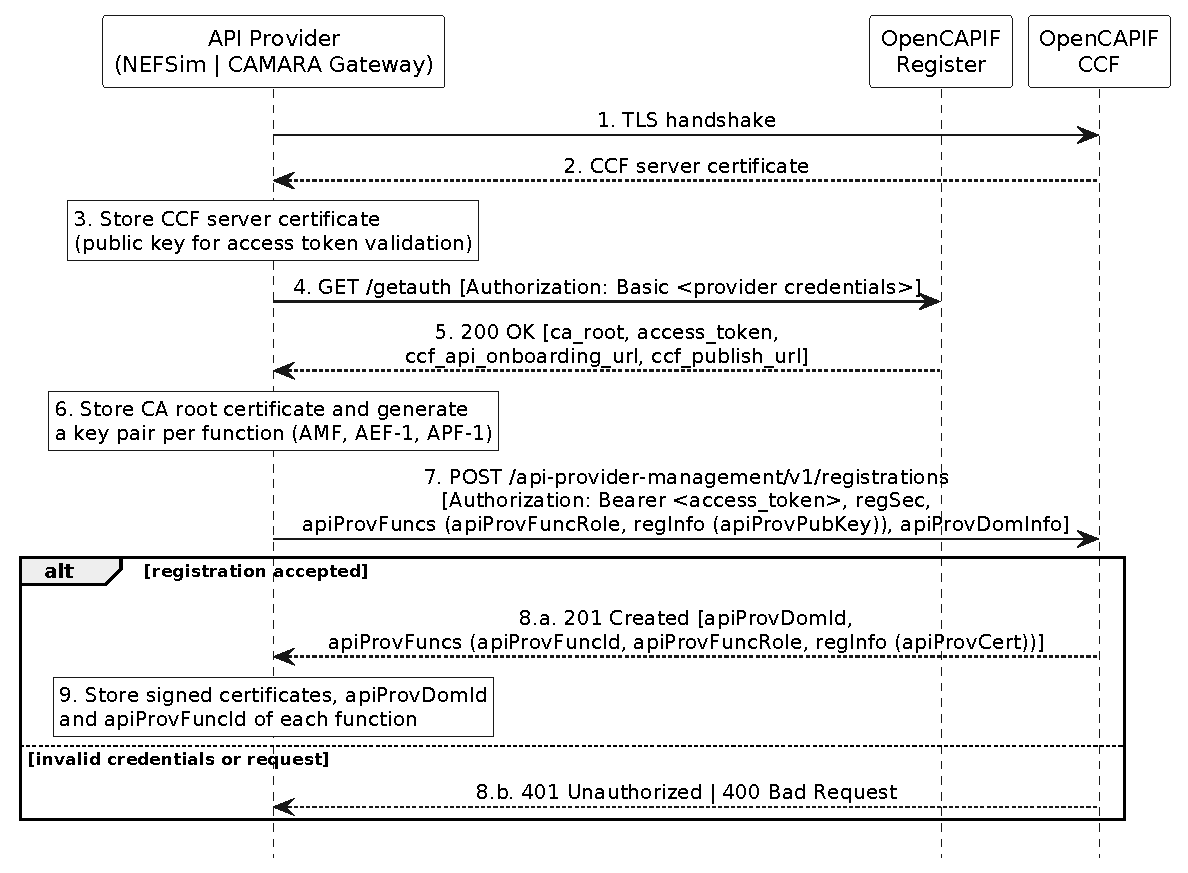
\includegraphics[width=1\linewidth]{figs/plantuml/capif/capif-provider-onboarding-sequence.pdf}
    \caption{Sequence diagram for \acs{CAPIF} provider registration}
    \label{fig:impl:exposure:capif:provider-onboarding}
\end{figure}

It should be noted that the \acs{SDK} retrieves the \acs{CCF} server certificate from the handshake of an \acs{HTTPS} connection established with certificate validation disabled, and the same applies to the request to the Register service. These are facilities provided by the Open\acs{CAPIF} \acs{SDK} to simplify development, as the trust anchors are obtained without any prior configuration. In a production deployment, the \acs{CA} root certificate and the \acs{CCF} server certificate would instead have to be provided to each component through a separate secure channel (e.g. provisioned and delivered by the network operator), since a certificate obtained over an unverified connection can be replaced by an attacker.

\bulletparagraph{\textit{Service \acs{API} Publication}}

Once registered, each provider publishes its \acsp{API} through the \acs{CAPIFAPF}, as depicted in Figure~\ref{fig:impl:exposure:capif:publication}. Instead of maintaining the service \acs{API} description manually, it is generated from the OpenAPI specification of the provider at publication time, so the published information always matches the endpoints actually served. The \acs{SDK} maps each path and \acs{HTTP} operation of the specification to a resource, named after the summary of the operation. As a result, all \acs{NEF}Sim northbound \acsp{API} are published under a single service \acs{API}, and the same applies to all CAMARA \acsp{API}.

The interface description of the \acs{CAPIFAEF} points to the public \acs{HTTPS} endpoint of the provider and declares OAuth as the only supported security method, which determines how invokers are later authorized. Since \acs{CAPIF} rejects the publication of an \acs{API} whose name is already registered, this response is interpreted by the testbed components as a previous successful publication, rather than as a failure.

\begin{figure}[htbp]
    \centering
    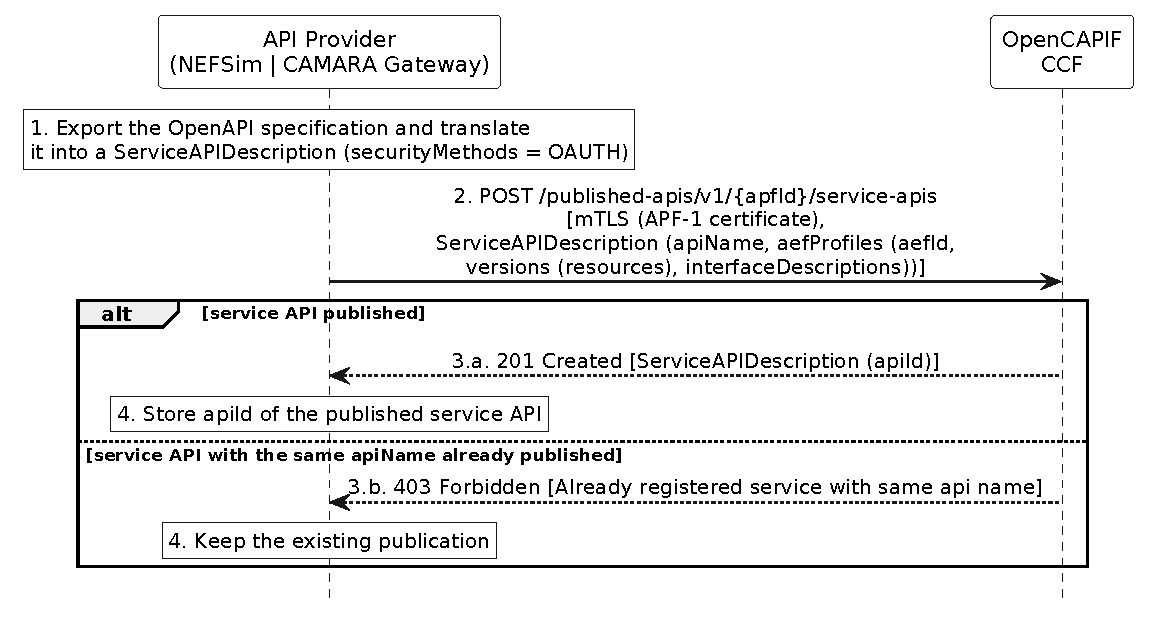
\includegraphics[width=1\linewidth]{figs/plantuml/capif/capif-api-publication-sequence.pdf}
    \caption{Sequence diagram for \acs{CAPIF} service \acs{API} publication}
    \label{fig:impl:exposure:capif:publication}
\end{figure}

\bulletparagraph{\textit{Invoker Onboarding}}

Invoker onboarding, shown in Figure~\ref{fig:impl:exposure:capif:invoker-onboarding}, follows the same pattern as provider registration, relying on the Register service to obtain the onboarding credentials. It is performed by CAMARA, as an invoker of the \acs{NEF}Sim \acsp{API}, and by the network application, as an invoker of both the \acs{NEF}Sim and CAMARA \acsp{API}, each with its own \acs{CAPIF} user.

The invoker identifier returned by the \acs{CCF} is the key of all subsequent invoker procedures, from discovery to token issuance, and is persisted together with the certificate. This way, a restarted invoker reuses its existing identity, which is confirmed by a successful discovery request, instead of onboarding as a new invoker.

\begin{figure}[htbp]
    \centering
    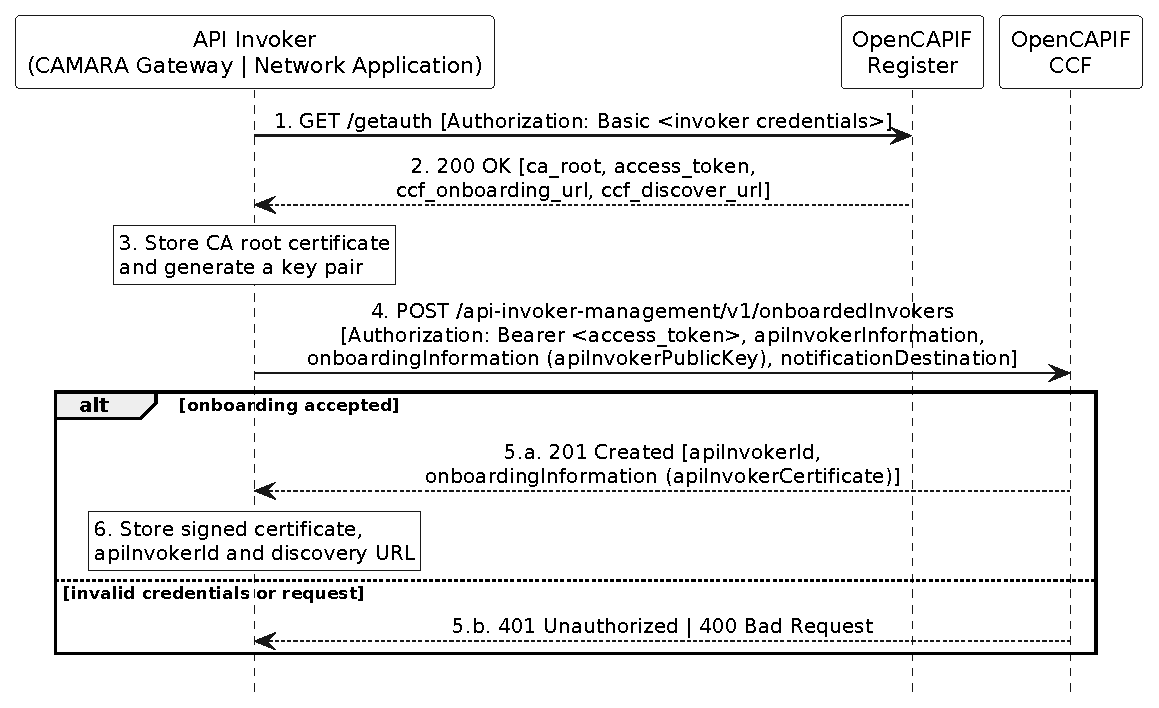
\includegraphics[width=1\linewidth]{figs/plantuml/capif/capif-invoker-onboarding-sequence.pdf}
    \caption{Sequence diagram for \acs{CAPIF} invoker onboarding}
    \label{fig:impl:exposure:capif:invoker-onboarding}
\end{figure}

\bulletparagraph{\textit{Service Discovery}}

Through service discovery, illustrated in Figure~\ref{fig:impl:exposure:capif:discovery}, invokers learn which \acsp{API} are available and where they are exposed, without any endpoint being configured in advance. The testbed components apply no discovery filters, retrieving every service \acs{API} visible to the invoker in a single request. Consequently, the network application receives the descriptions published by both providers and selects the appropriate one by its \acs{API} name, while CAMARA uses the description published by the \acs{NEF}Sim. Discovery is thus performed once at startup, with the retrieved information stored locally and reused for every subsequent \acs{API} invocation.

\begin{figure}[htbp]
    \centering
    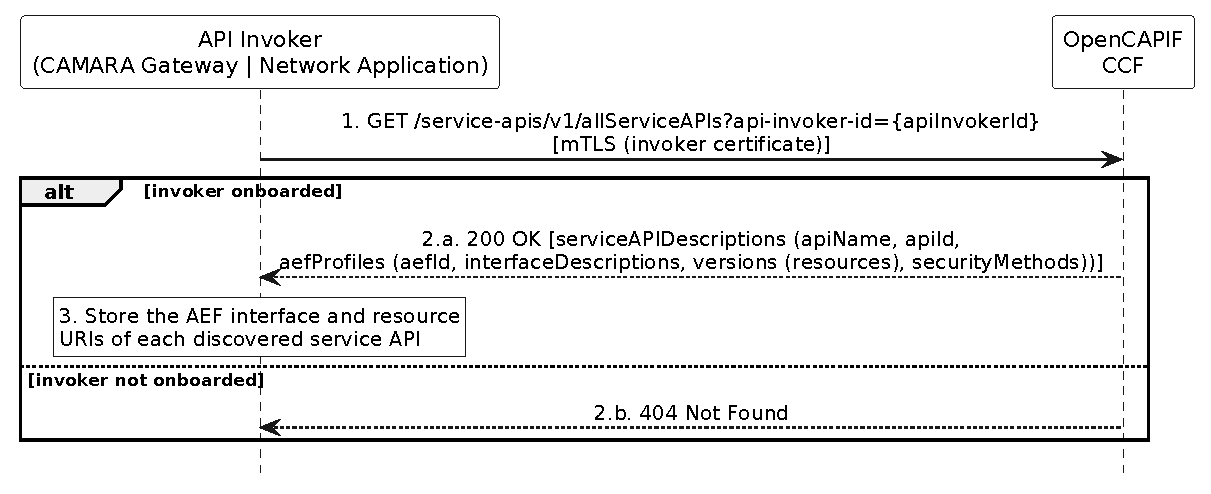
\includegraphics[width=1\linewidth]{figs/plantuml/capif/capif-service-discovery-sequence.pdf}
    \caption{Sequence diagram for \acs{CAPIF} service discovery}
    \label{fig:impl:exposure:capif:discovery}
\end{figure}

\bulletparagraph{\textit{Access Token Acquisition}}

Access to the discovered \acsp{API} is governed by the Security \acs{API} of the \acs{CCF}, as depicted in Figure~\ref{fig:impl:exposure:capif:access}. The invoker must first hold a security context, i.e. a record in the \acs{CCF} associating it with the \acsp{API} it intends to consume and the security method to be applied to each, which in the testbed is always OAuth, as declared by the providers. Based on this context, the invoker obtains an access token through the OAuth~2.0 client credentials grant.

As the requested scope lists every \acs{CAPIFAEF} and \acs{API} pair in the security context, a single \acs{JWT} authorizes the network application towards both the \acs{NEF}Sim and CAMARA. Authentication and authorization are therefore split between two mechanisms: the invoker certificate, verified through \acs{mTLS}, proves the identity of the invoker, while the token proves that the \acs{CCF} has authorized it. Being signed by the \acs{CCF}, the token is validated locally by the \acs{CAPIFAEF} with the \acs{CCF} public key, which keeps the \acs{CCF} out of the path of every \acs{API} invocation.

\begin{figure}[htbp]
    \centering
    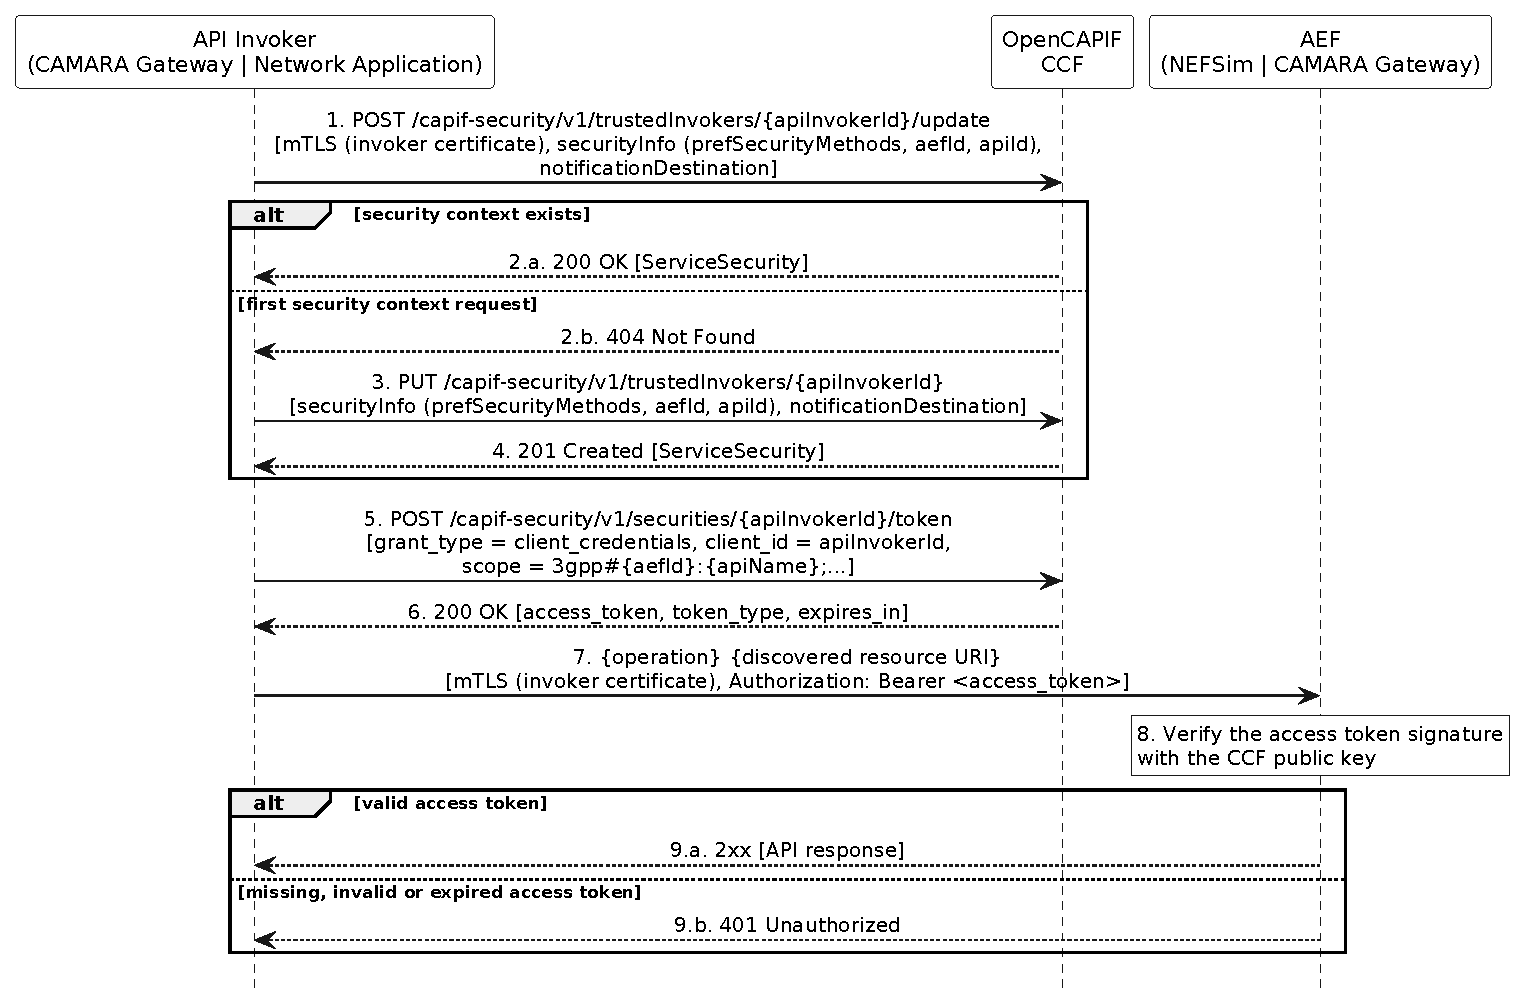
\includegraphics[width=1\linewidth]{figs/plantuml/capif/capif-api-access-sequence.pdf}
    \caption{Sequence diagram for \acs{CAPIF} access token acquisition and \acs{API} invocation}
    \label{fig:impl:exposure:capif:access}
\end{figure}

Similarly to the retrieval of certificates, the creation of the security context is a facility of the Open\acs{CAPIF} \acs{SDK}. The \acs{SDK} builds the security context on the invoker side, automatically covering every discovered \acs{API} and filling the authentication and authorization information with placeholder values. In a production deployment, the \acsp{API} an invoker is authorized to consume would not be determined by the invoker itself, but by the access policies defined in the \acs{CCF} by the providers and the network operator.

\bulletparagraph{\textit{Offboarding}}

The offboarding procedures, shown in Figure~\ref{fig:impl:exposure:capif:offboarding}, keep the state of the \acs{CCF} consistent with the components actually deployed. Without them, invokers would keep discovering \acsp{API} whose providers are no longer running, and the identities of removed components would accumulate in the \acs{CCF}. Each step is authenticated by the function responsible for the corresponding resource: the service \acs{API} is unpublished with the \acs{CAPIFAPF} certificate, and the provider registration is deleted with the \acs{CAPIFAMF} certificate, while invokers delete their onboarding resource with their own certificate. The locally persisted certificates and identifiers are removed as well, meaning that an offboarded component must go through registration or onboarding again at its next startup, under a new identity.

\begin{figure}[htbp]
    \centering
    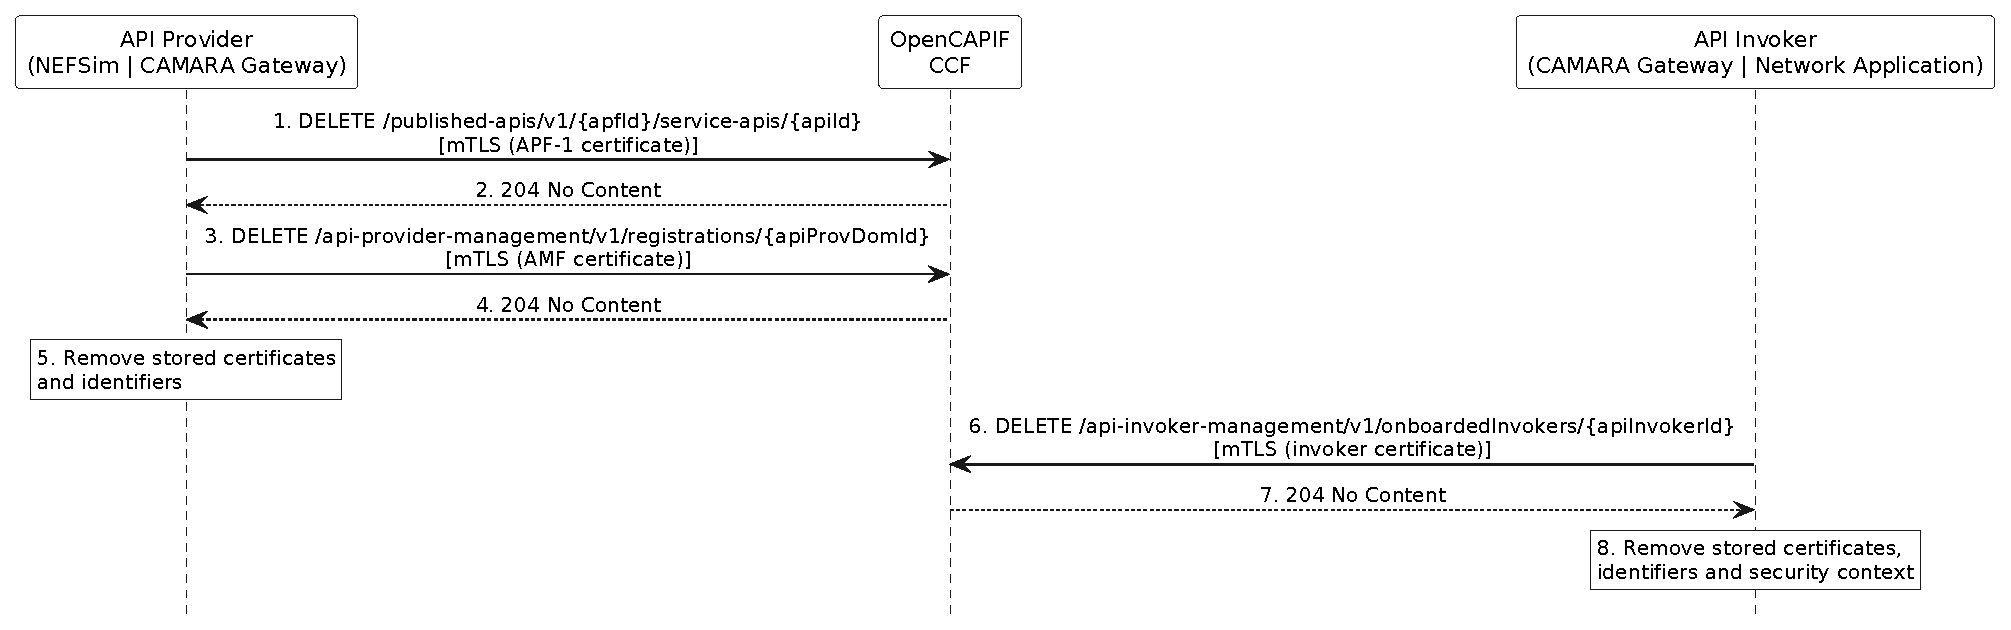
\includegraphics[width=1\linewidth]{figs/plantuml/capif/capif-offboarding-sequence.pdf}
    \caption{Sequence diagram for \acs{CAPIF} provider and invoker offboarding}
    \label{fig:impl:exposure:capif:offboarding}
\end{figure}

\subsubsection{Open\acs{CAPIF} Integration}
\label{chap:impl:exposure:capif:opencapif}

Integrating Open\acs{CAPIF} into the testbed required realizing these procedures on both sides of the exposure chain, for both providers (i.e. \acs{NEF} and CAMARA) and the invokers (i.e. CAMARA and the network application). For the \acs{NEF}, this was expected to be more straightforward, as its built-in \acs{CAPIF} support was a key reason for selecting the \acs{NEF}Sim implementation in the first place. More concretely, the original upstream version of the emulator\footnote{\url{https://github.com/EVOLVED-5G/NEF_emulator}} relied on the EVOLVED-5G \acs{SDK}\footnote{\url{https://github.com/EVOLVED-5G/SDK-CLI/blob/master/evolved5g/sdk.py}}, which provides dedicated classes for provider onboarding and \acs{API} publication, invoker onboarding, invocation logging and auditing, service discovery, and OAuth-based authorization. From these, the emulator utilized the provider classes to onboard and publish the MonitoringEvent and AsSessionWithQoS \acsp{API}, logging each invocation to \acs{CAPIF}. Incoming requests were authorized by verifying the signature of the \acs{CAPIF}-issued access tokens (i.e. \acsp{JWT}) with the \acs{CAPIF} server's public key.

This implementation was validated with older Open\acs{CAPIF} versions. However, a closer assessment of the implementation revealed that the \acs{SDK}'s integration had not kept pace with subsequent releases of the framework, resulting in erroneous and inconsistent behavior, for the most recent Open\acs{CAPIF} releases. Thus, this dissertation uses the aforementioned Open\acs{CAPIF}~\acs{SDK}\footnote{\url{https://pypi.org/project/opencapif-sdk/}}, a Python package maintained alongside the \acs{CCF} within the \acs{ETSI}~Open\acs{CAPIF} project and kept compatible with its public releases, to implement provider and invoker procedures in the \acs{NEF}Sim, CAMARA and network application components. This also simplifies the integration process as the testbed grows, since new exposure interfaces, whether \acs{NEF}, CAMARA or even proprietary \acsp{API}, can reuse the same \acs{SDK} functionality instead of reimplementing the \acs{CAPIF} procedures. The same applies to any new network applications that third parties may wish to develop, provided they are built within the Python ecosystem.

Since both the \acs{NEF}Sim and CAMARA interfaces are implemented with Fast\acs{API}\footnote{\url{https://fastapi.tiangolo.com}}, a Python web framework for building \acsp{API}, the Open\acs{CAPIF} \acs{SDK} is integrated through two mechanisms provided by the framework, each covering a distinct stage of the procedures described earlier. This approach also ensures the implementation of the \acs{CAPIF} flows remains independent of the testbed deployment environment, supporting development and operation outside the testbed (e.g. in non-Kubernetes environments, using Docker Compose, or in local deployments with a separate \acs{CAPIF} instance), in line with the goal of the corresponding open source repositories. 

Fast\acs{API}'s lifespan events provide a mechanism for defining custom code to be executed during application startup and shutdown, allowing \acs{CAPIF} procedures to be tied to the application lifecycle. At startup, the \acs{NEF}Sim onboards as an \acs{API} provider and publishes its \acsp{API} to the \acs{CCF}, using a \acs{CAPIF} user already created beforehand (an additional step was included in the Open\acs{CAPIF} deployment scripts to create a user for the \acs{NEF}, CAMARA and a third party application). This operation is idempotent, ensuring the \acs{NEF} and its \acsp{API} are registered exactly once, across restarts or multiple instances (e.g. Kubernetes replicas). Symmetrically, at shutdown, the offboarding procedure is executed, automatically unpublishing the corresponding \acsp{API}. However, to prevent the application from deregistering the provider and unpublishing its \acsp{API}, in the case of a multi-replica setup, the offboarding procedure at shutdown is disabled by default.

The CAMARA component extends this behavior, additionally invoking the Open\acs{CAPIF} \acs{SDK} to perform the \acs{API} invoker procedures. This includes onboarding as an invoker and discovering all available \acsp{API} associated with its invoker id at startup. Invoker offboarding at shutdown follows the same rule, being disabled by default.

The \acsp{URL} of the discovered \acsp{API} are subsequently resolved from the information obtained during onboarding and discovery, without additional \acs{CAPIF} calls. As illustrated in Code Block~\ref{code:impl:exposure:capif:discover}, the \texttt{discover\_nef\_url} function identifies the appropriate endpoint based on the \acs{API} name, resource name, and \acs{HTTP} operation. A fallback \acs{URL} is provided for when \acs{NEF}'s \acs{CAPIF} authentication and authorization is disabled. The network application also adopts a similar invoker logic. All three implementations rely on separate \texttt{capif\_invoker} and \texttt{capif\_provider} singletons and helper functions, each built around the Open\acs{CAPIF} \acs{SDK} objects. The complete source code of the \acs{CAPIF} integration for the \acs{NEF}Sim\footnote{\url{https://github.com/Testbed-TNEI/NEF_emulator/tree/main/backend/app/app/capif}}, CAMARA\footnote{\url{https://github.com/Testbed-TNEI/gsma-open-gw-apis/tree/main/gateway/app/capif}} and network application\footnote{\url{https://github.com/Testbed-TNEI/VehicleDetectionPoC/tree/main/app/app/capif}} components is also available.


\begin{listing}[htbp]
\begin{minted}{python}
res = await self.httpx_client.post(
    discover_nef_url(
        nef_settings=self.nef_settings,
        fallback="/3gpp-as-session-with-qos/v1/{scsAsId}/subscriptions",
        resource_name="Create Subscription",
        api_name_filter="as-session-with-qos",
        operation="POST",
    ).format(scsAsId=self.af_id),
    content=payload.model_dump_json(exclude_unset=True),
    headers={"Content-Type": "application/json"},
)
\end{minted}
\caption{CAMARA invocation of \acs{NEF} \acs{API} using \acs{CAPIF} discovery results}
\label{code:impl:exposure:capif:discover}
\end{listing}

The remaining \acs{CAPIF} procedures occur on a per-request basis and are therefore handled by components that intercept each request, on the provider side for incoming requests and on the invoker side for outgoing ones.

On the provider side, access token validation is implemented as a Fast\acs{API} dependency, i.e. a reusable function the framework resolves and executes before each path operation. This dependency is responsible for extracting the bearer token from the \texttt{Authorization} header and validating it against the \acs{CCF} public key obtained during provider onboarding. Requests with missing, expired or out-of-scope tokens are rejected by the dependency before the path operation is executed, returning \texttt{401 Unauthorized} when the token is absent, malformed or expired, and \texttt{403 Forbidden} when a valid token does not grant access to the requested \acs{API}. By concentrating token validation in a single dependency, the route handlers of \acs{NEF}Sim and of the CAMARA \acsp{API} remain agnostic to the \acs{CAPIF} integration, allowing developers to focus solely on each \acs{API}'s functional logic, with the same dependency being reused across all \acs{API}.

On the invoker side, the CAMARA (and the \acs{PoC}) consume the \acs{NEF}Sim (and CAMARA) \acsp{API} through an \texttt{httpx} client configured with a custom authentication class, which preemptively verifies the expiry of the current access token and attaches it to the request as a bearer token. If the token is deemed expired or the \acs{NEF} responds with \texttt{401 Unauthorized}, possible in near-expiry scenarios, the class requests a new token from the \acs{CCF}, retrying the invoker request at most once. This way, token acquisition and renewal are also transparent to the code issuing the requests.

Lastly, to establish secure communication between the two roles, the provider enforces \acs{mTLS}, which requires both the client (invoker) and the server (provider) to verify each other's identity using X.509 digital certificates before data exchange begins. This is achieved through an Nginx reverse proxy, one placed in front of each \acs{CAPIFAEF}, i.e. \acs{NEF} and CAMARA, as depicted in Code Block~\ref{code:impl:exposure:capif:nginx}. The configuration relies on three certificate-related directives to establish the \acs{HTTPS} connection: \texttt{ssl\_certificate} and \texttt{ssl\_certificate\_key} hold the \acs{CAPIFAEF}’s own certificate and private key, presented to the invoker during the handshake to prove the server's identity, while \texttt{ssl\_client\_certificate} contains the root certificate of the \acs{CCF}, acting as the \ac{CA}, against which the certificates presented by invokers are validated. Plain \acs{HTTP} requests are automatically redirected to their \acs{HTTPS} counterparts, with requests presenting an invalid client certificate being rejected with \texttt{403 Forbidden}, rather than Nginx's default \texttt{400 Bad Request}. The \texttt{proxy\_pass} directive then forwards the incoming requests to the corresponding backend service, including the \acs{URL}-encoded client certificate in the \texttt{X-SSL-Client-Cert} header.

\begin{listing}[htbp]
\begin{minted}{nginx}
server {
    listen 80;
    server_name _;
    return 301 https://$host:443$request_uri;
}

server {
    listen 443 ssl;

    ssl_certificate         /etc/nginx/provider-certs/provider/aef-1.crt;
    ssl_certificate_key     /etc/nginx/provider-certs/provider/AEF-1_private_key.key;
    ssl_client_certificate  /etc/nginx/provider-certs/provider/ca.crt;
    ssl_verify_client       optional;

    location / {
        if ($ssl_client_verify != SUCCESS) {
            return 403;
        }
        proxy_set_header X-SSL-Client-Cert $ssl_client_escaped_cert;
        proxy_pass http://backend:80/;
    }
}
\end{minted}
\caption{Nginx \acs{mTLS} Configuration for \acs{CAPIFAEF} reverse proxy}
\label{code:impl:exposure:capif:nginx}
\end{listing}

All these certificates required for mutual authentication, for both roles, are generated and provided by Open\acs{CAPIF} as part of the onboarding process. This ensures that only invokers holding certificates issued by the trusted \acs{CAPIF} instance can establish a secure connection with the provider. It also prevents unauthorized entities from impersonating legitimate invokers or providers, that are actually registered with the \acs{CCF}, mitigating the risk of man-in-the-middle attacks.

Integrating \acs{CAPIF} and \acs{mTLS} into the authentication and authorization process also required changing the deployment \acs{IaC} manifests, including creating the Nginx Docker image~\footnote{\url{https://github.com/Testbed-TNEI/NEF_emulator/blob/main/nginx/Dockerfile.nginx}} and adapting the \acs{NEF}Sim docker compose~\footnote{\url{https://github.com/Testbed-TNEI/NEF_emulator/blob/main/docker-compose.yml}}, and the Helm charts of the \acs{NEF}Sim~\footnote{\url{https://github.com/Testbed-TNEI/NEF_emulator/tree/main/helm-chart}}, CAMARA\footnote{\url{https://github.com/Testbed-TNEI/gsma-open-gw-apis/tree/main/charts/gateway}} and network application\footnote{\url{https://github.com/Testbed-TNEI/VehicleDetectionPoC/tree/main/helm}} components. Moreover, since the aforementioned certificates are only obtained by the Fast\acs{API} application during startup, the Nginx container is deffered from starting until the certificates are available through a helper script (init container on Kubernetes) or compose's \texttt{depends\_on} clause.


\section{Network Observability}
\label{chap:impl:observability}

The testbed's monitoring system incorporates both the passive and active monitoring methods identified in Section~\ref{chap:proposal:observability}. This section describes the implementation of each monitoring approach, followed by the mechanisms through which the collected metrics are exposed.

\subsection{Passive Monitoring}
\label{chap:impl:observability:passive}

Ideally, monitoring network usage would rely on interfaces already exposed by the core network. However, as the 5GAIner \acs{5G} core does not provide such monitoring \acsp{API}, an alternative solution was developed to mitigate this limitation. Traffic metrics are passively collected by a Prometheus exporter deployed on a man-in-the-middle switch positioned on the data path of the \acs{5G} system\footnote{\url{https://github.com/Testbed-TNEI/network-observability}}.

The traffic observed on the switch comprises \acs{5GC} traffic and \acs{BBU} traffic, each forwarded to a separate interface of a dedicated \acs{VM} with restricted access only to privileged users, e.g. \acs{ATNoG} system administrator. To overcome this restriction, the mirrored traffic is instead redirected to a separate, accessible \acs{VM} dedicated to metrics collection. For each monitored interface, packets captured with \texttt{tcpdump}\footnote{\url{https://man7.org/linux/man-pages/man1/tcpdump.1.html}} are relayed as a pcap stream, via \texttt{socat}\footnote{\url{https://man7.org/linux/man-pages/man1/socat.1.html}}, over a \acs{TCP} connection to the metrics \acs{VM}. There, a Python script parses the stream with Scapy\footnote{\url{https://scapy.net}} and injects the packets into a corresponding \acs{TAP} interface, replicating the traffic as it was received on the original interface. Both the sender and the receiver scripts run as \texttt{systemd}\footnote{\url{https://man7.org/linux/man-pages/man1/systemd.1.html}} services, ensuring that both processes are started at boot and automatically restarted, re-establishing the stream after reboots or connection failures. As a result, each  \acs{TAP} interface replicates the traffic of its corresponding switch interface, allowing monitoring tools, i.e. the exporter, to collect network metrics as if they were directly attached to the original switch, and the \acs{5G} data path.

The collected metrics include uplink and downlink traffic volume, in bytes, partitioned by source and destination address (\acs{IP} and \acs{MAC}) and the underlying transport protocol. The exporter, implemented in Go, reads the packets arriving at a \acs{TAP} interface with \texttt{gopacket}\footnote{\url{https://pkg.go.dev/github.com/google/gopacket}} and \texttt{libpcap}\footnote{\url{https://www.tcpdump.org/manpages/pcap.3pcap.html}}, parses their link and network layer headers, and increments byte and packet counters accordingly. One exporter instance is deployed per \acs{TAP} interface, each deployed as a separate Docker container. From these byte counters, throughput metrics are derived by calculating the traffic volume variation over a configurable interval. These metrics are scraped and stored by a Prometheus instance that makes them available for querying and aggregation.

Since the metrics are gathered from traffic captured directly at each point of the 5G network, no additional instrumentation on the \acs{UE} is required, with the observed values reflecting the actual behavior of the network. Ultimately, this solution can be easily integrated into other testbeds, providing a non-intrusive way of monitoring network traffic and overcome the lack of dedicated interfaces in other open source and commercial core implementations.

\subsection{Active Monitoring}
\label{chap:impl:observability:active}

Complementing this passive monitoring approach, the testbed also supports active monitoring, allowing the generation of synthetic traffic towards provisioned \acs{UE} to assess their connectivity. As identified in Section~\ref{chap:proposal:observability:activemonitoring}, this requires a prober component that periodically sends requests towards monitored \acs{UE} and computes performance metrics based on the received responses. These metrics are exposed to and scraped by the same Prometheus instance used for passive monitoring. Although such a component could be developed from scratch, several open source Prometheus exporters already address this problem. Among them, the \texttt{network\_exporter}\footnote{\url{https://github.com/syepes/network_exporter}} and the \texttt{blackbox\_exporter}\footnote{\url{https://github.com/prometheus/blackbox_exporter}}, the latter maintained by the Prometheus project, were identified as the most promising alternatives.

Both solutions fulfill the intended goal. In addition, they allow the probing configuration to be updated at runtime, which is required for a testbed where the probed targets follow the lifecycle of the provisioned \acs{UE}. However, they operate on fundamentally different principles. The \texttt{blackbox\_exporter} follows an on-demand model issuing a single request each time it is scraped by Prometheus. In contrast, the \texttt{network\_exporter} is completely decoupled from Prometheus and its scraping cycle, periodically sending a set number of requests to each target at a defined interval based on its own configuration, serving the aggregated results whenever a scrape occurs. This also results in a richer set of metrics\footnote{\url{https://github.com/syepes/network_exporter\#exported-metrics}}, as each target is characterized by statistical aggregates computed over multiple requests, such as the minimum, maximum, mean, and standard deviation (jitter) of the \acs{RTT}, as well as the packet loss percentage, instead of the single success state and duration present on the alternative.

For these reasons, the \texttt{network\_exporter} was selected as the probing tool for this testbed. For each target, it sends periodic \acs{ICMP} echo requests to the \acs{IP} address allocated to the \acs{UE}, effectively measuring the \acs{RTT} (standard deviation, packet loss, etc.) across the \acs{5G} System. Each probed target is labelled with the identifier of the slice it belongs to {\color{blue} ARE U SURE ABOUT THAT?}, allowing active monitoring metrics to be aggregated per slice. In addition, this prober can also be employed to conduct throughput assessments. Since probing introduces additional load on the network, it is only activated when explicitly requested by the experimenter, being tied to the \acs{UE} lifecycle to ensure probes are automatically started only after a \acs{UE} is associated to a slice. This requires integration at the \acs{OSS} and orchestration level, which is presented later in the section.

\subsection{Monitoring Exposure}
\label{chap:impl:observability:exposure}

The measurements collected with both methods are exposed through two mechanisms. Grafana dashboards graphically present network slice and \acs{UE} metrics. Rather than being manually configured by the experimenter, they are automatically provisioned and deprovisioned by the \acs{OSS} when network slices are created or deleted, and updated when \acs{UE} resources are associated or disassociated from a slice. This is achieved through a Helm chart parameterized with the slice identifier, as described in Section~\ref{chap:impl:resource_lifecycle}, comprising the following three components: (i) the Grafana instance, pre-configured with the shared Prometheus data source, (ii) a job that creates a new Grafana account dedicated to automated processes, and (iii) a python script responsible for periodically polling the Slice Manager for the current set of \acsp{UE} associated with the slice and updating the dashboard accordingly.

Two dashboards are provisioned per slice. The slice throughput dashboard, shown in Figure~\ref{fig:impl:observability:dashboard:throughput}, presents the aggregated uplink, downlink and total throughput of the slice over time, together with the number of active \acsp{UE} and the throughput of each individual \acs{UE}, broken down by source and destination address. This also allows the experimenter to check the actual \acs{UE}-to-\acs{UE} communication flows and validate it against the expected behavior of the application. The second dashboard, shown in Figure~\ref{fig:impl:observability:dashboard:prober}, focuses on active probing metrics: \acs{RTT}, \acs{RTT} jitter and packet loss measured for each probed \acs{UE}, as well as the reachability status of each target.

\begin{figure}[htpb]
    \centering
    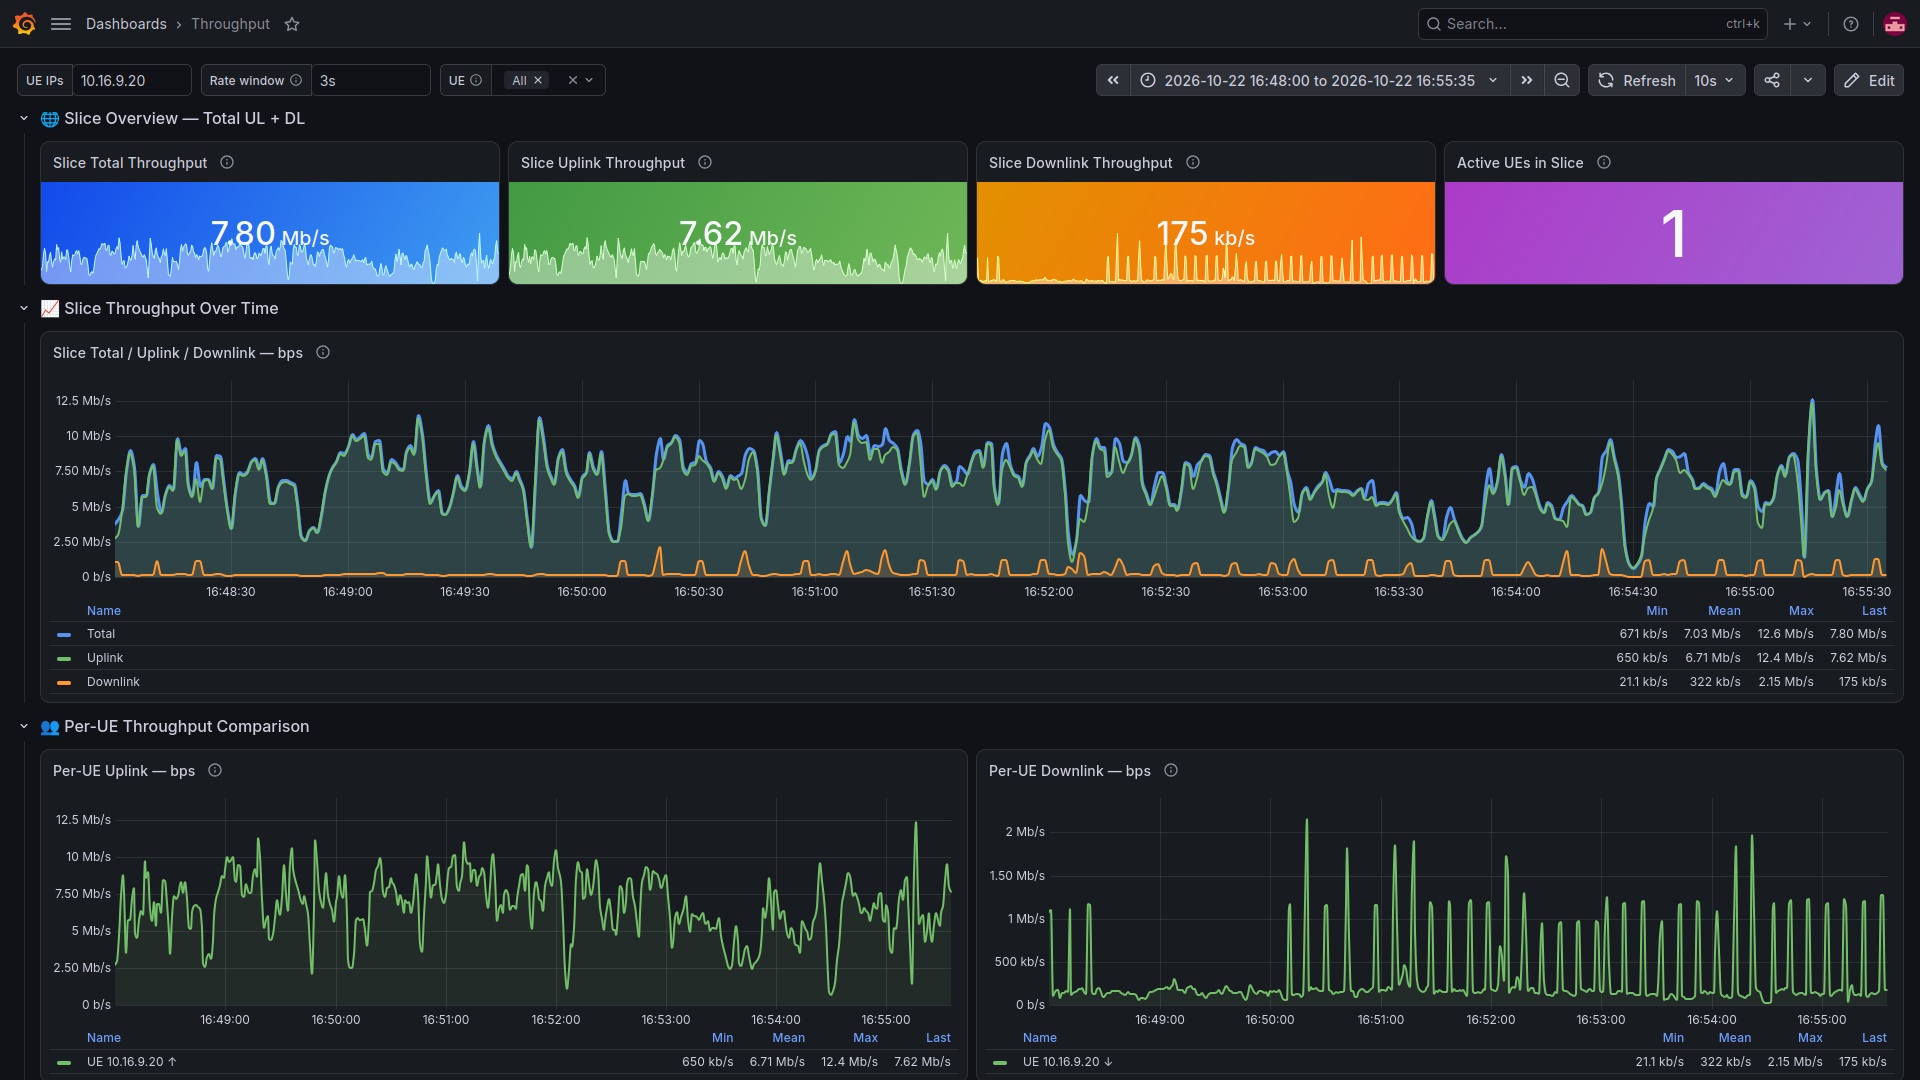
\includegraphics[width=1\linewidth]{granana_throughput_dashboard.png}
    \caption{Grafana slice throughput dashboard}
    \label{fig:impl:observability:dashboard:throughput}
\end{figure}

\begin{figure}[htpb]
    \centering
    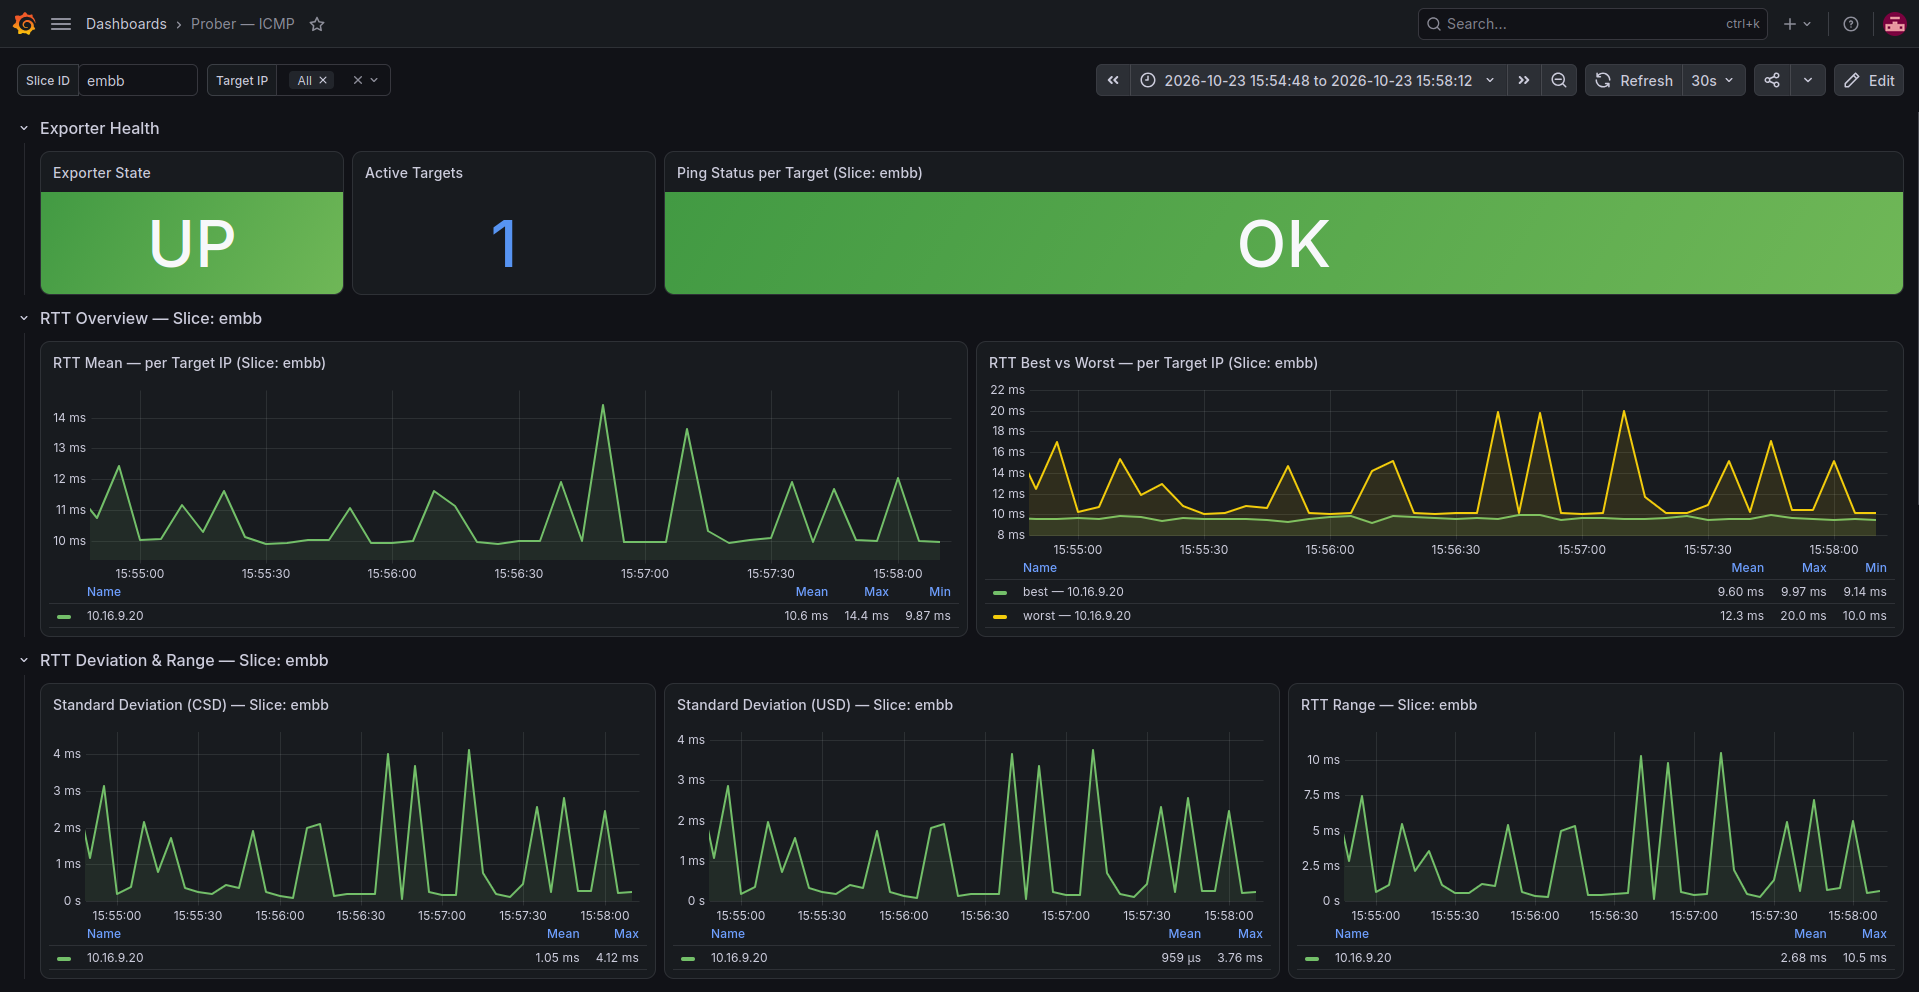
\includegraphics[width=1\linewidth]{grafana_prober_dashboard.png}
    \caption{Grafana active probing dashboard}
    \label{fig:impl:observability:dashboard:prober}
\end{figure}

In parallel, programmatic access through the \acs{NEF} AnalyticsExposure and CAMARA Connectivity Insights Subscriptions \acsp{API} outlined earlier is also provided. To achieve this, the \acs{NEF} queries the Prometheus \acs{HTTP} \acs{API} to derive near-real-time and historic analytics from the stored time series. For the probe measurements, e.g. \acs{RTT}, jitter \acs{RTT}, no equivalent programmatic exposure mechanism is currently available as, to the best of the authors' knowledge, neither the 5GC exposure interfaces nor the CAMARA initiative define a standardized \acs{API} for exposing metrics obtained exclusively from active probing procedures.

\section{Service Delivery}
\label{chap:impl:delivery}

\plan{
    \begin{enumerate}
        \item Start with a diagram where you present the various steps:
        \begin{itemize}
            \item app design
            \item network slice design
            \item onboarding
        \end{itemize}
        \item Establish
        \item Highlight
        \item Introduce
    \end{enumerate}
}


\section{Testbed Capabilities}
\label{chap:impl:capabilities}

Table~\ref{tab:impl:capabilities} summarizes the capabilities realized by the testbed, which essentially fulfill those proposed in Table~\ref{tab:proposal:capabilities} within the 5GAIner infrastructure. \acs{OSL} was chosen as the \acs{OSS}, through which all testbed services are ordered and managed via \acs{TMF} Open \acsp{API}, deploying containerized services on Kubernetes and delegating the orchestration of virtualized \acsp{NF} and applications to \acs{OSM}. The provisioning of network slices and \acsp{UE}, in turn, relies on the 5GAIner Slice Manager, which abstracts the lifecycle of network slices and \acs{UE} associations. Thus, the \acs{NSMF} and \acs{NSSMF} did not need to be implemented, being replaced by an \acs{OSL} Generic Controller that interacts with the Slice Manager.

The network exposure layer is realized by the \acs{NEF}Sim, and by the CAMARA \acsp{API}, implemented as a translation layer over the \acs{NEF} northbound interface. In particular, the \acs{NEF} AnalyticsExposure and the CAMARA Application Profiles and Connectivity Insights Subscriptions \acsp{API} were developed in this dissertation. Both components are published, discovered and invoked through Open\acs{CAPIF}, integrated on the provider and invoker sides by means of its \acs{SDK}.

As for network observability, since the 5GAIner \acs{5G} core does not expose monitoring \acsp{API}, passive monitoring relies on a Prometheus exporter that collects traffic volume and throughput from the mirrored traffic of the \acs{5G} System. Active monitoring is provided by an \acs{ICMP} prober, measuring the \acs{RTT}, \acs{RTT} jitter and packet loss of each probed \acs{UE}. The collected metrics are presented in Grafana dashboards, automatically provisioned per slice by \acs{OSL}.

Lastly, notification mechanisms are also provided. As in the proposal, the capabilities marked in the Use Case column are those exercised by the \acs{PoC}.

\begin{table}[htb!]
% Fraction of \linewidth taken by the Capability column; Requirements fits one functional and one non-functional requirement per line, Use Case is as wide as its header and Realization takes the remaining width
\newcommand{\capfrac}{0.2890}
\newlength{\reqwidth}
\newlength{\nclabelwidth}
\newlength{\ucwidth}
\newlength{\realwidth}
\newcommand{\realization}[1]{\multicolumn{2}{>{\RaggedRight\arraybackslash}p{\dimexpr\realwidth+\arrayrulewidth-2\tabcolsep\relax}|}{\leavevmode#1}}
% Category rows shaded with the same gray tone of the remaining tables, with \catpad of extra padding above and below the text
\newlength{\catpad}
\setlength{\catpad}{3pt}
\newcommand{\category}[1]{\rowcolor{gray!15}\multicolumn{5}{|l|}{\rule[\dimexpr-\arraystretch\dp\strutbox-\catpad\relax]{0pt}{\dimexpr\arraystretch\ht\strutbox+\arraystretch\dp\strutbox+2\catpad\relax}\textbf{\textit{#1}}}}
\centering
\small
\renewcommand{\arraystretch}{1.3}
% Remove booktabs vertical padding so that the vertical rules join the horizontal ones
\setlength{\aboverulesep}{0pt}
\setlength{\belowrulesep}{0pt}
\settowidth{\nclabelwidth}{CAMARA}%
\settowidth{\ucwidth}{\textbf{Case}}%
\addtolength{\ucwidth}{4pt}%
\settowidth{\reqwidth}{FR00, NFR0}%
\setlength{\realwidth}{\dimexpr\linewidth-\capfrac\linewidth-\reqwidth-2\tabcolsep-\ucwidth-2\tabcolsep-6\arrayrulewidth\relax}%
\begin{tabular}{|>{\RaggedRight\looseness=-1\arraybackslash}p{\capfrac\linewidth}|l|>{\RaggedRight\arraybackslash}p{\dimexpr\realwidth-\nclabelwidth-4\tabcolsep\relax}|>{\raggedright\arraybackslash}p{\reqwidth}|@{}>{\centering\arraybackslash}m{\ucwidth}@{}|}
\toprule
\textbf{Capability} & \multicolumn{2}{l|}{\textbf{Realization}} & \textbf{Require-}\newline\textbf{ments} & \multicolumn{1}{@{}>{\centering\arraybackslash}p{\ucwidth}@{}|}{\textbf{Use}\newline\textbf{Case}} \\
\midrule
\category{Resource Lifecycle Management and Service Delivery} \\
\midrule
Service design, ordering, provisioning and \acs{LCM} & \realization{OpenSlice \acs{OSS}, accessible via the user interface and \acs{TMF} Open \acsp{API}} & \ref{enum:fr:slice}, \ref{enum:nfr:packaging} & \checkmark \\
\hline
Provisioning of network slices with custom \acs{QoS} & \realization{5GAIner Slice Manager through an OpenSlice Generic Controller} & \ref{enum:fr:slice}, \ref{enum:nfr:uplink-bitrate} & \checkmark \\
\hline
Provisioning and association of \acs{UE} with provisioned slice & \realization{5GAIner Slice Manager through an OpenSlice Generic Controller} & \ref{enum:fr:slice}, \ref{enum:fr:stream} & \checkmark \\
\hline
Orchestration of containerized services & \realization{Deployment on Kubernetes via OpenSlice's CRIDGE component} & \ref{enum:nfr:packaging} & \checkmark \\
\hline
Orchestration of virtualized \acs{NF} and applications & \realization{Delegation to \acs{OSM} via \acs{ETSI} \acs{SOL}005} & \ref{enum:nfr:packaging} & \\
\midrule
\category{Network Exposure} \\
\midrule
Secure \acs{API} publication, discovery and invocation & \realization{\acs{CAPIF}, specifically Open\acs{CAPIF}} & \ref{enum:nfr:secure-exposure} & \checkmark \\
\hline
Declaration of application network quality thresholds & CAMARA & Application Profiles~\cite{CAMARAapis} & \ref{enum:fr:qos-profile}, \ref{enum:fr:monitoring-profile} & \checkmark \\
\hline
\multirow{2}{=}{Configuring~\acs{QoS} session for a device} & \acs{NEF} & AsSessionWithQoS~\cite{ETSI_TS_129_522_V18_11_0,ETSI_TS_129_122_V18_8_0} & \multirow{2}{=}{\ref{enum:fr:qos-request},~\ref{enum:fr:qos-change}, \ref{enum:nfr:qos-enforcement}} & \multirow{2}{*}{\checkmark} \\
\cline{2-3}
& CAMARA & Quality on Demand~\cite{CAMARAapis} & & \\
\hline
\multirow{2}{=}{Subscription~to network analytics} & \acs{NEF} & AnalyticsExposure~\cite{ETSI_TS_129_522_V18_11_0} & \multirow{2}{=}{\ref{enum:fr:monitoring}, \ref{enum:nfr:degradation-detection}} & \multirow{2}{*}{\checkmark} \\
\cline{2-3}
& CAMARA & Connectivity Insights\newline Subscriptions~\cite{CAMARAapis} & & \\
\hline
\multirow{2}{=}{Device location and geofencing notifications} & \acs{NEF} & MonitoringEvent~\cite{ETSI_TS_129_522_V18_11_0,ETSI_TS_129_122_V18_8_0} & \multirow{2}{=}{\ref{enum:fr:ue-tracking}} & \multirow{2}{*}{\checkmark} \\
\cline{2-3}
& CAMARA & Device Location~\cite{CAMARAapis} & & \\
\hline
\multirow{2}{=}{Device reachability and roaming notifications} & \acs{NEF} & MonitoringEvent~\cite{ETSI_TS_129_522_V18_11_0,ETSI_TS_129_122_V18_8_0} & \multirow{2}{=}{--} & \\
\cline{2-3}
& CAMARA & Roaming Status,\newline Reachability Status~\cite{CAMARAapis} & & \\
\hline
Traffic steering and other \acs{3GPP} procedures & \acs{NEF} & TrafficInfluence, PfdManagement, among others~\cite{ETSI_TS_129_522_V18_11_0,ETSI_TS_129_122_V18_8_0} & -- & \\
\midrule
\category{Network Observability} \\
\midrule
Passive traffic monitoring & \realization{Data path Prometheus exporter\newline(traffic volume and throughput)} & \ref{enum:fr:monitoring}, \ref{enum:nfr:degradation-detection} & \checkmark \\
\hline
Active monitoring & \realization{\acs{ICMP} prober\newline(\acs{RTT}, Packet Loss and \acs{RTT} jitter)} & \ref{enum:fr:monitoring}, \ref{enum:nfr:degradation-detection} & \checkmark \\
\hline
Monitoring Visualization & \realization{Grafana dashboards} & \ref{enum:nfr:logging} & \checkmark \\
\midrule
\category{Notification} \\
\midrule
Delivery of \acs{SMS} notifications to individual \acsp{UE} & \realization{Mock \acs{SMS} \acs{API}} & \ref{enum:fr:notify-pedestrians},~\ref{enum:fr:notify-periodic}, \ref{enum:nfr:notification-time} & \checkmark \\
\hline
Geographic message broadcast to vehicles & \realization{Geocast of \acsp{DENM} via a 5GAIner \acs{MQTT} broker with quadtree tiling} & \ref{enum:fr:notify-vehicles},~\ref{enum:fr:notify-periodic}, \ref{enum:nfr:notification-time} & \checkmark \\
\bottomrule
\end{tabular}
\caption{Summary of the realized testbed capabilities}
\label{tab:impl:capabilities}
\end{table}
\section{Multi-Vertical Use Case}
\label{chap:impl:use-case}

Section~\ref{chap:proposal:use-case} defined the functional and non-functional requirements for a vehicle collision detection and notification network application across the \acs{PPDR} and Automotive vertical sectors. Section~\ref{chap:proposal:capabilities} then identified the testbed capabilities required to support the development and validation of such a use case, and, most importantly, the exposure interfaces through which these capabilities can be made available to third parties. The implementation of the vertical application is presented next, explaining how the capabilities provided by the testbed, already detailed in Sections~\ref{chap:impl:resource_lifecycle} to~\ref{chap:impl:delivery}, are leveraged by the \acs{PoC} to fulfill the application requirements. In doing so, the \acs{PoC} serves as an end-to-end validation of the exposure interfaces and capabilities developed throughout the dissertation, while demonstrating their practical relevance in supporting the implementation and evaluation of future network applications.

Table~\ref{tab:testbed:capabilities} summarizes the testbed's capabilities, highlighting those exercised by this application. Network resources were reserved through the \acs{OSS} by provisioning a dedicated network slice with the uplink/downlink bitrate and latency guarantees needed to sustain continuous video streams from the roadside cameras to the inference server running the collision-detection model. Each camera, a \acs{5G} \acs{UE}, is identified by an \acs{IMSI} and attached to the previous network slice. During operation, network performance is continuously monitored through the testbed's passive monitoring system, presented in Grafana dashboards and also exposed through standardized interfaces, both orchestrated via the \acs{OSS}. The same \acs{OSS} provisions the network exposure components, such as the \acs{NEF} and CAMARA \acsp{API}, integrated with \acs{CAPIF}'s discovery, authentication and authorization workflows, which later support the application's interaction with the \acs{5G} network.

As a \acs{CAPIF} \acs{API} invoker, the application is able to discover and consume the \acsp{API} provided by \acs{NEF} and CAMARA that support the use case. For capabilities supported by both exposure models, the application can use either interface, allowing both alternatives to be exercised. The following sequence diagrams illustrate the interactions involved in the \acs{PoC} implementation for the two alternative \acs{API} exposure paths, prioritizing \acs{NEF}~in~Figure~\ref{chap:impl:use-case:flow:nef} and CAMARA~in~Figure~\ref{chap:impl:use-case:flow:camara}. The experimenter may opt out of the provisioning of the CAMARA component if only the \acs{NEF} is to be utilized, as previously described.

\begin{figure}[htbp]
    \centering
    
\includegraphics[width=1\linewidth]{figs/placeholder.png}
    \caption{\acs{PoC} sequence diagram via the \acs{NEF} exposure path}
    \label{chap:impl:use-case:flow:nef}
\end{figure}

The \acs{NEF} interactions are described first (Figure~\ref{chap:impl:use-case:flow:nef}). The network slice is provisioned beforehand through the \acs{OSS}, establishing the baseline connectivity for the application, i.e. the uplink streaming connection between the camera \acs{UE} and the inference server. However, to accommodate the stream's specific \acs{QoS} requirements and their variations over time (e.g. due to network contention), the \acs{PoC} interacts with the \acs{NEF} as part of the application workflow, using the AsSessionWithQoS \acs{API} to establish a \acs{QoS} session and dynamically adjust the connection's \acs{QoS} parameter as requirements change. The application can then continuously monitor the measured uplink throughput, consumed by the live video stream. This is achieved programmatically by creating an analytics subscription to periodically retrieve throughput measurements through the \acs{NEF} AnalyicsExposure \acs{API}, and the Prometheus integration mentioned in Section~\ref{chap:impl:observability}. When the observed metrics breach the \acs{KPI} thresholds for the defined \acs{QoS} level, it requests the enforcement of alternative \acs{QoS} profiles through the same AsSessionWithQoS \acs{API}, keeping the camera streams and detection model working as intended. This adaptation follows a reactive approach, as \acs{QoS} modifications are triggered only after \acs{KPI} violations have been detected. Nonetheless, in the future, \acs{QoS} predictions may be employed for a similar effect. In parallel to all of this, the application tracks pedestrian and vehicle \acs{UE} entering and leaving the monitored area through the \acs{NEF}'s MonitoringEvent \acs{API}.

When a collision is detected, the application triggers two emergency notifications. Pedestrians near the accident are notified via an \acs{SMS} alert delivered through a dedicated mock \acs{SMS} \acs{API}, using their \acs{MSISDN}. In parallel, nearby vehicles are notified through a \acs{DENM} delivered via an \acs{MQTT} broker, using a quadtree-based tiling scheme to relay the message to vehicles by geographic location. The \acs{MQTT} broker was provided separately by the existing 5GAIner infrastructure, whereas the mock \acs{SMS} \acs{API} was specifically developed for this application and included in the \acs{NEF} codebase. To clarify, this choice was made solely for practical reasons, as it avoids the need to deploy an additional component. No such \acs{API} is standardized in any of the \acs{NEF} specifications, something the author is fully aware of.

\begin{figure}[htbp]
    \centering
    
\includegraphics[width=1\linewidth]{figs/placeholder.png}
    \caption{\acs{PoC} sequence diagram via the CAMARA exposure path}
    \label{chap:impl:use-case:flow:camara}
\end{figure}

The CAMARA exposure path follows the same overall application workflow, but replaces the specific \acs{NEF} interfaces with the corresponding CAMARA \acsp{API} wherever equivalent capabilities are available. In particular, the \acs{PoC} uses the CAMARA \acs{QoD}, Connectivity Insights Subscriptions, and Device Location \acsp{API} to manage the session's \acs{QoS}, monitor network performance, and track devices in the geofenced area, respectively. Rather than interacting directly with the \acs{NEF}, the network application consumes these higher-level user-friendly CAMARA interfaces, and CAMARA (i.e., the CAMARA translation layer) internally translates the received requests into calls to the corresponding \acs{NEF} AsSessionWithQoS, AnalyticsExposure, and MonitoringEvent \acsp{API}, respectively.

Furthermore, the CAMARA component encapsulates additional logic that would otherwise fall under the responsibility of the network application developer. More specifically, when relying exclusively on the \acs{NEF}, the AnalyticsExposure and MonitoringEvent (\texttt{LOCATION\_REPORTING} event) \acsp{API} periodically retrieve the relevant metrics and location information, respectively, leaving the application to determine whether the measured \acsp{KPI} remain within the defined bounds and the reported locations, within the geofenced area.

With CAMARA, this responsibility shifts to the exposure layer. The application first declares its streaming requirements through the CAMARA Application Profiles \acs{API}, which registers an application profile describing the network conditions needed for the video stream to be processed reliably, namely the minimum upstream and downstream bitrate (i.e. \texttt{targetMinUpstreamRate}, \texttt{targetMinDownstreamRate}). The identifier of this profile is then included in the Connectivity Insights Subscriptions request, so the application no longer has to restate its thresholds whenever it subscribes (unlike AnalyticsExposure). CAMARA uses the referenced profile to evaluate the throughput measurements it receives from the \acs{NEF} and notifies the application only when the defined \acs{KPI} thresholds are breached. A similar event-driven approach applies to geofencing: the application subscribes to location events for the pedestrian and vehicle \acsp{UE} being monitored, and CAMARA notifies it only when a \acs{UE} enters or leaves the defined geofenced area. The application therefore reacts to explicit breach notifications instead of continuously inspecting the raw measurements or location coordinates, which keeps its logic simpler and focused on the use case itself. This is also particularly valuable given the complexity of the \acs{3GPP} data model and its procedures, which is especially evident in the AnalyticsExposure \acs{API}, given the high diversity of analytics event types and payloads.




the rest of the UEs (pedestrians, vehicle UEs are mocked and have their routes preplanned through the capabilities provided by NEFSim

don't forget to mention monitoring event caveat (have to reimplement part of the implementation from the other side)

Other things lack mentioning: 

- mediaMTX

- streaming process (with mediaMTX and ffmpeg)

- roboflow (ML detecting process)


we need like an architecture section to mention the actors and where they are 

The pedestrian and vehicle \acs{UE}s represent bystanders that do not contribute to network traffic and are therefore fully simulated using NEFSim. A population script\footnote{\url{https://github.com/Testbed-TNEI/VehicleDetectionPoC/blob/main/app/scripts/nef_db_init.sh}} is used to register these \acs{UE}s, alongside the actual camera \acs{UE} and the inference server's \acs{IP} address associated with the video stream.

are essentially bystanders that don't have any quote on network traffic, being completely simulated with NEFSim. Mention the 

- print of the dashboards with the stuff of the application

- notification driven 

\section{Chapter Summary}
\label{chap:impl:summary}

This chapter presented the realization of the proposed testbed on the 5GAIner infrastructure at \acs{ITAv}. Section~\ref{chap:impl:architecture} identified the concrete components behind each layer of the proposed architecture. \acs{OSL} serves as the single entry point for all testbed services, delegating the provisioning of \acs{5G} resources to \acs{ITAv}'s Slice Manager. Network capabilities are exposed by the \acs{NEF}Sim and CAMARA under Open\acs{CAPIF}, while network metrics are collected and visualized with Prometheus and Grafana.

Section~\ref{chap:impl:resource_lifecycle} addressed the lifecycle management of network slices and \acsp{UE}. Within the management hierarchy, \acs{OSL} fulfills the \acs{CSMF} role, while the \acs{NSMF} and \acs{NSSMF} functions are abstracted by the Slice Manager. To bridge both components, a Slicing Generic Controller was developed, translating the lifecycle events of the network slice and \acs{UE} resources into Slice Manager \acs{API} operations.

Regarding network exposure, Section~\ref{chap:impl:exposure} describes the implementation of the \acs{NEF}Sim and how it was extended in this dissertation to interact with the live network and the testbed's monitoring system. The \textit{AsSessionWithQoS} \acs{API} was adapted to the current Slice Manager \acs{API}, while the \textit{AnalyticsExposure} \acs{API} was developed from scratch to expose the collected network metrics in the absence of an \acs{NWDAF}. In addition, the CAMARA \textit{Application Profiles} and \textit{Connectivity Insights Subscriptions} \acsp{API} were implemented, as a simplified interface to obtain analytics capabilities and compare them to the application's requirements. All exposure interfaces were secured through the integration of Open\acs{CAPIF} on both the provider and invoker sides, using its \acs{SDK} to handle their publication, discovery and authorized invocation.

Section~\ref{chap:impl:observability} then detailed the monitoring system of the testbed. Since the 5GAIner \acs{5G} core provides no interfaces for exposing network metrics, passive monitoring relies on a Prometheus exporter that collects traffic metrics from mirrored traffic of the \acs{5G} data path. Active monitoring is provided by an \acs{ICMP} prober, selected among existing open source exporters, also compatible with Prometheus. The collected metrics are presented in Grafana dashboards provisioned per slice and are also made available programmatically through the \acs{NEF} and CAMARA analytics \acsp{API}.

Subsequently, Section~\ref{chap:impl:delivery} described how every testbed capability is offered as an orderable \acs{CFS} in \acs{OSL}, decomposed into one or more \acsp{RFS}. For the delivery of \acs{5G} resources, the Network Slice \acs{CFS} inherits the standardized attributes of the \acs{GSMA} \acs{GST}, while the \acs{UE} \acs{CFS} follows the minimal \acs{UE} blueprint in line with the specifications proposed in Section~\ref{chap:proposal:delivery}. These are fulfilled by the Slice Manager, whereas the remaining services follow a \acs{HaaS} approach. A bundle \acs{CFS} aggregates all services, provisioning a complete experiment through a single order according to the proposed dependency chain.

As summarized in Section~\ref{chap:impl:capabilities}, the realized testbed fulfills the capabilities proposed in Chapter~\ref{chap:proposal}, by mapping each capability to a concrete component. These mappings include (i)~the replacement of dedicated slice management functions by the Slice Manager and the Generic Controller, (ii)~the collection of traffic metrics on the data path in place of core monitoring interfaces and (iii)~the delivery of road user notifications through a mock \acs{SMS} and a \acs{V2X} \acs{MQTT} service.

Finally, Section~\ref{chap:impl:use-case} implemented the vehicle collision detection and notification application, utilizing the exposure capabilities of the testbed, namely the \acs{NEF} and CAMARA interfaces. The application was realized through both exposure paths, each of them sufficient to fulfill its requirements. This highlights the importance of the developed exposure capabilities, on which the application relies to observe the network conditions of its video streams and adapt their \acs{QoS} accordingly.


\chapter{Results and Validation}
\label{chap:results}

Having detailed the design and implementation of the testbed in the preceding chapters, it remains to demonstrate its ability to support the complete lifecycle of a network application experiment. In this chapter, the implemented testbed capabilities and network exposure interfaces are validated by deploying and evaluating the network application developed in Section~\ref{chap:impl:use-case} throughout the successive stages of an experiment, following the plan and guidelines outlined in Section~\ref{chap:proposal:validation}.

Before the network application can use the \acs{5G} network's capabilities, the testbed must deliver the requested network services, as configured by the experimenter. Section~\ref{chap:results:delivery} evaluates this delivery process by measuring the time required to deploy each requested service, including network slicing, network monitoring, network exposure, and the network application itself, until the experiment is ready for execution. This provides a reference for the setup cost that precedes any interaction with the \acs{5G} network.

Once the environment is fully deployed, the dissertation proceeds to the execution and validation of the network application, evaluating how the testbed supports its operation over the \acs{5G} network through a series of experiments. Section~\ref{chap:results:exposure} assesses the performance of the available network exposure interfaces, to request and/or enforce the specified network capabilities on the infrastructure. The latency of the supported operations is measured for both \acs{NEF} and CAMARA \acsp{API}, followed by a comparative analysis that quantifies the overhead introduced by the additional abstraction layer. Lastly, Section~\ref{chap:results:use-case} demonstrates how the testbed's capabilities can be leveraged collectively to validate the multi-vertical use case in an \acs{E2E} adaptive \acs{QoS} scenario. It further illustrates how the network exposure interfaces can be used to detect deteriorating network conditions and trigger \acs{QoS} adaptation to maintain and fulfill the application requirements.

\section{Service Delivery Performance}
\label{chap:results:delivery}

Experiment X

\subsection{Experimental Setup}
\label{chap:results:delivery:setup}

\subsection{Procedure}
\label{chap:results:delivery:procedure}

\subsection{Results and Discussion}
\label{chap:results:delivery:discussion}

\section{Network Exposure Benchmark and Comparison}
\label{chap:results:exposure}

Once the experiment is provisioned, the network application interacts with the \acs{5G} network through the exposure interfaces offered by the testbed, requesting and/or enforcing the network capabilities its use case depends on.

This experiment measures and compares the time required to complete the operations supported by both the \acs{NEF} and the CAMARA \acsp{API}, as experienced by the network application. The objective is to quantify the overhead introduced by the CAMARA abstraction layer, which internally consumes the \acs{NEF}, and to assess whether it represents an acceptable tradeoff for its simpler, developer-facing interfaces. The experiment also validates that both exposure models retrieve equivalent information from the network, allowing verticals to choose either interface according to the requirements of their application.

\subsection{Experimental Setup}
\label{chap:results:exposure:setup}

This experiment relies on the \acs{CAPIF},\acs{NEF}, and CAMARA services listed in Table~\ref{tab:impl:capabilities}, which are provisioned through OpenSlice alongside the network application. For this purpose, the application was deliberately configured to issue requests directly to the \acs{NEF} and the corresponding CAMARA \acsp{API}. As a \acs{CAPIF} \acs{API} invoker, the application discovers and consumes the \acsp{API} provided by the \acs{NEF} and CAMARA that support the use case, and, for capabilities supported by both exposure models, either interface can be used, allowing both alternatives to be exercised.

The testbed environment is the same as described in Section~\ref{chap:results:delivery:setup}, with OpenSlice and the Kubernetes cluster hosting the network exposure interfaces and the network application running on the same \acs{VM}. All other services, namely the throughput Prometheus exporter and the pcap pipeline, ran on a separate Ubuntu 22.04 \acs{VM} with 16 vCPUs, 32 GB \acs{RAM}, and 256 GB disk. Within the experimental setup illustrated in Figure~\ref{fig:results:experimentalsetup}, this experiment evaluates the network application and the exposure components deployed on the Kubernetes cluster, namely Open\acs{CAPIF}, the \acs{NEF}Sim and the CAMARA \acsp{API}, which interact with the Slice Manager and the Huawei \acs{5G} Core.

To ensure that every repetition follows an identical procedure, a Bash script was developed to automate the experiment, issuing the requests to each endpoint and recording the corresponding response times. Between consecutive runs, the script also deletes the resources created by the previous request (e.g. \acs{QoS} sessions and subscriptions), ensuring that each repetition starts from the same state and that no accumulated resources affect the measured times.

\subsection{Procedure}
\label{chap:results:exposure:procedure}

For each capability supported by both exposure models, the application issued the same operation through the \acs{NEF} and through the equivalent CAMARA \acs{API}, namely the creation of a \acs{QoS} session (\textit{AsSessionWithQoS} and \acs{QoD}), of an analytics subscription (\textit{AnalyticsExposure} and Connectivity Insights Subscriptions), and of a location subscription (\textit{MonitoringEvent} and Geofencing Subscriptions). The creation of application network requirements through the CAMARA Application Profiles \acs{API}, which has no \acs{NEF} counterpart, was also measured.

Each endpoint was invoked 30 consecutive times, alternating between the endpoints under test, with the repetitions issued in rapid succession so that the underlying \acs{HTTPS} connections to the corresponding Fast\acs{API} backends remained open and were reused. For each request, the enforcement time was recorded, together with the additional latency introduced by the CAMARA abstraction.

The response payloads obtained through both models were also compared and validated to confirm the same information is retrieved either way. Moreover, the analytics \acsp{API} were checked against generated synthetic traffic to confirm they reflected actual network activity.

\subsection{Results and Discussion}
\label{chap:results:exposure:discussion}

Table~\ref{tab:results:exposure:apis} reports the enforcement times for each operation, including the additional latency introduced by the CAMARA abstraction.


\begin{table}[htbp]
    \centering
    % 4 columns with 5 vertical bars and 8 instances of \tabcolsep, spanning the full \textwidth
    % The first column fits the longest API name in a single line
    % The remaining width is split equally among the other three columns
    \newlength{\expfirstcolw}
    \newlength{\expcolw}
    \settowidth{\expfirstcolw}{\textbf{\textit{AnalyticsExposure} / Connectivity Insights Subs.}}
    \setlength{\expcolw}{\dimexpr(\textwidth - 5\arrayrulewidth - 8\tabcolsep - \expfirstcolw)/3\relax}
    \begin{tabular}{|>{\RaggedRight\arraybackslash}m{\expfirstcolw}|>{\centering\arraybackslash}m{\expcolw}|>{\centering\arraybackslash}m{\expcolw}|>{\centering\arraybackslash}m{\expcolw}|}
        \hline
        \multicolumn{1}{|c|}{\diagbox[innerwidth=\expfirstcolw]{\acs{API}}{Interface}} &
        \textbf{\acs{NEF}} &
        \textbf{CAMARA} &
        \textbf{CAMARA}\newline\textbf{Overhead} \\
        \hline
        \textbf{\textit{AsSessionWithQoS} / \acs{QoD}}: Create \acs{QoS} Session & $28.392\,\pm$\newline$6.889$~ms & $45.014\,\pm$\newline$8.863$~ms & $18.280\,\pm$\newline$4.675$~ms \\
        \hline
        \textbf{Application Profiles}: Create Application Analytics Network Requirements & \textendash & $16.418\,\pm$\newline$4.044$~ms & \textendash \\
        \hline
        \textbf{\textit{AnalyticsExposure} / Connectivity Insights Subscriptions}: Create Subscription & $60.541\,\pm$\newline$13.815$~ms & $78.069\,\pm$\newline$19.532$~ms & $22.274\,\pm$\newline$7.905$~ms \\
        \hline
        \textbf{\textit{MonitoringEvent} / Geofencing Subscriptions}: Create Subscription & $29.678\,\pm$\newline$11.333$~ms & $42.031\,\pm$\newline$10.637$~ms & $17.486\,\pm$\newline$5.055$~ms \\
        \hline
    \end{tabular}
    \caption{Application Response Time Comparison for \acs{NEF} and CAMARA \acsp{API}}
    \label{tab:results:exposure:apis}
\end{table}

As expected, CAMARA requests consistently take longer than directly invoking the \acs{NEF}. Instead of interacting with the \acs{5G} network directly, CAMARA translates each request into a \acs{NEF} invocation and adapts the response to the CAMARA schema, so this \acs{NEF} segment accounts for most of the observed CAMARA path time, with the remainder corresponding to the abstraction's actual cost and the additional network call. Across the evaluated operations, this overhead ranged from approximately 17 to 22~ms. However, local testing indicated that this overhead should be even lower, at around 6 to 10~ms. This may result from a variety of factors. Unlike local testing, where containers run directly on localhost, the testbed utilizes a real Kubernetes deployment, in which requests between the CAMARA and \acs{NEF} services traverse the cluster network. In addition, the testbed runs on shared infrastructure, where concurrent workloads compete for the same computing and network resources, potentially increasing the observed response times.

Although not tested here, the same observation applies to notifications delivered back to the application. Events originating from CAMARA subscriptions introduce additional latency compared to equivalent \acs{NEF} subscriptions, since notifications must traverse both the \acs{NEF} and CAMARA services before reaching the application. This is aggravated by the fact that, according to their respective specifications, none of the \acs{QoS} Provisioning, Connectivity Insights Subscriptions and Device Location CAMARA \acsp{API} support subscriptions targeting more than a single device. Therefore, monitoring the pedestrian \acsp{UE} in the vicinity of the camera requires the application to create, track and delete a separate subscription for each device, each incurring the setup cost reported in Table~\ref{tab:results:exposure:apis}. Similarly, when a condition affects multiple devices, the application receives one notification per subscription rather than a single aggregated event. This deviates from what is supported by the current \acs{NEF} specification, which allows an external group identifier to be used as the target for a subscription.

The comparison of the response payloads confirmed that the same information is retrieved through both models, and the analytics \acsp{API} reflected the actual network activity. Overall, these results also demonstrate that the application could successfully interact with the network through both exposure interfaces.

Nonetheless, each exposure model has its own advantages and limitations. CAMARA's simple \acsp{API} make it the more immediate path for developers without telco expertise, when its scope matches the application's intent, at the cost of a few tens of milliseconds' overhead (Table~\ref{tab:results:exposure:apis}). This is a worthwhile tradeoff for most use cases given CAMARA's integration benefits, though it comes with less flexibility, as explained prior.

\subsection{Conclusions}
\label{chap:results:exposure:conclusion}

These results establish that the network application can request the aforementioned network capabilities through both exposure models, quantifying the response time of each operation offered by the \acs{NEF} and CAMARA \acsp{API}. The CAMARA abstraction layer consistently adds between 17 and 22~ms to each operation, while retrieving the same information as the \acs{NEF} through simpler, developer-friendly interfaces.

For a vertical developer, both exposure models may support the intended use case. The decision between them depends on whether CAMARA's simplicity suffices for the application goal and whether its overhead is an acceptable tradeoff. Since the testbed offers both interfaces, this decision is left to the application developer, driven by the vertical application's requirements rather than the testbed's capabilities, as it should be.

\section{Multi-Vertical Use Case in \acs{E2E} Adaptive QoS Scenario}
\label{chap:results:use-case}

The experiments presented in Section~\ref{chap:results:exposure} evaluated the performance and interaction model between the network application and the \acs{5G} network exposure interfaces provided by the testbed. However, these experiments focused on the performance of the exposure interfaces themselves, without assessing their impact on the underlying network or how the resulting network conditions affected the application components.


The requirements on slice based on specification X. However, in practice the streaming traffic resulted on an average of . Which was therefore set as the baseline for the streaming requiremenst and analytics window

\subsection{Experimental Setup}
\label{chap:results:use-case:setup}

\subsection{Procedure}
\label{chap:results:use-case:procedure}

\subsection{Results and Discussion}
\label{chap:results:use-case:discussion}

\subsection{Conclusions}
\label{chap:results:use-case:conclusion}

\section{Chapter Summary}
\label{chap:results:summary}


\chapter{Conclusions}
\label{chap:conclusions}

\input{chapters/chapter6/6.0-introduction}
\section{Contributions}
\label{chap:conclusions:contributions}

From the obtained results, it can be concluded that the objectives established for this dissertation have been achieved.

The implemented features extend the \acs{ITAv}'s \acs{NEF} beyond a purely simulated environment, allowing network applications to interact with the live \acs{5G} network. The adaptation of the \textit{AsSessionWithQoS} \acs{API} to the updated Slice Manager allows applications to request and change \acs{QoS} sessions on demand.

In turn, since the 5GAIner \acs{5G} core does not provide dedicated monitoring interfaces, an alternative monitoring mechanism was developed in this work, collecting network metrics directly from the \acs{5G} data path. This approach can be leveraged in any \acs{5G} deployment lacking such interfaces, without depending on the capabilities of the underlying core. Combined with the new \textit{AnalyticsExposure} \acs{API}, this mechanism collects and exposes the actual network conditions through a standardized interface, so that applications can verify whether the network meets their requirements.

On top of these \acs{NEF} capabilities, the Application Profiles and Connectivity Insights Subscriptions \acsp{API} extend \acs{ITAv}'s CAMARA implementation with these network insights, which were previously unavailable through this exposure model. Applications can declare their network quality thresholds and be notified when the network no longer meets them, without handling the complexity of the corresponding \acs{NEF} procedures.

Both exposure models were integrated with \acs{CAPIF}, so that network applications discover, authenticate and access them through a common set of procedures. Regarding service delivery, \acs{TMF} service specifications were developed for every orderable testbed capability, including network slices, \acsp{UE}, monitoring, \acs{CAPIF}, \acs{NEF} and CAMARA \acsp{API}, all delivered through the OpenSlice catalog and the \acs{TMF} Open \acsp{API}. This also constitutes an important outcome of the dissertation.

In particular, the network slice and \acs{UE} specifications accommodate the \acs{GSMA} \acs{GST}, while retaining the characteristics specific to the \acs{ITAv}'s Slice Manager. Verticals, and further experimenters at \acs{ITAv}, can thus rely on these data models to define their network slices and configure the capabilities on the 5GAIner infrastructure. The same applies to the developed network application.

Last, but certainly not least, the work presented in this dissertation culminated in the publication, as the main author, of a conference paper at the \acs{IEEE} Future Networks World Forum 2026, entitled 'An Open \acs{5G} Testbed for Vertical Application Development and Experimentation'. The corresponding reference is highlighted below.

\begin{quote}
    \textbf{Figueiredo, Miguel} \& Direito, Rafael \& Gomes, Diogo \& Aguiar, Rui. (2026). \newline \textit{An Open 5G Testbed for Vertical Application Development and Experimentation}.
\end{quote}

\section{Future Work}
\label{chap:conclusions:future}

The testbed implemented in this dissertation establishes a solid foundation for the development, operation and validation of network applications and its interaction with the \acs{5G} network, through the exposure of network interfaces based on the \acs{TMF} \acs{ODA}, \acs{NEF}, CAMARA and \acs{CAPIF} standards. Nevertheless, the testbed could be further improved to expand the set of capabilities available to vertical experimenters.

Future work would extend these capabilities toward closed-loop automation. The testbed's observability layer follows a purely reactive model, notifying applications of changes in network conditions only after they occur. Integrating an \acs{NWDAF} would address this by using the metrics already collected and exposed via the \acs{NEF} as input for predictive analytics. The AnalyticsExposure and Connectivity Insights Subscriptions interfaces could then be extended with this predictive data, allowing applications to act proactively before network conditions affect or compromise their services.

The validation procedures, defined in Section~\ref{chap:proposal:validation}, would also benefit from greater automation. Testing could therefore be automated by the testbed and offered through the \acs{OSS} as part of the experiment. To this end, the testbed could automatically collect network monitoring metrics, application and orchestration logs, and exposure \acs{API} responses from the deployed services, comparing them against the expected values, such as the attributes of the ordered \acs{NEST} or the application \acsp{KPI}. This could be implemented through a \acs{CI} platform properly integrated with the \acs{OSS}, through which verticals would configure and execute the test cases for their experiments. It would also open the possibility for multi-stage testing pipelines, in which each service can be validated independently in isolation before the next one is deployed and validated alongside it.

For consistency with the rest of the testbed, such a pipeline would also rely on \acs{TMF} Open \acsp{API} and natively integrate with OpenSlice, the testbed's \acs{OSS}. Test cases could be declared and configured through the \acs{TMF} 653 \acs{API} (Service Test Management), alongside the services ordered through the \acs{TMF} 641 \acs{API} (Service Ordering)~\cite{openAPIsTMF}. The resulting verdicts would be aggregated into reports associated with the corresponding service instances and made available to vertical experimenters through OpenSlice.



%%%%%%%%%%%%%%%%%%%%%%%%%%%%%%%%%%%%%%%%%%%%%%%%%%%%%%%
% Print all used references
%%%%%%%%%%%%%%%%%%%%%%%%%%%%%%%%%%%%%%%%%%%%%%%%%%%%%%%

\begingroup
\renewcommand{\bibfont}{\footnotesize}
% Redefine References name to Portuguese
% Change if you are using english
\setsecnumdepth{none}
\maxsecnumdepth{none}

\defbibheading{bibliography}[Referências]{
\chapter{References}
}
\vspace{2em}
\SingleSpacing
\setlength\bibitemsep{8pt}
\printbibliography[heading=bibliography]

\setsecnumdepth{subsubsection}
\maxsecnumdepth{subsubsection}
\endgroup


%%%%%%%%%%%%%%%%%%%%%%%%%%%%%%%%%%%%%%%%%%%%%%%%%%%%%%%
% Load appendix
%%%%%%%%%%%%%%%%%%%%%%%%%%%%%%%%%%%%%%%%%%%%%%%%%%%%%%%

\mainmatterWithoutReset
\appendix
\pagestyle{plain}
\chapter{Additional Information}
\label{chap:appendix-more}

\section{NEF Implementations} \label{appendix:NEF}

\begin{longtable}{p{6cm} c c c}
\caption{Northbound \acs{API} Coverage across open source \acs{NEF} Implementations}
\label{tab:nef:comparision:long}\\
\toprule
\textbf{Northbound \acs{API}} & \textbf{Free5GC} & \textbf{NEFSim} \\
\midrule
\endfirsthead

\multicolumn{3}{c}%
{\tablename\ \thetable\ -- \textit{Continued from previous page}} \\
\toprule
\textbf{Northbound \acs{API}} & \textbf{Free5GC} & \textbf{NEFSim} \\
\midrule
\endhead

\midrule
\multicolumn{3}{r}{\textit{Continued on next page}} \\
\endfoot

\bottomrule
\endlastfoot

\rowcolor{gray!15}
ResourceManagementOfBdt      & $\times$             & $\times$ \\
\rowcolor{white}
PfdManagement                & $\checkmark$         & $\checkmark$ \\
\rowcolor{gray!15}
MonitoringEvent              & $\times$             & $\checkmark$ \\
\rowcolor{white}
DeviceTriggering             & $\times$             & $\times$ \\
\rowcolor{gray!15}
CpProvisioning               & $\times$             & $\times$ \\
\rowcolor{white}
ChargeableParty              & $\times$             & $\times$ \\
\rowcolor{gray!15}
AsSessionWithQoS             & $\times$             & $\checkmark$ \\
\rowcolor{white}
MsisdnLessMoSms              & $\times$             & $\times$ \\
\rowcolor{gray!15}
NpConfiguration              & $\times$             & $\times$ \\
\rowcolor{white}
NIDD                         & $\times$             & $\times$ \\
\rowcolor{gray!15}
RacsParameterProvisioning    & $\times$             & $\times$ \\
\rowcolor{white}
ECRControl                   & $\times$             & $\times$ \\
\rowcolor{gray!15}
TrafficInfluence             & $\checkmark$         & $\checkmark$ \\
\rowcolor{white}
NiddConfigurationTrigger     & $\times$             & $\times$ \\
\rowcolor{gray!15}
AnalyticsExposure            & $\times$             & $\times$ \\
\rowcolor{white}
5GLANParameterProvision      & $\times$             & $\times$ \\
\rowcolor{gray!15}
ApplyingBdtPolicy            & $\times$             & $\times$ \\
\rowcolor{white}
IPTVConfiguration            & $\times$             & $\times$ \\
\rowcolor{gray!15}
LpiParameterProvision        & $\times$             & $\times$ \\
\rowcolor{white}
ServiceParameter             & $\times$             & $\times$ \\
\rowcolor{gray!15}
ACSParameterProvision        & $\times$             & $\times$ \\
\rowcolor{white}
MoLcsNotify                  & $\times$             & $\times$ \\
\rowcolor{gray!15}
AKMA                         & $\times$             & $\times$ \\
\rowcolor{white}
TimeSyncExposure             & $\times$             & $\times$ \\
\rowcolor{gray!15}
EcsAddressProvision          & $\times$             & $\times$ \\
\rowcolor{white}
AMPolicyAuthorization        & $\times$             & $\times$ \\
\rowcolor{gray!15}
AMInfluence                  & $\times$             & $\times$ \\
\rowcolor{white}
MBSTMGI                      & $\times$             & $\times$ \\
\rowcolor{gray!15}
MBSSession                   & $\times$             & $\times$ \\
\rowcolor{white}
EASDeployment                & $\times$             & $\times$ \\
\rowcolor{gray!15}
ASTI                         & $\times$             & $\times$ \\
\rowcolor{white}
DataReporting                & $\times$             & $\times$ \\
\rowcolor{gray!15}
DataReportingProvisioning    & $\times$             & $\times$ \\
\rowcolor{white}
UEId                         & $\times$             & $\times$ \\
\rowcolor{gray!15}
MBSUserService               & $\times$             & $\times$ \\
\rowcolor{white}
MBSUserDataIngestSession     & $\times$             & $\times$ \\
\rowcolor{gray!15}
MSEventExposure              & $\times$             & $\times$ \\
\rowcolor{white}
MBSGroupMsgDelivery          & $\times$             & $\times$ \\
\rowcolor{gray!15}
DNAIMapping                  & $\times$             & $\times$ \\
\rowcolor{white}
PDTQPolicyNegotiation        & $\times$             & $\times$ \\
\rowcolor{gray!15}
MemberUESelectionAssistance  & $\times$             & $\times$ \\
\rowcolor{white}
GroupParametersProvisioning  & $\times$             & $\times$ \\
\rowcolor{gray!15}
SliceParamProvision          & $\times$             & $\times$ \\
\rowcolor{white}
UEAddress                    & $\times$             & $\times$ \\
\rowcolor{gray!15}
ECSAddress                   & $\times$             & $\times$ \\
\rowcolor{white}
RSLPPIParametersProvisioning & $\times$             & $\times$ \\
\end{longtable}

\clearpage
\section{Slice Manager \acs{API} Payloads}
\label{appendix:slicemanager:payloads}

\begin{listing}[H]
\begin{minted}{json}
{
  "slice_id": "embb-slice",
  "coverage_area": ["it"],
  "sst": 1,
  "sd": "020202",
  "dnn": "embb",
  "priority_label": 1,
  "ue_mobility_level": "nomadic",
  "reliability": 99.9,
  "uplink_max_packet_size_bytes": 1500,
  "downlink_max_packet_size_bytes": 1500,
  "scheduling_type": "BASIC_SCH",
  "downlink_min_resource_block_ratio": 10,
  "downlink_max_resource_block_ratio": 50,
  "uplink_min_resource_block_ratio": 10,
  "uplink_max_resource_block_ratio": 50,
  "downlink_latency_ms": 15,
  "uplink_latency_ms": 15,
  "delay_tolerance": "NOT_SUPPORTED",
  "downlink_deterministic_communication": "NOT_SUPPORTED",
  "downlink_deterministic_periodicity": null,
  "uplink_deterministic_communication": "NOT_SUPPORTED",
  "uplink_deterministic_periodicity": null,
  "downlink_guaranteed_bitrate_per_ue_kbps": 1000,
  "uplink_guaranteed_bitrate_per_ue_kbps": 1000,
  "downlink_maximum_bitrate_per_ue_kbps": 20000,
  "uplink_maximum_bitrate_per_ue_kbps": 20000,
  "downlink_guaranteed_bitrate_per_slice_kbps": 10000,
  "uplink_guaranteed_bitrate_per_slice_kbps": 10000,
  "downlink_maximum_bitrate_per_slice_kbps": 200000,
  "uplink_maximum_bitrate_per_slice_kbps": 200000,
  "terminal_density": 100,
  "max_number_of_pdu_sessions": 20,
  "max_number_of_ues": 10,
  "n6_protection": [
    {
      "type": "firewall",
      "name": "allow-video-ingest",
      "priority": 1,
      "server_ip": "10.16.9.10",
      "mask_len": 32,
      "start_port": 443,
      "end_port": 443,
      "uplink_guaranteed_bitrate_kbps": 10000,
      "downlink_guaranteed_bitrate_kbps": 50000,
      "uplink_maximum_bitrate_kbps": 20000,
      "downlink_maximum_bitrate_kbps": 100000,
      "protocol": "tcp",
      "pass_block": "pass"
    }
  ]
}
\end{minted}
\caption{Network Slice Payload, Slice Manager \acs{API}}
\label{code:slicemanager:payloads:netslice}
\end{listing}
\clearpage

\begin{listing}[H]
\begin{minted}{json}
{
  "slice_id": "embb-slice",
  "snssai": "1-020202",
  "dnn": "embb",
  "static_ipv4_address": "10.16.9.5",
  "access_mobility_data": true,
  "snssai_advertisement_allowed": true,
  "uplink_aggregate_maximum_bitrate_kbps": 1000,
  "downlink_aggregate_maximum_bitrate_kbps": 3000
}
\end{minted}
\caption{User Equipment Slice Association Payload, Slice Manager \acs{API}, with the \acs{IMSI} provided as \texttt{ue\_id} path parameter}
\label{code:slicemanager:payloads:ue}
\end{listing}

\clearpage
\section{\acs{PoC} Operation Sequence Diagrams}
\label{appendix:poc:operation}

\begin{figure}[htbp]
    \centering
    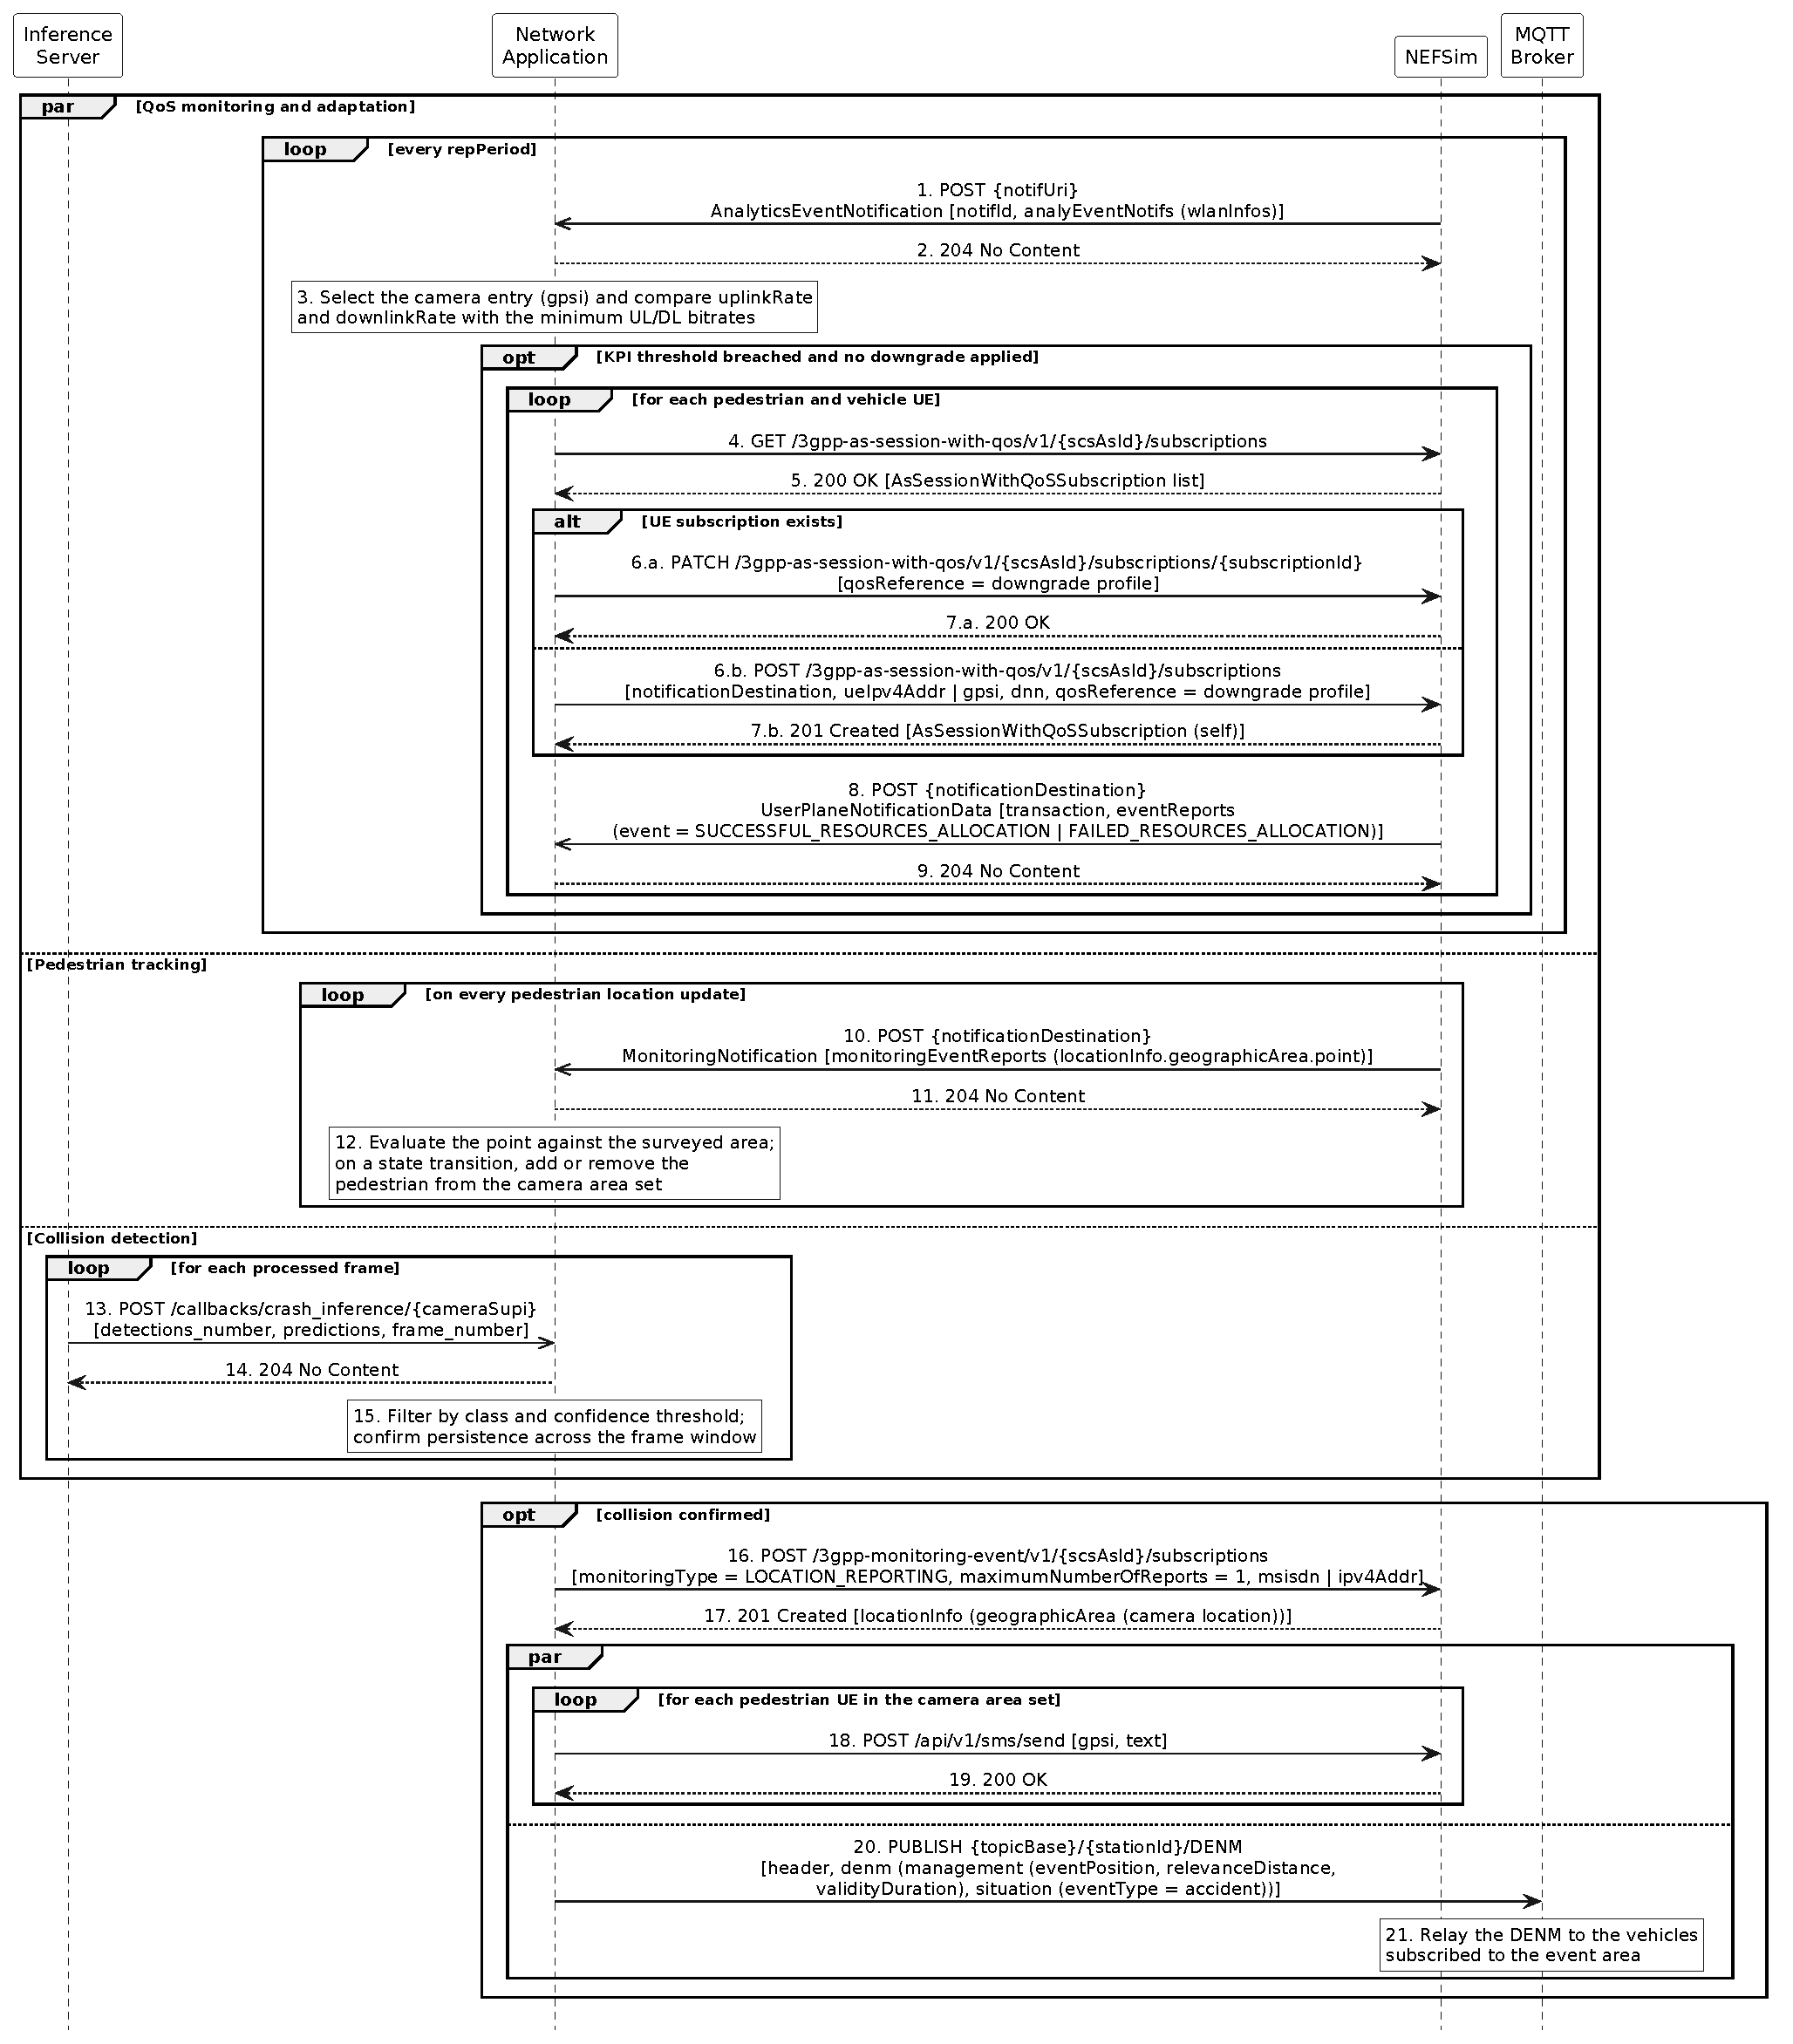
\includegraphics[width=1\linewidth]{figs/plantuml/poc-nef-operation-sequence.pdf}
    \caption{\acs{PoC} operation sequence diagram via the \acs{NEF} exposure path}
    \label{chap:impl:use-case:flow:nef:operation}
\end{figure}

\begin{figure}[htbp]
    \centering
    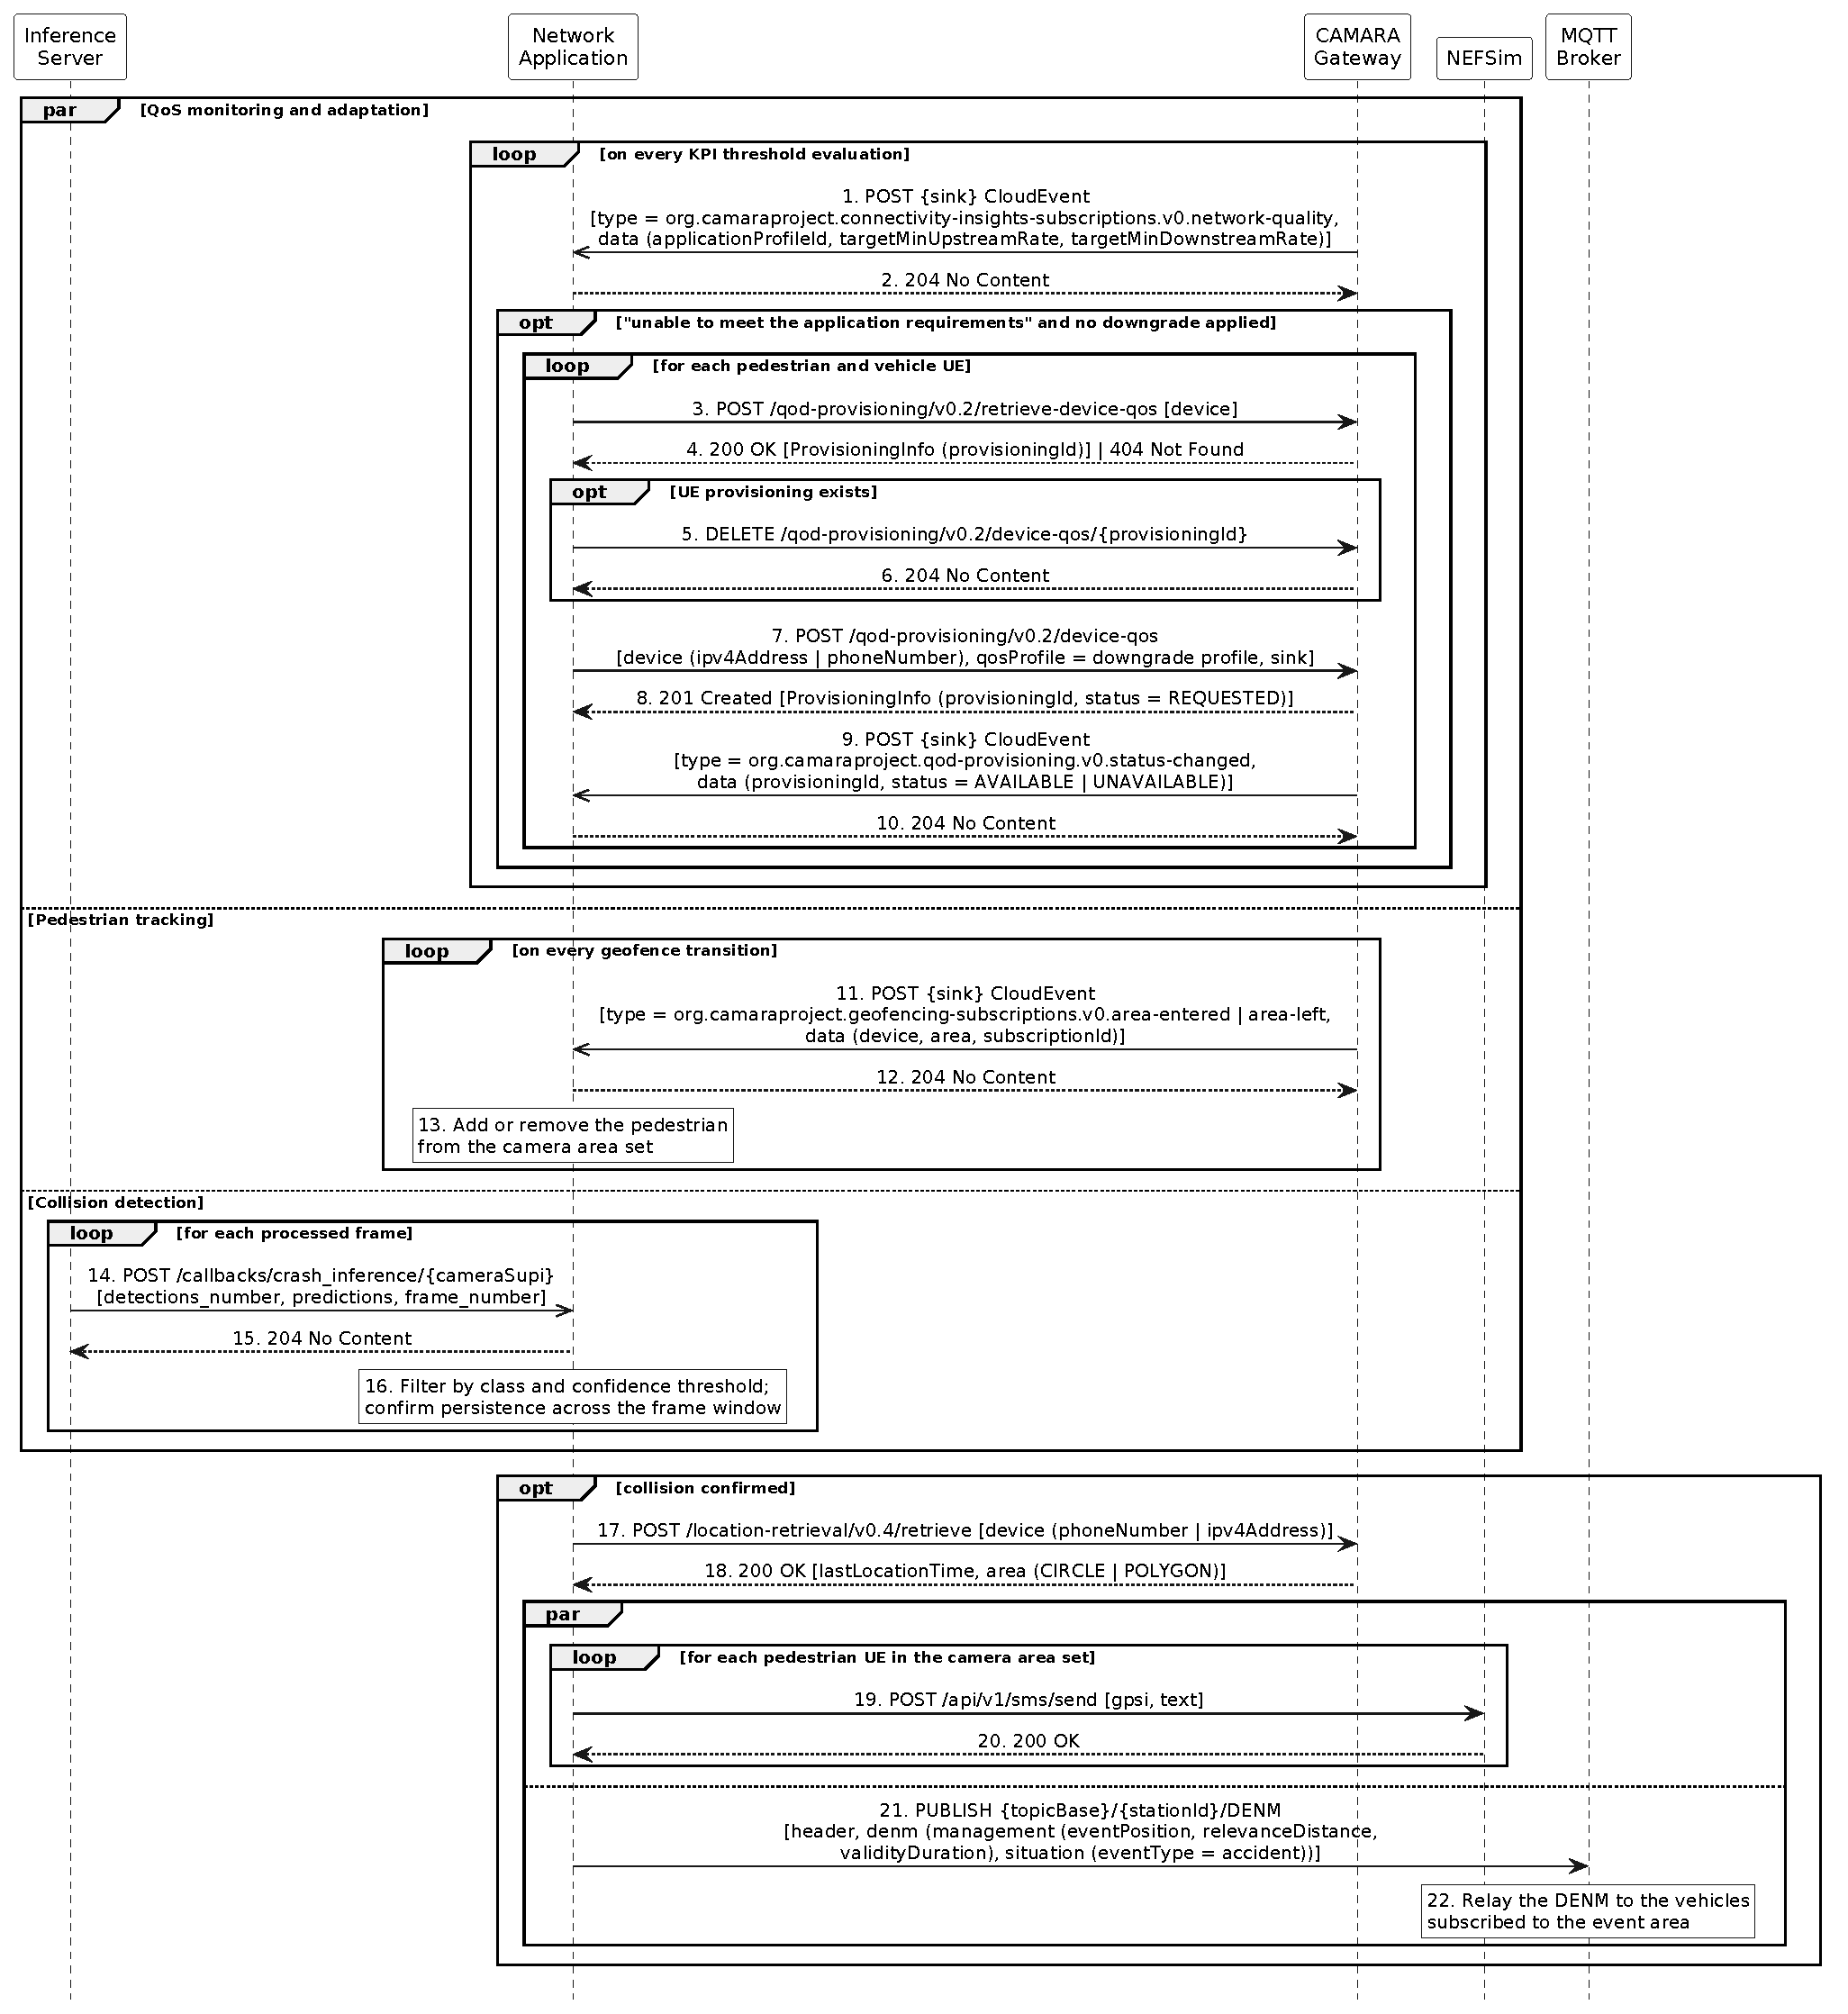
\includegraphics[width=1\linewidth]{figs/plantuml/poc-camara-operation-sequence.pdf}
    \caption{\acs{PoC} operation sequence diagram via the CAMARA exposure path}
    \label{chap:impl:use-case:flow:camara:operation}
\end{figure}

\end{document}